% -*- Mode:TeX -*-
\documentclass[12pt,twoside]{mitthesis}
\usepackage{lgrind}
%% These have been added at the request of the MIT Libraries, because
%% some PDF conversions mess up the ligatures.  -LB, 1/22/2014
\usepackage{cmap}
\usepackage[T1]{fontenc}
\pagestyle{plain}
%\usepackage{graphics} %% uncomment when i actually fix the errors
\usepackage{graphicx}
\usepackage{caption}
\usepackage{subcaption}
\usepackage{cancel}
\usepackage{adjustbox}
\usepackage{amsmath}
\usepackage{cite}
\usepackage{notoccite}
\usepackage{xspace}
\usepackage{tabularx}
\usepackage{dcolumn}

\usepackage[left]{lineno}

%% how to get the stupid references in right order

% \bibliographystyle{unsrt}
%% also need to do something about the ordering if there are citations in figures

%%%%%%%%%%%%%%%%%%%%%%%%%%%%%%%%%%%
\newcommand{\chapquote}[3]{\begin{quotation}\textit{#1} \end{quotation}\begin{flushright} - #2, \textit{#3}\end{flushright} }

%%%%% Units, Variables, misc.
\newcommand{\pt}{\ensuremath{p_{\mathrm{T}}}\xspace}
\newcommand{\et}{\ensuremath{E_{\mathrm{T}}}\xspace}
\newcommand{\met}{\ensuremath{E_{\mathrm{T}}^{miss}}\xspace}
\newcommand{\vmet}{\ensuremath{\vec{E}_{\mathrm{T}}^{miss}}\xspace}
\newcommand{\mt}{\ensuremath{m_{\mathrm{T}}}\xspace}
\newcommand{\invpb}{\ensuremath{\,\mathrm{pb}^{-1}}\xspace}
\newcommand{\pb}{\ensuremath{\,\mathrm{pb}}\xspace}
\newcommand{\mll}{\ensuremath{\mathrm{M}_{ll}}\xspace}
\newcommand{\s}{\ensuremath{\sqrt{s}}\xspace}
\newcommand{\nsig}{\ensuremath{N_{sig}}\xspace}
\newcommand{\sbr}{\ensuremath{\sigma \times Br}\xspace}
\newcommand{\TeV}{\ensuremath{\,\text{Te\hspace{-.08em}V}}\xspace}
\newcommand{\GeV}{\ensuremath{\,\text{Ge\hspace{-.08em}V}}\xspace}
\newcommand{\sg}{\ensuremath{\sqrt{s}=5.02\TeV}\xspace}
\newcommand{\sh}{\ensuremath{\sqrt{s}=13\TeV}\xspace}

\newcommand{\ns}{\ensuremath{\,\text{ns}}\xspace}

\newcommand{\rwpm}{\ensuremath{R_{\Wp/\Wm}}\xspace}
\newcommand{\rwpz}{\ensuremath{R_{\Wp/\Z}}\xspace}
\newcommand{\rwmz}{\ensuremath{R_{\Wm/\Z}}\xspace}
\newcommand{\rwz}{\ensuremath{R_{\W/\Z}}\xspace}

\newcommand{\lumig}{\ensuremath{291.1\pm 10 \invpb}\xspace}
\newcommand{\lumih}{\ensuremath{199.3\pm 4 \invpb}\xspace}

\newcommand{\GEANTfour} {{\textsc{Geant4}}\xspace}
\newcommand{\MINLO} {\textsc{MINLO}\xspace}
\newcommand{\MADGRAPH} {\textsc{MadGraph}\xspace}
\newcommand{\aMCATNLO} {a\textsc{mc@nlo}\xspace}
\newcommand{\MCATNLO} {\textsc{mc@nlo}\xspace}
\newcommand{\MGvATNLO}{\MADGRAPH{}5\_a\MCATNLO}
\newcommand{\PHOTOS} {\textsc{photos}\xspace}
\newcommand{\POWHEG} {{\textsc{powheg}}\xspace}
\newcommand{\PYTHIA} {{\textsc{pythia}}\xspace}

\newcommand{\masswindow}{\ensuremath{60\GeV\leq \mathrm{M}_{ll}\leq 120\GeV}\xspace}
\newcommand\barparen[1]{\overset{(-)}{#1}}

\newcommand{\uprp}{\ensuremath{u_{\perp}}\xspace}
\newcommand{\upar}{\ensuremath{u_{||}}\xspace}
\newcommand{\muf}{\ensuremath{\mu_{F}}\xspace}
\newcommand{\mur}{\ensuremath{\mu_{R}}\xspace}
%%%%% quark pairs, proton stuff, etc

\newcommand{\pp}{\ensuremath{pp}\xspace}
\newcommand{\ppbar}{\ensuremath{p\bar{p}}\xspace}
\newcommand{\qqbar}{\ensuremath{q\bar{q}}\xspace}
\newcommand{\udbar}{\ensuremath{u\bar{d}}\xspace}
\newcommand{\dubar}{\ensuremath{d\bar{u}}\xspace}
\newcommand{\ttbar}{\ensuremath{t\bar{t}}\xspace}


%% Bosons: 
\newcommand{\Z}{\ensuremath{Z}\xspace}
\newcommand{\W}{\ensuremath{W}\xspace}
\newcommand{\Zzero}{\ensuremath{\Z^0}\xspace}
\newcommand{\Wpm}{\ensuremath{\W^{\pm}}\xspace}
\newcommand{\Wp}{\ensuremath{\W^+}\xspace}
\newcommand{\Wm}{\ensuremath{\W^-}\xspace}

%% Z decays
\newcommand{\zmm}{\ensuremath{\Z\to\mu\mu}\xspace}
\newcommand{\zee}{\ensuremath{\Z\to e e}\xspace}
\newcommand{\zll}{\ensuremath{\Z\to \ell \ell}\xspace}

\newcommand{\ztt}{\ensuremath{Z\to\tau\tau}\xspace}

%% W decays
\newcommand{\wlnu}{\ensuremath{\W\to \ell \nu}\xspace}
\newcommand{\wenu}{\ensuremath{\W\to e \nu}\xspace}
\newcommand{\wmunu}{\ensuremath{\W\to \mu \nu}\xspace}
\newcommand{\wtau}{\ensuremath{\W\to \tau \nu}\xspace}

\newcommand{\wlp}{\ensuremath{\W^+\to \ell^+ \nu}\xspace}
\newcommand{\wep}{\ensuremath{\W^+\to e^+ \nu}\xspace}
\newcommand{\wmp}{\ensuremath{\W^+\to \mu^+ \nu}\xspace}

\newcommand{\wlm}{\ensuremath{\W^-\to \ell^- \nu}\xspace}
\newcommand{\wem}{\ensuremath{\W^-\to e^- \nu}\xspace}
\newcommand{\wmm}{\ensuremath{\W^-\to \mu^- \nu}\xspace}


\linenumbers

%% This bit allows you to either specify only the files which you wish to
%% process, or `all' to process all files which you \include.

%%\typein [\files]{Enter file names to process, (chap1,chap2 ...), or `all' to
%%process all files:}
%%\def\all{all}
%%\ifx\files\all \typeout{Including all files.} \else \typeout{Including only \files.} \includeonly{\files} \fi

\begin{document}

% -*-latex-*-
% 
% For questions, comments, concerns or complaints:
% thesis@mit.edu
% 
%
% $Log: cover.tex,v $
% Revision 1.8  2008/05/13 15:02:15  jdreed
% Degree month is June, not May.  Added note about prevdegrees.
% Arthur Smith's title updated
%
% Revision 1.7  2001/02/08 18:53:16  boojum
% changed some \newpages to \cleardoublepages
%
% Revision 1.6  1999/10/21 14:49:31  boojum
% changed comment referring to documentstyle
%
% Revision 1.5  1999/10/21 14:39:04  boojum
% *** empty log message ***
%
% Revision 1.4  1997/04/18  17:54:10  othomas
% added page numbers on abstract and cover, and made 1 abstract
% page the default rather than 2.  (anne hunter tells me this
% is the new institute standard.)
%
% Revision 1.4  1997/04/18  17:54:10  othomas
% added page numbers on abstract and cover, and made 1 abstract
% page the default rather than 2.  (anne hunter tells me this
% is the new institute standard.)
%
% Revision 1.3  93/05/17  17:06:29  starflt
% Added acknowledgements section (suggested by tompalka)
% 
% Revision 1.2  92/04/22  13:13:13  epeisach
% Fixes for 1991 course 6 requirements
% Phrase "and to grant others the right to do so" has been added to 
% permission clause
% Second copy of abstract is not counted as separate pages so numbering works
% out
% 
% Revision 1.1  92/04/22  13:08:20  epeisach

% NOTE:
% These templates make an effort to conform to the MIT Thesis specifications,
% however the specifications can change.  We recommend that you verify the
% layout of your title page with your thesis advisor and/or the MIT 
% Libraries before printing your final copy.
\title{Measurement of \W and \Z boson \\ production cross sections in \pp collisions \\ at \serag and \serah}

\author{Stephanie Akemi Brandt}
% If you wish to list your previous degrees on the cover page, use the 
% previous degrees command:
%       \prevdegrees{A.A., Harvard University (1985)}
% You can use the \\ command to list multiple previous degrees
%       \prevdegrees{B.S., University of California (1978) \\
%                    S.M., Massachusetts Institute of Technology (1981)}
\department{Department of Physics}

% If the thesis is for two degrees simultaneously, list them both
% separated by \and like this:
% \degree{Doctor of Philosophy \and Master of Science}
\degree{Doctor of Philosophy}

% As of the 2007-08 academic year, valid degree months are September, 
% February, or June.  The default is June.
\degreemonth{January}
\degreeyear{2020}
\thesisdate{December 31, 2019}

%% By default, the thesis will be copyrighted to MIT.  If you need to copyright
%% the thesis to yourself, just specify the `vi' documentclass option.  If for
%% some reason you want to exactly specify the copyright notice text, you can
%% use the \copyrightnoticetext command.  
%\copyrightnoticetext{\copyright IBM, 1990.  Do not open till Xmas.}

% If there is more than one supervisor, use the \supervisor command
% once for each.
\supervisor{Philip  Harris}{Assistant Professor of Physics}

% This is the department committee chairman, not the thesis committee
% chairman.  You should replace this with your Department's Committee
% Chairman.
\chairman{Nergis Mavalvala}{Associate Department Head of Physics}

% Make the titlepage based on the above information.  If you need
% something special and can't use the standard form, you can specify
% the exact text of the titlepage yourself.  Put it in a titlepage
% environment and leave blank lines where you want vertical space.
% The spaces will be adjusted to fill the entire page.  The dotted
% lines for the signatures are made with the \signature command.
\maketitle

% The abstractpage environment sets up everything on the page except
% the text itself.  The title and other header material are put at the
% top of the page, and the supervisors are listed at the bottom.  A
% new page is begun both before and after.  Of course, an abstract may
% be more than one page itself.  If you need more control over the
% format of the page, you can use the abstract environment, which puts
% the word "Abstract" at the beginning and single spaces its text.

%% You can either \input (*not* \include) your abstract file, or you can put
%% the text of the abstract directly between the \begin{abstractpage} and
%% \end{abstractpage} commands.

% First copy: start a new page, and save the page number.
\cleardoublepage
% Uncomment the next line if you do NOT want a page number on your
% abstract and acknowledgments pages.
% \pagestyle{empty}
\setcounter{savepage}{\thepage}
\begin{abstractpage}
% $Log: abstract.tex,v $
% Revision 1.1  93/05/14  14:56:25  starflt
% Initial revision
% 
% Revision 1.1  90/05/04  10:41:01  lwvanels
% Initial revision
% 
%
%% The text of your abstract and nothing else (other than comments) goes here.
%% It will be single-spaced and the rest of the text that is supposed to go on
%% the abstract page will be generated by the abstractpage environment.  This
%% file should be \input (not \include 'd) from cover.tex.

\textit{[NOTE: I currently have placeholder XXXXXX for the measured values. Abstract will be updated last. Values are currently listed in results section. I will copy-paste from results into abstract.]}
Measurements of \W and \Z boson production in \pp collisions at \sg and \sh are presented. Final states are electron and muon channels, from data colleted by the CMS experiment at the LHC. The corresponding integrated luminosity for the data is \lumig (\sg) and \lumih (\sh). The measured inclusive cross section time branching fraction for \sg are: \\
$\sigma(\pp\to\Wp+X)\times\mathcal{B}(\wlp) = XX \pm XX (stat.) \pm XX (syst.) \pm XX (lumi) \pb$
$\sigma(\pp\to\Wm+X)\times\mathcal{B}(\wlm) = XX \pm XX (stat.) \pm XX (syst.) \pm XX (lumi) \pb$
$\sigma(\pp\to\Z+X)\times\mathcal{B}(\zll) = XX \pm XX (stat.) \pm XX (syst.) \pm XX (lumi) \pb$. \\
The measured inclusive cross section times branching fractions for \sh are:\\
$\sigma(\pp\to\Wp+X)\times\mathcal{B}(\wlp) = XX \pm XX (stat.) \pm XX (syst.) \pm XX (lumi) \pb$
$\sigma(\pp\to\Wm+X)\times\mathcal{B}(\wlm) = XX \pm XX (stat.) \pm XX (syst.) \pm XX (lumi) \pb$
$\sigma(\pp\to\Z+X)\times\mathcal{B}(\zll) = XX \pm XX (stat.) \pm XX (syst.) \pm XX (lumi) \pb$. \\
The \Wp and \Wm cross sections are for $\mt > 40 \GeV$ and the \Z cross sections are for dilepton mass in the range \masswindow. Cross sections and ratios of cross sections are reported. 
\end{abstractpage}

% Additional copy: start a new page, and reset the page number.  This way,
% the second copy of the abstract is not counted as separate pages.
% Uncomment the next 6 lines if you need two copies of the abstract
% page.
% \setcounter{page}{\thesavepage}
% \begin{abstractpage}
% % $Log: abstract.tex,v $
% Revision 1.1  93/05/14  14:56:25  starflt
% Initial revision
% 
% Revision 1.1  90/05/04  10:41:01  lwvanels
% Initial revision
% 
%
%% The text of your abstract and nothing else (other than comments) goes here.
%% It will be single-spaced and the rest of the text that is supposed to go on
%% the abstract page will be generated by the abstractpage environment.  This
%% file should be \input (not \include 'd) from cover.tex.

\textit{[NOTE: I currently have placeholder XXXXXX for the measured values. Abstract will be updated last. Values are currently listed in results section. I will copy-paste from results into abstract.]}
Measurements of \W and \Z boson production in \pp collisions at \sg and \sh are presented. Final states are electron and muon channels, from data colleted by the CMS experiment at the LHC. The corresponding integrated luminosity for the data is \lumig (\sg) and \lumih (\sh). The measured inclusive cross section time branching fraction for \sg are: \\
$\sigma(\pp\to\Wp+X)\times\mathcal{B}(\wlp) = XX \pm XX (stat.) \pm XX (syst.) \pm XX (lumi) \pb$
$\sigma(\pp\to\Wm+X)\times\mathcal{B}(\wlm) = XX \pm XX (stat.) \pm XX (syst.) \pm XX (lumi) \pb$
$\sigma(\pp\to\Z+X)\times\mathcal{B}(\zll) = XX \pm XX (stat.) \pm XX (syst.) \pm XX (lumi) \pb$. \\
The measured inclusive cross section times branching fractions for \sh are:\\
$\sigma(\pp\to\Wp+X)\times\mathcal{B}(\wlp) = XX \pm XX (stat.) \pm XX (syst.) \pm XX (lumi) \pb$
$\sigma(\pp\to\Wm+X)\times\mathcal{B}(\wlm) = XX \pm XX (stat.) \pm XX (syst.) \pm XX (lumi) \pb$
$\sigma(\pp\to\Z+X)\times\mathcal{B}(\zll) = XX \pm XX (stat.) \pm XX (syst.) \pm XX (lumi) \pb$. \\
The \Wp and \Wm cross sections are for $\mt > 40 \GeV$ and the \Z cross sections are for dilepton mass in the range \masswindow. Cross sections and ratios of cross sections are reported. 
% \end{abstractpage}

\cleardoublepage

\section*{Acknowledgments}


%%%%%%%%%%%%%%%%%%%%%%%%%%%%%%%%%%%%%%%%%%%%%%%%%%%%%%%%%%%%%%%%%%%%%%
% -*-latex-*-

% Some departments (e.g. 5) require an additional signature page.  See
% signature.tex for more information and uncomment the following line if
% applicable.
% % -*- Mode:TeX -*-
%
% Some departments (e.g. Chemistry) require an additional cover page
% with signatures of the thesis committee.  Please check with your
% thesis advisor or other appropriate person to determine if such a 
% page is required for your thesis.  
%
% If you choose not to use the "titlepage" environment, a \newpage
% commands, and several \vspace{\fill} commands may be necessary to
% achieve the required spacing.  The \signature command is defined in
% the "mitthesis" class
%
% The following sample appears courtesy of Ben Kaduk <kaduk@mit.edu> and
% was used in his June 2012 doctoral thesis in Chemistry. 

%% I don't think we need this for Physics?
\begin{titlepage}
\begin{large}
This doctoral thesis has been examined by a Committee of the Department
of Chemistry as follows:

\signature{Professor Jianshu Cao}{Chairman, Thesis Committee \\
   Professor of Chemistry}

\signature{Professor Troy Van Voorhis}{Thesis Supervisor \\
   Associate Professor of Chemistry}

\signature{Professor Robert W. Field}{Member, Thesis Committee \\
   Haslam and Dewey Professor of Chemistry}
\end{large}
\end{titlepage}


\pagestyle{plain}
%%%%% directory of numbers/values for tables

%%% theory predictions
%%%%%%% 13 TeV inclusive
\newcommand{\nnloWpH}{11571 \pm 28 \pb}
\newcommand{\nnloWmH}{8550 \pm 20 \pb}
\newcommand{\nnloWH}{20121 \pm 47 \pb}
\newcommand{\nnloZH}{1944 \pm 14 \pb}
\newcommand{\nnloRWpmH}{1.353 \pm 0.001 \pb}
\newcommand{\nnloRWpZH}{5.96 \pm 0.01 \pb}
\newcommand{\nnloRWmZH}{4.40 \pm 0.00 \pb}
\newcommand{\nnloRWZH}{10.36 \pm 0.01 \pb}

%%%%%%% 5 TeV inclusive
\newcommand{\nnloWpG}{4395 \pm 48 \pb}
\newcommand{\nnloWmG}{8550 \pm 28 \pb}
\newcommand{\nnloWG}{20121 \pm 28 \pb}
\newcommand{\nnloZG}{1944 \pm 28 \pb}
\newcommand{\nnloRWpmG}{1.523 \pm 0.002 \pb}
\newcommand{\nnloRWpZG}{6.44 \pm 0.06 \pb}
\newcommand{\nnloRWmZG}{4.23 \pm 0.05 \pb}
\newcommand{\nnloRWZG}{10.66 \pm 0.08 \pb}

%%% measured values
%%%%% 13 TeV Inclusive
%%%%%%%%% 13 TeV muon
\newcommand{\xsIncWmpH}{\ensuremath{12229 \pm 91_{\mathrm{syst}} \pm 207_{\mathrm{lumi}}\pb}\xspace}
\newcommand{\xsIncWmmH}{\ensuremath{12229 \pm 91_{\mathrm{syst}} \pm 207_{\mathrm{lumi}}\pb}\xspace}
\newcommand{\xsIncWmH}{\ensuremath{12229 \pm 91_{\mathrm{syst}} \pm 207_{\mathrm{lumi}}\pb}\xspace}
\newcommand{\xsIncZmmH}{\ensuremath{12229 \pm 91_{\mathrm{syst}} \pm 207_{\mathrm{lumi}}\pb}\xspace}
\newcommand{\xsIncRWmpmH}{\ensuremath{12229 \pm 91_{\mathrm{syst}} \pm 207_{\mathrm{lumi}}\pb}\xspace}
\newcommand{\xsIncRWmpZH}{\ensuremath{12229 \pm 91_{\mathrm{syst}} \pm 207_{\mathrm{lumi}}\pb}\xspace}
\newcommand{\xsIncRWmmZH}{\ensuremath{12229 \pm 91_{\mathrm{syst}} \pm 207_{\mathrm{lumi}}\pb}\xspace}
\newcommand{\xsIncRWmZH}{\ensuremath{12229 \pm 91_{\mathrm{syst}} \pm 207_{\mathrm{lumi}}\pb}\xspace}

%%%%%%%%% 13 TeV muon
\newcommand{\xsIncWepH}{\ensuremath{12229 \pm 91_{\mathrm{syst}} \pm 207_{\mathrm{lumi}}\pb}\xspace}
\newcommand{\xsIncWemH}{\ensuremath{12229 \pm 91_{\mathrm{syst}} \pm 207_{\mathrm{lumi}}\pb}\xspace}
\newcommand{\xsIncWeH}{\ensuremath{12229 \pm 91_{\mathrm{syst}} \pm 207_{\mathrm{lumi}}\pb}\xspace}
\newcommand{\xsIncZeeH}{\ensuremath{12229 \pm 91_{\mathrm{syst}} \pm 207_{\mathrm{lumi}}\pb}\xspace}
\newcommand{\xsIncRWepmH}{\ensuremath{12229 \pm 91_{\mathrm{syst}} \pm 207_{\mathrm{lumi}}\pb}\xspace}
\newcommand{\xsIncRWepZH}{\ensuremath{12229 \pm 91_{\mathrm{syst}} \pm 207_{\mathrm{lumi}}\pb}\xspace}
\newcommand{\xsIncRWemZH}{\ensuremath{12229 \pm 91_{\mathrm{syst}} \pm 207_{\mathrm{lumi}}\pb}\xspace}
\newcommand{\xsIncRWeZH}{\ensuremath{12229 \pm 91_{\mathrm{syst}} \pm 207_{\mathrm{lumi}}\pb}\xspace}

%%%%%%%%% 13 TeV combined
\newcommand{\xsIncWlpH}{\ensuremath{12229 \pm 91_{\mathrm{syst}} \pm 207_{\mathrm{lumi}}\pb}\xspace}
\newcommand{\xsIncWlmH}{\ensuremath{12229 \pm 91_{\mathrm{syst}} \pm 207_{\mathrm{lumi}}\pb}\xspace}
\newcommand{\xsIncWlH}{\ensuremath{12229 \pm 91_{\mathrm{syst}} \pm 207_{\mathrm{lumi}}\pb}\xspace}
\newcommand{\xsIncZllH}{\ensuremath{12229 \pm 91_{\mathrm{syst}} \pm 207_{\mathrm{lumi}}\pb}\xspace}
\newcommand{\xsIncRWlpmH}{\ensuremath{12229 \pm 91_{\mathrm{syst}} \pm 207_{\mathrm{lumi}}\pb}\xspace}
\newcommand{\xsIncRWlpZH}{\ensuremath{12229 \pm 91_{\mathrm{syst}} \pm 207_{\mathrm{lumi}}\pb}\xspace}
\newcommand{\xsIncRWlmZH}{\ensuremath{12229 \pm 91_{\mathrm{syst}} \pm 207_{\mathrm{lumi}}\pb}\xspace}
\newcommand{\xsIncRWlZH}{\ensuremath{12229 \pm 91_{\mathrm{syst}} \pm 207_{\mathrm{lumi}}\pb}\xspace}


%%%% 5 Tev Inclusive
%%%%%%%%% 5 TeV muon
\newcommand{\xsIncWmpG}{\ensuremath{12229 \pm 91_{\mathrm{syst}} \pm 207_{\mathrm{lumi}}\pb}\xspace}
\newcommand{\xsIncWmmG}{\ensuremath{12229 \pm 91_{\mathrm{syst}} \pm 207_{\mathrm{lumi}}\pb}\xspace}
\newcommand{\xsIncWmG}{\ensuremath{12229 \pm 91_{\mathrm{syst}} \pm 207_{\mathrm{lumi}}\pb}\xspace}
\newcommand{\xsIncZmmG}{\ensuremath{12229 \pm 91_{\mathrm{syst}} \pm 207_{\mathrm{lumi}}\pb}\xspace}
\newcommand{\xsIncRWmpmG}{\ensuremath{12229 \pm 91_{\mathrm{syst}} \pm 207_{\mathrm{lumi}}\pb}\xspace}
\newcommand{\xsIncRWmpZG}{\ensuremath{12229 \pm 91_{\mathrm{syst}} \pm 207_{\mathrm{lumi}}\pb}\xspace}
\newcommand{\xsIncRWmmZG}{\ensuremath{12229 \pm 91_{\mathrm{syst}} \pm 207_{\mathrm{lumi}}\pb}\xspace}
\newcommand{\xsIncRWmZG}{\ensuremath{12229 \pm 91_{\mathrm{syst}} \pm 207_{\mathrm{lumi}}\pb}\xspace}

%%%%%%%%% 5 TeV muon
\newcommand{\xsIncWepG}{\ensuremath{12229 \pm 91_{\mathrm{syst}} \pm 207_{\mathrm{lumi}}\pb}\xspace}
\newcommand{\xsIncWemG}{\ensuremath{12229 \pm 91_{\mathrm{syst}} \pm 207_{\mathrm{lumi}}\pb}\xspace}
\newcommand{\xsIncWeG}{\ensuremath{12229 \pm 91_{\mathrm{syst}} \pm 207_{\mathrm{lumi}}\pb}\xspace}
\newcommand{\xsIncZeeG}{\ensuremath{12229 \pm 91_{\mathrm{syst}} \pm 207_{\mathrm{lumi}}\pb}\xspace}
\newcommand{\xsIncRWepmG}{\ensuremath{12229 \pm 91_{\mathrm{syst}} \pm 207_{\mathrm{lumi}}\pb}\xspace}
\newcommand{\xsIncRWepZG}{\ensuremath{12229 \pm 91_{\mathrm{syst}} \pm 207_{\mathrm{lumi}}\pb}\xspace}
\newcommand{\xsIncRWemZG}{\ensuremath{12229 \pm 91_{\mathrm{syst}} \pm 207_{\mathrm{lumi}}\pb}\xspace}
\newcommand{\xsIncRWeZG}{\ensuremath{12229 \pm 91_{\mathrm{syst}} \pm 207_{\mathrm{lumi}}\pb}\xspace}

%%%%%%%%% 5 TeV combined
\newcommand{\xsIncWlpG}{\ensuremath{12229 \pm 91_{\mathrm{syst}} \pm 207_{\mathrm{lumi}}\pb}\xspace}
\newcommand{\xsIncWlmG}{\ensuremath{12229 \pm 91_{\mathrm{syst}} \pm 207_{\mathrm{lumi}}\pb}\xspace}
\newcommand{\xsIncWlG}{\ensuremath{12229 \pm 91_{\mathrm{syst}} \pm 207_{\mathrm{lumi}}\pb}\xspace}
\newcommand{\xsIncZllG}{\ensuremath{12229 \pm 91_{\mathrm{syst}} \pm 207_{\mathrm{lumi}}\pb}\xspace}
\newcommand{\xsIncRWlpmG}{\ensuremath{12229 \pm 91_{\mathrm{syst}} \pm 207_{\mathrm{lumi}}\pb}\xspace}
\newcommand{\xsIncRWlpZG}{\ensuremath{12229 \pm 91_{\mathrm{syst}} \pm 207_{\mathrm{lumi}}\pb}\xspace}
\newcommand{\xsIncRWlmZG}{\ensuremath{12229 \pm 91_{\mathrm{syst}} \pm 207_{\mathrm{lumi}}\pb}\xspace}
\newcommand{\xsIncRWlZG}{\ensuremath{12229 \pm 91_{\mathrm{syst}} \pm 207_{\mathrm{lumi}}\pb}\xspace}
% -*- Mode:TeX -*-
%% This file simply contains the commands that actually generate the table of
%% contents and lists of figures and tables.  You can omit any or all of
%% these files by simply taking out the appropriate command.  For more
%% information on these files, see appendix C.3.3 of the LaTeX manual. 
\tableofcontents
% \newpage
% \listoffigures
% \newpage
% \listoftables


\chapter{Introduction}

The diversity of physics programs at the Large Hadron Collider (LHC) has made the analysis in this thesis possible. Two consecutive datasets taken in late 2017---at \serag and \serah respectively---provides the opportunity to produce a set of measurements with high precision at two center-of-mass energies.

This chapter provides a general overview of the physics and motivations for this measurement, as well as a brief description of the analysis strategy and what types of results will be produced, and the following chapter provides a detailed physics background. Operations of the LHC and Compact Muon Solenoid (CMS) experiment are described. Subsequent chapters detail the data sets, event selection, important components, and signal fitting method. Finally, the results are summarized and a comparison with common models is provided.


\section{A Brief Physics Background}

\subsubsection{Producing \W and \Z bosons in \pp collisions}
Protons are composite particles consisting of quarks and gluons. The composition of protons can be described by the valence quarks, sea quarks, and gluons. The valence quarks of $p$ are two up quarks and one down quark ($uud$), which combine to make the color-neutral proton with +1 electric charge. The momentum distributions of the constituent quarks and gluons are described by parton distribution function, which have been determined through deep inelastic scattering experiments. At the high energies attained at the LHC, this internal structure within the protons being collided becomes extremely important to understanding the interactions occurring within the \pp collisions. \W and \Z bosons are produced through the Drell--Yan process, with the predominant production interactions: $u\bar{u}, d\bar{d}\rightarrow Z$,  $u\bar{d}\rightarrow W^+$,  and $d\bar{u}\rightarrow W^-$. In \pp collisions, these interactions therefore necessitate the participation of the sea quarks and predictions are sensitive to the sea quark PDFs.

\subsubsection{Electroweak Measurements}
Since the discovery of the \W and \Z bosons at UA1 and UA2 at CERN's Super Proton Synchrotron (SPS), their properties have been studied extensively at both hadron colliders and $e^+e^-$ colliders. The masses, branching fractions,  decay widths, and cross sections have been measured by multiple experiments, and some of these are known to high precision\cite{PhysRevD.98.030001}. Measurements of the \Z boson decay width at the Large Electron-Position collider provide constraints on the number of neutrino flavors\cite{ALEPH:2005ab}. 
Past measurements of the \W and \Z boson cross sections at hadron colliders (Figure~\ref{fig:intro:summary:meas}) have been performed in \ppbar collisions at the UA1 \& UA2 experiments at the SPS, D\O ~and CDF experiments at Fermilab's Tevatron, and in \pp collisions by experiments at the LHC. 
Cross sections of \Wpm and \Z boson production at the LHC has been studied at \s $= 2.76$, $5.02$, $7$, $8$, and $13$ \TeV by the CMS, ATLAS, and LHCb experiments~\cite{Aad:2019bdc,Aaboud:2018nic,Aaboud:2016btc,CMS:2011aa,Aaij:2014wba,Aaij:2012mda,Aaij:2015gna,Aaij:2016qqz,Aaij:2016mgv,Aaij:2015zlq,Chatrchyan:2014mua,Aad:2016naf}. 

\begin{figure}
\centering
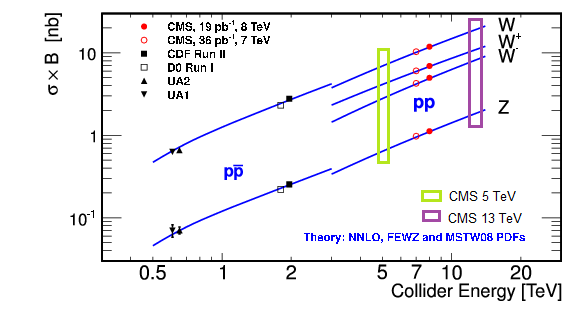
\includegraphics[width=0.6\linewidth]{plots/Intro/summary_v2.png}
%   \caption{1a}
%   \label{fig:Eff:el:5TeV:GSFSel:pos
\caption{Summary of previous measurements of the \W and \Z boson production cross section at hadron colliders. Not shown are the results from \sh LHC measurements. Measurements presented in this thesis are also indicated. Adapted from \cite{article_wzsummary}.}
\label{fig:intro:summary:meas}
\end{figure}

\section{Measuring the cross sections}
\subsubsection{\W and \Z decays}
\W and \Z bosons can decay both hadronically and leptonically. Branching fractions of the \W boson decay are $\sim67\%$ hadronic and $\sim33\%$ leptonic, and branching fractions of the \Z boson are $\sim70\%$ hadronic and $\sim10\%$ leptonic with the remaining $\sim 20\%$ being invisible decay channels\cite{PhysRevD.98.030001}. Lepton universality implies the leptonic decays are expected to occur at equal rates for each of the lepton flavors, $l=\mathrm{electrons}~ (e),~\mathrm{muons}~(\mu),~\mathrm{and~tau~leptons}~ (\tau)$. The \W and \Z boson leptonic decay channels are $\Z \to \ell^+ + \ell^-$ and $\W^{+(-)} \to \ell^{+(-)} +  \overset{\textbf{\fontsize{2pt}{2pt}\selectfont(---)}}{\nu_\ell}$, with $\ell=e,~\mu,~\tau$. These will henceforth be written as \zll and \wlnu (or with $\ell=e,~\mu,~\tau$), with charge and lepton number conservation laws implied.
Leptonic decay channels are utilized because electrons and muons can be reconstructed and identified well by CMS. A fairly clean sample and accurately modeled observables are important components of this measurement. The leptonic decays \zee and \zmm provide extremely clean signatures marked by the presence of a pair of oppositely charged same-flavor leptons. Similarly, the decay channels \wenu and \wmunu can be identified by the presence of a high-momentum electron or muon. 
\subsubsection{Cross section}
The cross section times branching ratio for a given channel is measured experimentally by determining the number of signal events observed and accounting for the acceptance of the measurement, as shown in Equation~\ref{eq:eq_xsec}. The acceptance of the fiducial volume is determined from simulation, and the efficiency scale factor is determined by measuring selection efficiency in both simulation and data. The following chapters of this thesis describe the derivation of these quantities in detail.
\begin{equation}\label{eq:eq_xsec}
\sigma\times Br = \frac{N_{sig}}{A\epsilon \int\mathcal{L} dt}
\end{equation}
\begin{itemize}
\item \nsig: Number of signal events observed in a given channel
\item $A$: The acceptance is the number of \W or \Z bosons producing a final state with leptons inside the fiducial measurement volume, divided by the total number of \W or \Z bosons produced. Determined from simulation. 
\item $\epsilon$: The efficiency scale factor, to account for the differences in rates of lepton identification and selection between simulation and data
\item $\int\mathcal{L}dt$: integrated luminosity. The integrated luminosity provides the number of $pp$ collisions measured in a given dataset.
\end{itemize}

\subsubsection{\Z boson cross section}
Measuring the cross section of the \Z boson is fairly straightforward, as the dilepton decay of a \Z boson is an extremely clean signature with minimal background. Two well-identified leptons, required to be of the same flavor be oppositely charged, within the invariant mass range \masswindow are taken to be candidates for \zll decays. Small background contributions primarily from diboson and \ttbar events are simulated, and the total contribution of the background processes is subtracted from the observed \Z boson yield. 

\subsubsection{\W boson cross section}
The \W boson decay channels used in this measurement include the production of a neutrino, which is not measured by CMS. Therefore, the final state cannot be fully reconstructed, and additionally has a fairly large background. Instead of a fully reconstructed final state, an observable, transverse missing energy, \met, is used to infer the momentum of the neutrino. Transverse mass, \mt, is constructed from the lepton momentum and \met as a proxy for the neutrino. The simulated \mt distribution for the \wlnu signal process, as well as several background processes, are used in a fit to data to determine the cross section. 
Measuring the \W boson production cross section relies on the \Z boson---there are multiple corrections that need to be derived for the \W boson simulations that cannot be done without the \Z boson. In addition to the lepton efficiency and momentum corrections, the fit to \mt requires an accurate modeling of \met and therefore the hadronic recoil in an event. Hadronic recoil corrections account for differences between simulation and data, and are derived in a data-driven approach which relies on the \Z boson, and are described in Chapter~\ref{ch:recoil}. 


\subsubsection{Measurements}
The results presented in this thesis are derived from datasets at \s = 5.02 \TeV and \s = 13 \TeV. This provides the opportunity to produce results with high precision for two center-of-mass energies. The measurements are presented as the cross sections for \Wp, \Wm, \W, \Z, as well as the ratios of the cross sections $W^+/W^-$, $W^+/Z$, $W^-/Z$, $W/Z$. Evaluating the ratios allows for the subtraction of any correlated systematic uncertainties, and increases the precision of the measurement. Notably, the uncertainty from the luminosity calibration is one of the largest uncertainties, and it completely cancels for these ratios. 
% Comment back in when I add the 13/5 ratios
% Additionally, making separate measurements at \s = 13 \TeV and \s = 5 \TeV provides another method for providing results with reduced uncertainties---taking ratios of the quantities: [13 \TeV]/[5 \TeV] allows us to further remove any correlated uncertainties. Some of the uncertainties which are correlated in this manner are the luminosity calibrations (partial correlation) and the theoretical uncertainties on the predictions. 


\section{Impact of the Measurement}
\W and \Z boson production is an important measurement at any hadron collider. The precision measurement of the \W and \Z boson production provides a precision test of the Standard Model (SM), as well as a benchmark for the state-of-the-art calculations and models that are used to describe the proton and simulate physical interactions at the LHC and other experiments. The inclusive cross section measurements are the foundation of differential cross section measurements which provide greater constraints on different aspects of the models.  \W and \Z boson production is also significant background to many other electroweak measurements and searches for new physics.
Additionally, \W and \Z bosons are a significant source of isolated, high-\pt leptons. The clean signature of \zll is used for detector calibration and luminosity monitoring \cite{xinmei}.

\chapter{Physics Background}\label{ch:sm}
The Standard Model of particle physics is a $SU(3)\otimes SU(2)\otimes U(1)$ gauge theory that describes the interactions of fundamental particles. It is generally described in two parts, electroweak theory and quantum chromodynamics, presented in the following section. In later sections, the production of \W and \Z bosons in \pp collisions and the modeling of these processes is described. 


%%%%%%%%%%%%%%%%%%%%%%%%%%%%%%%%%%%%%%%%%%%%%%%%%%
%               Standard Model
%%%%%%%%%%%%%%%%%%%%%%%%%%%%%%%%%%%%%%%%%%%%%%%%%%

\section{The Standard Model}\label{ch:sm:sm}
\subsubsection{Introduction}
The SM has been a remarkably successful theory describing fundamental particles and their interactions. The fundamental constituents of matter---leptons and quarks---interact through the strong and electroweak interactions. Depicted in Figure~\ref{fig:intro:sm}, the SM consists of three families of quarks (purple), three families of leptons (green), the force carriers (red), and the Higgs boson (yellow). 

\begin{figure}
\centering
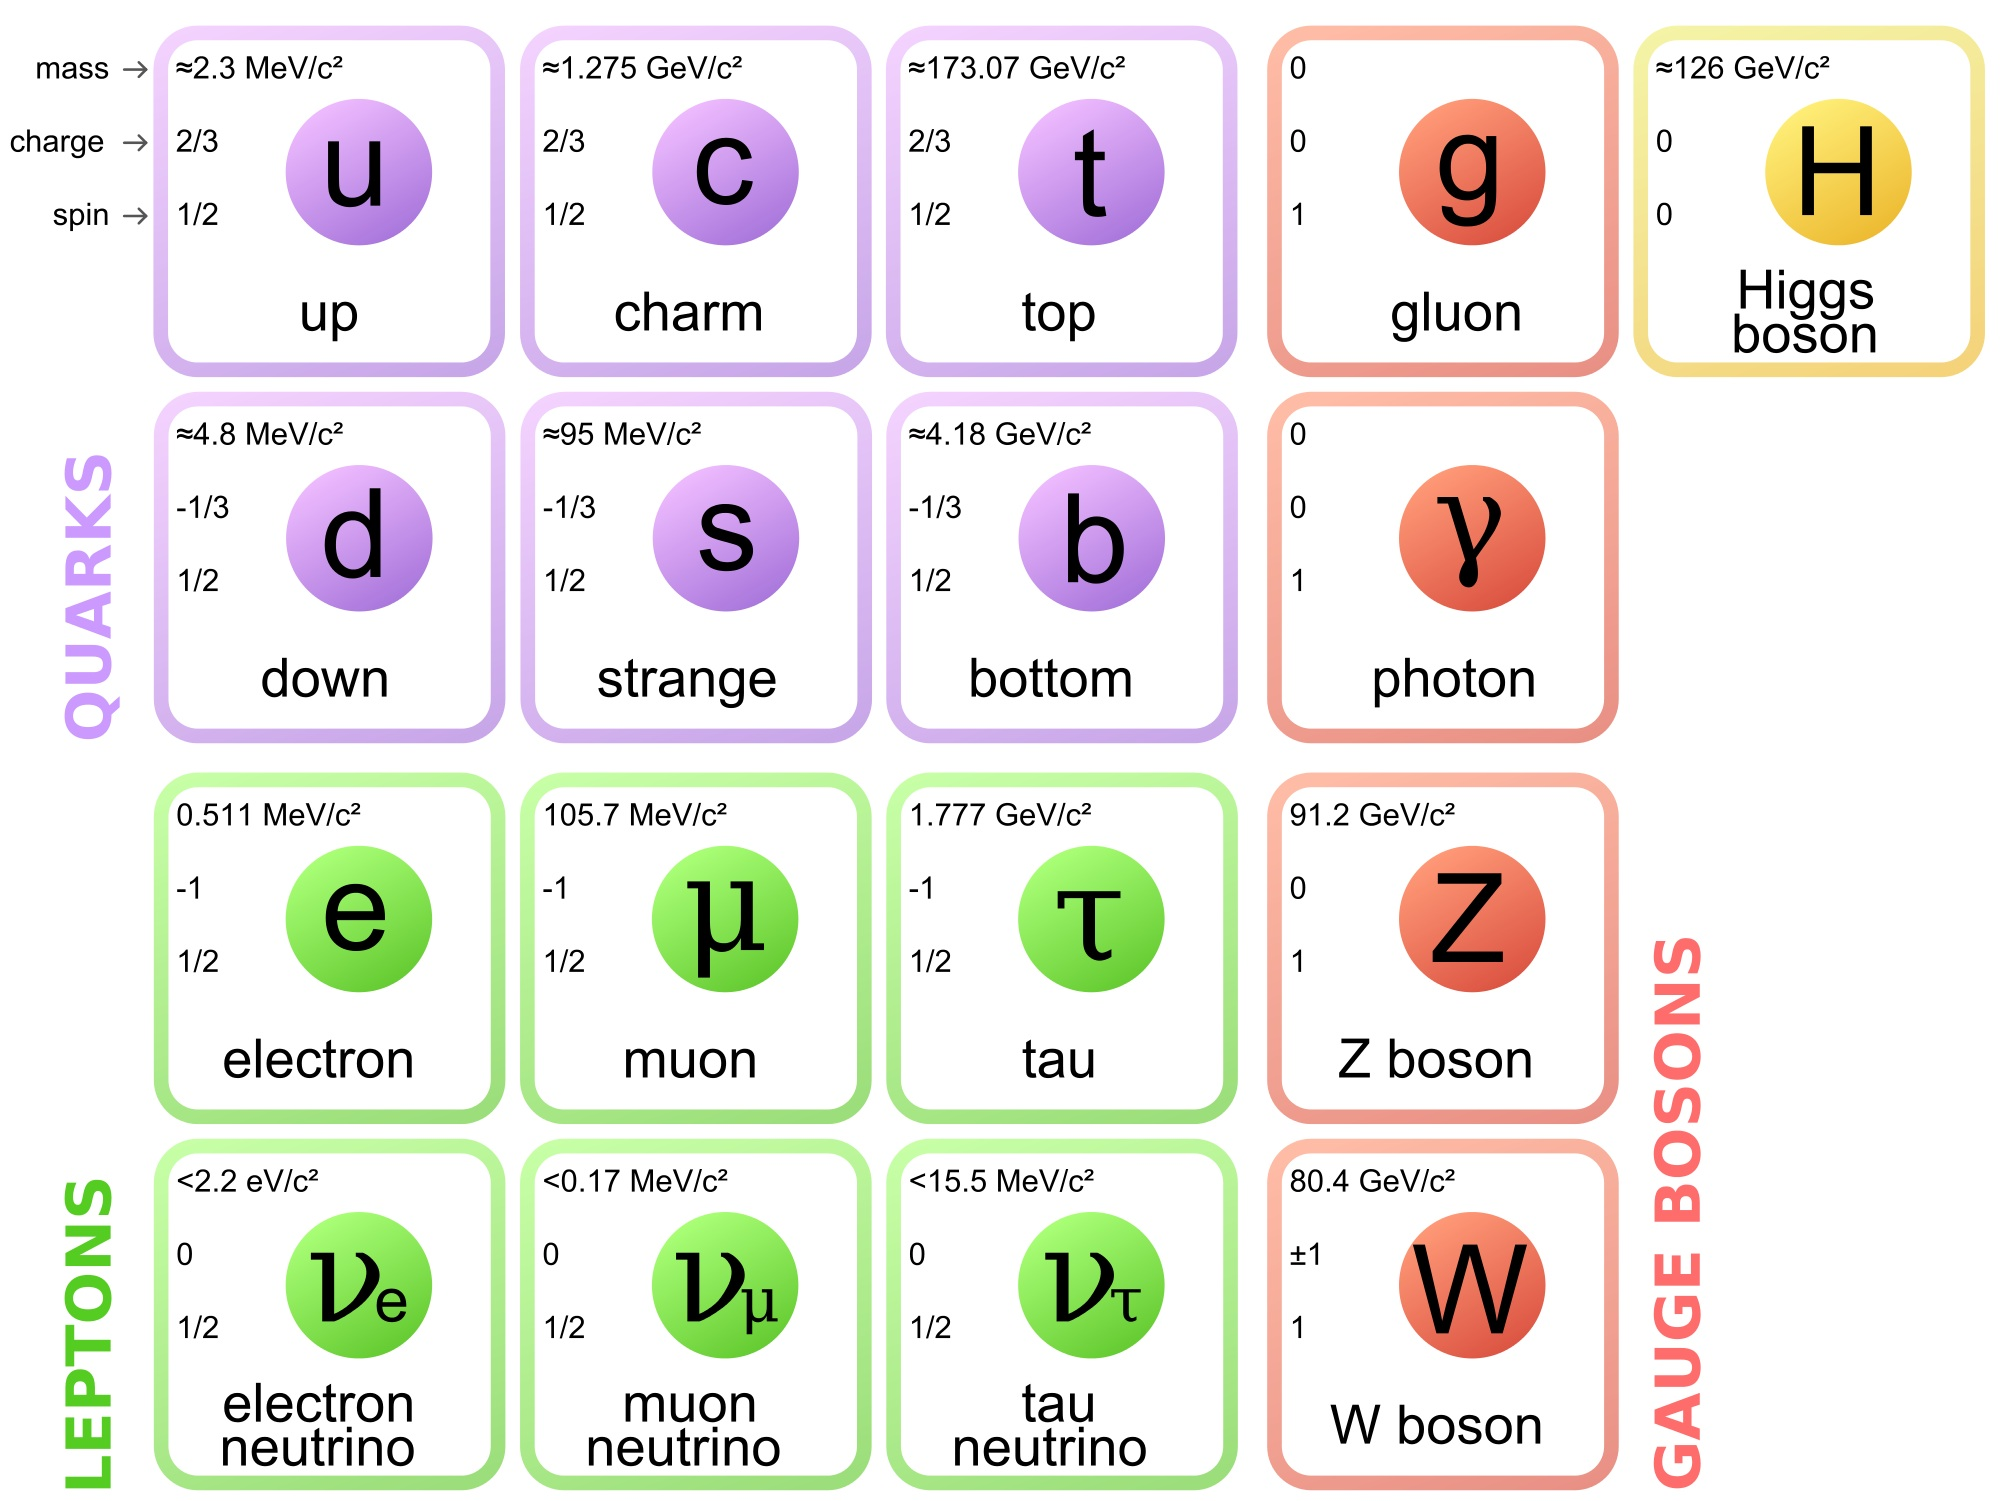
\includegraphics[width=0.6\linewidth]{plots/Intro/sm.jpg}
%   \caption{1a}
%   \label{fig:Eff:el:5TeV:GSFSel:pos
\caption{Fundamental particles of the Standard Model\cite{SM_table}.} \label{fig:intro:sm}
\end{figure}

Familiar building blocks of matter---protons and neutrons---are not the most basic particles, they are composed of constituent quarks and gluons. There are three families of quarks, with six total flavors. Up-type quarks up ($u$), charm ($c$), and top ($t$) have electric charge $+\frac{2}{3} e$, and down-type quarks down ($d$), strange ($s$), and bottom ($b$) have electric charge $-\frac{1}{3}e$. Protons are $uud$, with an electric charge of $+1e$. The strong interaction, mediated by the gluon, binds quarks together into hadrons. The strength of the strong coupling is distance-dependent, with coupling increasing\phil{decreasing or strong coupling at short scales} at long length scales. Therefore, bare quarks have never been observed, as it is favored for them to quickly form bound states. The lepton families are the electron and its more massive analogs, the muon and tau leptons, along with their corresponding neutrinos. 

The weak interaction is propagated by the \W and \Z bosons. Both the charged leptons, neutrinos, and quarks can couple to \W and \Z bosons.  At low energies, the weak interaction is commonly know for its role in beta decay, with uses such as radioluminescent tritium illumination sources and medical imaging positron emission tomography (PET scan).  At energies achieved by the LHC, the \W and \Z bosons can be produced in $pp$ collisions and the properties of the production can be studied. As described in below, this provides important information on several fronts, including event modeling and detector performance.


%%%%%%%%%%%%%%%%%%%%%%%%%%%%%%%%%%%%%%%%%%%%%%%%%%
%                     ewk
%%%%%%%%%%%%%%%%%%%%%%%%%%%%%%%%%%%%%%%%%%%%%%%%%%

\subsection{Electroweak Theory}\label{ch:sm:ewk}
In the SM\cite{SMEWK1,SMEWK2,SMEWK3}, electroweak interactions belong to the gauge group $SU(2) \otimes U(1)$, with the gauge bosons $W_{\mu}^i$ ($i = 1,2,3$) for $SU(2)$ and  $B_{\mu}$ for $U(1)$.  The left-handed fermions transform as doublets, where the leptons are given in Equation~\ref{eq:phys:ewk:leptons} and quarks are shown in Equation~\ref{eq:phys:ewk:quarks}. The $d_i'$ are given by $d_i' = \sum_j V_{ij} d_i$, where $V_{ij}$ are the elements of the Cabibbo-Kobayashi-Maskawa (CKM) matrix\cite{ckm1,ckm2}.
\begin{equation}
  \Psi=\binom{v_e}{l_e},~\binom{v_{\mu}}{l_{\mu}},~\binom{v_{\tau}}{l_{\tau}}
  \label{eq:phys:ewk:leptons}
\end{equation}
\begin{equation}
  \Psi=\binom{u}{d'},~\binom{c}{s'},~\binom{t}{b'}
  \label{eq:phys:ewk:quarks}
\end{equation}
Vector fields corresponding to particles with spin 1 and mass are the $W_\mu^\pm$, $Z_\mu$, and photon $A_\mu$, which are given in terms of the gauge fields as:
\begin{equation}
\begin{aligned}
    &A_\mu = B\mu cos\theta + W^3_\mu sin\theta\\
&Z_\mu = -B\mu sin\theta + W^3_\mu sin\theta\\
&W_\mu^\pm = W_\mu^1 \mp i W^2_\mu
\end{aligned}
\label{eq:ewk_s1_particles}
\end{equation}

Mass generation is achieved through spontaneous symmetry breaking of $SU(2)\otimes U(1)$ to $U(1)_{em}$ with the addition of a complex scalar doublet $\phi = \frac{1}{\sqrt{2}}\binom{\sqrt{2}\phi^+}{\phi^0 + ia^0}$, known as the Brout-Englert-Higgs mechanism\cite{ewsb1,ewsb2,ewsb3}. The potential is given by $V(\phi) = \mu^2\phi^\dagger\phi + \lambda^2(\phi^\dagger \phi)^2$, with the full Lagrangian being given in Equation~\ref{eq:lagrangian_higgs}. With $\mu^2 < 0$, the vacuum expectation value of $\phi$ is $<\phi> = v/\sqrt{2} = \mu/\lambda$ with $v\approx 246$ GeV. 
\phil{I would call below $\mathcal{L_{Higgs}}$}

\begin{equation}
    \mathcal{L} = (D_\mu\Phi)^\dagger(D^\mu\Phi) - \mu^2 \Phi^\dagger\Phi - \lambda(\Phi^\dagger\Phi)^2
    \label{eq:lagrangian_higgs}
\end{equation}
The covariant derivatives of Equation~\ref{eq:lagrangian_higgs}, $D_\mu\Phi$, provide the couplings between the Higgs fields and the $W_\mu$ and $B_\mu$ gauge fields, shown in Equation~\ref{eq:covariant_deriv}
\begin{equation}
    D_\mu \Phi = (\partial_\mu + ig\sigma^aW_\mu^a/2 + ig'YB_\mu/2)\Phi
    \label{eq:covariant_deriv}
\end{equation}
Three of the four degrees of freedom introduced by the Higgs doublet are absorbed into the $W^i_\mu$ and $B_\mu$ fields of the $SU(2)\otimes U(1)$ and become the longitudinal components of the \W and \Z bosons. The physical \W and \Z bosons also acquire mass. The generator of the unbroken $U(1)_{em}$ gauge symmetry, the photon, remains massless. The remaining degree of freedom manifests as the new neutral scalar particle, the Higgs boson. The masses of the physical bosons are given in Equation~\ref{eq:boson_masses}.
\begin{equation}
\begin{aligned}
m_H &= \lambda v \\ 
m_W &= \frac{1}{2}g v = cos\theta_W m_Z \\ 
m_z &= \frac{1}{2}\sqrt{g^2+g'^2}v  = \frac{M_W}{\cos{\theta_W}}\\ 
m_\gamma &= 0
\end{aligned}
\label{eq:boson_masses}
\end{equation}
Fermion masses are likewise given through a Yukawa coupling to the Higgs field, shown in Equation~\ref{eq:yukawa}. Fermion masses become $m_{f_i} = h_{f_i} v / \sqrt{2}$ after rotation into a basis where the Higgs-fermion interaction is diagonalized. The fermion coupling to the Higgs boson is $\frac{m_f}{v}\bar{f}fH$, proportional to its mass.
\begin{equation}
\mathcal{L}_{yukawa} = -\hat{h}_{d_{i,j}}\bar{q}_{L_i}\Phi d_{R_j} - \hat{h}_{u_{i,j}}\bar{q}_{L_i}\bar{\Phi} u_{R_j} -\hat{h}_{l_{i,j}}\bar{l}_{L_i}\Phi e_{R_j} + h.c.
    \label{eq:yukawa}
\end{equation}
In Equation~\ref{eq:yukawa}, $q_L$ and $u_R,d_R$ are the quark doubles and singlets, and $l_L$ and $e_R$ are the lepton doublets and singlets. As the Higgs boson is electromagnetically neutral and also transforms as a singlet in $SU(3)$, there are no tree-level couplings of the Higgs to either photons or gluons.

%%%%%%%%%%%%%%%%%%%%%%%%%%%%%%%%%%%%%%%%%%%%%%%%%%
%                     qcd
%%%%%%%%%%%%%%%%%%%%%%%%%%%%%%%%%%%%%%%%%%%%%%%%%%

\subsection{Quantum Chromodynamics}\label{ch:sm:qcd}

The strong interaction between quarks and gluons is described by quantum chromodynamics (QCD), the $SU(3)$ part of the SM. Interactions between quarks and gluons is described by the Dirac Lagrangian density given in Equation~\ref{eq:qcd_lagrangian}. Quarks and gluons carry color charges (red, green, or blue: $N_C = 3$), and there are eight color-combinations of gluons as mediators of the strong force ($A^C_\mu$,~$C=[1...8]$). Quarks are represented by the $\bar{\psi}_{f,\alpha}$ spinors, with the six flavors of quarks ($u,c,t,d,s,b$) represented by $f$, the three colors by $\alpha$, and the quark masses by $m_f$.
\phil{You forgot $\psi$ ie $\gamma_{f,\beta}\psi_{f,\alpha}$}

%% QCD Lagrangian
\begin{equation}
    \mathcal{L}=\bar{\psi}_{f,\alpha}(i\gamma^\mu \partial_\mu \delta_{\alpha\beta}-g_s\gamma^\mu t^C_{\alpha\beta}\mathcal{A}^C_\mu-m_f\delta_{\alpha\beta})\gamma_{f,\beta}-\frac{1}{4}F^b_{\mu\nu}F^{b,\mu\nu}
    \label{eq:qcd_lagrangian}
\end{equation}
%% %% Full Lagrangian
% \begin{equation}
%     \mathcal{L}=\bar{\psi}_{f,\alpha}(i\gamma^\mu \partial_\mu \delta_{\alpha\beta}-g_s\gamma^\mu t^C_{\alpha\beta}\mathcal{A}^C_\mu-m_f\delta_{\alpha\beta})\gamma_{f,\beta}-\frac{1}{4}F^b_{\mu\nu}F^{b,\mu\nu}-\theta\frac{g^2_{s}}{72\pi^2}\epsilon_{\mu\nu\rho\sigma}F^{c,\mu\nu}F^{c,\rho\sigma}
%     \label{eq:qcd_lagrangian}
% \end{equation}
 The eight generators of the $SU(3)$ color group are $3\times 3$ matrices $t^C_{\alpha\beta}$. The strong coupling constant is $g_s$ ($\sqrt{4\pi\alpha_s}$), where $\alpha_s$ varies with energy scale.  The gluon field tensors $F_{\mu\nu}$ are shown in Equation~\ref{eq:qcd_field_tensors}, where the $f_{ABC}$ are the structure constants of $SU(3)$.
\begin{equation}
F_{\mu\nu}^A = \delta_{\mu} \mathcal{A}^A_{\nu} - \delta_{\nu} \mathcal{A}^A_\mu - g_s f_{ABC} \mathcal{A}_\mu^B \mathcal{A}_\nu^C,~~~~ [t^A, t^B] = if_{ABC}t^C
\label{eq:qcd_field_tensors}
\end{equation}
The parameters of QCD are the quark masses ($m_f$) and the coupling constant ($g_s$). There is an additional term in the QCD Lagrangian which is not included in Equation~\ref{eq:qcd_lagrangian}, which contains a parameter $\theta$, and allows for CP violation in QCD. Experimental limits on the neutron electric dipole moment constrain this term to be $\theta < 10^{-10}$ \cite{PhysRevLett.97.131801}.

Computational methods for QCD predictions include lattice gauge theory and perturbative expansion methods. Feynman rules for QCD allow diagrams with $q\bar{q}g$ and $ggg$ vertices and a $gggg$ vertex\cite{Ellis:1991qj}. Perturbative QCD (pQCD) expresses predictions for observables as an expansion in terms of the coupling $\alpha_s(\mu_R^2)$ i.e. $f = f_0 + f_1\alpha_s + f_2\alpha_s^2 + f_3\alpha_s^3 +....$. The coupling $\alpha_s(\mu_R^2)$ is a function of the renormalization scale $\mu_R$, and the effective strength of the interaction with momentum transfer $Q^2$ is $\alpha_s(\mu_R^2 \sim Q^2)$. Calculations are done with Feynman diagrams and are generally performed to only a few terms---leading order (LO, first term), next-to-leading order (NLO, first two terms), and so forth.
The scale dependence of QCD is expressed in the renormalization group equation:
\begin{equation}
    \mu^2_R\frac{d\alpha_s}{d\mu_R^2} = \beta(\alpha_s) = -(b_0 \alpha_s^2 + b_1 \alpha_s^3 + b_2 \alpha_s^4 + \cdots)
    \label{eq:renormalization_group}
\end{equation}
%where $b_0$ is the 1-loop coefficient, $b_1$ is the 2-loop coefficient, etc. 
The minus sign indicates that the coupling becomes weak for interactions with high momentum transfer and is strongly interacting for low energy scales, the source of asymptotic freedom \cite{PhysRevLett.30.1346, PhysRevLett.30.1343}. Values of $\alpha_s$ range from $\alpha_s \sim 0.1$ for $Q$ in the $100 \GeV - \TeV$ range to over $\alpha_s \sim 0.3$ for processes with momentum transfer $Q \sim 1 \GeV$, as depicted in Figure~\ref{fig:sm:alpha_s}. Free quarks have not been observed---they quickly hadronize into mesons or baryons on the time scale $\sim 1/\Lambda$, while the top quark decays before hadronization. This is understood as a result of the strong coupling increasing at low energies (large distance scales), and only the color-singlet hadrons are observed.
\begin{figure}[htbp]
\centering
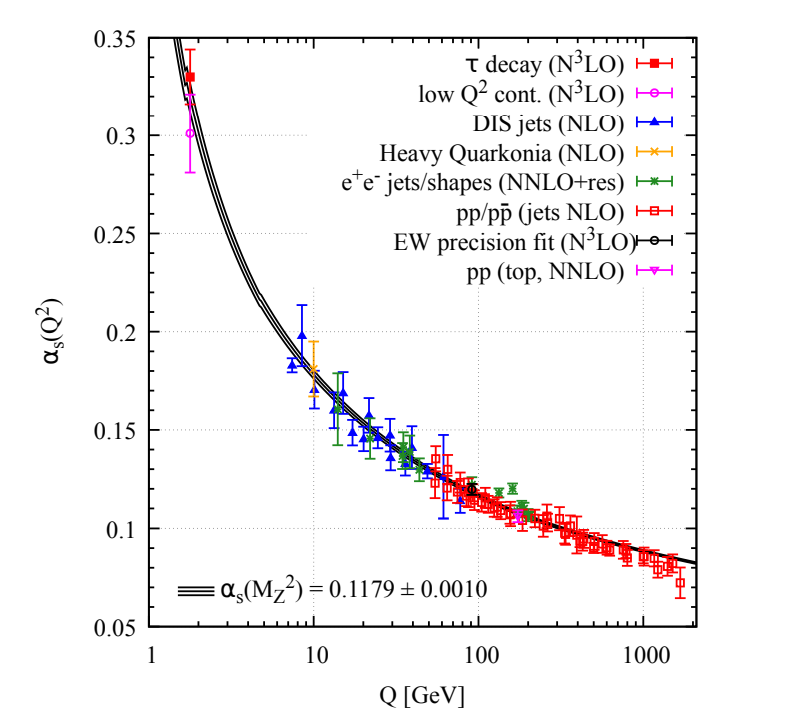
\includegraphics[width=0.6\linewidth]{plots/SM/a_s.png}
\caption{Measurements of $\alpha_s$ demonstrating the scale-dependence\cite{PhysRevD.98.030001}.}
\label{fig:sm:alpha_s}
\end{figure}
\section{Modeling \pp collisions}
In collisions at very low energies, protons can be approximated as electrically charged objects. At higher energies, such as those at the LHC, the structure within protons begins to have an important role for the scattering process. \W and \Z bosons are produced from the interaction of quarks and gluons (both also referred to as partons) within the proton\cite{PhysRevLett.23.930,PhysRevLett.23.935}. The contributions of the partons to the proton's structure are described by parton distribution functions (PDFs). The PDFs cannot be calculated directly, and are instead determined from experimental data.  (add citations) Valence quarks, sea quarks, and gluons within the proton are described by the PDFs. 
% Therefore, the internal structure of the protons is represented by the structure functions i.e. in Equation~\ref{eq:structure_func}, where the $x$ is the fraction of the proton's total momentum carried by a given parton, and $f_i(x)$ is the distribution of the parton. 
% \begin{equation}
% F(x) = \sum_i{x_if_i(x_i)}
    % \label{eq:structure_func}
% \end{equation}

Calculations for cross section predictions must be done perturabitively in QCD. The highest order calculation currently available for the \W and \Z production is NNLO
\cite{Anastasiou:2003ds}. However, soft and collinear gluons emissions produce logarithmic terms which cause singularities. The factorization theorem can be used in QCD processes, separating the perturbative and non-perturbative sections of the calculation at a factorization scale, $\mu_F$~\cite{Collins:1989gx}. This allows the singularities due to the soft gluon emissions to be factored out and contained within the PDFs.  Equation~\ref{eq:factorization_xsec} shows the factorized cross section calculation. $f_{a}$ and $f_{b}$ are the parton distribution functions for the quarks and gluons in the two protons, $x_a$ and $x_b$ are the fractions of total momentum carried by each parton, and $\hat{\sigma}$ is the cross section for the hard process. 

\begin{equation}
\begin{aligned}
\sigma_{p_a p_b \rightarrow n} &= \sum_{a,b}{\int{dx_a dx_b f_{a}(x_a, \mu^2_F)f_{b}(x_b, \mu^2_F)}} \\ &\times[\hat{\sigma}_{LO}(x_a x_b s, \mu^2_R, \mu^2_F)+\alpha_S \hat{\sigma}_{NLO}(x_a x_b s, \mu^2_R, \mu^2_F) + \cdot]
    \label{eq:factorization_xsec}
\end{aligned}
\end{equation}
Factorization scale dependence of the PDFs is determined by the DGLAP equation. Parametrizations of PDFs are determined, and solutions to the DGLAP equation provide the evolution of the PDFs over different scales of $\mu_F$ \cite{Gribov:1972ri,Dokshitzer:1977sg}

\begin{figure}
\centering
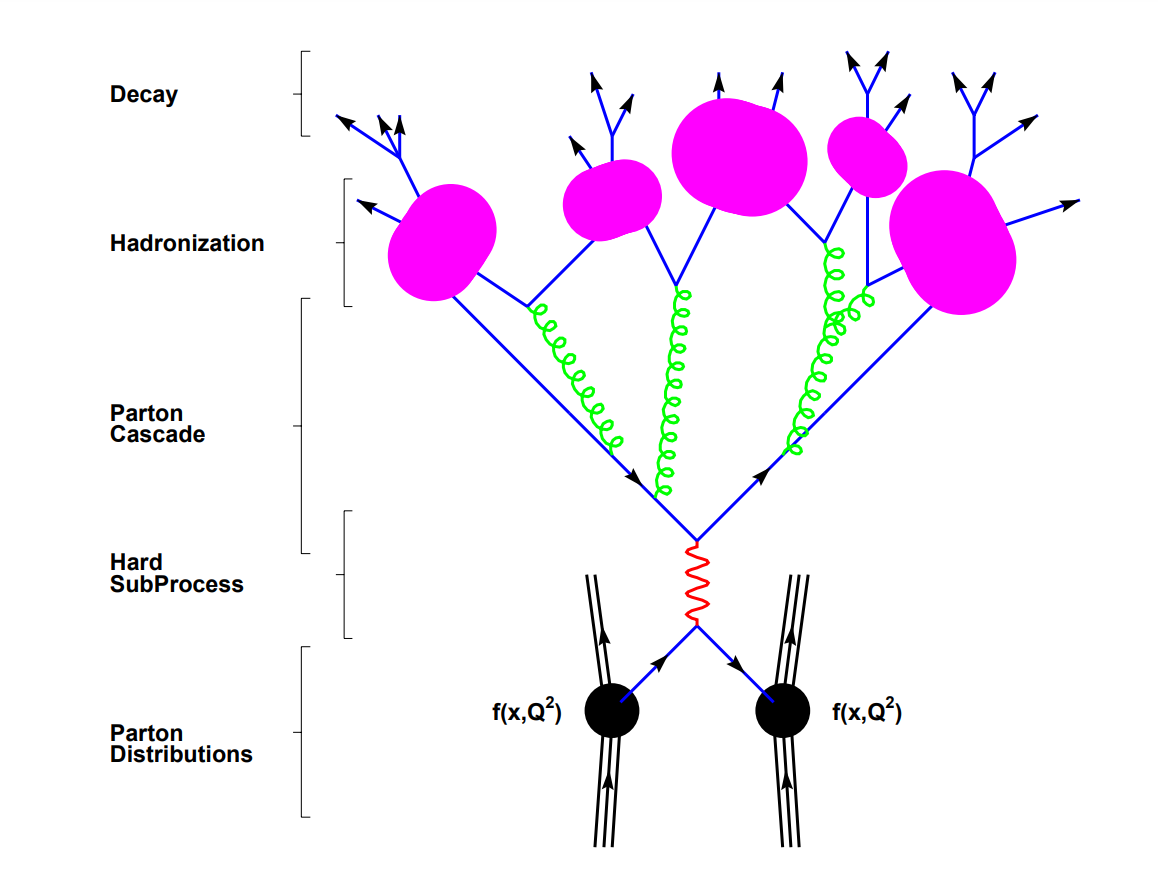
\includegraphics[width=0.6\linewidth]{plots/SM/evtgenerator.PNG}
%   \caption{1a}
%   \label{fig:Eff:el:5TeV:GSFSel:pos
\caption{Illustration of a hard-scatter process. \protect\cite{Dobbs:2001ck}}
\label{fig:sm:evtgen}
\end{figure}

Matrix element calculation breaks down for soft and collinear final states. Instead, parton shower models are used to produce the final-states at non-perturbative scales. Showering is modeled as series of radiative steps, with partons branching into consecutively lower energy state: $q\rightarrow gq$, $g\rightarrow gg$, and $g\rightarrow q\bar{q}$ for QCD. Additionally QED interactions ($q\rightarrow q\gamma$ and $l\rightarrow l\gamma$) are included in the shower modeling. Parton showering continues to the scale $\Lambda_{QCD}\approx 200~\mathrm{MeV}$, bare partons are hadronized into color-neutral hadrons. Then the unstable hadrons are decayed according to branching ratios. Factorization and a hard scatter process, along with subsequent parton showering and hadronization is illustrated in Figure~\ref{fig:sm:evtgen}.



\subsection{\W and \Z production at the LHC [need some work]}
In the \pp collisions, the bosons are produced through the interaction of quarks and gluons within the protons \cite{}. The primary production modes for the \W and \Z bosons is through the Drell-Yann process, predonminantly $u\bar{u}, d\bar{d}\rightarrow Z$,  $u\bar{d}\rightarrow W^+$,  and $d\bar{u}\rightarrow W^-$. 

Figure~\ref{fig:sm:summary:xVsQ2}.

%%%% figure
\begin{figure}
\centering
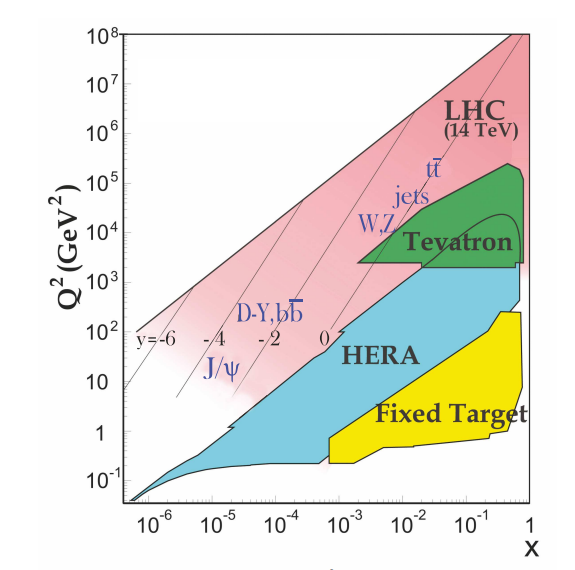
\includegraphics[width=0.6\linewidth]{plots/SM/structure_probes.PNG}
%   \caption{1a}
%   \label{fig:Eff:el:5TeV:GSFSel:pos
\caption{Phase space of Bjorken-x and $Q^2$ available at the LHC and other experiments. \pp collisions at the LHC can probe very high $Q^2$. \protect\cite{PhysRevD.98.030001}}
\label{fig:sm:summary:xVsQ2}
\end{figure}



% \subsection{Simulating \pp collisions[need some work]}
% Practical descriptions of theoretical predictions are provided by Monte Carlo event generators. These generators rely on the approximations and factorization schemes that were described earlier in this section. Many collaborations dedicated to event generation tools exist, and are important in the era of LHC physics. The event generators come in generally two types: matrix element generators and parton shower generators. The matrix-element generators are distinguished by the order in $\alpha_s$ to which they provide calculations. 
% \begin{itemize}
%     \item \textbf{Pythia}: Pythia is a general-purpose event generator and can do both matrix-element calculation as well as initial and final state radiation and multiparton interactions. Pythia is often interfaced to other matrix-element calculators, where it provides the parton showering and hadronization steps, as done for the samples used in this analysis. \cite{Sjostrand:2014zea}
%     \item \textbf{aMC@NLO} MadGraph5\_aMC@NLO is a generator which provides matrix element calculations with up to two additional partons in the final state. This uses the NNPDF3.1 NLO PDF set.
%     \item \textbf{ResBos} 
%     \item \textbf{Powheg}
% \end{itemize}


% Predictions from event generators have uncertainties from several sources. Low-energy QCD processes which are dominiated by non-perturabtive effects are not well modeled and have large uncertainties. Parton showering is limited by its reliance on approximations. Proton PDFs have uncertainties. Additional uncertainty comes from higher-order terms in both QCD and QED, which are currently used at NNLO and LO. 

% PDF  uncertainties - general comment
% include multiple error sets reflecting the best fit with 1 sigma variations on the all of the params in the fit
% reflect uncertainties in data also
% inherent systematics dependent on way global fit is set up


% better predicionts of ewk mixing angle, w mass etc

\chapter{The CMS Experiment at the LHC}\label{ch:exp}
This measurement was performed using data collected by the Compact Muon Solenoid (CMS) Experiment, one of the multipurpose detector experiments at the LHC. This chapter details the technical design and operation of the LHC and CMS. 

%%%%%%%%%%%%%%%%%%%%%%%%%%%%%%%%%%%%%%%%%%%%%%
%            LHC 
%%%%%%%%%%%%%%%%%%%%%%%%%%%%%%%%%%%%%%%%%%%%%%

\section{The Large Hadron Collider}
The Large Hadron Collider is an 26.7 km-circumference accelerator designed to circulate protons or heavy nuclei in opposing directions and collide the\phil{reword sentence} complex designed to collide opposing proton beams at a center-of-mass energy of up to $\sqrt{s}=14\mathrm{TeV}$. It is housed in an underground tunnel with a circumference of 26.7 km, crossing the French-Swiss border, at a depth between 40m to 170m. This tunnel was previously home to the electron-positron collider, LEP. In addition to providing proton beams, the LHC is also capable of circulating lead nuclei at an energy of 2.3 TeV per nucleus beam. The LHC and accelerator complex at CERN are shown in Figure~\ref{fig:cern_accel_cartoon}.
%insert figure. 
% add figure
\begin{figure}
\centering
  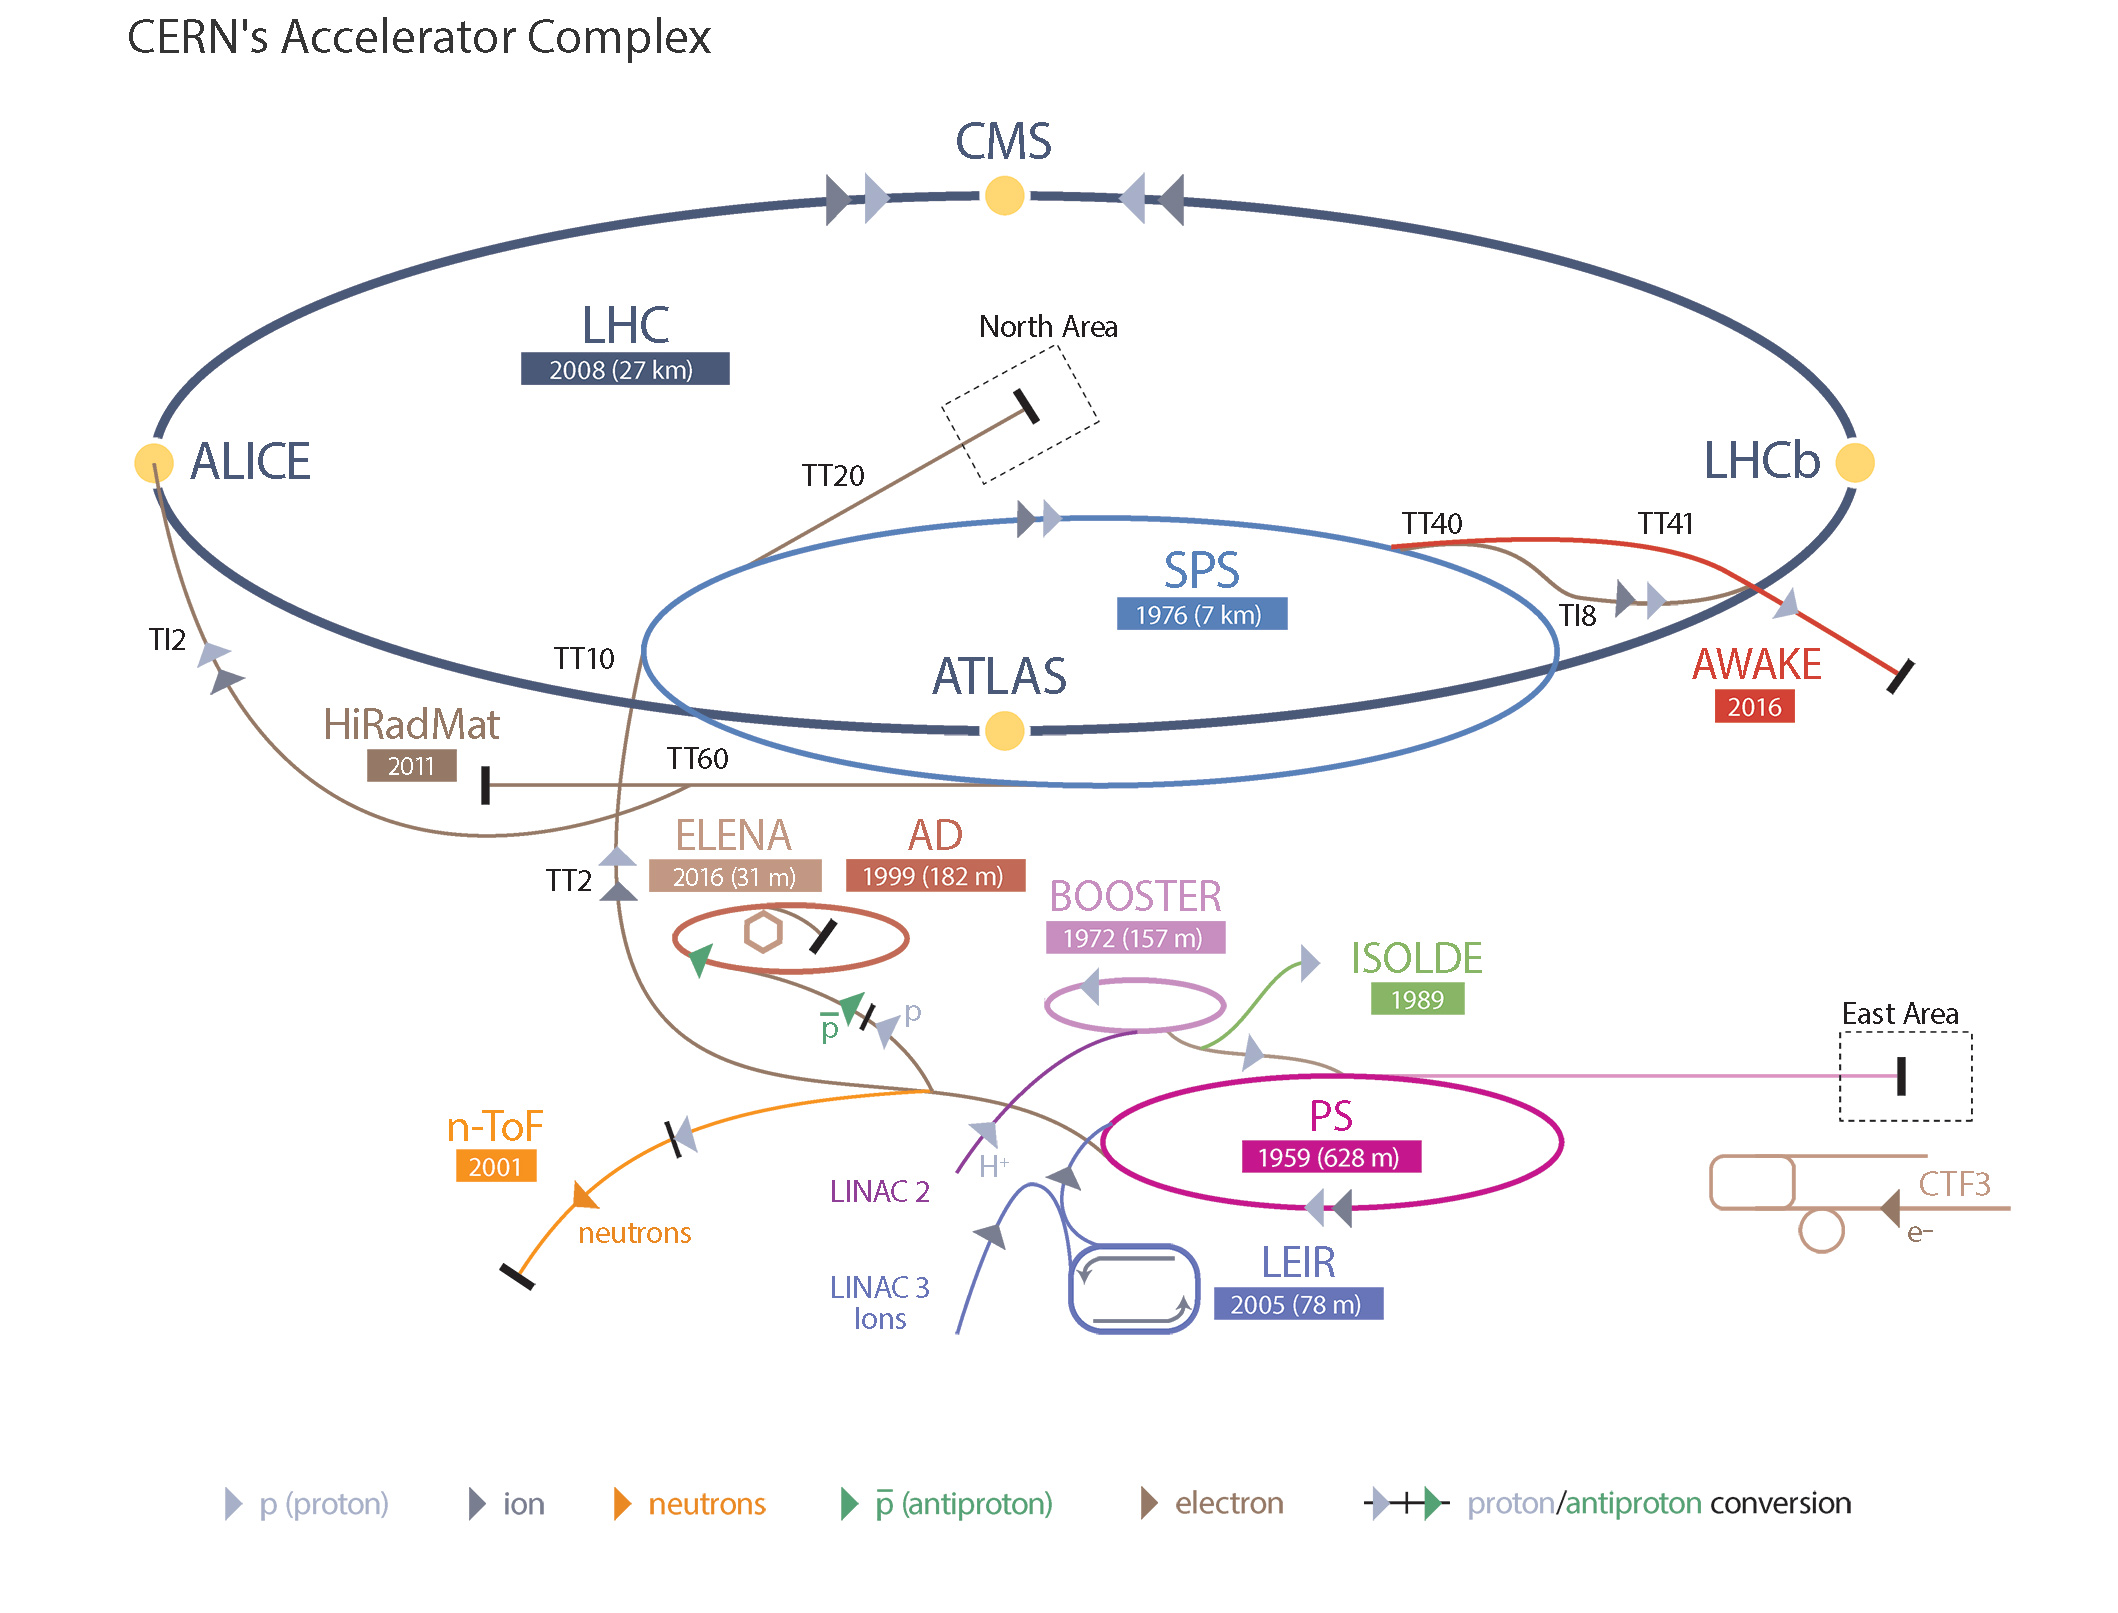
\includegraphics[width=0.75\linewidth]{plots/LHC/CERN_accelerators.jpg} %% put in this figure
  %https://cds.cern.ch/record/40524
  \caption{Illustration of the full accelerator complex at CERN, including the pre-accelerators, the LHC, and the major collision halls at the LHC.  \protect\cite{LHC_Accel_Cartoon}}
  \label{fig:cern_accel_cartoon}
\end{figure}

%%%%%%%% Producing Protons & pre-accelerator 
\subsubsection{LHC Pre-Accelerators}
Protons are produced by ionizing hydrogen gas, which are accelerated to 50 MeV by LINAC2, and injected into the Proton Synchroton Booster. The PSB then brings the protons to 1.6 GeV for injection into the Proton Synchrotron (PS). The PS takes six proton bunches, splits each into three prior to acceleration to 25 GeV, then subsequently splits each bunch into four prior to injection into the Super Proton Synchroton (SPS), resulting in 72 bunches injected into the SPS. The SPS can receive up to 4 sets of 72 bunches from the PS, accelerating them to 450 GeV per proton for injection into the LHC where they are further accelerated to a maximum of 6.5 GeV per proton. Bunches from SPS can be injected into the LHC up to 24 times, for a minimum spacing of 25 ns between bunch crossings\cite{Benedikt:2004wm}. 

\subsubsection{The Large Hadron Collider}
After injection into the LHC, protons are accelerated by radio-frequency (RF) cavities to an energy of 6.5 TeV. 
The trajectory of the protons around the ring is controlled by 1232 niobium-titanium wire superconducting dipole magnets, 15m in length, which are cooled by liquid Helium to a temperature of 1.9 K and have a magnetic field strength of 8.33 T. These dipole magnets are responsible for bending the proton beams in the appropriate direction around the LHC. Superconducting quadrupole magnets, 5-7 m in length, are used to focus the proton bunches.  The focusing quadrupoles are located near the collision points, to produce a more tightly spaced beam in preparation for collisions. Higher-order multipole magnets are also used for beam focusing and control. 
The beams circulated in the LHC are proton-proton, so the same beampipe cannot be used for both beams. Therefore a twin-bore magnet design is employed, where both beampipes are situated on the interior of the same magnet. A cross-section of an LHC dipole is shown in Figure \ref{fig:lhc_dipole} \cite{Bruning:2004ej}.
% add figure
\begin{figure}
\centering
  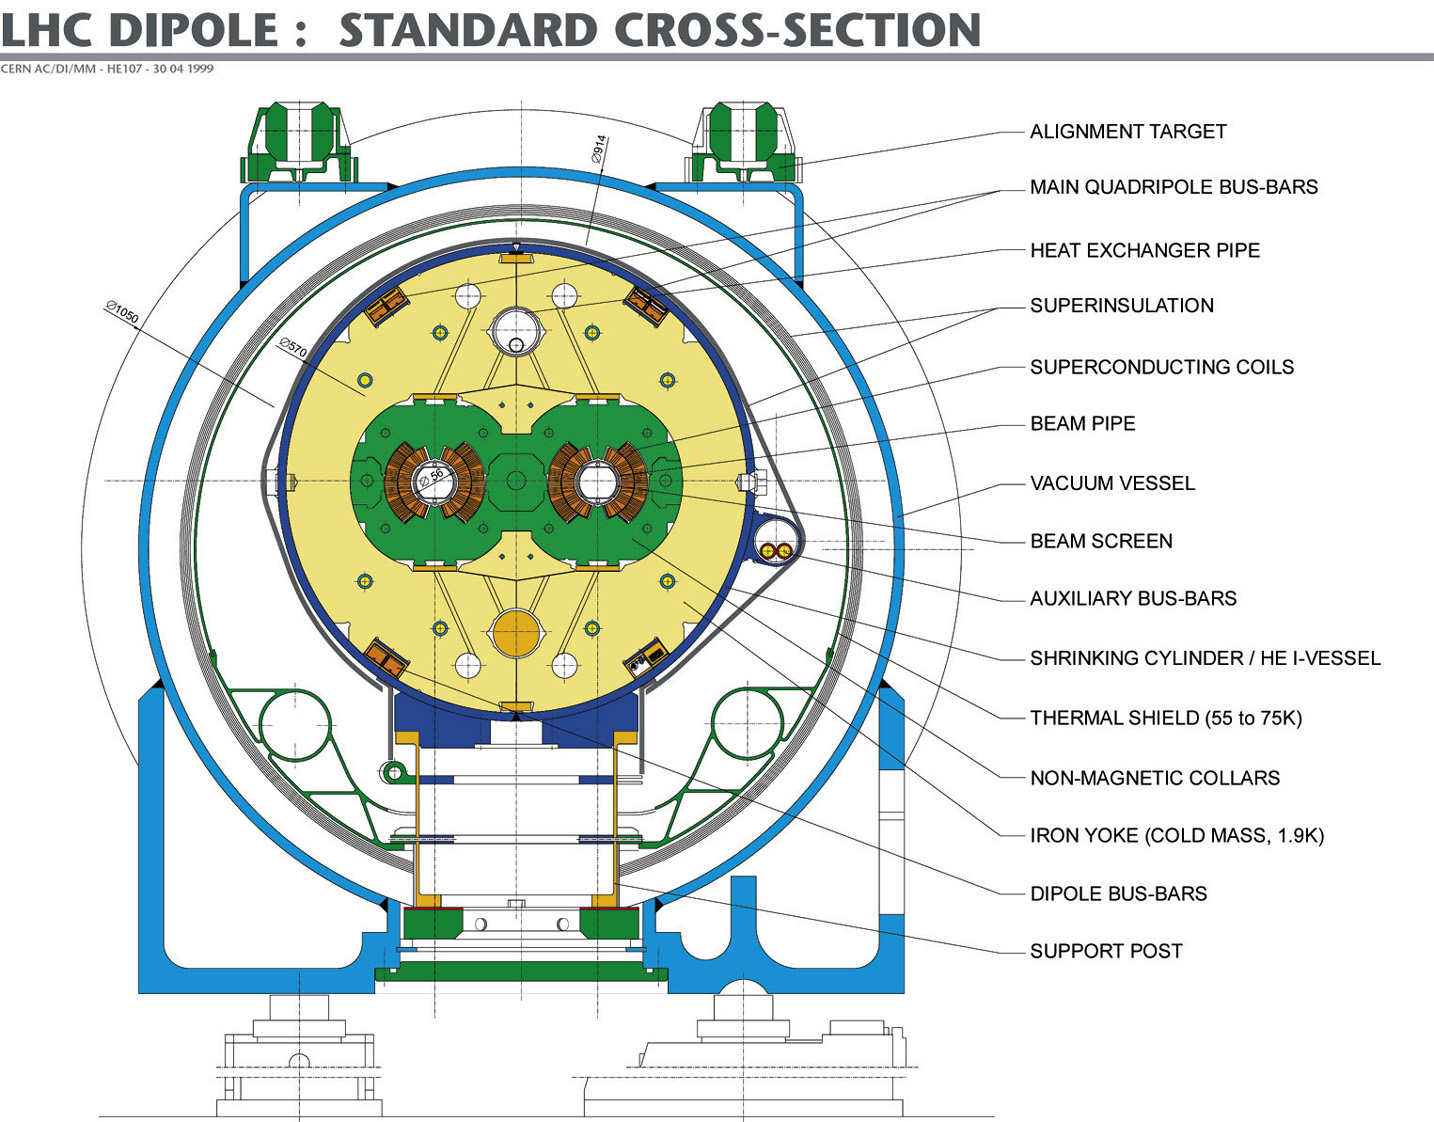
\includegraphics[width=0.5\linewidth]{plots/LHC/LHC_dipole.jpeg} %% put in this figure
  %https://cds.cern.ch/record/40524
  \caption{Cross-section of an LHC dipole magnet, showing the twin-bore design to accomodate the beampipes. \protect\cite{Team:40524}}
  \label{fig:lhc_dipole}
\end{figure}

Collisions occur where the beams intersect each other, located at multiple points around the LHC: Point 1 (ATLAS), Point 2 (ALICE), Point 5 (CMS), and Point 8 (LHCb). 
\section{The Compact Muon Solenoid}\label{ch:cms:CMS}

Data used in this thesis were collected by the CMS experiment. CMS is situated at LHC collision Point 5 near Cessy, France, and is depicted in Figure~\ref{fig:cms:cms_full}. CMS was designed for highly performant reconstruction of muons over a wide momentum range, high resolution tracking of charged particles, high energy resolution for electromagnetic processes, and high jet and \met resolution ~\cite{Ball:2007zza,Bayatian:2006nff}. This is achieved by the four primary sub-detector systems---from innermost to outermost---the silicon tracking system, electromagnetic calorimeter, hadronic calorimeter, and the muon system. A detailed cross sectional view of the detector and constituent subsystems is presented in Figure~\ref{fig:cms:cms_quarter}.

\begin{figure}[htb]
\centering
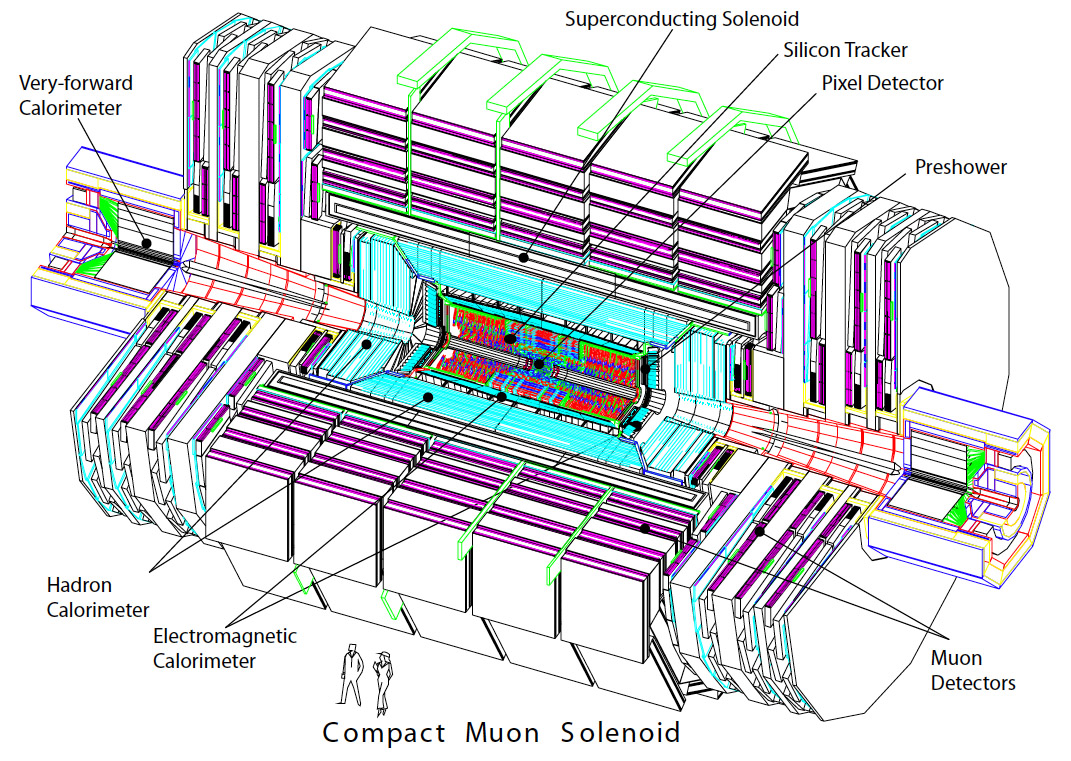
\includegraphics[width=0.75\textwidth]{plots/CMS/cms.png}
\caption{A 3-d cut-away view of the CMS detector, showing the relative position and size of the subdetectors as well as the orientation of the experiment with repsect to the beamline.}
\label{fig:cms:cms_full} 
\end{figure}

\begin{figure}[htb]
\centering
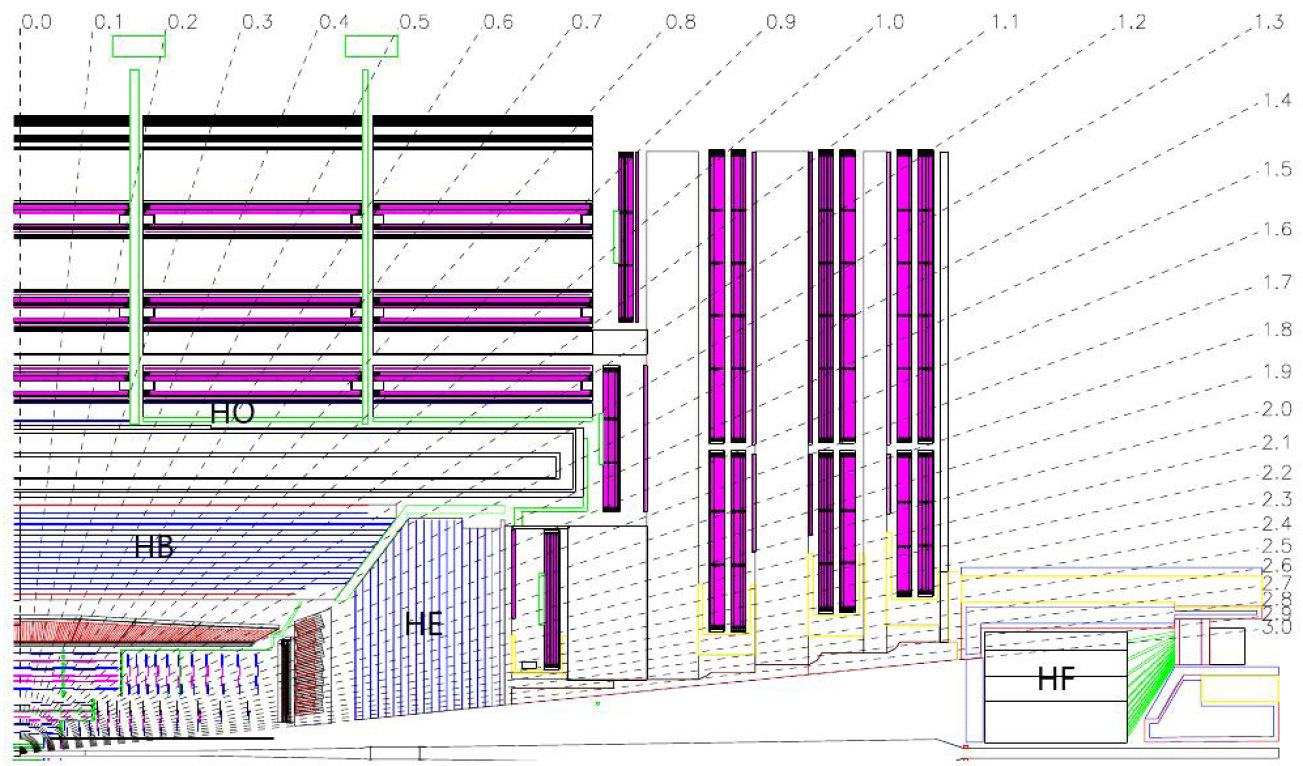
\includegraphics[width=0.75\textwidth]{plots/CMS/cms_quarter.png}
\caption{Quarter-view schematic of the CMS detector showing the arrangement of the subsystems. Radially arranged dotted lines indicate the pseudorapidity ($\eta$) coverage.}
\label{fig:cms:cms_quarter}
\end{figure}

% %% finish section and uncomment
% \subsection{Coordinates \& Units}
% Before describing the detector, an overview of standard terminology for the coordinate system, units, and other commonly used terminology is provided.
% \begin{itemize}
%     \item  rapidity
%     \item $\Delta R = \sqrt{\Delta\eta^2+\Delta\phi^2}$
% \end{itemize}
% % 



\subsection{Magnet}\label{ch:cms:magnet}
The namesake superconducting magnet provides a uniform $|\vec{B}| = 3.8 \,\mathrm{T}$ field at inner radii and a field of $|\vec{B}| = 2 \,\mathrm{T}$ at radii outside of the magnet. This is achieved using a liquid helium-cooled niobium-titanium superconductor mechanically supported by a high-purity aluminum chassis. The operational temperature of the magnet is $T = 4.6 \,\mathrm{K}$, which maintains the current and temperature below the critical values so that $|\vec{B}| = 3.8 \,\mathrm{T}$ field~\cite{Acquistapace:1997fm}.

\begin{figure}[htb]
\centering
  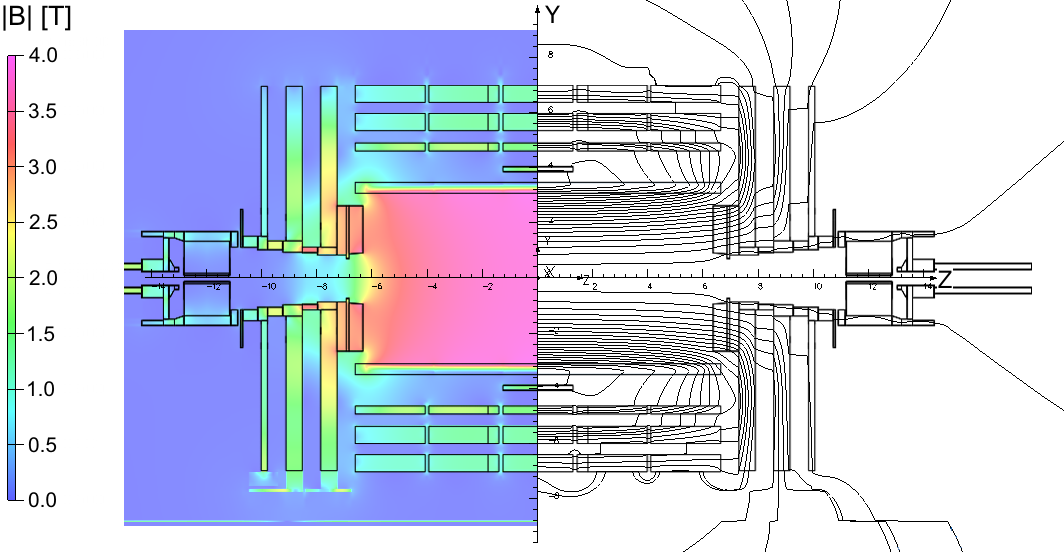
\includegraphics[width=0.9\linewidth]{plots/CMS/magnetic_field.png}
  \caption{Diagram depicting the magnetic field strength and field lines from the CMS superconducting solenoid~\cite{Chatrchyan:2009si}.}
  \label{fig:cms:bfield}
\end{figure}
With an inner radius of 6 meters, the solenoid bore houses the silicon tracker, electromagnetic calorimeter, and the hadronic calorimeter. The solenoid ensures a uniform inner magnetic field of $|\vec{B}| = 3.8 \,\mathrm{T}$ along the $z$-axis for these sub-systems. On the outer radius of the solenoid, muon chambers are interspersed with the steel return yoke. The role of the return yoke is two-fold---extend uniformity and strength of the magnetic field outside of the solenoid and to act as an absorber layer for the muon chambers. 

%%%%%%%%%%%%%%%%%%%%%%%%%%%%%%%%%%%%%%%%%%%%%%%%%%%%%
%                   Tracker 
%%%%%%%%%%%%%%%%%%%%%%%%%%%%%%%%%%%%%%%%%%%%%%%%%%%%%
\subsection{Trackers}\label{ch:cms:tracker}
%% intro and purpose
The innermost detector system is the silicon tracker. The tracker measures the trajectory of charged particles from the collision point, and is designed to provide efficient and high-precision position reconstruction of charged particle trajectories through the tracker volume. In addition to providing high-resolution momentum information, the tracker should be able to identify isolated electromagnetic clusters, as in the $W\rightarrow e\nu$ and $Z \rightarrow ee$ channels, and to separate them from non-isolated electrons\cite{Karimaki:368412}.

%% design considerations
Other design considerations are the proximity of the inner tracker to the collision point and the material budget. Due to its close proximity to the beamline, the tracker is subjected to a high particle flux, with thousands of particles per bunch crossing every $25\,\mathrm{ns}$. This necessitates a radiation-hard detector with fast readout and high granularity to reduce multiple-occupancy per channel. However, the amount of material in the detector---including the supporting electronics, cabling, and cooling systems---increases the amount of bremsstrahlung, which degrades the resolution of isolated electron measurements. Therefore the amount of detector material also needs to be minimized.

Given these design and operational considerations, the tracker uses silicon technology in the form of pixel and strip detectors. The silicon pixels are a p-n junction operated under a reverse-bias voltage. Charged particles traversing the depletion zone create electron-hole pairs, which drift under the reverse-bias and are collected by readout electronics.

%% design/construction
%% Pixel detector
The inner tracking system is composed of a silicon pixel detector, with 3 layers of pixels in the barrel ($r=4.4 \,\mathrm{cm}$, $7.3 \,\mathrm{cm}$, and $10.2 \,\mathrm{cm}$, $\mathrm{length}=53\,\mathrm{cm}$) and 2 layers of pixels in the end-cap region (inner radius of 6 cm, outer radius 15 cm, located at $|z|=34.5 \,\mathrm{cm}$ and $|z|= 46.5 \,\mathrm{cm}$). The individual pixels are 150x100$\mu\mathrm{m}$, with 60 million pixels, where the fine segmentation is intended to minimize track occupancy per channel. A schematic depicting the geometry of the inner and outer tracking systems is shown in Figure~\ref{fig:cms:tracker}

%Strip Detector

Surrounding the inner tracker, the outer tracker is a series of silicon strip detectors. The tracker inner barrel (TIB) covers $20 \,\mathrm{cm} < r < 55 \,\mathrm{cm}$, and an additional six-layer outer barrel (TOB) extending to $r<116cm$.  The TIB spans $\pm$ 80 cm and TOB spans $\pm$ 118 cm in $z$. 
Tracker disk segments with strips arranged in rings are located within the inner radius of the TOB at $z$ position just outside of the TIB. Further nine endcap ring layers are positioned beyond the $z$ extent of the TOB, between $z=\pm$95.2cm and $\pm$ 264cm. Depending on the position, each layer contains between 2 and 7 rings of detector with inner radius 21.8cm-39cm and outer radius 60.8cm.

\begin{figure}[htb]
\centering
  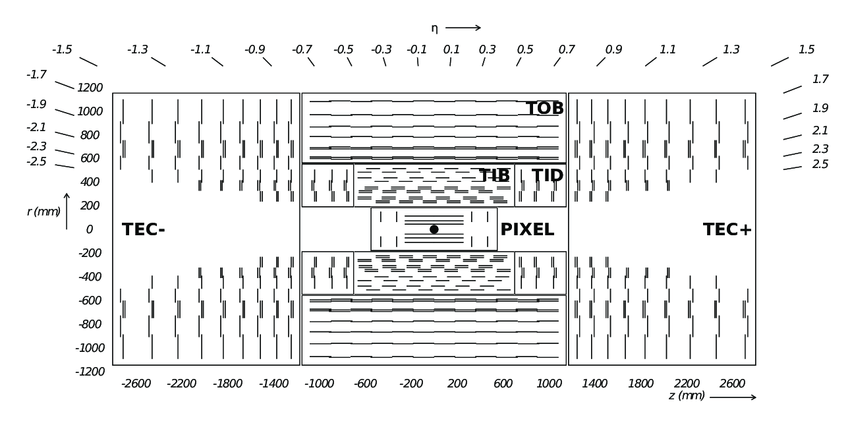
\includegraphics[width=0.7\linewidth]{plots/CMS/r-z-slice-of-the-CMS-Tracker.png}
  %https://cds.cern.ch/record/40524
  \caption{Schematic of the CMS tracking system. The silicon pixel detector is surrounded by the inner (TIB) and outer (TOB) barrel strip detectors. The endcap (TEC) strip detectors provide forward coverage up to |$\eta$|<2.5.~ \protect\cite{CMS_tracker_diagram}}
  \label{fig:cms:tracker}
\end{figure}


%%%%%%%%%%%%%%%%%%%%%%%%%%%%%%%%%%%%%%%%%%%%%%%%%%%%%
%                   ECAL 
%%%%%%%%%%%%%%%%%%%%%%%%%%%%%%%%%%%%%%%%%%%%%%%%%%%%%
\subsection{Electromagnetic Calorimetry}\label{ch:cms:ecal}
 % Cite CMS ECAL TDR
%% intro/purpose
The energy carried by electrons and photons is measured by the electromagnetic calorimeter (ECAL). The ECAL is a homogenous and hermetic calorimeter situated just outside of the silicon tracker, which measures the energy carried by electrons and photons.
%% Design  considerations
Driving factors determining the design of the ECAL is the need for a fast response time sufficient for collisions occuring every 25ns as well as a high-resolution measurement necessary for the $H\rightarrow \gamma \gamma$ measurement. To this end, the active material is a scintillating lead tungstate ($\mathrm{PbWO_4}$) crystal. Incident electrons and photons create an electromagnetic shower within the crystal. As the shower propagates, scintillation light is produced by excitations in the crystal lattice caused by the particles in the shower. The scintillation light, proportional to the energy deposited by the incident particle, is collected and read out by a photodiode\cite{CERN-LHCC-97-033}.

\begin{figure}[htb]
\centering
  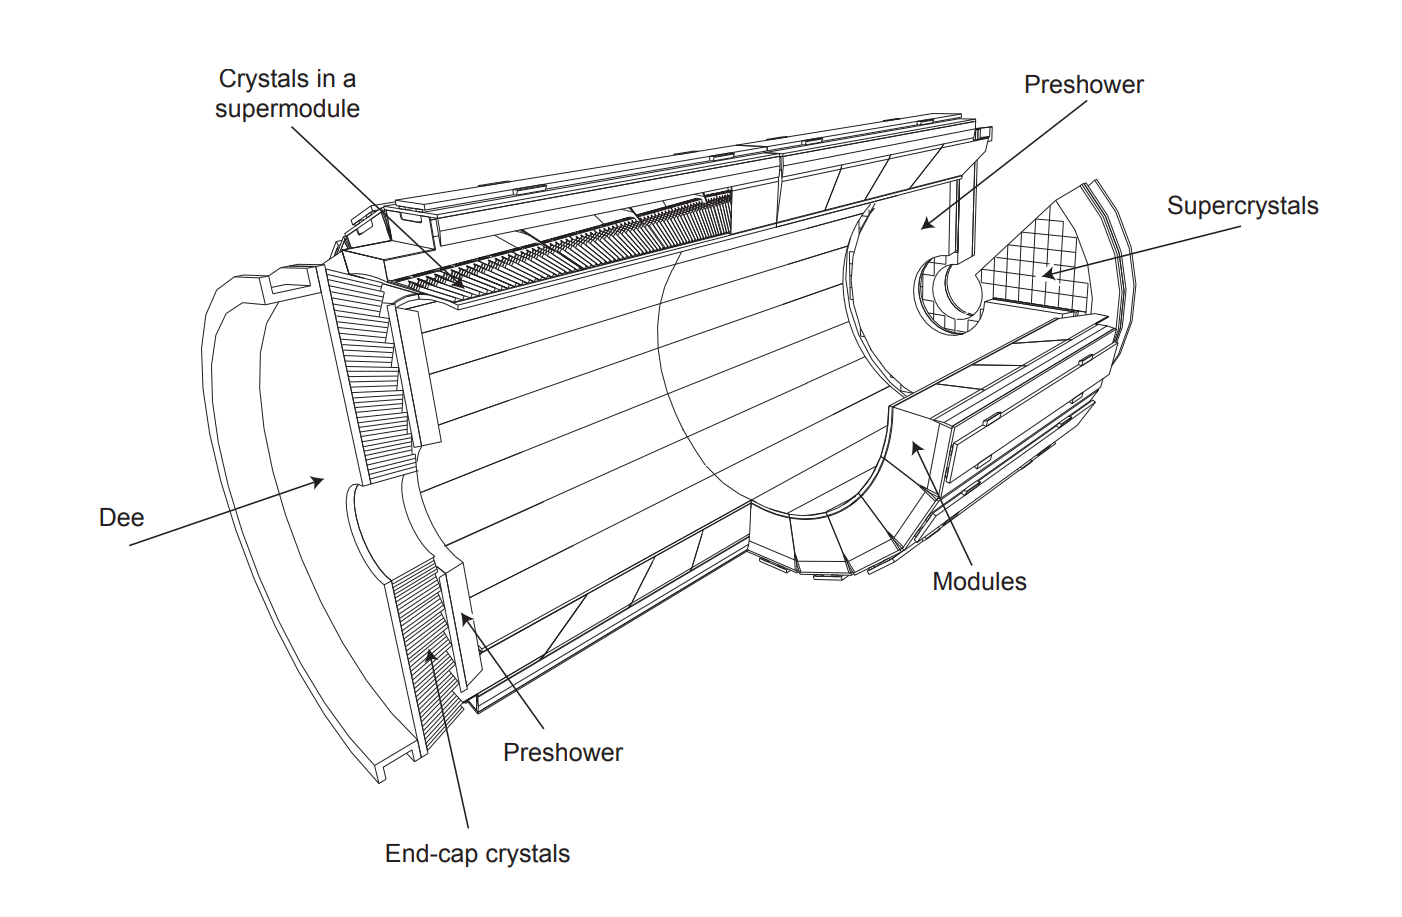
\includegraphics[width=0.9\linewidth]{plots/CMS/ecal_1.PNG}
  %https://cds.cern.ch/record/40524
  \caption{Schematic of the ECAL demonstrating the location and orientation of the crystals in the barrel and endcap. The radial pointing of the crystals is visible.~\protect\cite{Benaglia_2014}}
  \label{fig:cms:ecal1}
\end{figure}

\begin{figure}[htb]
\centering
  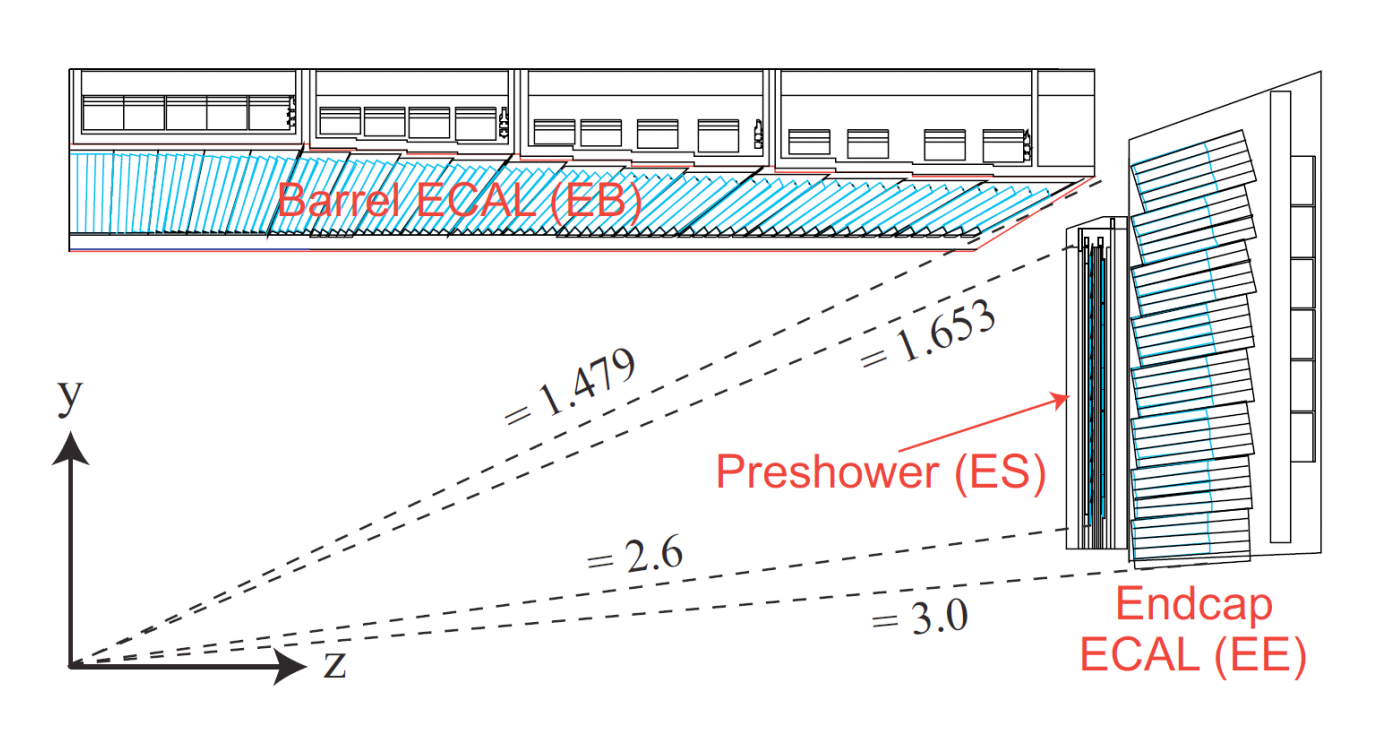
\includegraphics[width=0.7\linewidth]{plots/CMS/ecal_2.PNG}
  %https://cds.cern.ch/record/40524
  \caption{Quarter-view of the ECAL showing the position and orientation of the crystals.~\protect\cite{Benaglia_2014}}
  \label{fig:cms:ecal2}
\end{figure}

In the barrel region, the wedge-shaped crystals (approximately 2.2x2.2x23cm, corresponding to 26 radiation lengths in depth) are arranged radially, covering up to $|\eta|<1.49$. The endcap provides coverage from $1.47<|\eta|<3.0$, with the 3x3x22cm (approximately 25 radiation lengths)  crystals arranged approximately parallel to the beamline. Crystal dimensions are compatible with electromagnetic shower sizes in $\mathrm{PbWO_4}$. The orientation of the crystals depends on their $|\eta|$ position, as they are angled towards $3\deg$ of the collision point, as shown in Figure~\ref{fig:cms:ecal2}.
%% Radiation Damage
 The $\mathrm{PbWO_4}$ crystals are radiation hard, but exposure to radiation damages the crystals, producing color centers which reduce the transparency of the crystal volume. Transparency loss and the associated change in energy response is most prominent in regions of high $|\eta|$ which were subjected to the highest levels of radiation\cite{Cipriani:2018ule}. These defects can anneal during times without collisions. The ECAL is equipped with a laser system which monitors the transparency of the crystals. Calorimeter performance can be maintained by accounting for the transparency loss experienced by indivdiual crystals\cite{CERN-LHCC-97-033}.   

%% capabilities
The ECAL energy resolution is described in Equation~\ref{eq:cms:ecalresolution}. 
\begin{equation}
\frac{\sigma(E)}{E}=\frac{2.8\%}{\sqrt{E}} \oplus \frac{120 MeV}{E} \oplus 0.3\%
\label{eq:cms:ecalresolution}
\end{equation}
The contributions to the energy resolution are, respectively, the stochastic term, electronics noise term, and the constant term. Stochastic term, $2.8\%/\sqrt{E}$, accounts for statistical fluctuations in shower detection, and it is small due to ECAL being a homogenous calorimeter. The constant noise term, $0.3\%$, includes detector calibration and instability\cite{Adzic:2007mi}.
%%%%%%%%%%%%%%%%%%%%%%%%%%%%%%%%%%%%%%%%%%%%%%%%%%%%%
%                   HCAL 
%%%%%%%%%%%%%%%%%%%%%%%%%%%%%%%%%%%%%%%%%%%%%%%%%%%%%
\subsection{Hadronic Calorimeter}\label{ch:cms:hcal}
%% intro/purpose
The Hadronic Calorimeter (HCAL) measures the energy of charged hadrons. 
%% purpose
%% design consideration
%% design/construction

The HCAL has four subsystems---Barrel (HB), Endcap (HE), Outer (HO), and Forward (HF)---with a quarter slice of the detector shown in Figure~\ref{fig:cms:hcal}.  HB, HE, and HO are sampling calorimeters using plastic scintillator and steel and brass absorbers. HB extends from the outside of the ECAL to the inner radius of the solenoid coil: $r=1.77\,\mathrm{m}$ - $r=2.95\,\mathrm{m}$ and covers $|\eta| < 1.3$ with an $\eta-\phi$ segmentation of $0.87\times0.87$. The interior absorber is a $40\,\mathrm{mm}$ thick steel plate, followed by eight layers of $50.5\,\mathrm{mm}$ thick brass plates interleaved with $3.7\,\mathrm{mm}$ thick plastic scintillator tiles, and final steel plate absorber 75mm thick, providing a total interaction length of $5.8\,\lambda_I$. The layers of HO are situated at the outer radius of the solenoid, designed to catch showers for high energy hadrons that are not contained within the other HCAL subsystems. There is an extra HO layer near $|\eta|\approx 0$ where the interaction depth of the HB is shortest. The construction of HB and HE are cylindrically nested alternating layers of brass absorber and scintillator, with the first absorber layer made of steel. The HE extends coverage to $|\eta| < 3$, and consists of 10 layers of alternating scintillator and brass absorber, with a steel first absorber layer.

HF is a sampling calorimeter using quartz fibers embedded in steel. It is situated in the far forward region of the detector, with coverage up to $|\eta| < 5.2$. Due to its position, the HF experiences significantly higher particle flux than the other HCAL subsystems and the HF needed to have extremely fast response and radiation hardness
\cite{CERN-LHCC-97-031}.

\begin{figure}[htb]
\centering
  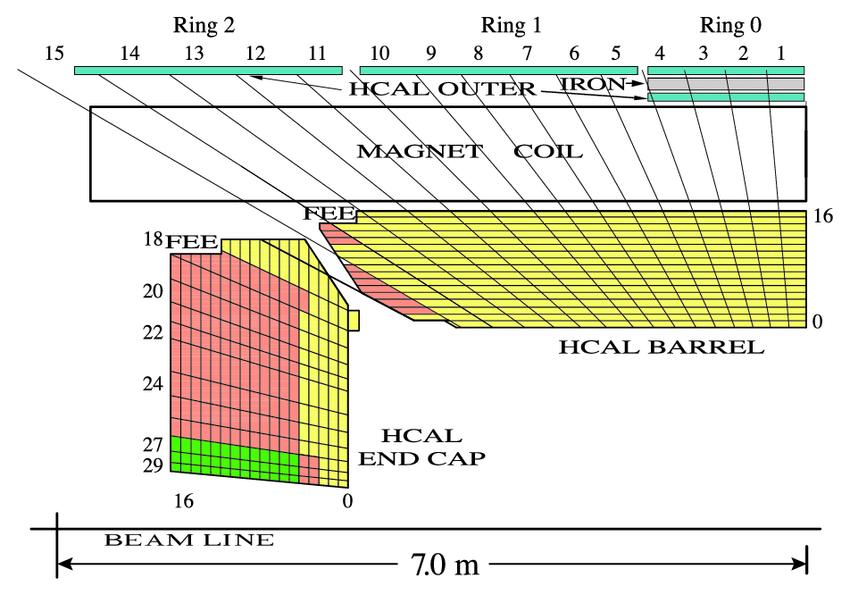
\includegraphics[width=0.7\linewidth]{plots/CMS/HCAL-quarter.png}
  %https://cds.cern.ch/record/40524
  \caption{Quarter-view of the HCAL showing the positioning and segmentation of the barrel, endcap, and outer subsystems.~\protect\cite{Chatrchyan:1223869}}
  \label{fig:cms:hcal}
\end{figure}


The HCAL is a sampling calorimeter. Incident charged hadrons undergo multiple scattering within the absorber material, producing hadronic showers that propagate in the direction of the particles intial trajectory. As the showers develop, they pass through the absorber layer and traverse the scintillator layer, where the particles in the shower induce excitations resulting in scintillation light. The light is wavelength shifted and carried by optical fibers to a photodiode where it is read out and digitized. In the HF, quartz fibers produce Cherenkov light. 



%% capabilities
The energy resolution of the HCAL, described in Equation~\ref{eq:cms:hcal_res} is representative of a sampling calorimeter. Resolution is affected by the limited detector volume available to the HCAL\cite{Cavallari_2011}.

\begin{equation}
\frac{\sigma(E)}{E}=\frac{110\%}{\sqrt{E}} \oplus 7.3\%
\label{eq:cms:hcal_res}
\end{equation}
The stochastic term (${110\%}/\sqrt{E}$) accounts for the statistical fluctuations in shower detection, which is relatively large for the HCAL due to its design as a non-compensating sampling calorimeter. The constant $7.3\%$ term is due to detector calibration limitations.

\subsubsection{HCAL Reconstruction Algorithms}
In HB and HE, the total pulse width from light collection and electronic readout is larger than the 25\ns separation between LHC bunch crossings. Output from the HPD is digitized and integrated in 25\ns-wide bins. Approximately 60\% of the pulse width is contained within the first 25\ns and and 90\% of the pulse is contained within the first 50\ns. LHC Run II conditions with 25\ns separation between bunch crossings potentially produces readout with substantial overlap between pulses generated by interactions from consecutive bunch crossings. An algorithm to perform hit reconstruction in each calorimeter tower was developed for Run II in order to mitigate the effect of out-of-time pileup events on the energy resolution of the HB and HE readout channels. This was achieved by assuming the presence of out-of-time pileup interactions from the immediately precedent and antecedent bunch crossings. A fitting template is constructed out of 3 HCAL pulse shape templates, where the free parameters are the arrival times and normalizations of each pulse as well as a floating baseline to accommodate noise. The resulting normalization of the in-time pulse determines the energy for the reconstructed hit in each channel. 
%% do i have a diagram demonstrating the fits
In addition to providing the offline HCAL hit reconstruction, the algorithm is used in HCAL operations and data validation. In addition to hit energy, the fitting procedure determines the arrival time with a resolution of 1\ns. This provides the ability to monitor and calibrate the relative timing of the channels in HB and HE. 
%%%%%%%%%%%%%%%%%%%%%%%%%%%%%%%%%%%%%%%%%%%%%%%%%%%%%
%                   Muon 
%%%%%%%%%%%%%%%%%%%%%%%%%%%%%%%%%%%%%%%%%%%%%%%%%%%%%
\subsection{Muon System}\label{ch:cms:muons}
%% intro/purpose
The outermost detector system is the muon chambers. Situated around the return yoke, the muon detectors are used for muon triggering, muon identification, and muon momentum measurement. Particles that make it through CMS and reach the muon systems are almost exclusively muons. Muon detector information is combined with tracking information to enhance muon reconstruction.
The muon system uses three detector technologies: resistive plate chambers (RPC), drift tubes (DT), and cathode strip chambers (CSC)\cite{CMS:1997iti}. 
% blahhhh

The barrel region technology is drift tubes, with coverage up to $|\eta| < 1.2$. These are suitable due to the fairly uniform magnetic field and low particle flux. The barrel region is constructed of four cylindrically nested sets of rectangular drift tube components, with 12 segments in $\phi$, and panels at each radius grouped to form a muon station. The stations are located in alternating layers with the magnetic field return yoke. Each station consists of 8 layers of drift tubes. The arrangement of the barrel muon stations can be seen in Figure~\ref{fig:cms:muons}. The drift chambers containing a $\mathrm{CO_2}$/Argon gas mixture, which has a drift velocity of 55 $\mu$m/ns (about 400ns maximum drift time) \cite{Chatrchyan:2013sba}.
\begin{figure}[htb]
\centering
  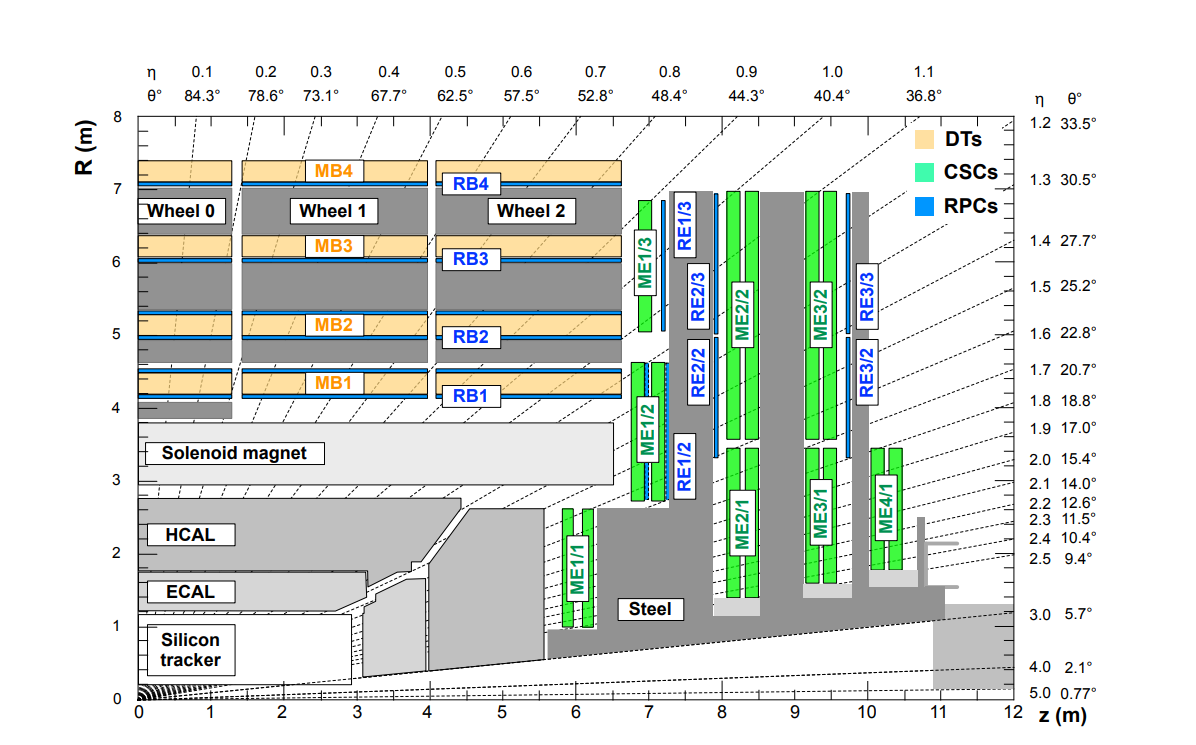
\includegraphics[width=0.7\linewidth]{plots/CMS/cmsmuon.png}
  \caption{Quarter-view of the CMS muon system illustrating the position of the DT, CSC, and RPC detectors within the magnetic field return apparatus \protect\cite{Chatrchyan:2013sba}.}
  \label{fig:cms:muons}
\end{figure}


%% design/construction
The endcap muon detectors use a cathode strip chamber (CSC). CSC are multi-wire proportional chambers with a cathode strip as the readout and can provide a precise location of ionization. The endcap stations are grouped by $z$ position, covering $1.2 < |\eta| < 2.4$. CSCs are used in the endcap regions because their high granularity and short drift distance makes them more suitable for the higher event rate and non-uniform magnetic field in this region. The CSC strips are arranged radially, and contain 6 layers which each provide a 2-coordinate hit position in the $r-\phi$ plane. Additional readout is taken from the anode wires, which provide a rough position meaurement in $r$.
%% RPC trigger
In addition to the CSC and DT which provide full $\eta$ coverage up to $|\eta| < 2.4$, the muon system also utilizes a set of resistive plate chambers as an independent trigger system. The RPCs cover $|\eta| < 1.6$, and are a double-gap system operated in avalanche mode. The RPCs have poor position resolution, but have a response time of 1 ns and can be used to measure correct bunch crossing time at the highest LHC luminosities. 

\section{Data Acquisition and Trigger}
The LHC provides pp collisions with a bunch spacing of 25\ns, which corresponds to a rate of 40 MHz. With multiple collisions occurring per bunch crossing, the event rate incident upon CMS is much higher than 40 MHz. The maximum final event rate needs to average on the order of 1 kHz, limited by the storage and data acquisition. In order to reduce the event rate while maintaining a high efficiency of selecting interesting physics processes, CMS uses a trigger system to make quick calculations and decisions about which events to keep or discard. 

\subsection{Trigger}
The trigger systems are a two-stage decision-making tool, which reduce the event rate based on trigger primitives at varying levels of complexity. The stages of the trigger system are the Level One (L1) trigger and the and the High-Level Trigger (HLT)\cite{Khachatryan:2016bia}. 

The L1 trigger resides on custom boards with field-programmable gate arrays (FPGAs). These contain pattern recognition algorithms that are able perform rough calculations to create candidate tracks and calorimeter clusters used for classification. The L1 operates with a latency of 3.8 $\mathrm{\mu s}$ per event, and full detector readout is held in a buffer while the L1 decision is made. L1 objects are energy clusters from ECAL and HCAL and muon track segments. Decisions are based on rough reconstrution of objects such as electrons, photons, muons, jets, and \met.  Information flow in the L1 trigger is shown in Figure~\ref{fig:l1_trigger}. The output rate of the L1 is limited to 100 kHz. Events which pass the L1 trigger are used to seed the more robust HLT analysis\cite{Khachatryan:2016bia}. 

\begin{figure}[htb]
\centering
  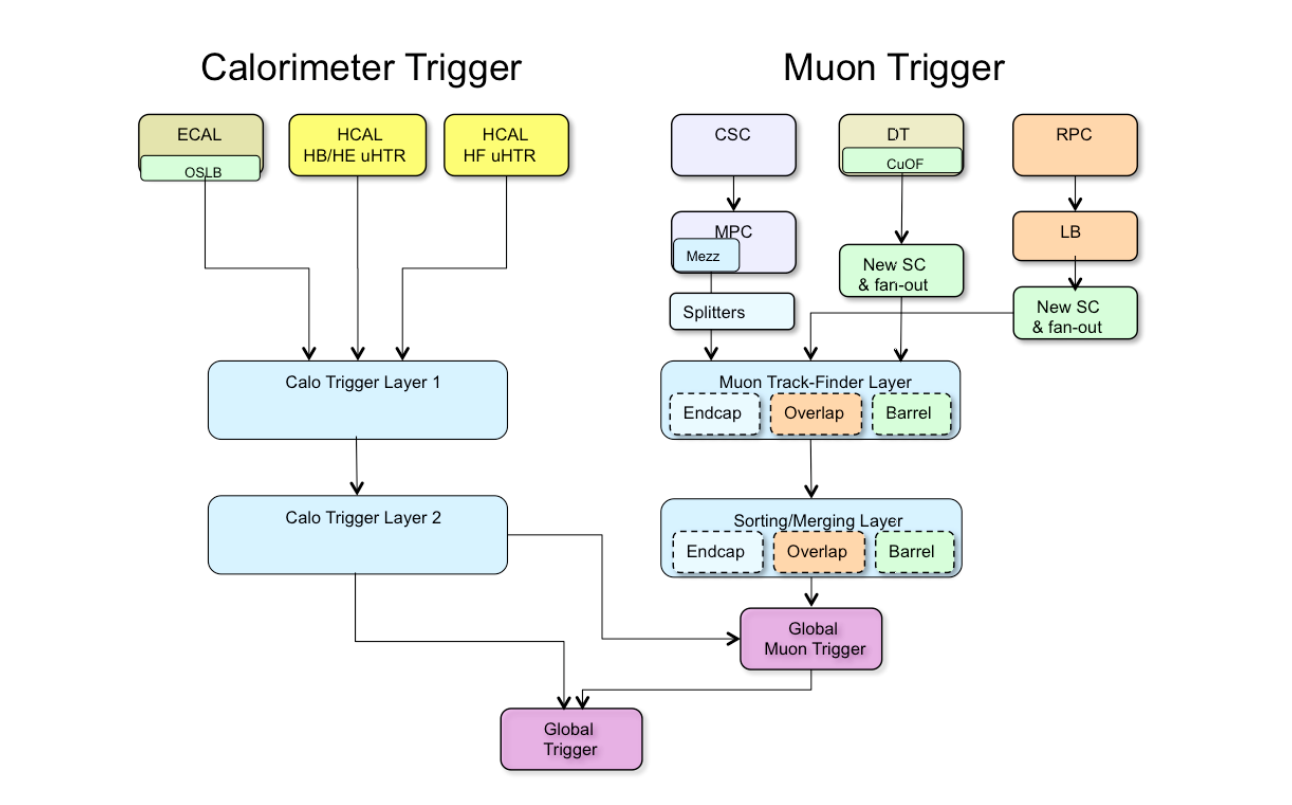
\includegraphics[width=0.75\linewidth]{plots/CMS/l1.PNG} 
  %https://cds.cern.ch/record/40524
  \caption{Schematic workflow of the L1 trigger. Information is first processed by the calorimeter and muon triggers, then combined at a global trigger \protect\cite{Cadamuro:2017slr}.}
  \label{fig:l1_trigger}
\end{figure}

The HLT system is a processor farm containing $O(10,000)$ CPU cores \cite{Adam:2005zf}. Here, fragments of events are combined to form complete events. The algorithms used to perform event reconstruction at the HLT level produce a similar quality as those used in the offline reconstruction, and the HLT has access to the full event readout. HLT reconstruction is seeded by the L1 trigger decision. HLT paths allow for quick reconstruction by selectively filtering events as the reconstruction steps proceed---decisions are based on easily reconstructable calorimeter clusters or muon tracks, while computationally expensive track finding is only performed on events which pass the other criteria. Events passing selection by the HLT are saved to be fully reconstructed and stored for analysis use. The average event selection rate by the HLT is 1000 Hz \cite{Khachatryan:2016bia}. 

\subsection{Data Storage and Processing}
Those events which pass the HLT filtering are stored on disk and eventually transferred to a Tier-0 computing center for full offline reconstruction and permanent storage. Data is stored and processed in part of a global computing grid, with multiple copies of datasets stored at computing centers around the world. 
%%%%%%%%%%%%%%%%%%%%%%%%%%%%%%%%%%%%%%%%%%%%%%%%%%%%%
%%%%%%%%%%%%%%%%%%%%%%%%%%%%%%%%%%%%%%%%%%%%%%%%%%%%%
\section{Detector Simulation}
Physical processes originating at the pp collision point are simulated by a series of event generators, which are described in a later chapter. In addition to generating the pp collision products, the simulated event sets must also incorporate effects due to the full chain of particle interactions and detector readout in CMS.

Particle propagation through the detector volume is modeled by GEANT4\cite{AGOSTINELLI2003250}. This toolkit allows a full geometric reconstruction of the detector, and handles the particle transport through the materials. Particle decays, bremsstrahlung, electromagnetic interactions, and hadronic interactions with the materials are modeled, as well as the effect of the magnetic field \cite{ALLISON2016186}. GEANT4 also handles detector response simulation, i.e. the simulation of optical photon production in a scintillator. Readout electronics, including associated noise, are also simulated.

Following the simulation of detector readout electrons, the simulated information is in the same format as data collected by the detector. At this stage, the full CMS reconstruction is applied to the simulation in the same way it is applied to data. 
%%%%%%%%%%%%%%%%%%%%%%%%%%%%%%%%%%%%%%%%%%%%%%%%%%%%%
%%%%%%%%%%%%%%%%%%%%%%%%%%%%%%%%%%%%%%%%%%%%%%%%%%%%%

\section{Luminosity Calibration}\label{ch:cms:lumi}
An accurate luminosity measurement is necessary to provide an estimate of the correct production yield for the W and Z bosons. Luminosity calibration at CMS is calculated by readout from dedicated luminosity monitors, rates of reconstructed objects in CMS, and dedicated LHC configurations to perform Van der Meer scans.

During LHC operation, measurement of \phil{the} instantaneous luminosity is based on the event rate recorded by several detectors. Online luminosity information is provided by dedicated luminometers---the Pixel Luminosity Telescope (PLT), Fast Beam Conditions Monitor, and the HCAL Forward calorimeter (HF)---which are operated on a separate readout from CMS physics data. Offline luminosity monitoring is based on data collected by CMS: rates of reconstructed pixel cluster counts and rates of tracks in the muon drift tubes\cite{Lujan:2647819}.

Absolute calibration is determined by a Van der Meer (VdM) scan \cite{vanderMeer:1968zz}\cite{Balagura:2011yw}, which utilizes a dedicated LHC configuration to scan the opposing proton beams transversely across each other. Data collected by CMS during these scans is used to reconstruct a beam profile and to determine the relationship of the instantaneous luminosity to the rates measured by the various luminosity monitoring systems.

Uncertainties in the luminosity measurement come from two primary categories. Normalization uncertainties, treated as uncorrelated, come from uncertainties of length scales and correlations when performing VdM scans. Integration uncertainties are related to detector operation and nonlinear detector response corrections\cite{CMS:2018elu}.
\chapter{Event Reconstruction}\label{ch:reco}
Particles from collisions pass through CMS, producing signals in the various subdetectors. Events are reconstructed from the information delivered by the subsystems. This section outlines the method for reconstructing and identifying various components of events.

%%%%%%%%%%%%%%%%%%%%%%%%%%%%%%%%%%%%
%%      Track
%%%%%%%%%%%%%%%%%%%%%%%%%%%%%%%%%%%%
\section{Tracks}
Track reconstruction combines hits in the pixel and strip detectors, which are fit to construct tracks. Zero-suppressed signals in the pixel and strip detectors are clustered into hits, which provides hit position and uncertainty information. The track finding algorithm is an interative process which uses an implementation of the combinatorial Kalman Filter. The combinatorial Kalman Filter provides a combintation of pattern recognition and track fitting. The 6-pass iterative procedure initially finds the tracks that are easiest to identify, removes the hits associated with these tracks, and reiterates over the remaining collection of tracker hits. \cite{Chatrchyan:2014fea}

\phil{I think you mean Electron Tracks} Tracks are seeded using three hits in the inner pixel detector which correspond approximately to a track from the beam spot. The innermost tracker layers are used because electrons undergo significant energy and trajectory loss due to bremsstrahlung and many charged pions undergo inelastic collisions as they traverse the inner tracking layers. The highly granular pixel detector has lower occupancy than the outer strip detectors. These seed hits combined with the beam spot location provide enough information to derive parameters describing a helical trajectory as the particle moves through the magnetic field. The tracks are propagated outwards to subsequent tracker layers, incorporating additional hits if a $\chi^2$ is below a target threshold. Kalman filtering is then used to update the parameters of the track \cite{Adam:2005cg}. \phil{Not sure if you are talking about just electron reco or all, I would claify and if its electrons add the words Gaussian Sum Filtering(GSF) }

Effects of tracker and support material on the energy loss and trajectory of particles traversing the tracker are also accounted for in this process. These effects are incorporated by Runge-Kutta based iterative propagator to describe a parametrized material distribution of the CMS detector and relevant interactions assuming every track is a pion. 

Spurious track segments not corresponding to actual particle trajectories are removed after reconstruction. Requirements on minimum fit quality ($\chi^2/NDF$), proximity to the primary vertex ($\Delta z$), and proximity to the beam spot ($d_0/\delta d_0$) are used to remove such tracks. 

%%%%%%%%%%%%%%%%%%%%%%%%%%%%%%%%%%%%
%%      PV
%%%%%%%%%%%%%%%%%%%%%%%%%%%%%%%%%%%%
\section{Primary Vertex}
Primary vertex (PV) reconstruction ensures the position of each proton-proton interaction in every event. Reconstructed tracks with high fit quality and several tracker hits are propagated back to the beamline. A clustering algorithm combines the position of closest-approach to the beamline into vertices based on their $z$-axis location \cite{Chatrchyan:2014fea}. The clustering algorithm currently used is a deterministic annealing algorithm, which produces a high performance in successful cluster finding in a noisy environment \cite{Chabanat:2005zz}

%%%%%%%%%%%%%%%%%%%%%%%%%%%%%%%%%%%%
%%      electrons
%%%%%%%%%%%%%%%%%%%%%%%%%%%%%%%%%%%%

\section{Electron Reconstruction}\label{ch:reco:ele}
% \subsection{Electron Reconstruction}
Electron reconstruction starts with an energy deposition in the ECAL, known as a supercluster. With the supercluster as a seed, a track is projected inwards from the ECAL, and pairs of hits in the silicon pixel tracker are searched for. From these, further tracker hits compatible with the trajectory are incorporated into the electron reconstruction. Due to Bremsstrahlung, electrons lose significant amounts of energy and change trajectory. The Bremsstrahlung losses are accounted for using a set of possible energy loss models. This is incorporated using a weighted technique known as a Gaussian Sum Filter (GSF) algorithm. 

From the electron track reconstruction, multiple observables describing the kinematics of the electron, the surrounding event, and quality of the reconstruction are produced. These are later used to identify candidate electrons originating in the signal processes for this analysis,as described in Chapter~\ref{ch:IdIso:Ele}.  

%%%%%%%%%%%%%%%%%%%%%%%%%%%%%%%%%%%%
%%      muons
%%%%%%%%%%%%%%%%%%%%%%%%%%%%%%%%%%%%
\section{Muon Reconstruction}\label{ch:reco:muon}

% \subsection{Muon Reconstruction}\label{ch:reco:mu:type}
\subsubsection{Standalone Muons}
A standalone muon track is built solely from information collected by the muon chambers. Energy depositions in the CSC and DT are combined as track segments. These are used as seeds for track reconstruction from the muon chambers CSC, DT, and RPCs, which are combined using a Kalman filter\cite{Sirunyan:2018fpa}. 

\subsubsection{Global Muons}
%% Our ID requires a global muon
The global muon reconstruction starts with an energy deposition in the muon chambers which is propagated inwards towards the inner tracker. Standalone muon tracks are used as the seed for global muon reconstruction. Kalman filter techniques are used to combine the tracker and muon track segments to form a global muon. Energy loss effects due to detector material and support structure between the tracker and muon chambers are also accounted for. Global muon reconstruction improves momentum resolution for muons with $\pt > 200 \GeV$.

\subsubsection{Tracker Muons}
Tracker muons are muons which are identified as tracks in the tracker with at least $\pt > 0.5$ and $p > 2.5\GeV$. Tracker muon reconstruction is similar to global muon reconstruction, but the seed is a track segment from the inner tracker as opposed to a muon track segment.


\phil{Given you define PF Iso before particle flow, I would just move the particle flow section up}

%%%%%%%%%%%%%%%%%%%%%%%%%%%%%%%%%%%%
%%      Particle Flow
%%%%%%%%%%%%%%%%%%%%%%%%%%%%%%%%%%%%
\section{Particle Flow}
The CMS detector is suited to using the particle flow (PF) technique in event reconstruction. The general principal of PF is to combine information from tracks and calorimeter deposits into one object. This analysis relies on the transverse missing energy (\met) as provided by the particle flow algorithm. This section describes the PF algorithm as well as the PF \met. 

\subsection{Particle Flow Reconstruction}
\subsubsection{Basic Elements}
The basic elements of the PF algorithm are tracks in the tracker, track segments in the muon chambers, and energy clusters from the ECAL and HCAL. 
Calorimeter clustering begins with a local maximum energy deposition as a seed, and are grown by incorporating neighboring cells with an energy above a certain threshold. The threshold is 2$\sigma$ above the standard electronic noise of the subdetector (80 MeV in ECAL Barrel, 300 MeV in ECAL Endcap, and 800 MeV in the HCAL). 
An individual particle will produce multiple PF elements, and a linking algorithm is used to incorporate the elements from each subsystem into one object. 

\subsubsection{Linking Algorithm}
The linking algorithm finds the PF elements from each detector that correspond to individual objects and groups them together. Tracks are associated with calorimeter clusters by extrapolating from the outermost tracker hit, through the preshower and ECAL, and one interaction length into the HCAL. Pairwise matching between the extrapolated track and nearby calorimeter clusters is performed, and linking occurs if the track extrapolation falls within the cluster cells as measured in the $(\eta,\phi)$ plane for the ECAL barrel and HCAL and $(x,y)$ plane for the ECAL endcap and preshower. Calorimeter-to-calorimeter cluster linking is performed in a similar way by extrapolating clusters between the ECAL and HCAL, seeded with the cluster from the more granular detector. 

In cases where multiple objects from one detector are linked with the same object from another detector, only the pair with the closest link (best fit) is kept. 

Bremsstrahlung photons in the ECAL are linked by searching for ECAL clusters which are consistent with a tangential projection from the GSF electron track reconstruction. Additionally, bremsstrahlung photons radiated within the tracker are identified by tracks corresponding to photon conversion and can be linked to the GSF electron. 

Linking information from the muon chambers is also performed, and is described in the muon reconstruction Section~\ref{ch:reco:muon}.


\subsection{\met}
Missing transverse energy (\met) is defined as the negative vector sum of all transverse momenta in an event, as in Equation~\ref{eq:met}.
\begin{equation}
    E_T^{miss}=-\sum_{p} \vec{p_T}
    \label{eq:met}
\end{equation}
Particle flow \met is constructed from reconstructed PF particles.

\chapter{Data Samples and Event Selection}\label{ch:data}
The data used in this analysis were collected in late 2017 by the CMS Experiment during Run II of the LHC. At this time, the LHC delivered two sets of \pp collisions, at \serag (2017G) and at \serah (2017H). This chapter details the information related to data collection and Monte Carlo simulations associated with these data taking periods. Details regarding the object identification criteria and event selection are also provided.

%%%%%%%%%%%%%%%%%%%%%%%%%%%%%%%%%%%%%%
%%%     Dataset 
%%%%%%%%%%%%%%%%%%%%%%%%%%%%%%%%%%%%%%


\section{Datasets}\label{ch:data:dataset}
Data used in this analysis are from the LHC run eras 2017G and 2017H, consisting of \pp collisions at \serag with integrated luminosity $\mathcal{L}=\lumig$ and \serah with integrated luminosity $\mathcal{L}=\lumih$, respectively. Names of the data streams and relevant run era and reconstruction version identifications are listed in Table~\ref{tab:dataset13} and Table~\ref{tab:dataset5}. 
%%%% 5 TeV datastreams
\begin{table}[htbp]
\begin{center}
\scalebox{1.0}{
\begin{tabular}{l l}
\hline {Data stream} &  {Run \& version}  \\
\hline \hline
SingleMuon      &       Run2017G-17Nov2017-v1   \\
HighEGJet       &       Run2017G-17Nov2017-v2          \\
\hline
\end{tabular}}
\end{center}

\caption{Data streams and the respective run and reconstruction versions for the 2017G (5.02 \TeV) data taking.}
\label{tab:dataset5}
\end{table}

%%%% 13 TeV datastreams
\begin{table}[htbp]
\begin{center}
\scalebox{1.0}{
\begin{tabular}{l l}
\hline {Data stream} &  {Run \& version}  \\
\hline \hline
SingleMuon      &       Run2017H-17Nov2017-v2   \\
HighEGJet       &       Run2017H-17Nov2017-v1          \\
\hline

\end{tabular}}
\end{center}

\caption{Data streams and the respective run and reconstruction versions for the 2017H (13 \TeV) data taking.}
\label{tab:dataset13}
\end{table}



\section{Triggers}\label{ch:data:triggers}
All events considered must have at least one lepton selected by the relevant trigger path. For muons, the kinematic requirement is $\pt>17\GeV$ and $|\eta|<2.4$ for both \serag and \serah. For electrons, the kinematic requirement is $\pt>20\GeV$ ($\pt>17\GeV$) and $|\eta|<2.5$ for \serag (\serah). Additional isolation and reconstruction quality criteria, which are less restrictive than the offline selection criteria, are applied at the trigger level. Names of the trigger paths are listed in  Table~\ref{tab:triggers}

%%%% triggers
\begin{table}[htbp]
\begin{center}
\begin{tabular}{c c}
\hline
\serah    & \serag  \\
\hline \hline
\verb|HLT_HIEle20_WPLoose_Gsf|  & \verb|HLT_HIEle17_WPLoose_Gsf| \\
\hline
\verb|HLT_HIMu17|   &  \verb|HLT_HIMu17| \\
\hline
\end{tabular}
\end{center}
\caption{Data streams and reconstruction versions for the 2017G (5.02 \TeV) data taking.}
\label{tab:triggers}
\end{table}

%%%%%%%%%%%%%%%%%%%%%%%%%%%%%%%%%%%%%%
%%%     Lumi Calibration 
%%%%%%%%%%%%%%%%%%%%%%%%%%%%%%%%%%%%%%

\section{Luminosity}\label{ch:lumi}
Data used for physics analyses are required to pass the quality certification regarding operation of detector subsystems during the data taking period. 
% The list of data taking periods with highest quality requirements are compiled into a good run list .
% The JSON files containing the selected data segments for 2017G (\serag) and 2017H (\serah) are: \\
% \centerline{\texttt{\small Cert\_306546-306826\_5TeV\_EOY2017ReReco\_Collisions17\_JSON.txt}}
% \centerline{\texttt{\small Cert\_306896-307082\_13TeV\_PromptReco\_Collisions17\_JSON\_LowPU\_lowPU.txt}}
%
The 2017G and 2017H data taking periods are notable for the LHC conditions producing very few additional collisions in the concurrent or adjacent bunch crossings. These additional collisions are referred to as pileup events. Pileup conditions during the data taking periods are shown in Figure~\ref{fig:data:lumiPU13}, with an average of $\langle\mu\rangle=3$ collisions per bunch crossing. The instantaneous luminosity per day is shown in Figure~\ref{fig:data:lumiperday5}. Uncertainties on the luminosity measurement are 1.7\% (3.5\%) for the certified data at \serah (\serag). The total integrated luminosity collected by the data streams during \serag and \serah are listed in Table~\ref{tab:lumis}.~\cite{LumiCalibTwiki,CMS:2018elu}.
\begin{figure}[htbp]
\centering
  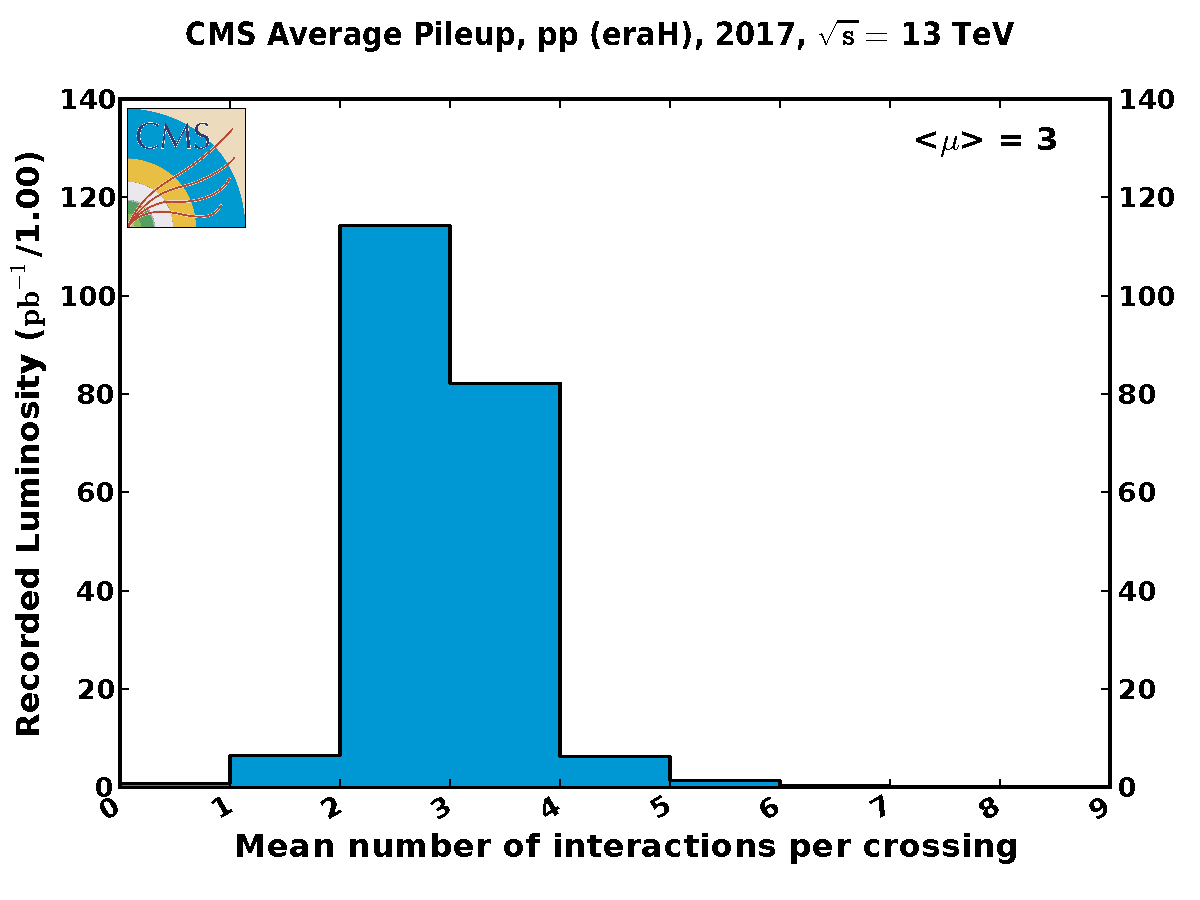
\includegraphics[width=0.75\textwidth]{plots/Data/pileup_pp_lowPU_2017.pdf}
  %https://cds.cern.ch/record/40524
  \caption{Distribution of the number of interactions per bunch crossing for the low pileup \sh (2017H) data taking period. The average number of interactions per crossing is $<\mu> = 3$~\cite{LumiCalibTwiki}.}
  \label{fig:data:lumiPU13}
\end{figure}

\begin{figure}[htbp]
\centering
  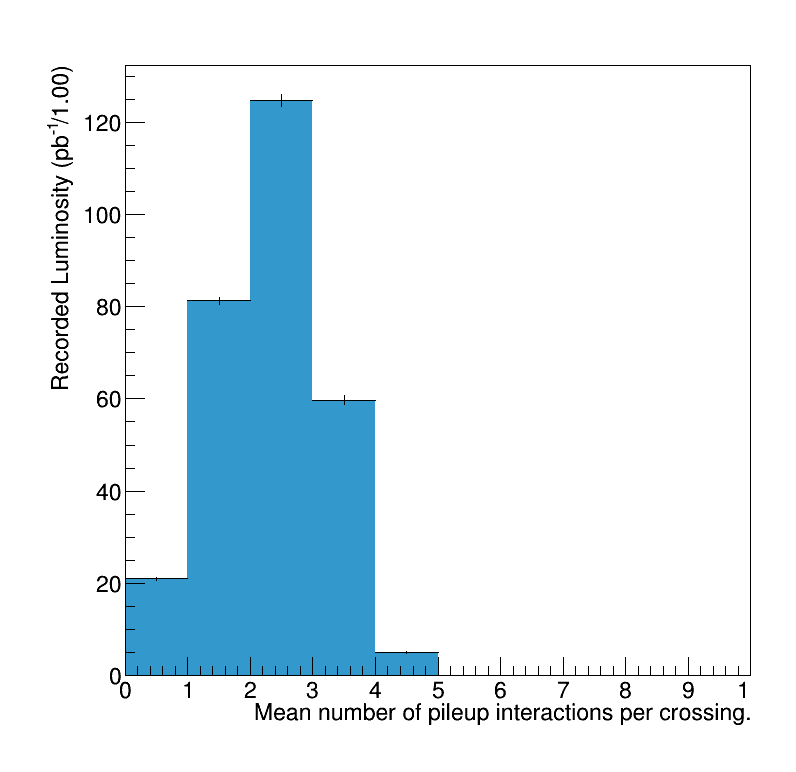
\includegraphics[width=0.75\textwidth]{plots/Data/pileup_5TeV.png}
  %https://cds.cern.ch/record/40524
  \caption{Distribution of the number of interactions per bunch crossing for the \sg (2017G) data taking period. The average number of interactions per crossing is $<\mu> = 2$~\cite{LumiCalibTwiki}.}
  \label{fig:data:lumiPU5}
\end{figure}
\begin{figure}[htbp]
\centering
  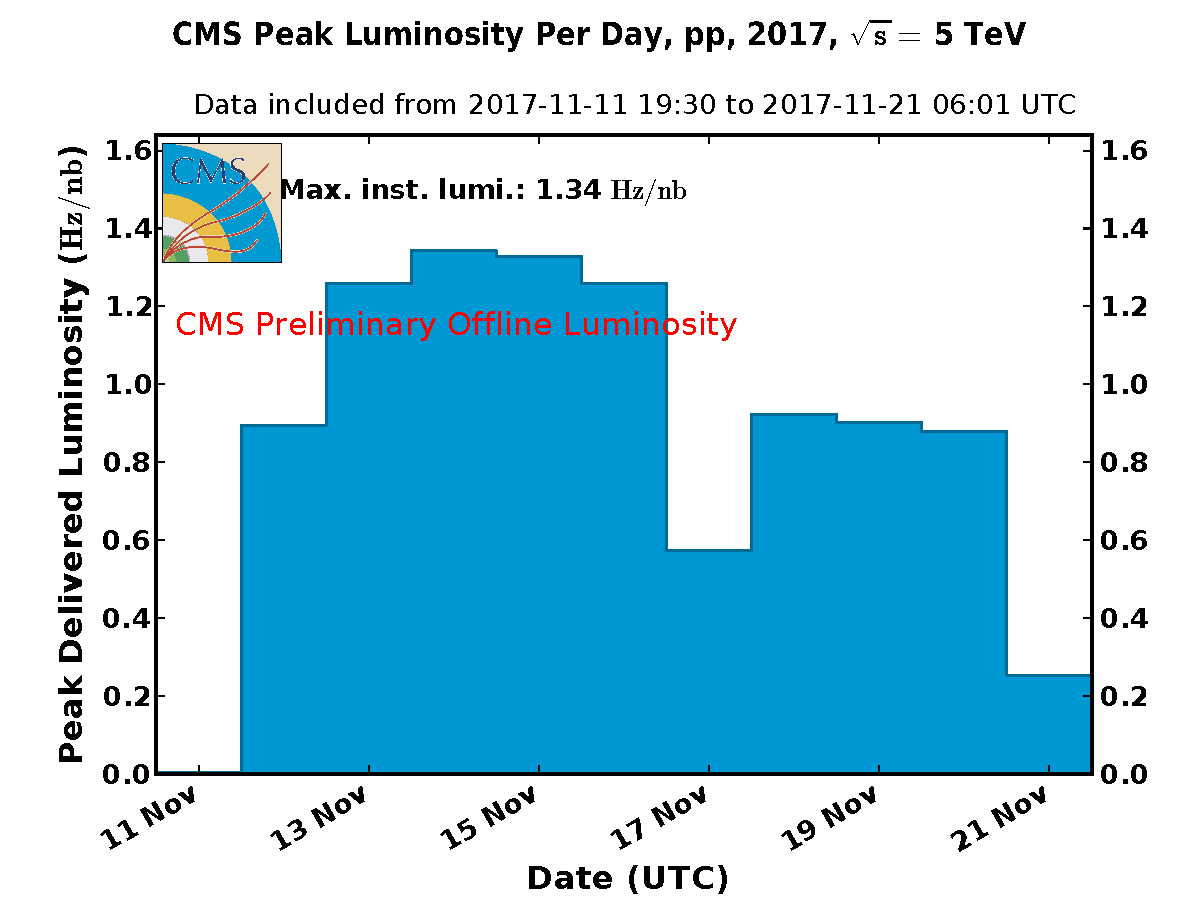
\includegraphics[width=0.6\textwidth]{plots/Data/peak_lumi_per_day_pp_2017_5TeV_NormtagLumi.pdf}
  %https://cds.cern.ch/record/40524
  \caption{Peak instantaneous luminosity per day during the \sg (2017G) data taking period~\cite{LumiCalibTwiki}.}
  \label{fig:data:lumiperday5}
\end{figure}
%%%% lumi values
\begin{table}[htbp]
\begin{center}
\scalebox{1.0}{
\begin{tabular}{c c c}
\hline {\s [\TeV]} & {Run Era} &  {Luminosity [\invpb]}  \\
\hline \hline
5.02  & 2017G    &   $199.2 \pm   3.39$   \\
13    & 2017H    &   $291.1 \pm  11.64$   \\
\hline
\end{tabular}}
\end{center}

\caption{Datasets and their respective integrated luminosity measurements.}
\label{tab:lumis}
\end{table}

%% Is there a specific thing to cite if you use brilcalc to get the lumi out of the trigger path


%%%%%%%%%%%%%%%%%%%%%%%%%%%%%%%%%%%%%%
%%%     Simulated Samples & info 
%%%%%%%%%%%%%%%%%%%%%%%%%%%%%%%%%%%%%%

\section{Simulated samples}\label{ch:data:sim}
Several simulated Monte Carlo (MC) samples are used in the descriptions of signal and background processes. The \Wpm and \Z boson signal events are simulated at next-to-leading order (NLO) with up to two outgoing partons at Born level by \MGvATNLO~2.3.3~\cite{Alwall:2014hca}. An additional set of simulations of the \Wpm and \Z boson signal processes are provided at NLO by \POWHEG~2.0~\cite{Alioli:2008gx,Frixione:2007vw,powheg:2010,Alioli:2010xd} for the \Wpm and \MINLO~\cite{Hamilton:2012rf} for the \Z boson. Background samples (di-boson and \ttbar) are also simulated with \POWHEG~2.0. Underlying event modeling, parton showering, hadronization, and final state radiation are done by \PYTHIA~8.230~\cite{Sjostrand:2014zea}, using tune CP5~\cite{Sirunyan:2019dfx} and default parton distribution functions (PDFs) provided by NNPDF3.1~\cite{Ball:2017nwa}. Primary sample names and their respective production cross sections are listed in Table~\ref{tab:allSamples5} (Table~\ref{tab:allSamples13}) for \serag (\serah).

The distribution of pileup interactions is simulated to match the corresponding conditions in data. For all simulated samples, simulation of detector response is performed by \GEANTfour~\cite{Agostinelli:2002hh}, with full event reconstruction being done using the same algorithms used to reconstruct data. Object and event reconstruction was described in Chapter~\ref{ch:reco}. 

%%% 5 TeV MCs
\begin{table}[htbp]
\begin{center}
\scalebox{0.9}{
\begin{tabular}{llr}
\hline
{Sample name} & {Generator} &{~~~Cross section~[pb]} \\
\hline \hline
W+Jets & \aMCATNLO & 21159 \\
\hline
$WW\to 2\ell 2\nu$  & \POWHEG & 2.52 \\
$WZ\to 3\ell \nu$  & \POWHEG & 1.23 \\
$ZZ\to 4\ell$  & \POWHEG & 2.75 \\
$ZZ\to 2\ell 2\nu$  & \POWHEG & 2.75 \\
\hline
\ttbar  & \POWHEG &  69.5 \\
\hline
DY+jets$\to\ell\ell$ ~~~ & \aMCATNLO & 2141  \\
\hline
\end{tabular}}
\end{center}
\caption{Names and cross sections of simulated samples corresponding to run era 2017G (\serag).}
\label{tab:allSamples5}
\end{table}


%%% 13 TeV MCs
\begin{table}[htbp]
\begin{center}
\scalebox{0.9}{
\begin{tabular}{llr}
\hline
{Sample name}  & {Generator}& {~~~Cross section~[pb]} \\
\hline \hline
$W$+0 jets & \aMCATNLO & 49397\\
$W$+1 jets  &\aMCATNLO & 8087 \\
$W$+2 jets  & \aMCATNLO & 3176 \\
\hline
ZZ  & \POWHEG  & 16.523 \\
$WZ\to 3\ell\nu$  & \POWHEG  & 4.912 \\
$WZ\to 2\ell 2\nu$  & \POWHEG  & 12.6 \\
\hline
$\ttbar \to 2\ell 2\nu$  & \POWHEG  & 88.29 \\
$\ttbar \to \mathrm{semileptonic}$ ~~~ & \POWHEG  & 365.35 \\
$\ttbar \to \mathrm{hadronic}$  & \POWHEG  & 377.96 \\
\hline
DY+jets$\to\ell\ell$  & \aMCATNLO & 6225.42 \\
\hline
\end{tabular}}
\end{center}
\caption{Names and cross sections of simulated samples corresponding to run era 2017H (\serah).}
\label{tab:allSamples13}
\end{table}



% %%% 5 TeV MCs
% \begin{table}[htbp]
% \begin{center}
% \scalebox{0.9}{
% \begin{tabular}{lrr}
% \hline
% {Sample name} & {Cross section~[pb]} \\
% \hline \hline
% WJetsToLNu\_TuneCP5\_5020GeV-amcatnloFXFX-pythia8 & 21159 \\
% \hline
% WWTo2L2Nu\_NNPDF31\_TuneCP5\_5p02TeV-powheg-pythia8 & 2.52 \\
% WZTo3LNU\_NNPDF30\_TuneCP5\_5p20TeV-powheg & 1.23 \\
% ZZTo4L\_5p02TeV\_powheg\_pythia8 & 2.75 \\
% ZZTo2L2Nu\_5p02TeV\_powheg\_pythia8 & 2.75 \\
% \hline
% TT\_TuneCP5\_5p02TeV-powheg-pythia8 &  69.5 \\
% \hline
% DYJetsToLL\_MLL-50\_TuneCP5\_5020GeV-amcatnloFXFX-pythia8 & 2141  \\
% \hline
% \end{tabular}}
% \end{center}
% \caption{Names and cross sections of simulated samples corresponding to run era 2017G (5.02 TeV).}
% \label{tab:allSamples5}
% \end{table}


% %%% 13 TeV MCs
% \begin{table}[htbp]
% \begin{center}
% \scalebox{0.9}{
% \begin{tabular}{lrr}
% \hline
% {Sample name} & {Cross section~[pb]} \\
% \hline \hline
% WJetsToLNu\_0J\_TuneCP5\_13TeV-amcatnloFXFX-pythia8 & 49397\\
% WJetsToLNu\_1J\_TuneCP5\_13TeV-amcatnloFXFX-pythia8 & 8087 \\
% WJetsToLNu\_2J\_TuneCP5\_13TeV-amcatnloFXFX-pythia8 & 3176 \\
% \hline
% ZZ\_TuneCP5\_13TeV-pythia8  & 16.523 \\
% WZTo3LNu\_TuneCP5\_13TeV-powheg-pythia8  & 4.912 \\
% WWTo2L2Nu\_TuneCP5\_13TeV-powheg-pythia8  & 12.6 \\
% \hline
% TTTo2L2Nu\_TuneCP5\_13TeV-powheg-pythia8  & 88.29 \\
% TTToSemiLeptonic\_TuneCP5\_13TeV-powheg-pythia8  & 365.35 \\
% TTToHadronic\_TuneCP5\_13TeV-powheg-pythia8  & 377.96 \\
% \hline
% DYJetsToLL\_M-50\_TuneCP5\_13TeV-amcatnloFXFX-pythia8 & 6225.42 \\
% \hline
% \end{tabular}}
% \end{center}
% \caption{Names and cross sections of simulated samples corresponding to run era 2017H (13 TeV).}
% \label{tab:allSamples13}
% \end{table}




%%%%%%%%%%%%%%%%%%%%%%%%%%%%%%%%%%%%%%
%%%     Event Selection
%%%%%%%%%%%%%%%%%%%%%%%%%%%%%%%%%%%%%%
\section{Event Selection \& Fiducial Region}
 \subsubsection{Reconstructed}
Preliminary \Wpm and \Z boson event candidates are identified by the presence of at least one lepton identified by the single electron and single muon triggers described in Section~\ref{ch:data:triggers}. These are further selected by applying the offline electron or muon reconstruction identification criteria described in Section~\ref{ch:IdIso}. 
A \Z boson event requires the presence a pair of oppositely charged leptons ($e^{+}e^{-}$ or $\mu^{+}\mu^{-}$), at least one of the leptons being identified by the trigger, and each of the leptons fulfilling the ID requirements in Section~\ref{ch:IdIso}, and an invariant mass of \masswindow. 
Selection of a \Wp or \Wm boson candidate requires one charged lepton identified by the trigger and passing all ID requirements in Section~\ref{ch:IdIso}. A veto is applied to events containing additional leptons passing a loose identification requirement. 

% Additionally, \Wpm events are required to have an invariant mass $\mt > 40\GeV$, with \mt defined by: 
% $\mt = \sqrt{ 2 \pt \met ( 1 - \cos(\Delta\phi) ) }$, where $\Delta\phi$ is the angle between the lepton and \vmet in the transverse plane.

\subsubsection{Fiducial Region}
The fiducial region for the \Wpm and \Z boson acceptance at generator-level emulates the selection at reconstruction level. This requires kinematic cuts $\pt > 25 \GeV$ and $|\eta| < 2.4$ for all charged leptons. Additionally, the \Z boson fiducial region includes a requirement on the dilepton mass: \masswindow. The fiducial region for the \W boson includes the transverse mass requirement $\mt>40\GeV$.


%%%%%%%%%%%%%%%%%%%%%%%%%%%%%%%%%%%%%%
%%%     object definition
%%%%%%%%%%%%%%%%%%%%%%%%%%%%%%%%%%%%%%
\section{Object Identification}\label{ch:IdIso}
The \W and \Z boson candidates are identified by the presence of one or two, respectively, well-identified leptons passing a strong set of criteria ensuring proper reconstruction and identification. This section contains a description of the identification requirements for the \wlnu and \zll signal leptons, as well as the requirements for the lepton veto for the \Wpm boson selection.

\subsection{Isolation}\label{ch:id:iso}
One of the most important observables used to separate the leptons from \Wp and \Wm boson events from QCD background is the isolation. Isolated leptons have little other activity within a cone of $\Delta R < 0.3$, and leptons from \wlnu decays are generally isolated. The isolation of a lepton is constructed from the sum of all charged and neutral hadrons and ECAL deposits within $\Delta R < 0.3$ of the lepton, as shown in Equation~\ref{eq:pfiso}. 
\begin{equation}
    I_{PF} = \frac{1}{\pt}\sum_{\Delta R<0.3}( \pt^{h^0} + \pt^{h^\pm} +  \pt^{\gamma})
    \label{eq:pfiso}
\end{equation}
The individual contributions to the PF isolation are the sums of corresponding particle types which fall within a cone of $\Delta R < 0.4$.
% \begin{equation}
%     \Delta R = \sqrt{\Delta\eta^2+\Delta\phi^2}
%     \label{eq:dR}
% \end{equation}
% Neutral particle contributions due to pileup are estimated by computing charged hadron contributions from pileup vertices and scaling it by 0.5. The scaling factor was determined using simulation. This pileup contribution is subtracted from the total neutral particle energy sum to get the neutral particle isolation, which is limited to be $\geq0$.

\subsection{Electrons}\label{ch:IdIso:Ele}
Electrons originating from candidate \Wp, \Wm, and \Z bosons are required to pass the standard cut-based identification with medium working point. Backgrounds producing electron-like signatures include overlapping charged and neutral pions, pions showering in the ECAL, and jets, and the selection criteria are designed to exclude these. The thresholds for observables required to pass this requirement are listed in Table~\ref{tab:Data:Sel:Ele} Descriptions of the observables are provided below. The \Wpm boson selection requires the absence of additional leptons in the event. The veto is performed with leptons fulfilling the loose working point identification requirements, with criteria for electrons listed in Table~\ref{tab:Data:Sel:EleVeto}. 
%~\cite{EgammaIDIsoCuts}.
\subsubsection{Electron Observables}
\begin{itemize}
    \item \textbf{($\Delta\eta_{In}$,$\Delta\phi_{In}$):} Geometric matching of the ECAL supercluster and electron GSF track, extrapolated to the vertex. Real electrons are well-matched since they come from the same object. 
    \item \textbf{$\sigma_{i\eta i\eta}$:} Shape of the shower in the ECAL. Electrons can be discriminated from jets by the evolution of the shower in the 5x5 crystal region around the seed.
    \item \textbf{H/E:} Ratio of energy deposited in HCAL to ECAL. Electrons tend to deposit most of their energy in the ECAL, while jets deposit substantial amounts their of energy in the HCAL.
    \item \textbf{$|d_{0,bs}|$,~$|d_{z,bs}|$:} Impact parameters are defined as the distance of closest approach of the track to the vertex. Requiring an impact parameter cut removes electrons from displaced vertices.
    \item \textbf{$|1/E-1/p|$:} Electron energy measured in ECAL is compatible with momentum measured in tracker.
    \item \textbf{Number of Missing Hits}: Number of missing tracker hits in tracker layer
    \item \textbf{Isolation:} Requiring that electrons be isolated reduces the number of jets reconstructed as electrons.
    \item \textbf{Conversion probability}: Photons converting to electron-positron pairs are a source of isolated electrons. Electrons from photon conversion are identified by fitting $e^+e^-$ pairs to a common vertex.
\end{itemize}

%%%% Table containing the Ele ID+Iso cuts
\begin{table}[htbp]
\begin{center}
\scalebox{0.8}{
\begin{tabular}{|c|c|c|}
\hline
Observable & Barrel & Endcap \\
\hline \hline
$p_T$ & \multicolumn{2}{c|}{$> 25$ \GeV} \\ \hline % OK
$|\eta|$ & \multicolumn{2}{c|}{$< 2.4$}\\ \hline% OK
$\Delta\eta_{In}$ & $< 0.0032$ & $< 0.00632$\\ \hline% OK
$\Delta\phi_{In}$ & $< 0.0547$ & $< 0.0394$\\ \hline% OK
$\sigma_{i\eta i\eta}$ & $<  0.0106$ & $< 0.0387$\\ \hline% OK
H/E & $< 0.046+1.16/E_{SC}+0.0324\rho/E_{SC}$ & $< 0.0275+2.52/E_{SC}+0.183\rho/E_{SC}$\\ \hline%
$|d_{0,bs}|$ & $< 0.05$ & $< 0.10$\\ \hline% OK
$|d_{z,bs}|$ & $< 0.10$ & $< 0.20$\\ \hline% OK
$|1/E-1/p|$ & $< 0.184$& $< 0.0721$\\ \hline% OK
$\mathrm{Iso_{PF}}/$\pt &$< 0.0478+0.506/p_{\mathrm{T},ele}$ &$< 0.0658+0.963/p_{\mathrm{T},ele}$ \\ \hline
Missing Hits & \multicolumn{2}{c|}{$\leq 1$}\\ \hline
\multicolumn{3}{|c|}{Pass conversion veto}\\
\hline
\end{tabular} }
\end{center}
\caption{Reconstructed identification and isolation criteria fulfilling the medium cut-based ID for electron selection.}
\label{tab:Data:Sel:Ele}
\end{table}

%% Table containing the Electron ID+Iso Veto cuts
%% Cut Type
\begin{table}[htbp]
\begin{center}
\scalebox{0.8}{
\begin{tabular}{|c|c|c|} %%%% Table needs vertical lines
\hline
Observable & Barrel & Endcap \\
\hline \hline
$p_T$ & \multicolumn{2}{c|}{$> 25$ \GeV} \\ \hline % OK
$|\eta|$ & \multicolumn{2}{c|}{$< 2.4$}\\ \hline% OK
$\Delta\eta_{In}$ & $< 0.00463$ & $< 0.00814$\\ \hline
$\Delta\phi_{In}$ & $< 0.148$ & $< 0.19$\\ \hline
$\sigma_{i\eta i\eta}$ & $< 0.0126$ & $< 0.0457$\\ \hline
H/E & $< 0.05+1.16/E_{SC}+0.0324\rho/E_{SC}$ & $< 0.05+2.54/E_{SC}+0.183\rho/E_{SC}$\\ \hline%
$|d_{0,bs}|$ & $< 0.05$ & $< 0.10$\\ \hline
$|d_{z,bs}|$ & $< 0.10$ & $< 0.20$\\ \hline
$|1/E-1/p|$ & $<0.209$& $< 0.132$\\ \hline
$\mathrm{Iso_{PF}}/$\pt &$< 0.198+0.506/p_{T,ele}$ &$< 0.203+0.963/p_{T,ele}$ \\ \hline
Missing Hits & $\leq 2$ & $\leq 3$\\ \hline
\multicolumn{3}{|c|}{Pass conversion veto}\\
\hline
\end{tabular}}
\end{center}
\caption{Reconstructed identification and isolation criteria fulfilling the loose cut-based ID for electron selection used as a veto on \Wpm events with additional leptons present.}
\label{tab:Data:Sel:EleVeto}
\end{table}

\subsection{Muons}\label{ch:IdIso:Mu}
Muons originating from a candidate \Wpm or \Z boson are required to pass the standard cut-based identification with tight working point with tight working point requirement on the muon PF isolation. The thresholds for observables required to pass this requirement are listed in Table~\ref{tab:Data:Sel:Mu}.Descriptions of the observables are provided below. As in the electron channel, the \Wpm boson selection requires the absence of additional leptons in an event which pass the loose cut-based ID. The criteria for muons is listed in Table~\ref{tab:Data:Sel:Mu:Veto}. 
%~\cite{MuonIDIsoCuts}. 
% do i even need citation

%%%%%%%%%%%%%%%%%%%%%%%%%%%%%%%%%%%%%
\subsubsection{Muon Observables}
\begin{itemize}
    \item \textbf{Global Muon \& PF Muon:} Muon candidate is successfully reconstructed by these algorithms
    \item \textbf{$\chi^2/$ndof:} Quality of the muon track fit, require convergence of the fit.
    \item \textbf{Number of Valid Hits:} Number of muon system hits included in the global muon reconstruction. Global muons rarely have 0 valid hits.
    \item \textbf{Number of Matched Stations:} Number of muon segments in the muon stations
    \item \textbf{Number of Pixel Hits:} Activity in the pixel tracker associated with the muon removes muons from backgrounds such as cosmic rays and decay-in-flight of pions and kaons. 
    \item \textbf{Number of Tracker Hits:} Similar to the pixel tracker requirements, the total number of tracker hits can further reduce backgrounds from decay-in-flight.
    \item \textbf{$|d_{0,bs}|$,~$|d_{z,bs}|$:} Impact parameters $d_0$ and $d_z$ are defined as the distance of closest approach of a track to the primary interaction vertex. Removes muons from displaced vertices and cosmic rays. 
    \item \textbf{Isolation:} Muons originating from heavy flavor decays often have other leptons and light mesons nearby, and are therefore less isolated.
\end{itemize}

%%%% Table containing the Ele ID+Iso cuts
\begin{table}[htbp]
\begin{center}
\scalebox{0.8}{
\begin{tabular}{|c|c|}
\hline
Observable & Value/Range \\
\hline \hline
\pt & > 25 GeV \\ \hline % OK
$|\eta|$ & $< 2.4$\\ \hline% OK
ID & ~GlobalMuon~ \\ \hline% OK
ID & ~PFMuon~\\ \hline% OK
$\chi^2/$ndof & $< 10$\\ \hline% OK
~\# Valid Mu Hits ~ & $\geq 1$\\ \hline%
~\# Matched Stations ~& $\geq 2$\\ \hline%
~\# Tracker Layers ~& $\geq 6$\\ \hline%
~\# Valid Pixel Hits~ & $\geq 1$\\ \hline%
$|d_{0,bs}|$ & < 0.2 \\ \hline% OK
$|d_{z,bs}|$ & < 0.5 \\ \hline% OK
$\mathrm{Iso_{PF}}/$\pt &$< 0.15$\\
\hline
\end{tabular}}
\end{center}
\caption{Reconstructed identification and isolation criteria fulfilling the cut-based ID with tight isolation requirement for muon selection.}
\label{tab:Data:Sel:Mu}
\end{table}
%%%% Table containing the Ele ID+Iso cuts
\begin{table}[htbp]
\begin{center}
\scalebox{0.8}{
\begin{tabular}{|c|c|c|}
\hline
Observable & Value/Range \\
\hline \hline
\pt & > 10 GeV \\ \hline % OK
$|\eta|$ & < 2.4\\ \hline% OK
ID & \textsc{GlobalMuon} \textbf{OR} \textsc{TrackerMuon}\\ \hline% OK
ID & \textsc{PFMuon}\\ 
\hline
\end{tabular}}
\end{center}
\caption{Reconstructed identification and isolation criteria for identifying additional muons used as a veto on \Wpm boson events.}
\label{tab:Data:Sel:Mu:Veto}
\end{table}


\chapter{Lepton Efficiency Scale Factors}\label{ch:eff}
The efficiency of the trigger and reconstruction and identification steps for leptons is non-unity and differs between simulation and data. Determining the efficiency of the reconstruction and identification workflow separately for simulation and data provides a scale factor $\epsilon_{data}/\epsilon_{MC}$ for each lepton to effectively match the reconstruction efficiency of simulation to data. Efficiency scale factors are derived over the fiducial region with fine enough granularity to separate behavior in different kinematic regions and detector geometry. The scale factor is applied to the simulated signal and background samples to emulate the lepton reconstruction and identification efficiency expected in data.

% The overall impact of the efficiencies on the W signal provides the expected W signal event yield in the dataset, as shown in Equation~\ref{eq:W_eff}. 

% \begin{equation}
%   \epsilon_{W,data} = \epsilon_{W,MC}\times\frac{\epsilon_{tot,data}}{\epsilon_{tot,MC}}
%   \label{eq:W_eff}
% \end{equation}
The factorization of the efficiency effects for electrons is shown in Equation~\ref{eq:ele_eff}. $\epsilon_{GSF+ID+Iso}$ is the efficiency of creating an ECAL-driven GSF electron that also passes the electron identification and isolation criteria, as described in Table~\ref{tab:Data:Sel:Ele}. $\epsilon_{HLT}$ describes the efficiency of a GSF electron passing the identification and isolation requirements to also be selected by the HLT. 

\begin{equation}
  \epsilon_{e} = \epsilon_{GSF+ID+ISO} \times \epsilon_{Trigger}
  \label{eq:ele_eff}
\end{equation}
\begin{equation}
  \epsilon_{\mu} = \epsilon_{ID+ISO+Trk} \times  \epsilon_{Sta} \times \epsilon_{Trigger}
  \label{eq:mu_eff}
\end{equation}

Likewise, the factorization for the muon efficiency factors is shown in Equation~\ref{eq:mu_eff}. $\epsilon_{ID+Iso+Trk}$ is the efficiency of a standalone muon to be matched with a global muon being matched to tracker hits and satisfying the identification and isolation criteria (listed in Table~\ref{tab:Data:Sel:Mu}). $\epsilon_{Sta}$ is the efficiency for a global muon to be matched to the standalone muon system and 
$\epsilon_{Trigger}$ is the efficiency with which a fully identified and isolated muon is selected by the HLT. 


% %%%% Tables for Electron Efficiency SF Uncertainty for 13 TeV  %%%%%
\begin{table}%[htbp]
\begin{center}
\scalebox{0.7}{
\begin{tabular}{ccccc}
\hline
Probe Type & Tag Type & $\eta$ bins & $p_T$ bins & Charge bins \\
\hline \hline
GSF+Selection+Iso & sc  & 12 &  8 & charge-inclusive\\
Trigger & GSF electron  & 12 &  8  & +, -\\
\hline
\end{tabular}}
\end{center}
\caption{General implementation of the electron scale factor derivation. Both sets of scale factors are derived for $e^+$ and $e^-$ separately. }
\label{tab:Eff:Binning:Ele}
\end{table}

% %%%% Tables for Electron Efficiency SF Uncertainty for 13 TeV  %%%%%
\begin{table}%[htbp]
\begin{center}
\scalebox{0.7}{
\begin{tabular}{ccccc}
\hline
Probe Type & Tag Type & $\eta$ bins & $p_T$ bins & Charge bins\\
\hline \hline
Sel+ID+Iso & 0.00  & 12 &  3 &charge-inclusive\\
Standalone & 0.00  & 12 &  3  & charge-inclusive\\
Trigger & 0.00  & 12 &  8  & +, -\\
\hline
\end{tabular}}
\end{center}
\caption{General implementation of the muon scale factor derivation. Standalone efficiency has fewer $pT$ bins due to the low $p_T$ dependence and having a stastically limited fit in the failing probe category.}
\label{tab:Eff:Binning:Mu}
\end{table}



%% %%%%%%%%%%%%%%%%%%%%%%%%%%%
%%                Tag & Probe
%%%%%%%%%%%%%%%%%%%%%%%%%%%%%
\section{Tag and Probe}\label{ch:eff:tagandprobe}
A tag-and-probe method is employed on the \zll sample, which provides a high-purity sample of high-\pt leptons which have similar kinematic properties to those also present in the leptonic \W boson decays\cite{Khachatryan:2010xn}. Tag leptons are leptons passing the cut-based lepton ID requirements as described in Section~\ref{ch:IdIso} as well as being matched to the appropriate trigger object. Probe leptons are then selected from leptons passing the loose kinematic cuts of $p_T > 25 \mathrm{~GeV}$,~$|\eta|<2.4$, and producing a dilepton invariant mass in the range \masswindow. Probes are classified by their ability to pass a set of criteria depending on the efficiency being studied. Calculation of the efficiency is described in Section~\ref{ch:eff:fitting}.

Lepton efficiencies are calculated based on the probe \pt and $\eta$. Binning by $\eta$ is listed in Table~\ref{tab:eff:bin:eta} and binning by $\pt$ is listed in Table~\ref{tab:eff:bin:pt}. Identical $(\pt,\eta)$ binning is used at \serag and \serah for a given category. The trigger efficiency for all channels is derived with positively and negatively charged categories separated, while the charges are combined for the other categories. Electron efficiency $\eta$ binning includes a category specifically to accommodate the gap between the endcap and barrel which contains a large amount of inactive material and has a significantly lower efficiency than other areas.
%%%% Tables for Electron Efficiency SF Uncertainty for 13 TeV  %%%%%
\begin{table}[htbp]
\begin{center}
\scalebox{0.9}{
\begin{tabular}{cc}
\hline
Channel~~ & $\eta$ bins \\
\hline \hline
Muon  & -2.4, -2.1, -1.6, -1.2, -0.9, -0.3, 0, 0.3, 0.9, 1.2, 1.6, 2.1, 2.4  \\
Electron  & -2.4, -2.0, -1.566, -1.4442, -1.0, -0.5, 0, 0.5, 1.0, 1.4442, 1.566, 2.0, 2.4 \\
\hline
\end{tabular}}
\end{center}
\caption{$\eta$ binning used for each lepton channel. }
\label{tab:eff:bin:eta}
\end{table}

%%%% Tables for Electron Efficiency SF Uncertainty for 13 TeV  %%%%%
\begin{table}[htbp]
\begin{center}
\scalebox{0.9}{
\begin{tabular}{ccc}
\hline
Category & ~Channel~ & \pt bins [\GeV] \\
\hline \hline
Trigger & electron, muon ~~`& 25, 26.5, 28, 29.5, 31, 32.5, 35, 40, 45, 50, 60, 80, $\infty$ \\
\hline
GSF+ID+Iso & electron  \\
Standalone & muon &  25, 35, 50, $\infty$ \\
Selection+Iso & muon &  \\
\hline
\end{tabular}}
\end{center}
\caption{\pt binning used for each efficiency category. }
\label{tab:eff:bin:pt}
\end{table}


% Category & ~~~$\ell$~~~ & \pt bins [\GeV] \\
% \hline \hline
% Trigger & $e, \mu$ & 25, 26.5, 28, 29.5, 31, 32.5, 35, 40, 45, 50, 60, 80, $\infty$ \\
% \hline
% GSF+ID+Iso & $e$ &  \\
% Standalone & $\mu$ &  25, 35, 50, $\infty$ \\
% Selection+Iso & $\mu$ &  \\



%% %%%%%%%%%%%%%%%%%%%%%%%%%%%
%%                Fitting
%%%%%%%%%%%%%%%%%%%%%%%%%%%%%

\section{Fitting Method}\label{ch:eff:fitting}
Probes are categorized into a "pass" and "fail" category for each kinematic bin of the efficiency type being studied. The number of passing and failing $Z\rightarrow ll$ events determine the efficiency as shown in Equation~\ref{eq:eff:eq}. For simulated samples, which are pure \zll, $N_{pass}$ and $N_{fail}$ can be determined by counting the number of events in each category per bin. 

\begin{equation}
\epsilon = \frac{N_{pass}}{N_{pass}+N_{fail}}
\label{eq:eff:eq}
\end{equation}
Data, in particular the probes in the "fail" category, may also include background events in addition to the \zll signal events. To determine $N_{pass}$ and $N_{fail}$ in data, a fit is performed to discriminate between \zll events and other backgrounds. The \zll events are modeled using the Monte Carlo distribution smeared with a Gaussian. Backgrounds are modeled using a simple function which is varies based on efficiency category. The specific background models are described in Section~\ref{ch:eff:bkg}.


The events in the category of $\epsilon_{HLT}$ have negligible background, and $\epsilon$ is determined by counting events in the "pass" and "fail" categories.
After construction of the signal and background models, the passing and failing categories for a given kinematic bin are simultaneously fit with Equations~\ref{eq:eff:pass:full} and~\ref{eq:eff:fail:full} to extract $\epsilon$. Examples of the fit are shown in Figure~\ref{fig:eff:musta:fitexample}.

\begin{equation}
F^{pass}\left(m_{ll}\right)=\epsilon \times N_{tot} \times F_{sig}^{pass}\left(m_{ll} \right) + N^{pass}_{bkg} \times F_{bkg}^{pass} \left(m_{ll} \right)
\label{eq:eff:pass:full}
\end{equation}
\begin{equation}
F^{fail}\left(m_{ll}\right)=\left(1-\epsilon\right) \times N_{tot} \times F_{sig}^{fail}\left(m_{ll} \right) + N^{fail}_{bkg} \times F_{bkg}^{fail} \left(m_{ll} \right)
\label{eq:eff:fail:full}
\end{equation}





%% %%%%%%%%%%%%%%%%%%%%%%%%%%%
%%                Systematics
%%%%%%%%%%%%%%%%%%%%%%%%%%%%%
\section{Modeling and Systematic Uncertainties}\label{ch:eff:systematics}
Uncertainties in the efficiency factors is evaluated for sources including signal model choice, background model choice, and tag selection. The variations in the scale factors is propagated to the discrminant distributions used in the final fit.
\subsection{Evaluating Model Differences}
Uncertainties in the scale factors are evaluated as coming from model-dependence of results on the signal and background shapes. These include the FSR model, generator, and background model. Additionally, the impact of the minimum tag selection \pt is evaluated. 
The impact of the model assumptions is evaluated by generating a set of simulated datasets from the \mll distribution describing the original efficiency model and fitting with the alternative models. The pull, $ (\epsilon_{meas}-\epsilon_{true})/{\sigma_{meas}} $, for each trial is calculated, and the mean pull per \pt-$\eta$ bin is taken to be the uncertainty due to the alternate model. 
% \begin{equation}
% \mathrm{pull}=\frac{\epsilon_{meas}-\epsilon_{true}}{\sigma_{meas}}
%     \label{eq:ch7:pull}
% \end{equation}

\subsubsection{Generator Model}
\textbf{\aMCATNLO vs. \POWHEG:} The primary signal simulation for this analysis is \\\aMCATNLO with \PYTHIA8.2. The matrix element calculation is done with \MADGRAPH5\_\aMCATNLO with NNPDF3.1 PDF sets. To account for the assumptions and approximations specific to this model, alternative samples generated with \POWHEG and \PYTHIA8.2 are used. Generator-level information from the \POWHEG sample is used to create alternative reconstructed \mll distributions from simulation. New fit models are created from the \POWHEG \mll distributions convolved with a Gaussian.

\subsubsection{Final-State Radiation Model}
\textbf{\PYTHIA vs. \PHOTOS:} Final state radiation for the main set of simulations is performed by \PYTHIA8.2. Evaluation of the FSR model choice is done by comparing \PYTHIA against the \PHOTOS model. As with the generator model uncertainty evaluation, new fit models are created from the \PHOTOS \mll distributions convolved with a Gaussian.

\subsubsection{Background Model}\label{ch:eff:bkg}
Simulated datasets are generated from the primary fit models, and alternatives containting different background functions are used to fit. The baseline corrections are derived with the background models: 
\begin{itemize}
\item \textbf{exponential} for muon selection+ID+Isolation efficiency
\item \textbf{exponential $\otimes$ erf} for electron GSF ID+Isolation efficiency (where erf is the Gauss error function)
\item \textbf{quadratic polynomial} for muon standalone efficiency
\end{itemize}
The alternate set of fitting functions is constructed with:
\begin{itemize}
\item \textbf{power law} for alternative model in all categories
\end{itemize}
Examples of a muon standalone efficiency fit using the standard quadraditc function and the alternative power law model are shown in Figure~\ref{fig:eff:musta:fitexample}. 
%%%% Figures for ZeeGSFSel Efficiency  %%%%%
\begin{figure}
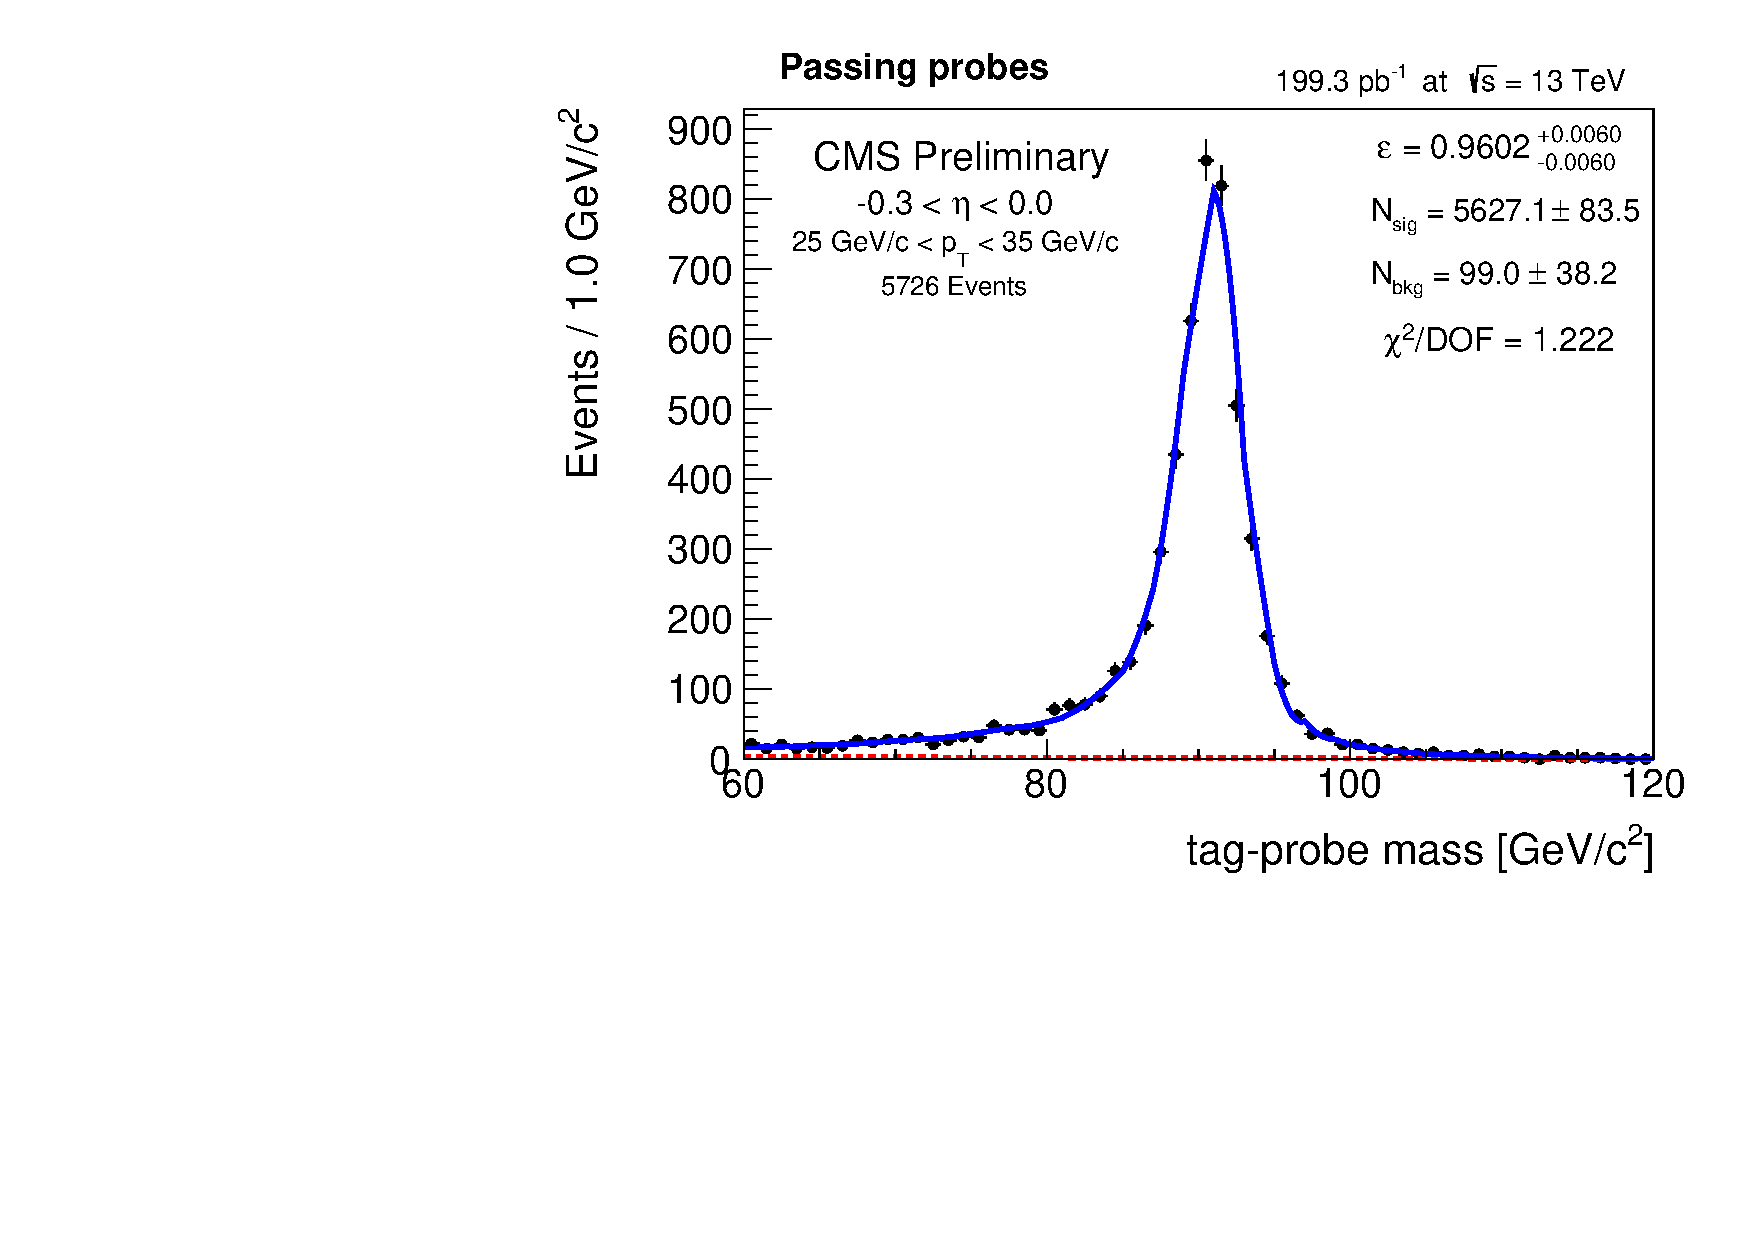
\includegraphics[width=.49\linewidth]{plots/efficiency/examples_musta/passetapt_5.pdf}
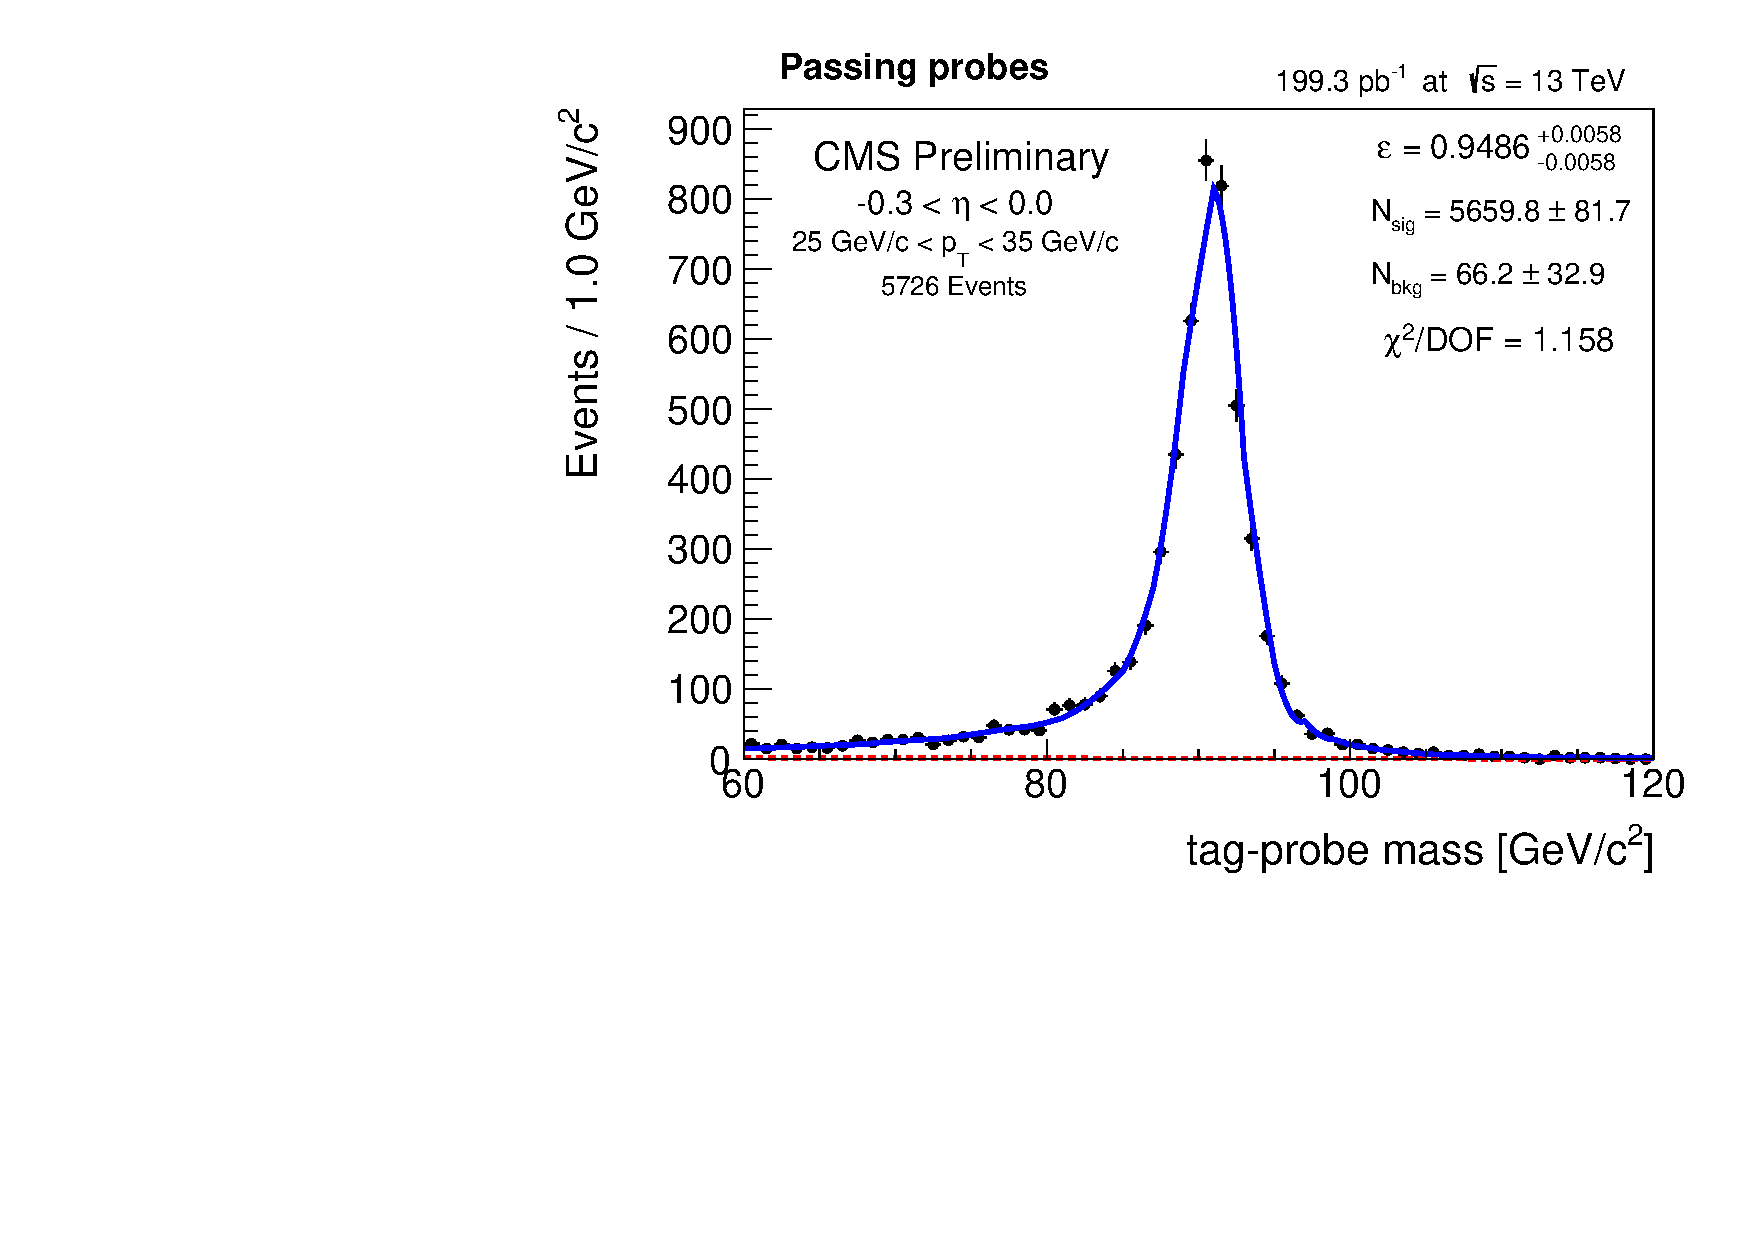
\includegraphics[width=.49\linewidth]{plots/efficiency/examples_plbkg/passetapt_5.pdf}
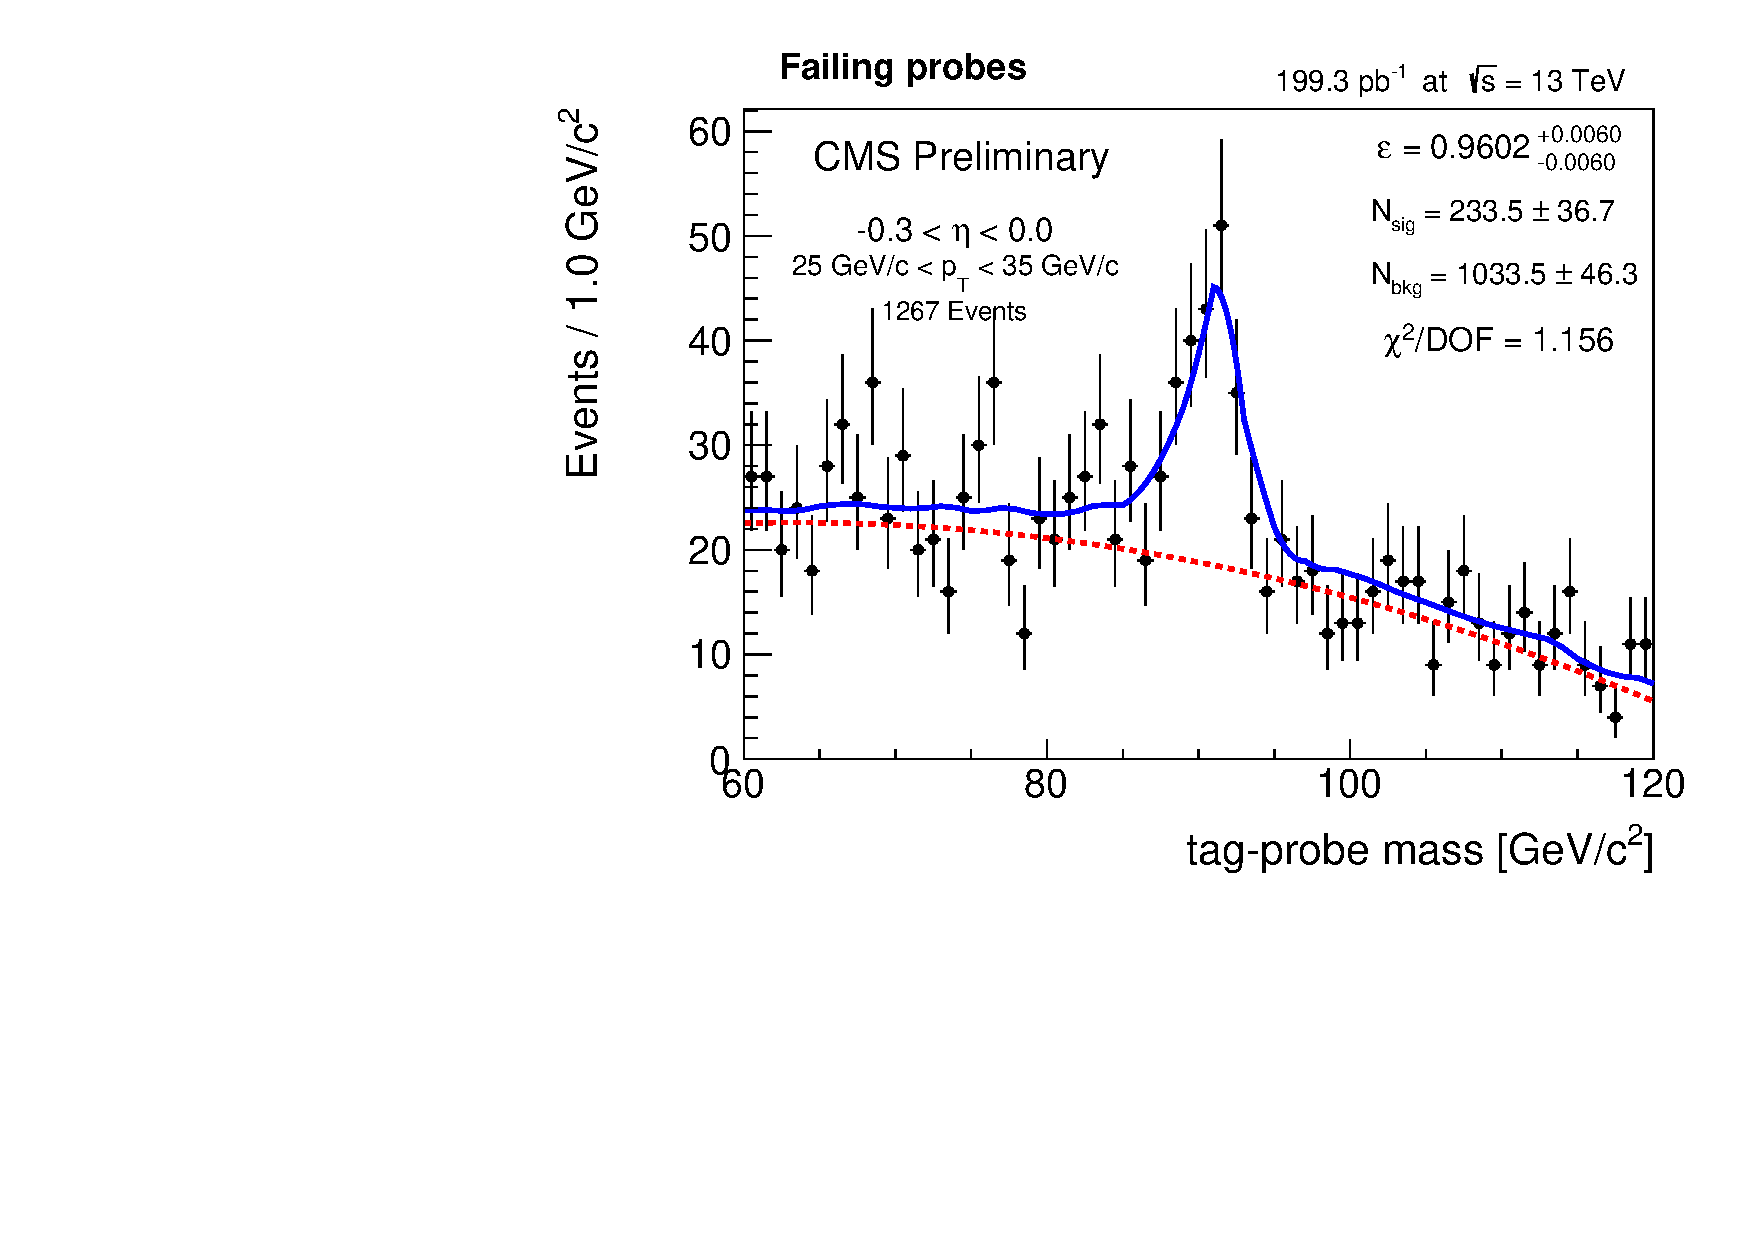
\includegraphics[width=.49\linewidth]{plots/efficiency/examples_musta/failetapt_5.pdf}
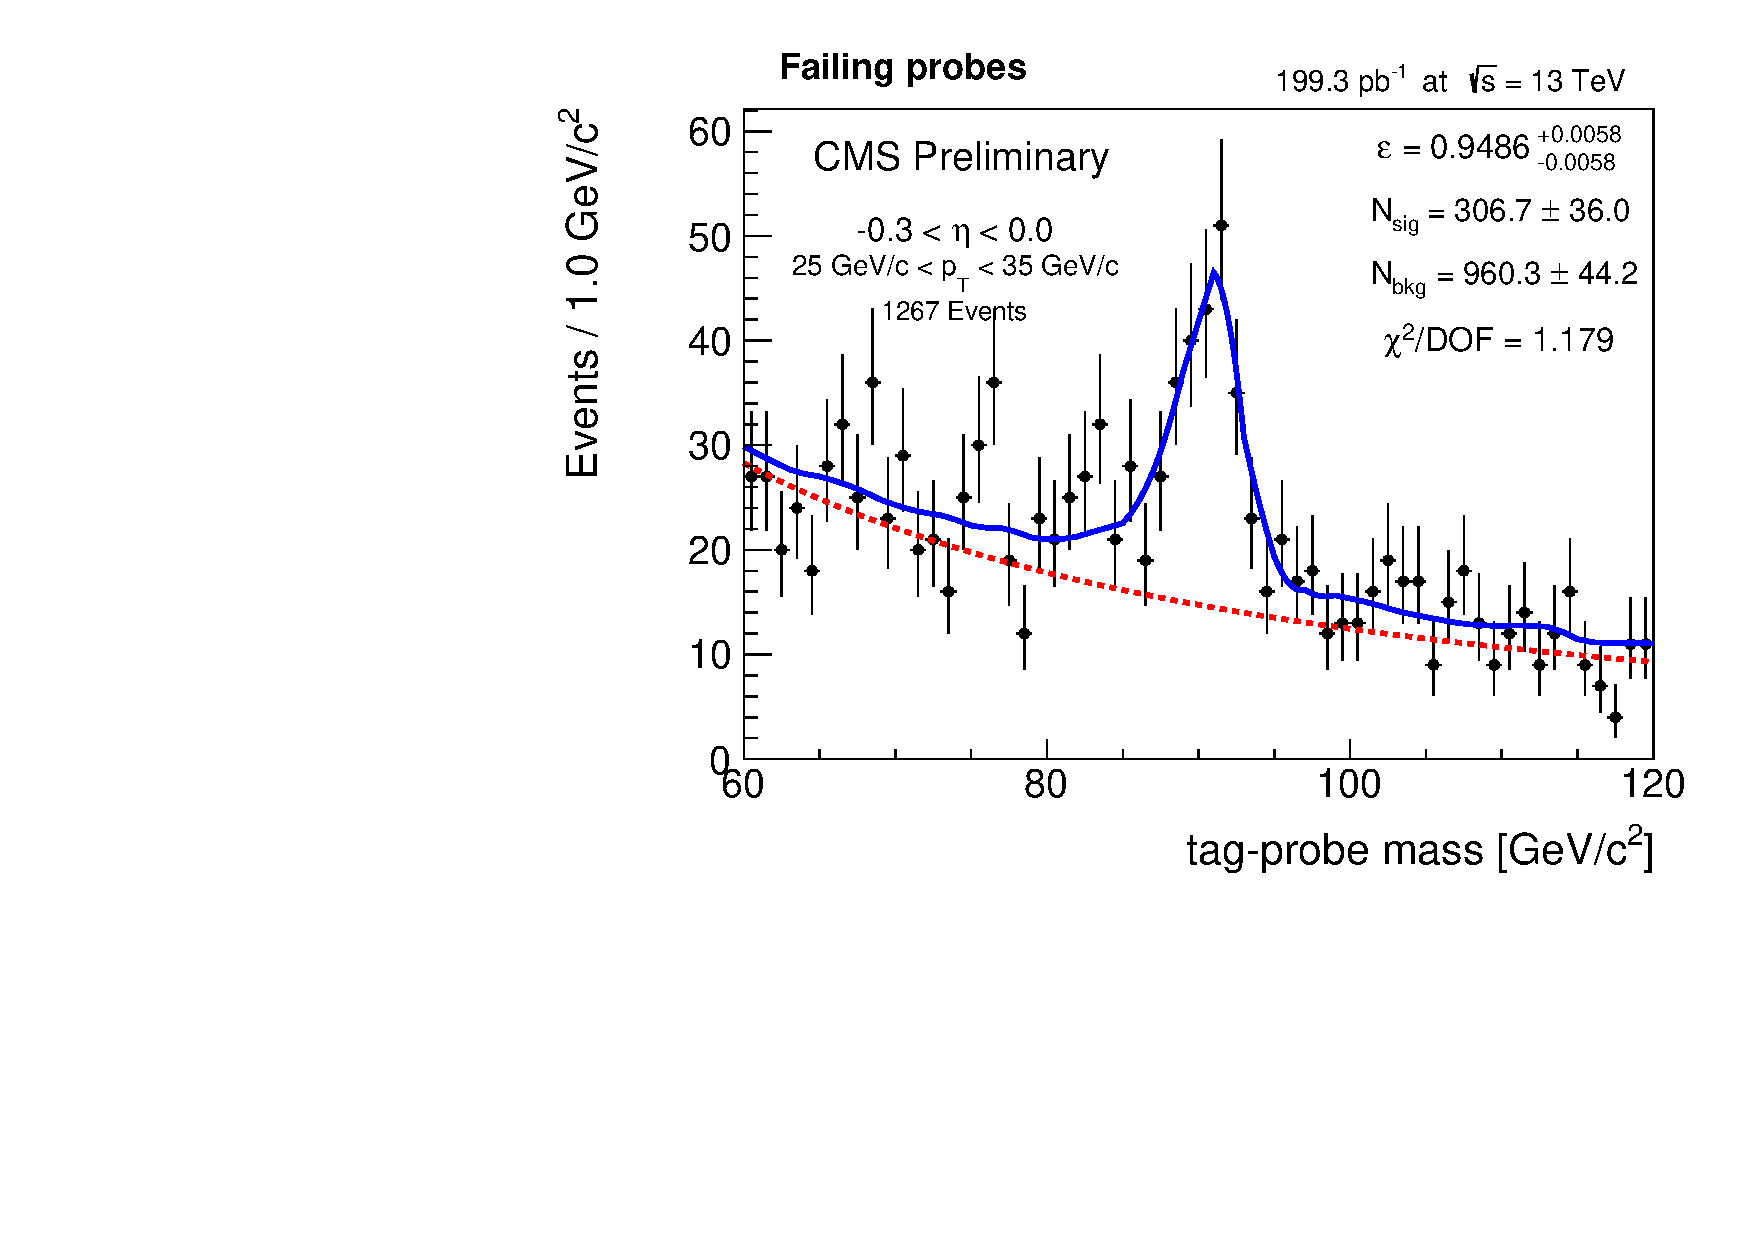
\includegraphics[width=.49\linewidth]{plots/efficiency/examples_plbkg/failetapt_5.pdf}
\caption{Examples of passing (top) and failing (bottom) probes from the same $p_T-\eta$ bin, from the muon standalone efficiency, fit with two different background models. The left plots use a quadratic polynomial and the right plots use a power law (shown in red).}
\label{fig:eff:musta:fitexample}
\end{figure}


\subsubsection{Tag Selection Uncertainty}
Uncertainty due to the selection criteria of the tag lepton are evaluated by directly comparing the impact of efficiency scale factors using the standard cut ($\pt > 25 \GeV$) to efficiency scale factors derived using tag leptons with $\pt > 30\GeV$. 

% \subsection{Summary of Systematic Uncertainties}
% A summary of the systematic uncertainties on the efficiency scale factors can be found in the Systematics Chapter later. 
% The impact of alternate models is evaluated by propagating the difference between models as a modification to the efficiency scale factor, and computing the selection-level acceptance with each of the alternative efficiency models. 
% Contributions of each type of systematic uncertainty are listed in the Tables ~\ref{tab:Eff:Unc:muon:summary:13} and ~\ref{tab:Eff:Unc:ele:summary:13} for 13 TeV and Table~\ref{tab:Eff:Unc:ele:summary:5} and Table~\ref{tab:Eff:Unc:mu:summary:5} for 5 TeV. 

\subsection{Statistical Uncertainty}
Statistical uncertainties in the efficiency scale factor are taken from the average over all variations on the measurement. The statistical uncertainty for a single $(\pt,\eta)$ bin is treated as Poisson, as given in Ref.~\cite{Paterno:2004cb}. Uncertainties for a given $(\pt,\eta)$ bin are correlated across all events containing leptons in the bin, while the uncertainties from separate $(\pt,\eta)$ bins are treated as uncorrelated. Individual categories (reconstruction, identification and isolation, trigger, etc.) are also treated as uncorrelated. The overall impact on the signal yield from the efficiency scale factor statistical uncertainties for the electron and muon channels in \serag and \serah are listed in Table~\ref{tab:eff:stat:all}.
%%%% Table containing the $e$ ID+Iso cuts
\begin{table}%[htbp]
\begin{center}

\scalebox{1.0}{
\begin{tabular}{|c|c|c|}
\hline
(13 TeV) & electron [\%] & muon [\%]\\
\hline \hline
$W^+$     & 0.489 & 0.291 \\
$W^-$     & 0.485 & 0.278 \\
$Z$       & 0.498 & 0.283 \\
\hline
\end{tabular} }
\quad
\scalebox{1.0}{
\begin{tabular}{|c|c|c|}
\hline
(5 TeV) & electron [\%] & muon [\%]\\
\hline \hline
$W^+$     & 0.489 & 0.245 \\
$W^-$     & 0.471 & 0.231\\
$Z$       & 0.526 & 0.268 \\
\hline
\end{tabular} }

\end{center}

\caption{Statistical uncertainty [\%] in the efficiency scale factor calculations on the \Wp, \Wm, and \Z boson acceptance at \sh (left) and \sg (right).}
\label{tab:eff:stat:all}
\end{table}

% \begin{table}[htbp]
\begin{center}
\begin{tabular}{ccccccccc}
\hline
Source & $W^+$& $W^-$ & $W$ & $W^+/W^-$ & $Z$ & $W^+/Z$&$W^+/Z$ &$W/Z$  \\
\hline \hline
FSR & 0.191 & 0.169 & 0.181 & 0.021 & 0.238 & 0.049 & 0.070 & 0.058 \\
MC & 0.073 & 0.067 & 0.070 & 0.006 & 0.094 & 0.023 & 0.029 & 0.025 \\
Background & 0.007 & 0.008 & 0.008 & 0.000 & 0.012 & 0.002 & 0.002 & 0.002 \\
Tag pT & 0.033 & 0.038 & 0.035 & 0.004 & 0.093 & 0.058 & 0.054 & 0.056 \\
Statistical & 0.286 & 0.278 & 0.202 & 0.009 & 0.279 & 0.008 & 0.001 & 0.076 \\
\hline \hline
Total [\%] & 0.35 & 0.33 & 0.28 & 0.00 & 0.39 & 0.07 & 0.08 & 0.10 \\

\end{tabular}
\end{center}
\caption{Uncertainties on the lepton efficiency scale factors for the muon channel in 13 TeV}
\label{tab:Eff:Unc:muon:summary:13}
\end{table}

% \begin{table}[htbp]
\begin{center}
\begin{tabular}{ccccccccc}
\hline
Source & $W^+$& $W^-$ & $W$ & $W^+/W^-$ & $Z$ & $W^+/Z$&$W^+/Z$ &$W/Z$  \\
\hline \hline
FSR & 0.081 & 0.080 & 0.081 & 0.001 & 0.166 & 0.087 & 0.089 & 0.085 \\
MC & 0.057 & 0.057 & 0.056 & 0.000 & 0.093 & 0.038 & 0.038 & 0.036 \\
Background & 0.056 & 0.053 & 0.055 & 0.004 & 0.099 & 0.041 & 0.044 & 0.045 \\
Tag pT & 0.016 & 0.018 & 0.017 & 0.001 & 0.047 & 0.066 & 0.067 & 0.063 \\
Statistical & 0.489 & 0.486 & 0.349 & 0.001 & 0.488 & 0.002 & 0.003 & 0.137 \\
\hline \hline
Total [\%] & 0.50 & 0.50 & 0.36 & 0.00 & 0.53 & 0.11 & 0.11 & 0.18 \\


\end{tabular}
\end{center}
\caption{Uncertainties on the lepton efficiency scale factors for the electron channel in 13 TeV}
\label{tab:Eff:Unc:ele:summary:13}
\end{table}
% %%%% Summary of lep eff systematics for muons - 5 TeV  %%%%%
\begin{table}[htbp]
\begin{center}
\begin{tabular}{ccccccccc}
\hline
Source & $W^+$& $W^-$ & $W$ & $W^+/W^-$ & $Z$ & $W^+/Z$&$W^+/Z$ &$W/Z$  \\
\hline \hline
MC & 0.09 & 0.08 & 0.09 & 0.00 & 0.15 & 0.07 & 0.07 & 0.07 \\
FSR & 0.17 & 0.15 & 0.32 & 0.01 & 0.27 & 0.23 & 0.26 & 0.24 \\
Bkg Model & 0.01 & 0.01 & 0.01 & 0.01 & 0.00 & 0.01 & 0.01 & 0.01 \\
Tag pT & 0.48 & 0.49 & 0.48 & 0.01 & 0.88 & 0.45 & 0.45 & 0.45 \\
stat & 0.25 & 0.24 & 0.20 & 0.32 & 0.26 & 0.38 & 0.36 & 0.35 \\
 \\
\hline \hline
Total [\%] & 0.56 & 0.56 & 0.61 & 0.32 & 0.96 & 0.62 & 0.62 & 0.61 \\
\end{tabular}
\end{center}
\caption{Summary of the propagated muon efficiency systematic uncertainties at 5 TeV.}
\label{tab:Eff:Unc:mu:summary:5}
\end{table}

% %%%% Summary of lep eff systematics for electrons - 5 TeV  %%%%%
\begin{table}%[htbp]
\begin{center}
\scalebox{0.7}{
\begin{tabular}{ccccccccc}
\hline
Source & $W^+$& $W^-$ & $W$ & $W^+/W^-$ & $Z$ & $W^+/Z$&$W^+/Z$ &$W/Z$  \\
\hline \hline
Binning [\%] & 0.00  & 0.00 & 0.00 & 0.00 & 0.00& 0.00& 0.00& 0.00\\
Signal Shape [\%] & 0.00  & 0.00 & 0.00 & 0.00 & 0.00& 0.00& 0.00& 0.00 \\
Background Shape [\%] & 0.00  & 0.00 & 0.00 & 0.00 & 0.00& 0.00& 0.00& 0.00  \\
\hline
\end{tabular}}
\end{center}
\caption{Summary of the propagated electron efficiency systematic uncertainties at 5 TeV.}
\label{tab:Eff:Unc:ele:summary:5}
\end{table}

% %%%% Summary of lep eff systematics for electrons - 13/5 TeV ratios  %%%%%
\begin{table}%[htbp]
\begin{center}
\scalebox{0.7}{
\begin{tabular}{ccccccccc}
\hline
Source & $W^+$& $W^-$ & $W$ & $W^+/W^-$ & $Z$ & $W^+/Z$&$W^+/Z$ &$W/Z$ \\
\hline \hline
Binning [\%] & 0.00  & 0.00 & 0.00 & 0.00 & 0.00& 0.00& 0.00& 0.00 \\
Signal Shape [\%] & 0.00  & 0.00 & 0.00 & 0.00 & 0.00& 0.00& 0.00& 0.00 \\
Background Shape [\%] & 0.00  & 0.00 & 0.00 & 0.00 & 0.00& 0.00& 0.00& 0.00  \\
\hline
\end{tabular}}
\end{center}
\caption{Summary of the propagated electron efficiency systematic uncertainties for the 13TeV/5TeV ratio.}
\label{tab:Eff:Unc:ele:summary:13to5}
\end{table}

% %%%% Summary of lep eff systematics for muons - 13/5 TeV ratios  %%%%%
\begin{table}%[htbp]
\begin{center}
\scalebox{0.7}{
\begin{tabular}{ccccccccc}
\hline
Source & $W^+$& $W^-$ & $W$ & $W^+/W^-$ & $Z$ & $W^+/Z$&$W^+/Z$ &$W/Z$  \\
\hline \hline
Binning [\%]          & 0.00  & 0.00 & 0.00 & 0.00 & 0.00& 0.00& 0.00 & 0.00 \\
Signal Shape [\%]     & 0.00  & 0.00 & 0.00 & 0.00 & 0.00& 0.00& 0.00 & 0.00 \\
Background Shape [\%] & 0.00  & 0.00 & 0.00 & 0.00 & 0.00& 0.00& 0.00 & 0.00  \\
\hline
\end{tabular}
}
\end{center}
\caption{Summary of the propagated muon efficiency systematic uncertainties for the 13 Tev/5 TeV ratio.}
\label{tab:Eff:Unc:mu:summary:13to5}
\end{table}




%% %%%%%%%%%%%%%%%%%%%%%%%%%%%
%%                Results
%%%%%%%%%%%%%%%%%%%%%%%%%%%%%
\section{Results}\label{ch:eff:results}
Distributions of $\eta$ dependence of efficiencies in data and simulation by $\pt$ bins for all lepton categories are provided, as well as tables containing total scale factors and statistical uncertainties. A list of tables and figures for \serag in Table~\ref{tab:eff:list:5} and for \serah is provided in Table~\ref{tab:eff:list:13}.
\begin{table}[htbp]
\begin{center}
\scalebox{1.0}{
\begin{tabular}{lcc}
\hline
Category [13 TeV] & Figure & Table   \\
\hline \hline
electron GSF+ID+Iso &  \ref{fig:Eff:el:13:GSFSel:com} &  \ref{tab:Eff:el:13TeV:GSFSel:com} \\
electron trigger & \ref{fig:Eff:el:13:HLT:pos}$(+)$,~ \ref{fig:Eff:el:13:HLT:neg}$(-)$ & \ref{tab:Eff:el:13TeV:HLT:pos}$(+)$,~\ref{tab:Eff:el:13TeV:HLT:neg}$(-)$ \\
muon Sel.+ID+Iso & \ref{fig:Eff:mu:13:SIT:com} & \ref{tab:Eff:mu:13TeV:SIT:com} \\
muon standalone & \ref{fig:Eff:mu:13:Sta:com}  & \ref{tab:Eff:mu:13TeV:Sta:com} \\
muon trigger &\ref{fig:Eff:mu:13:HLT:pos}$(+)$,~\ref{fig:Eff:mu:13:HLT:neg}$(-)$ & \ref{tab:Eff:mu:13TeV:HLT:pos}$(+)$,~\ref{tab:Eff:mu:13TeV:HLT:neg}$(-)$ \\
\hline
Category [5 TeV] & Figure & Table   \\
\hline \hline
electron GSF+ID+Iso &  \ref{fig:Eff:el:5:GSFSel:com} &  \ref{tab:Eff:el:5TeV:GSFSel:com} \\
electron trigger & \ref{fig:Eff:el:5:HLT:pos}$(+)$,~ \ref{fig:Eff:el:5:HLT:neg}$(-)$ & \ref{tab:Eff:el:5TeV:HLT:pos}$(+)$,~\ref{tab:Eff:el:5TeV:HLT:neg}$(-)$ \\
muon Sel.+ID+Iso & \ref{fig:Eff:mu:5:SIT:com} & \ref{tab:Eff:mu:5TeV:SIT:com} \\
muon standalone & \ref{fig:Eff:mu:5:Sta:com}  & \ref{tab:Eff:mu:13TeV:Sta:com} \\
muon trigger &\ref{fig:Eff:mu:5:HLT:pos}$(+)$,~\ref{fig:Eff:mu:5:HLT:neg}$(-)$ & \ref{tab:Eff:mu:5TeV:HLT:pos}$(+)$,~\ref{tab:Eff:mu:5TeV:HLT:neg}$(-)$ \\
\hline
\end{tabular}}
\end{center}
\caption{List of tables and figures containing \serag and \serah lepton efficiency scale factors.}
\label{tab:eff:list}
\end{table}

% % 13 TeV electrons
%%%% Figures for EleGSFSel Efficiency  %%%%%
\begin{figure}
\centering
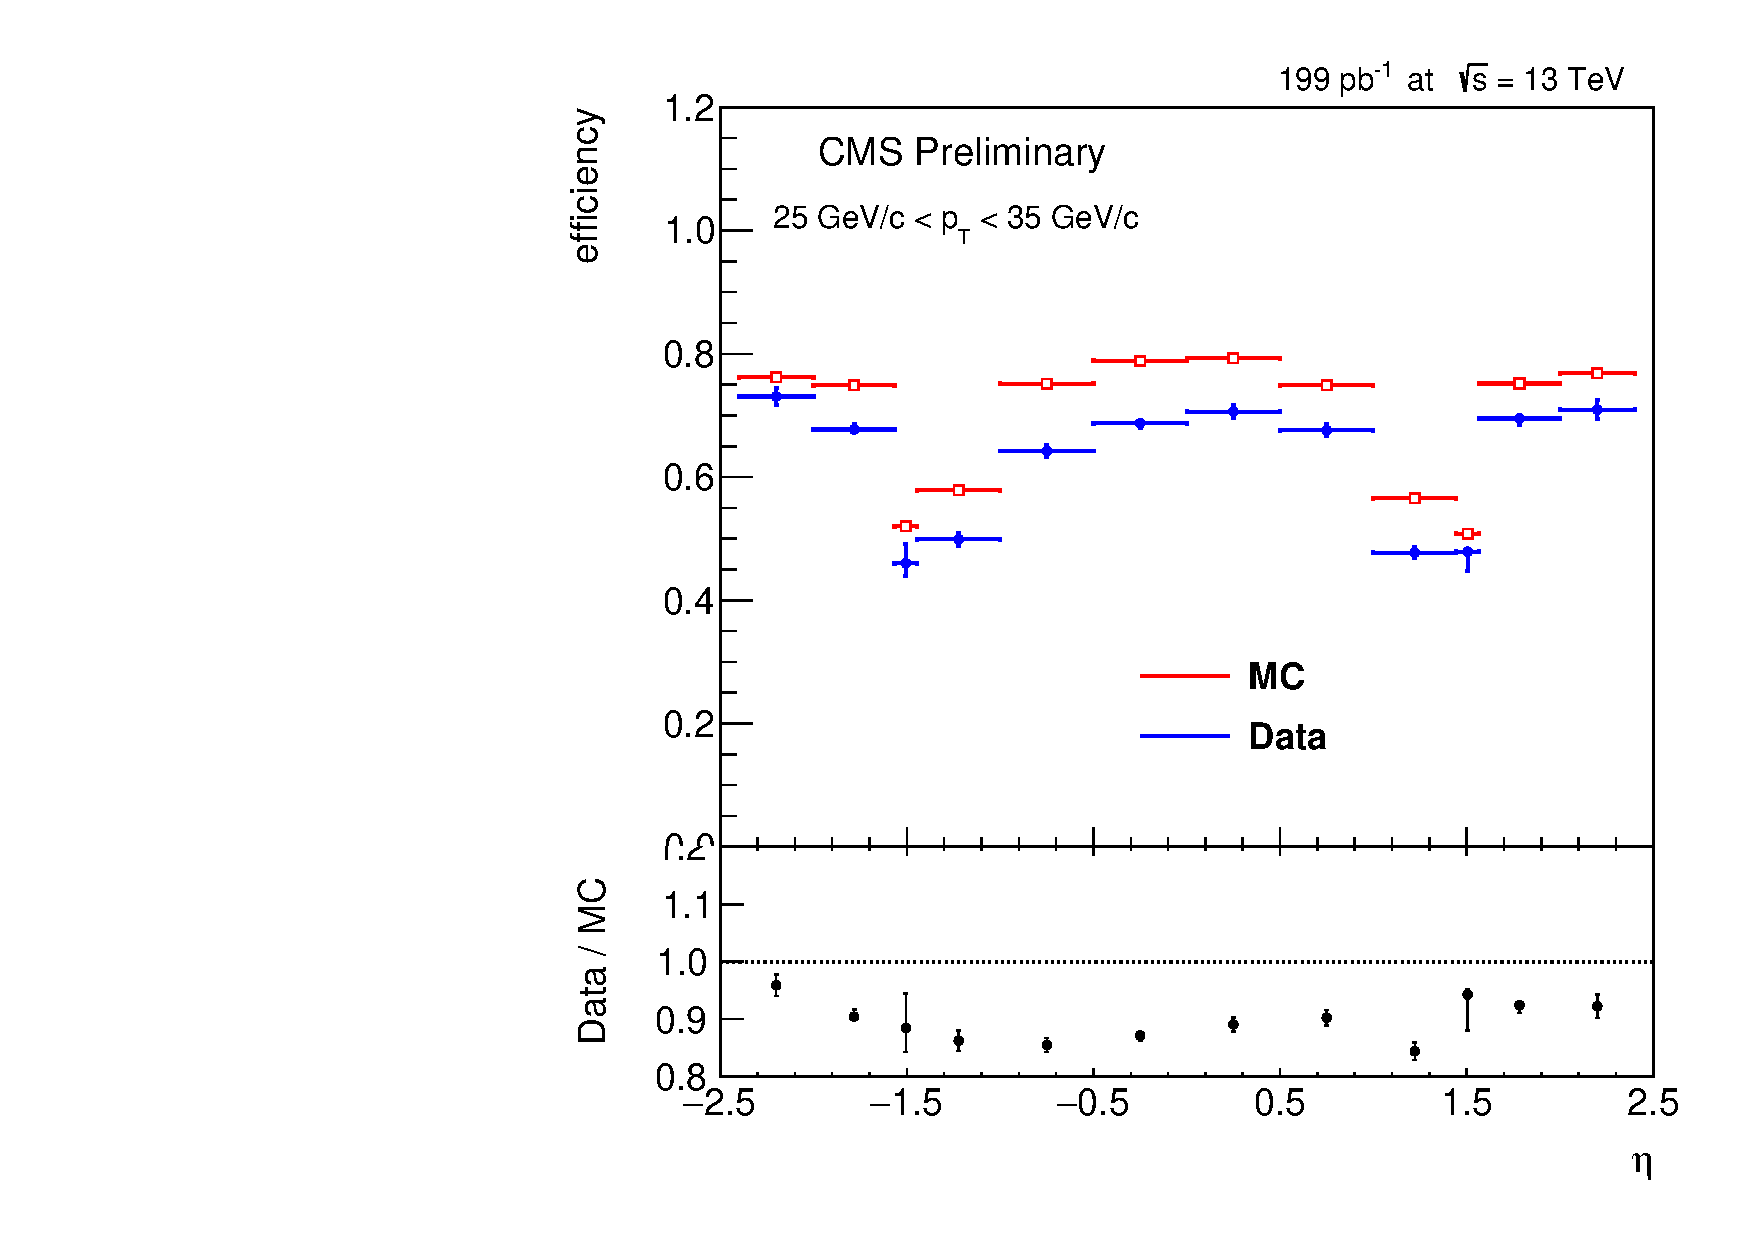
\includegraphics[width=0.48\linewidth]{plots/efficiency/13_zeegsfsel_combined/PtBins_eta_pt0.pdf}
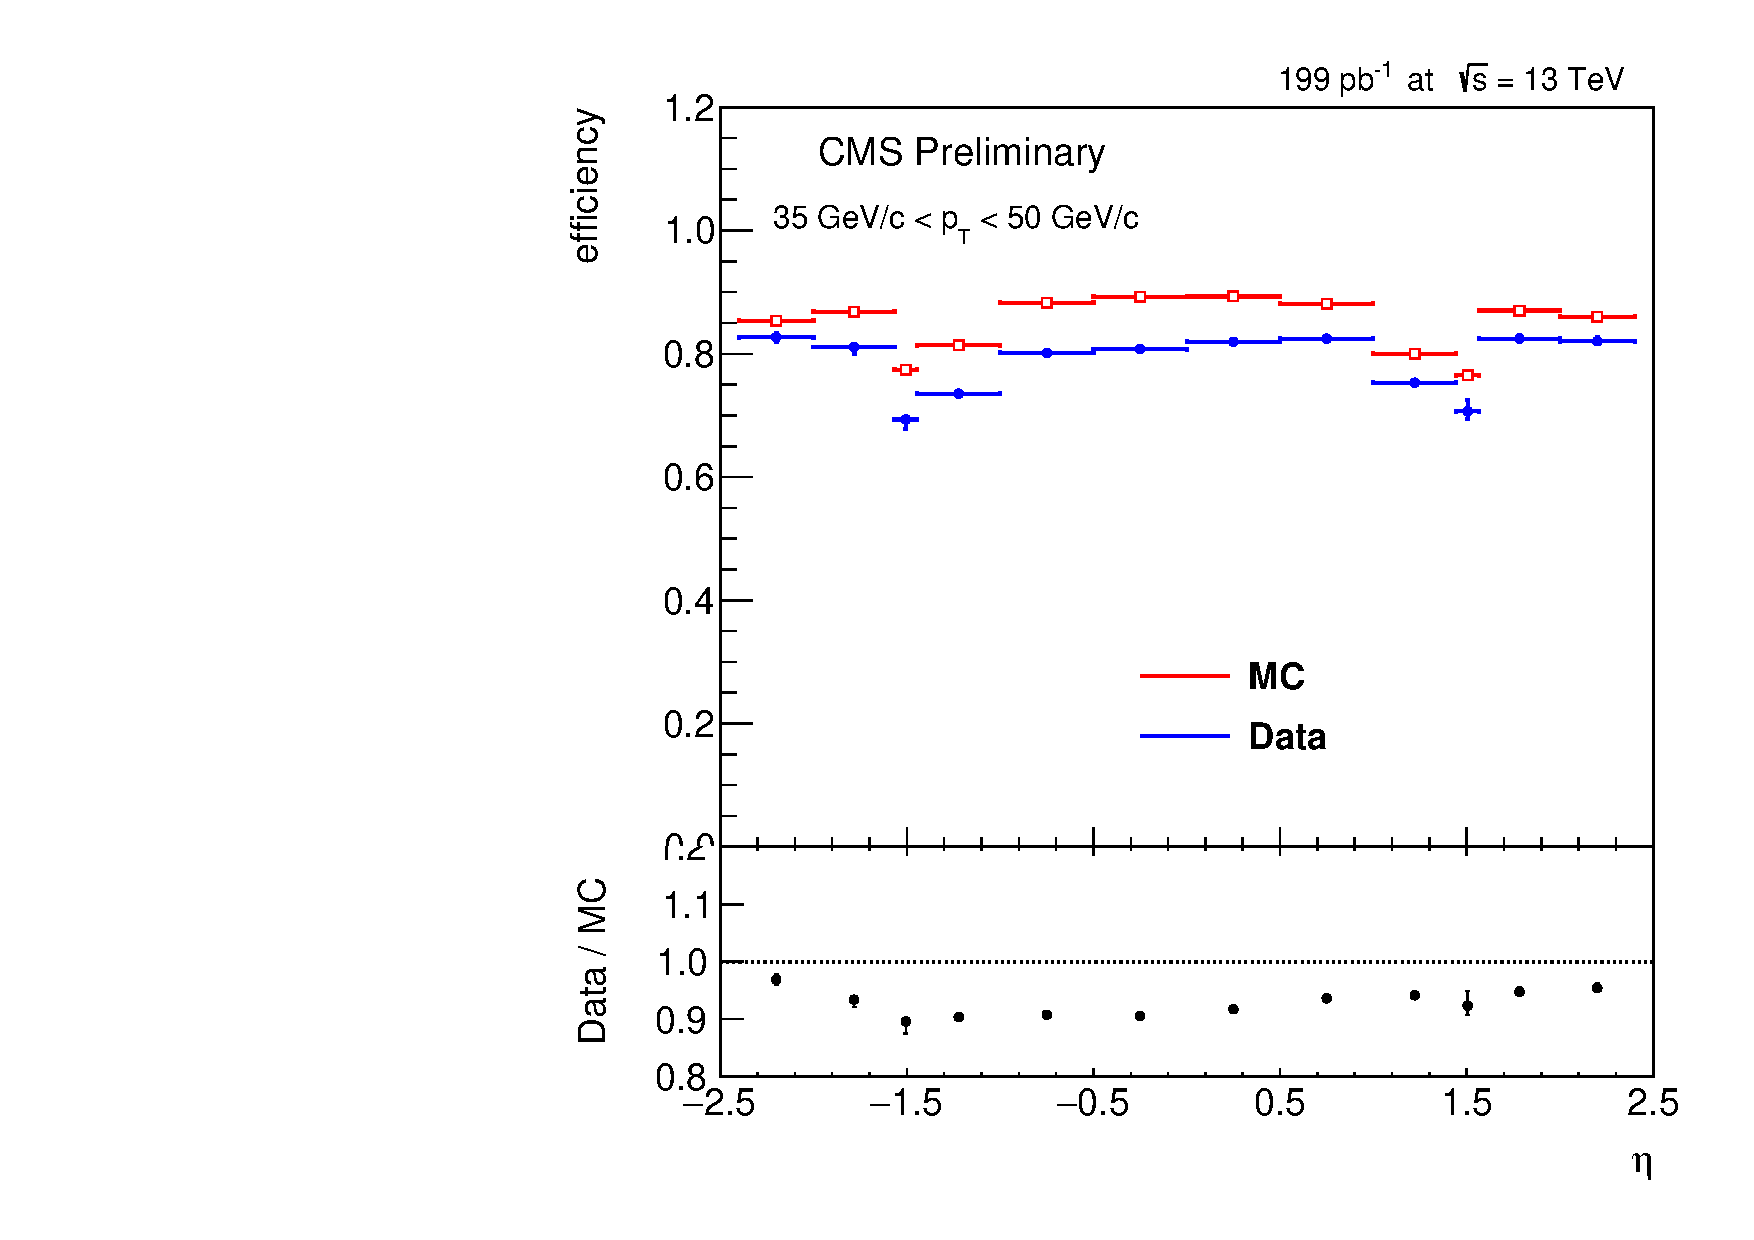
\includegraphics[width=0.48\linewidth]{plots/efficiency/13_zeegsfsel_combined/PtBins_eta_pt1.pdf}
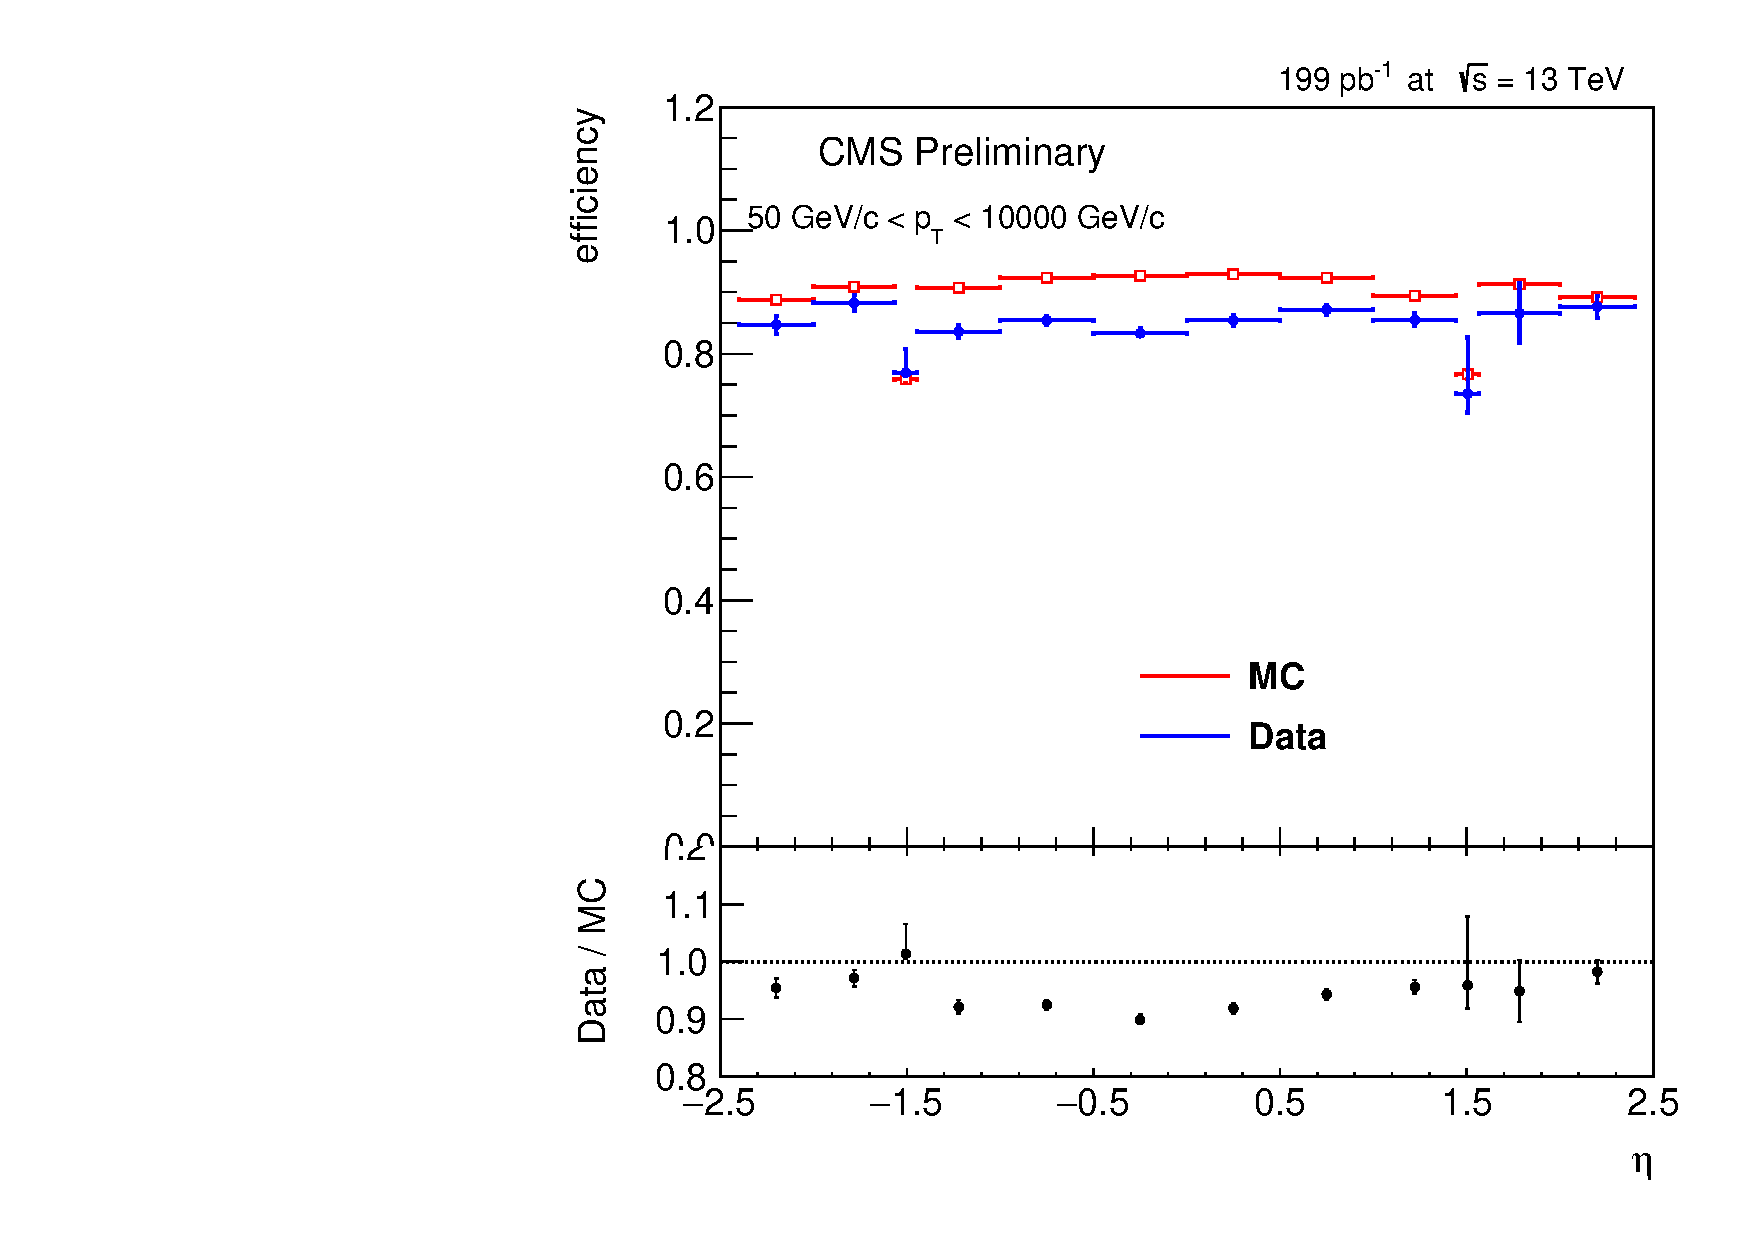
\includegraphics[width=0.48\linewidth]{plots/efficiency/13_zeegsfsel_combined/PtBins_eta_pt2.pdf}
\caption{$\eta$ dependence of GSF electron identification and isolation efficiency scale factors, separated by $p_T$ bins, for combined charged electrons in the 13 TeV samples.}
\label{fig:Eff:el:13:GSFSel:com}
\end{figure}

%%%% Figures for EleHLT Efficiency  %%%%%
\begin{figure}
\centering
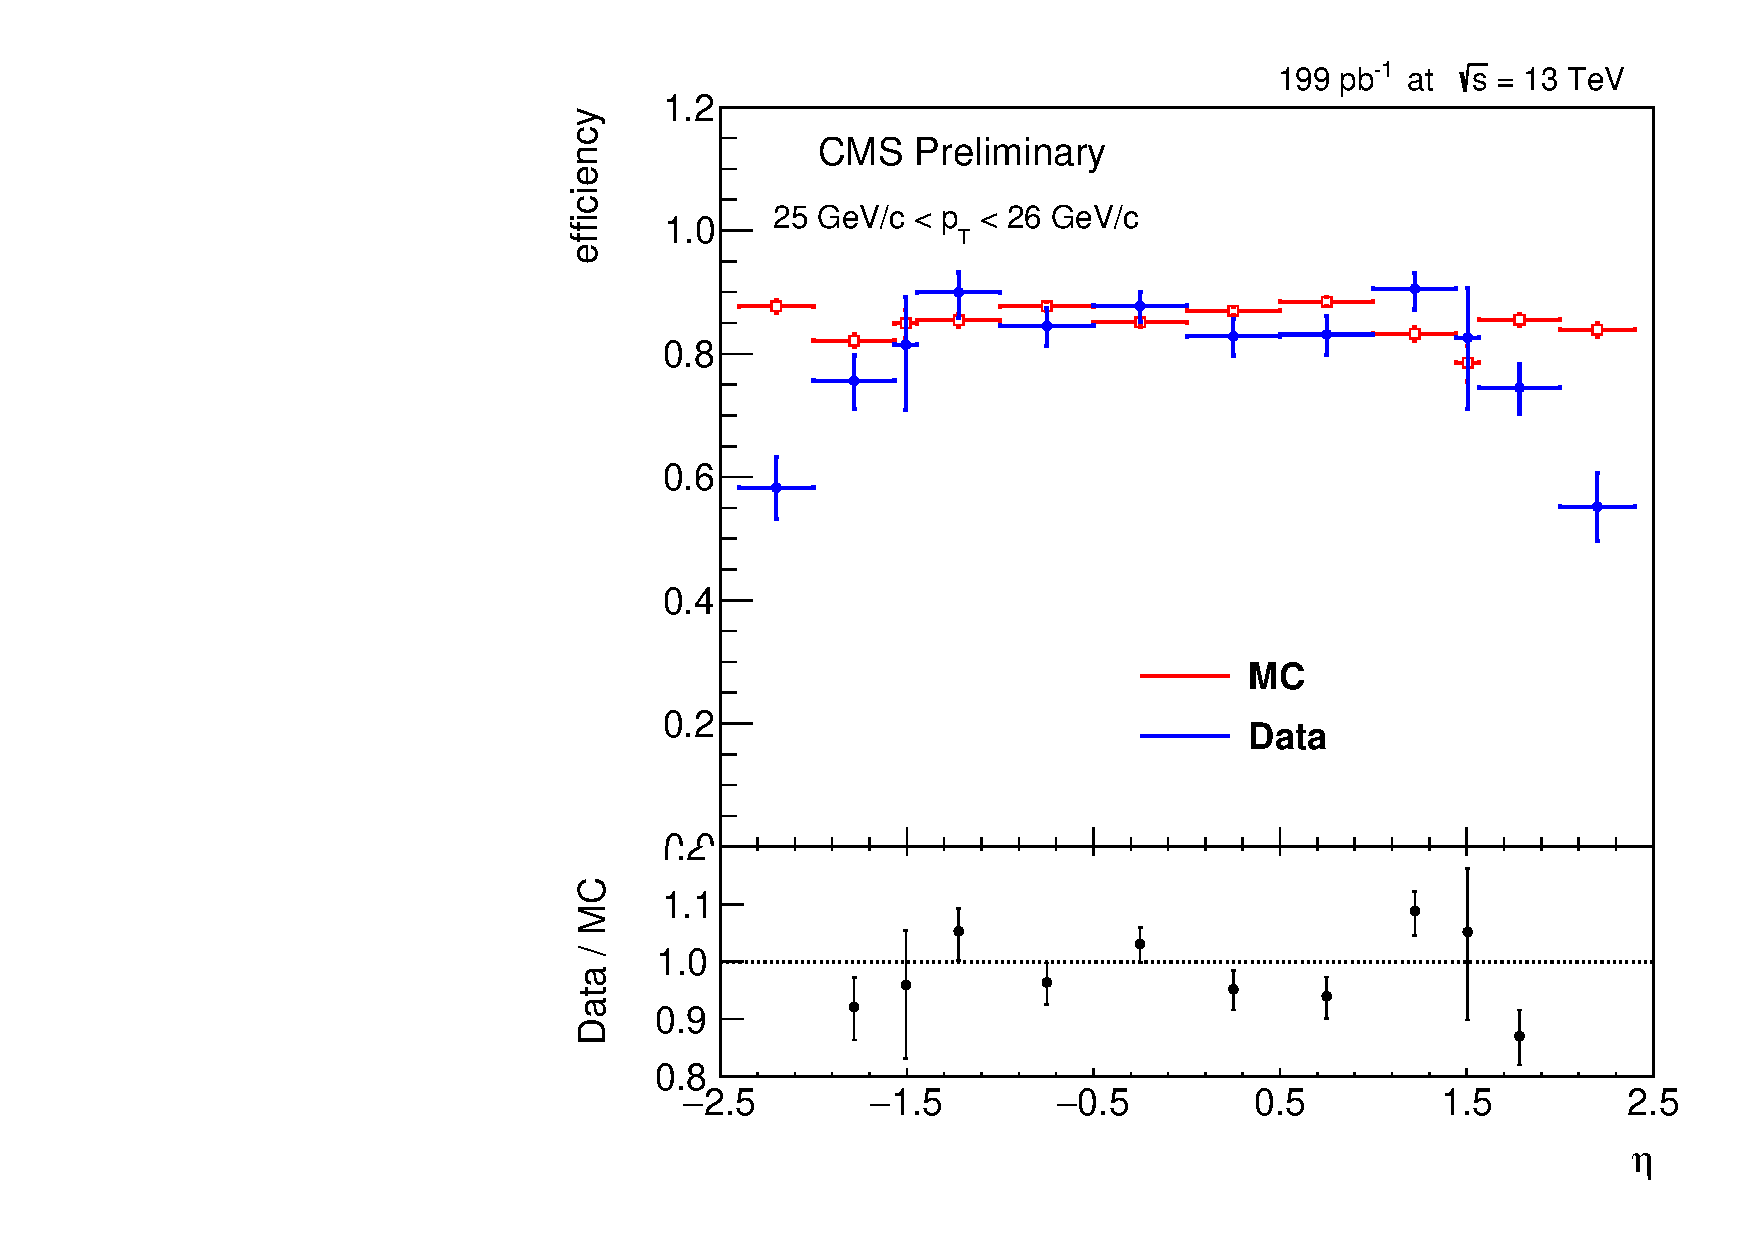
\includegraphics[width=0.45\linewidth]{plots/efficiency/13_zeehlt_positive/PtBins_eta_pt0.pdf}
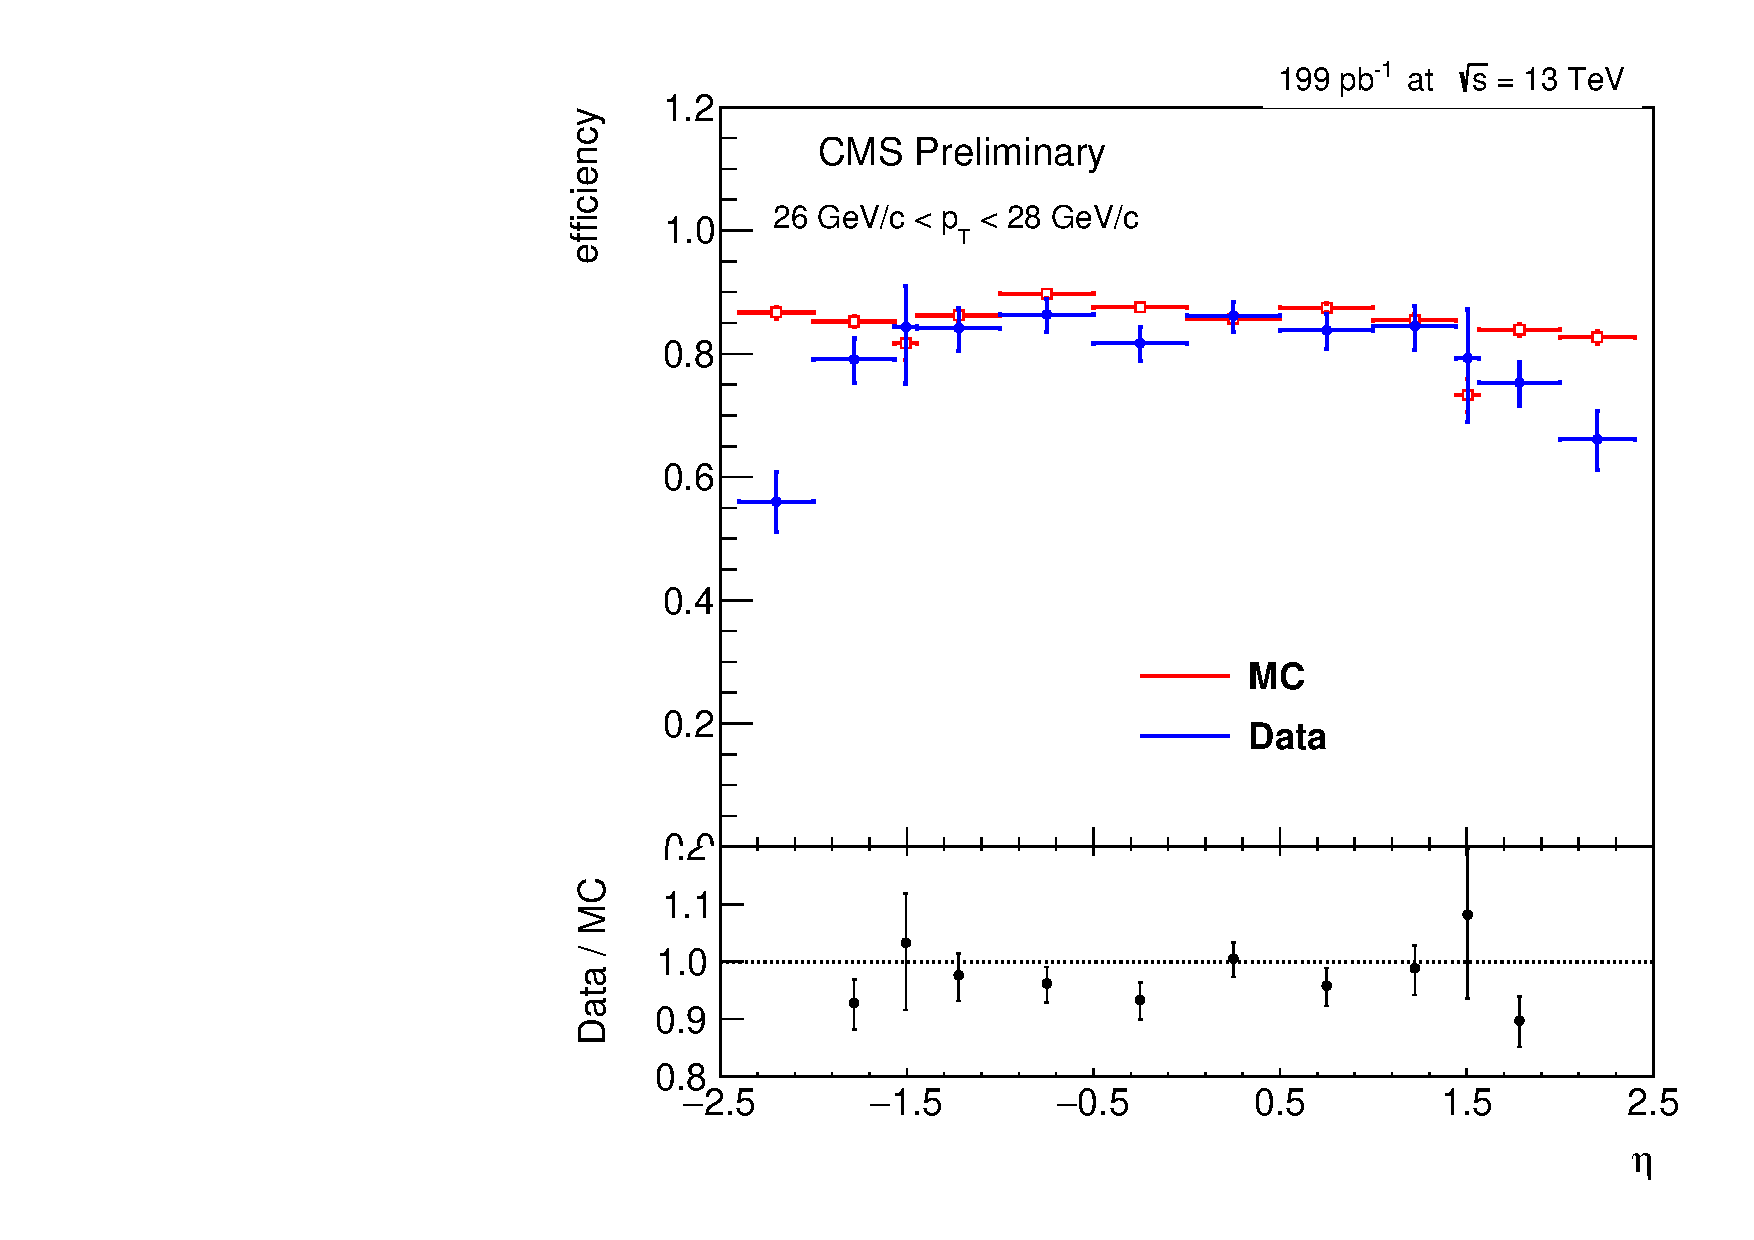
\includegraphics[width=0.45\linewidth]{plots/efficiency/13_zeehlt_positive/PtBins_eta_pt1.pdf}
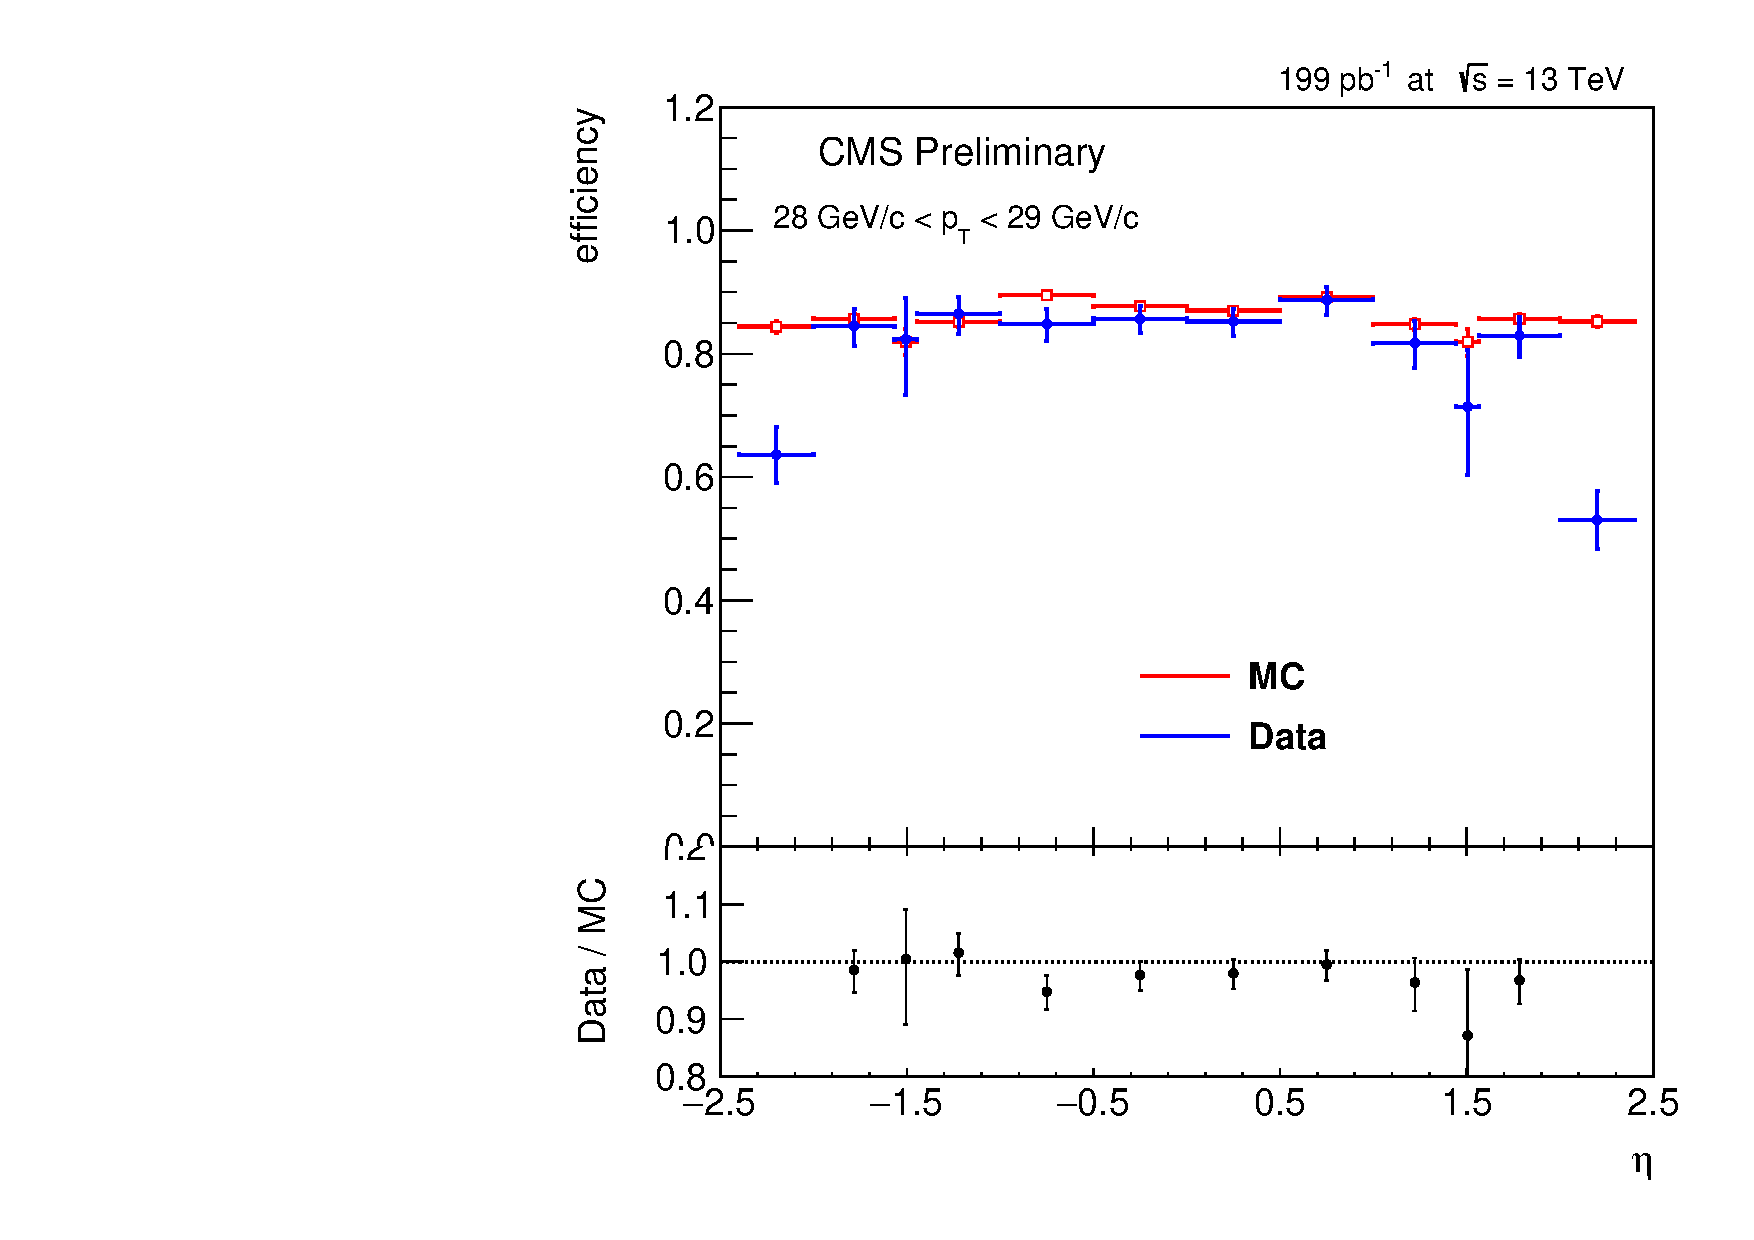
\includegraphics[width=0.45\linewidth]{plots/efficiency/13_zeehlt_positive/PtBins_eta_pt2.pdf}
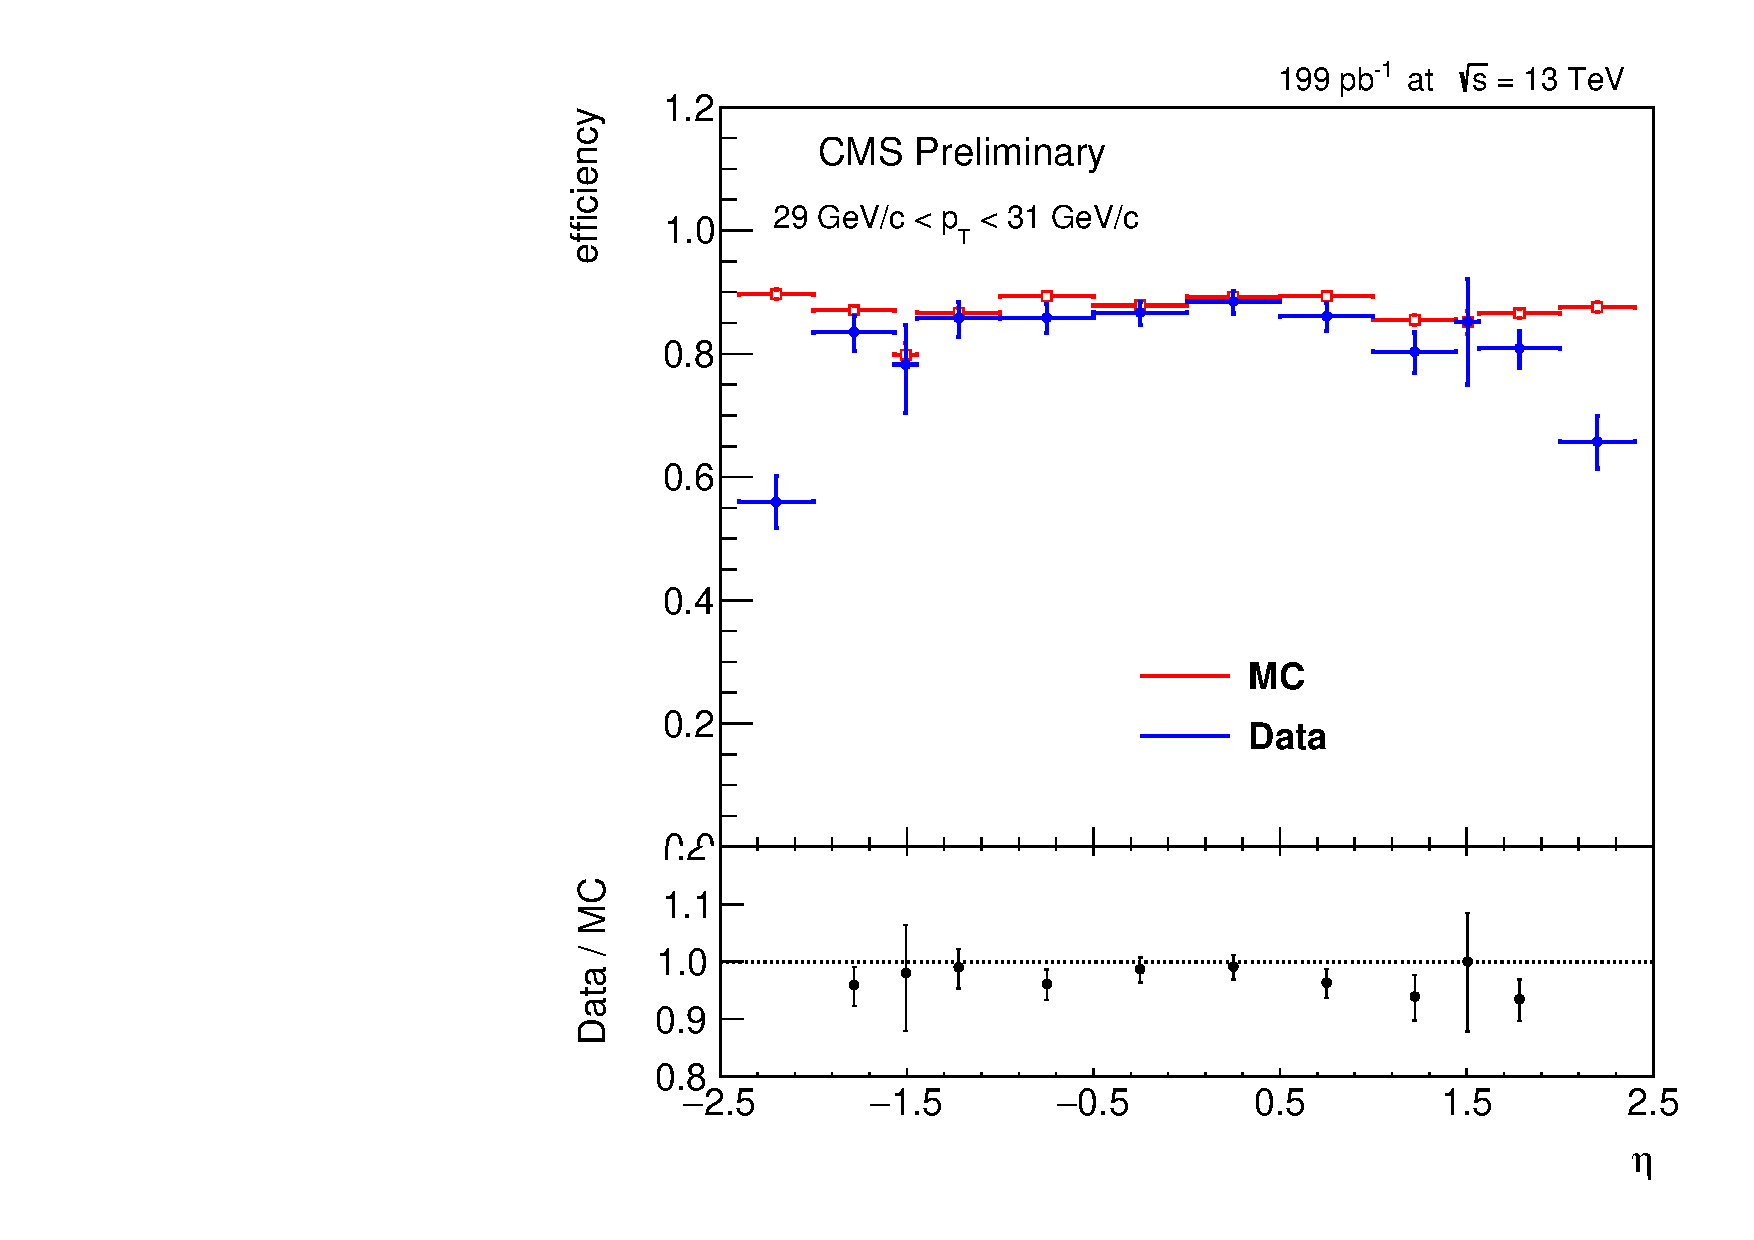
\includegraphics[width=0.45\linewidth]{plots/efficiency/13_zeehlt_positive/PtBins_eta_pt3.pdf}
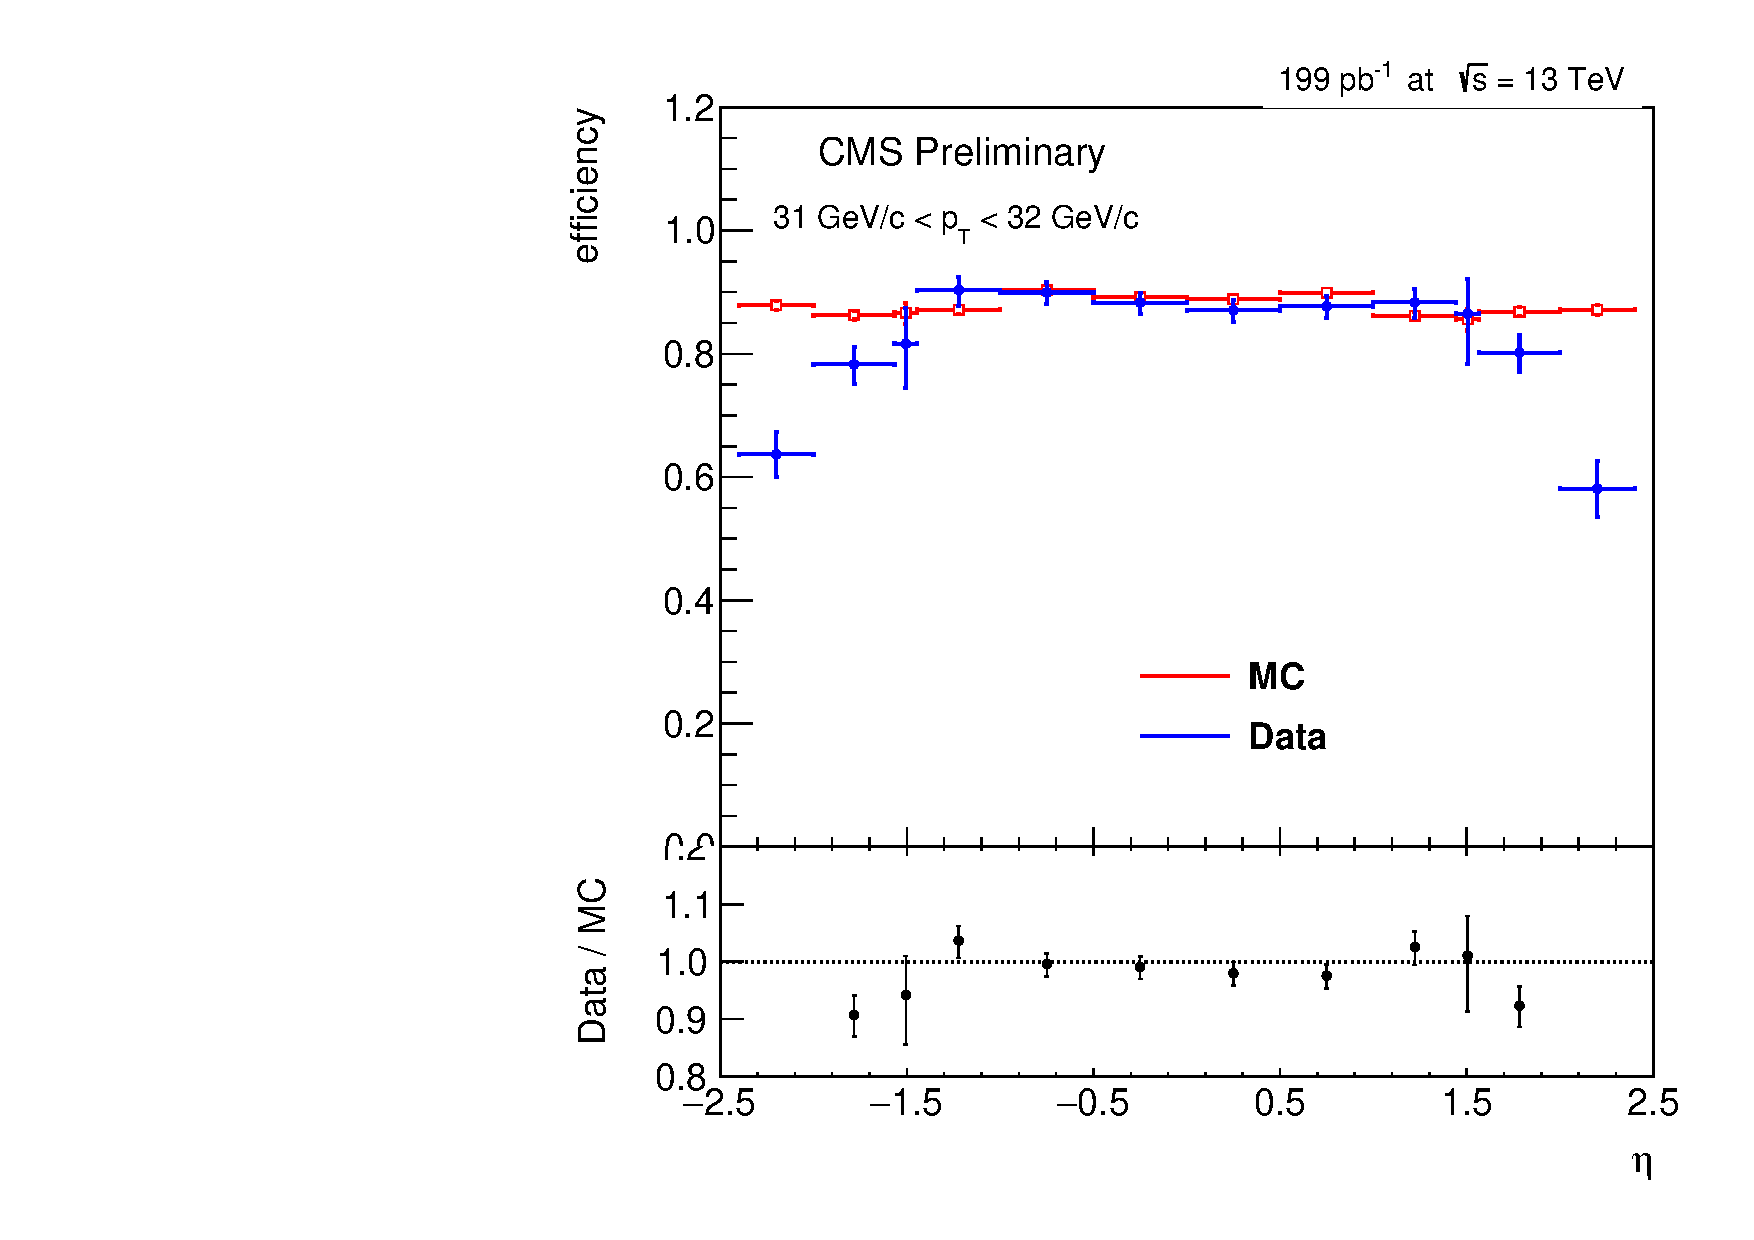
\includegraphics[width=0.45\linewidth]{plots/efficiency/13_zeehlt_positive/PtBins_eta_pt4.pdf}
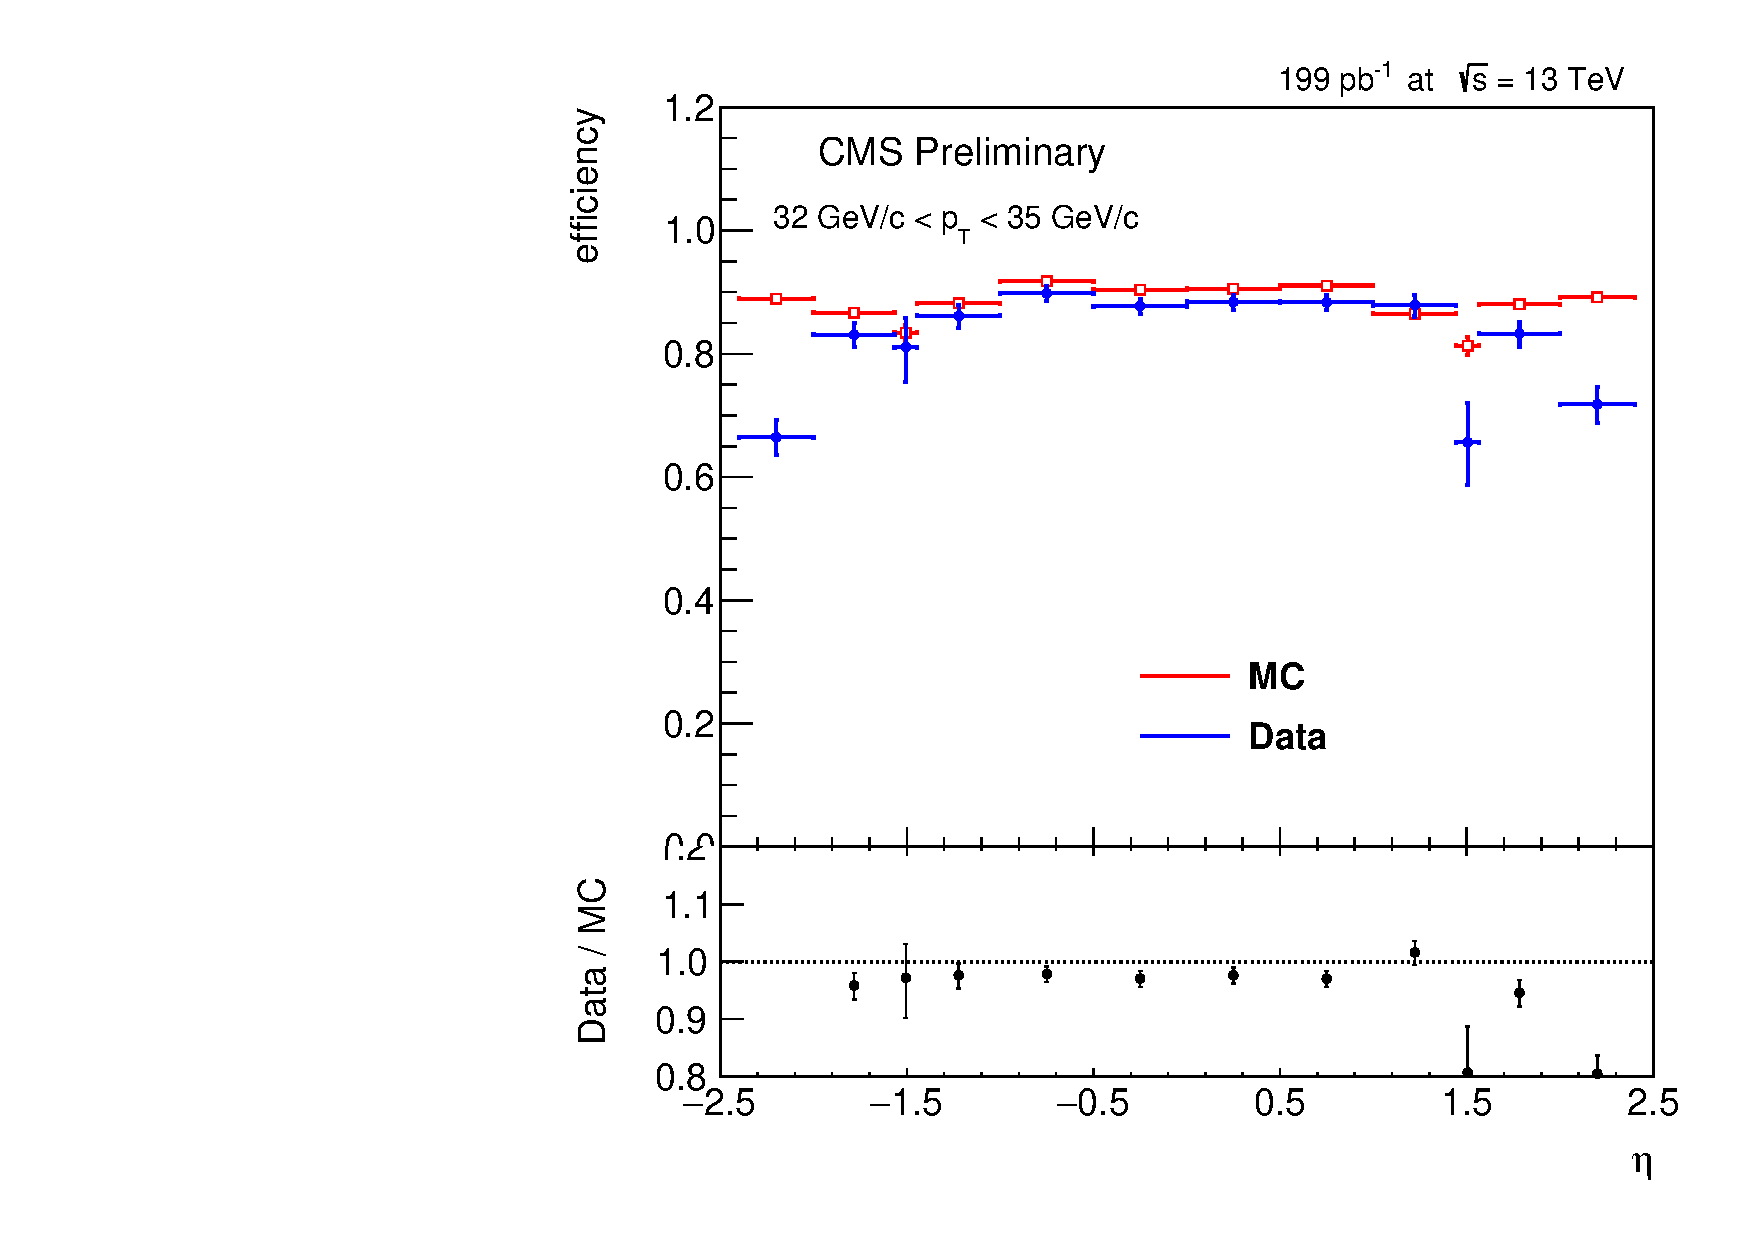
\includegraphics[width=0.45\linewidth]{plots/efficiency/13_zeehlt_positive/PtBins_eta_pt5.pdf}
\caption{$\eta$ dependence of Single electron trigger efficiency scale factors, separated by $p_T$ bins, for positively charged electrons in the 13 TeV samples.}
% \label{fig:Eff:el:13:HLT:pos}
\end{figure}
\begin{figure}
\ContinuedFloat
\centering
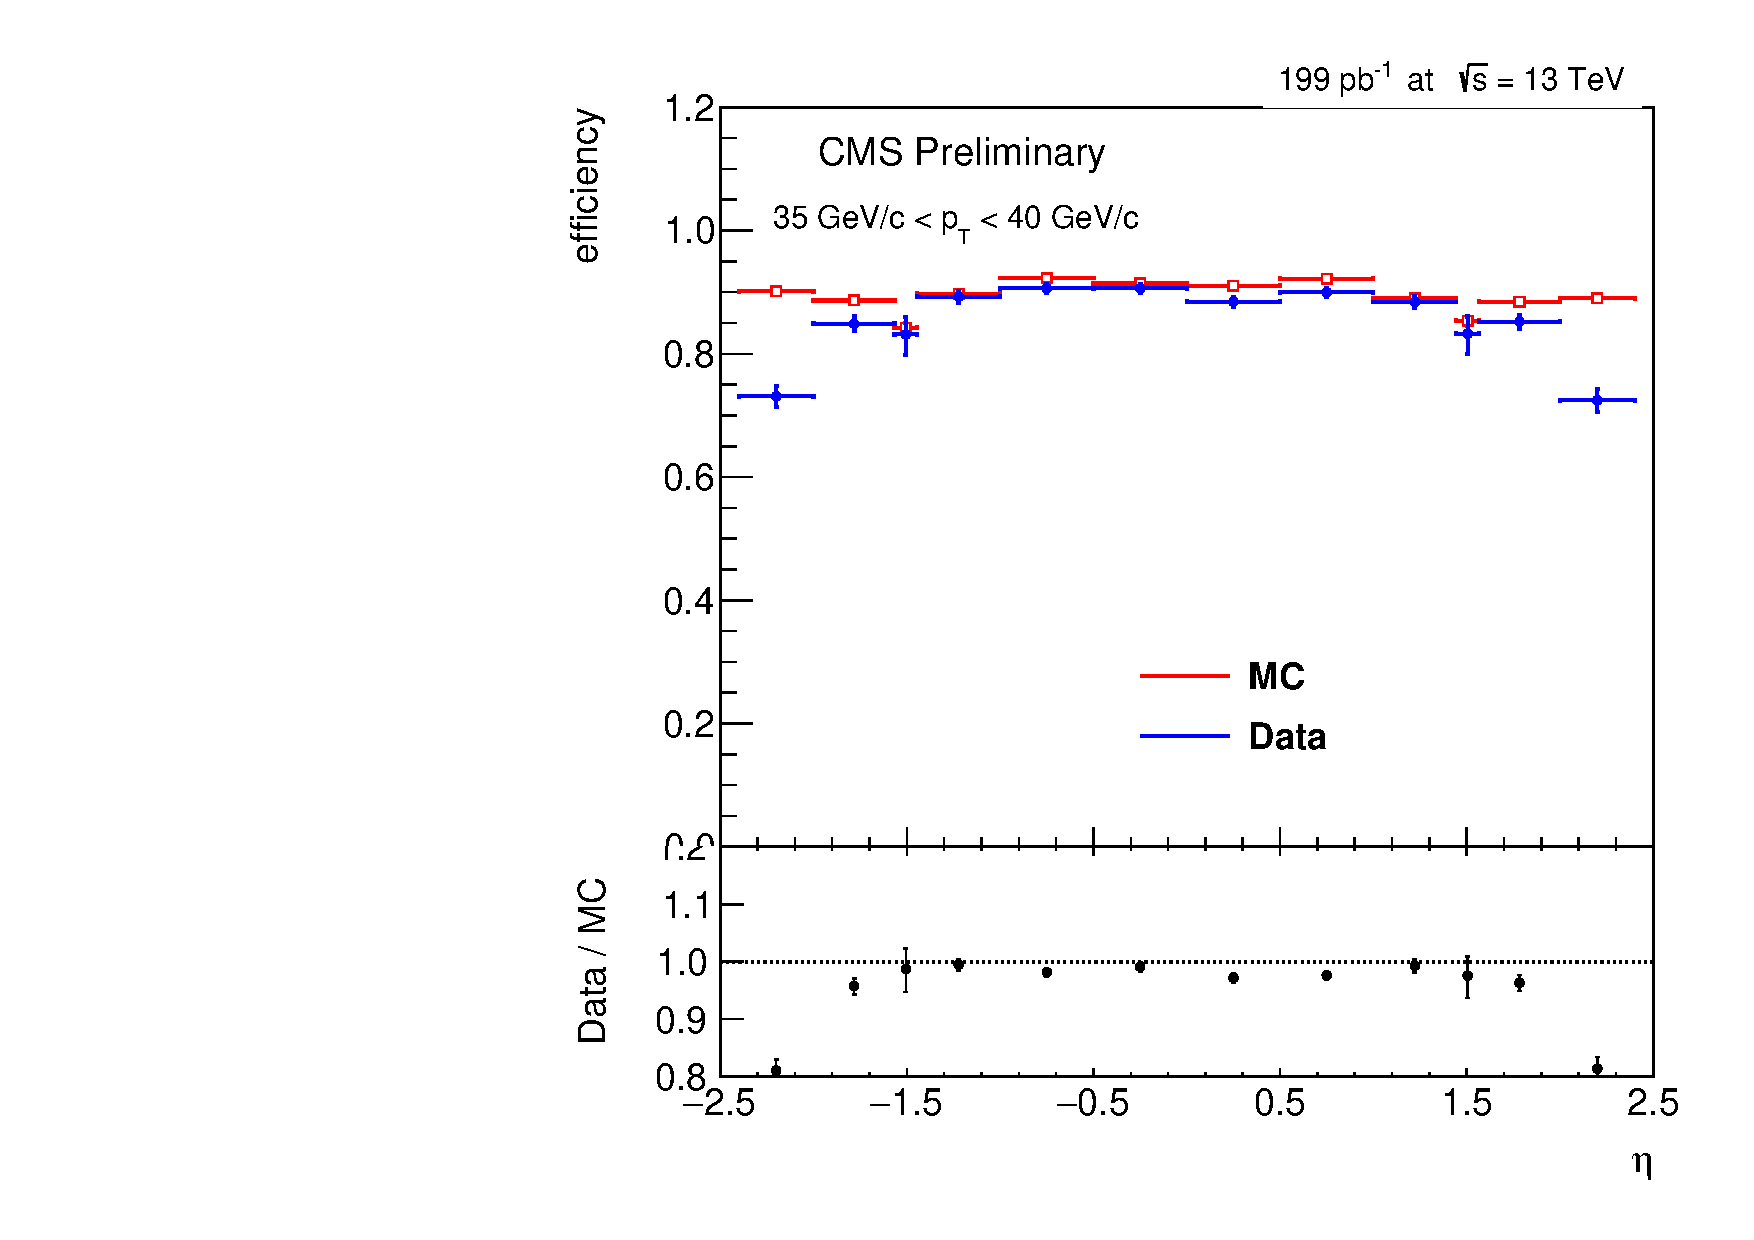
\includegraphics[width=0.45\linewidth]{plots/efficiency/13_zeehlt_positive/PtBins_eta_pt6.pdf}
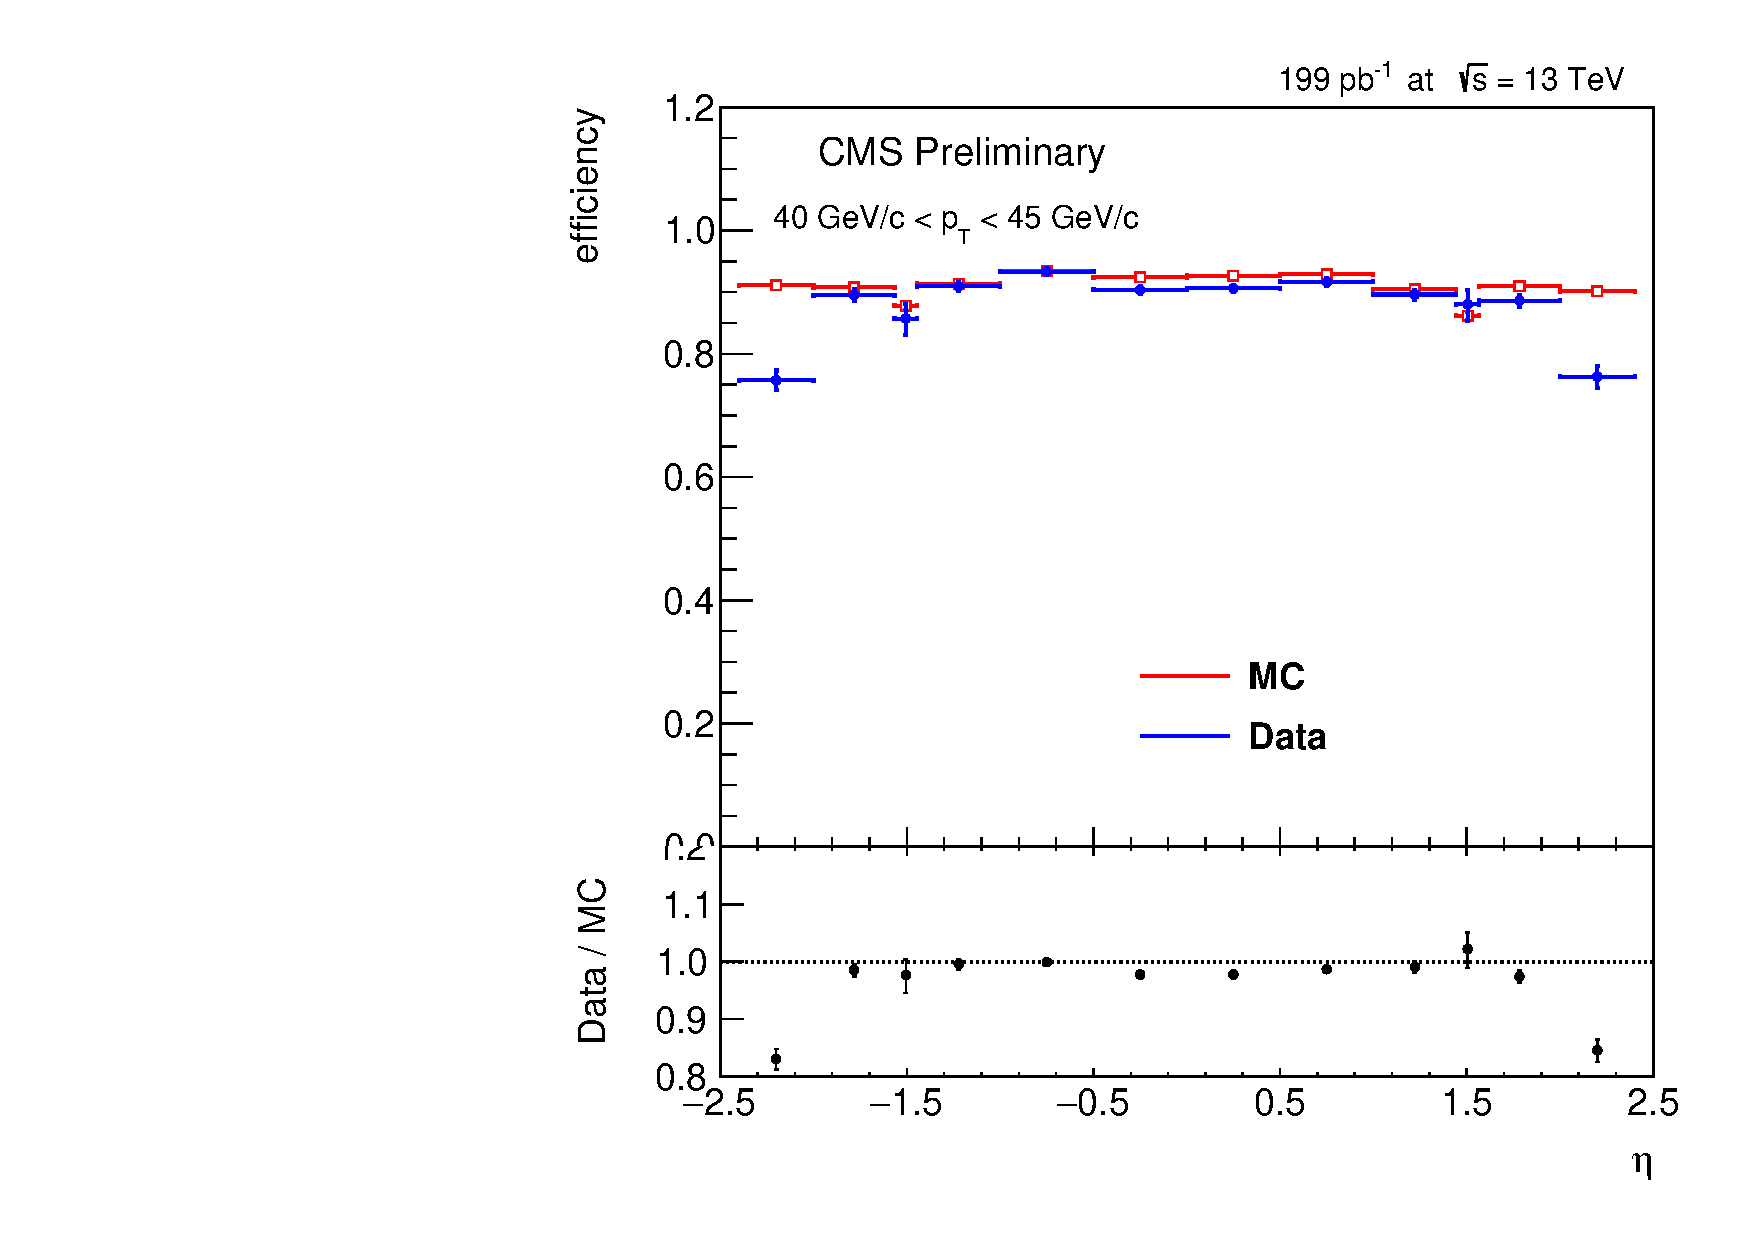
\includegraphics[width=0.45\linewidth]{plots/efficiency/13_zeehlt_positive/PtBins_eta_pt7.pdf}
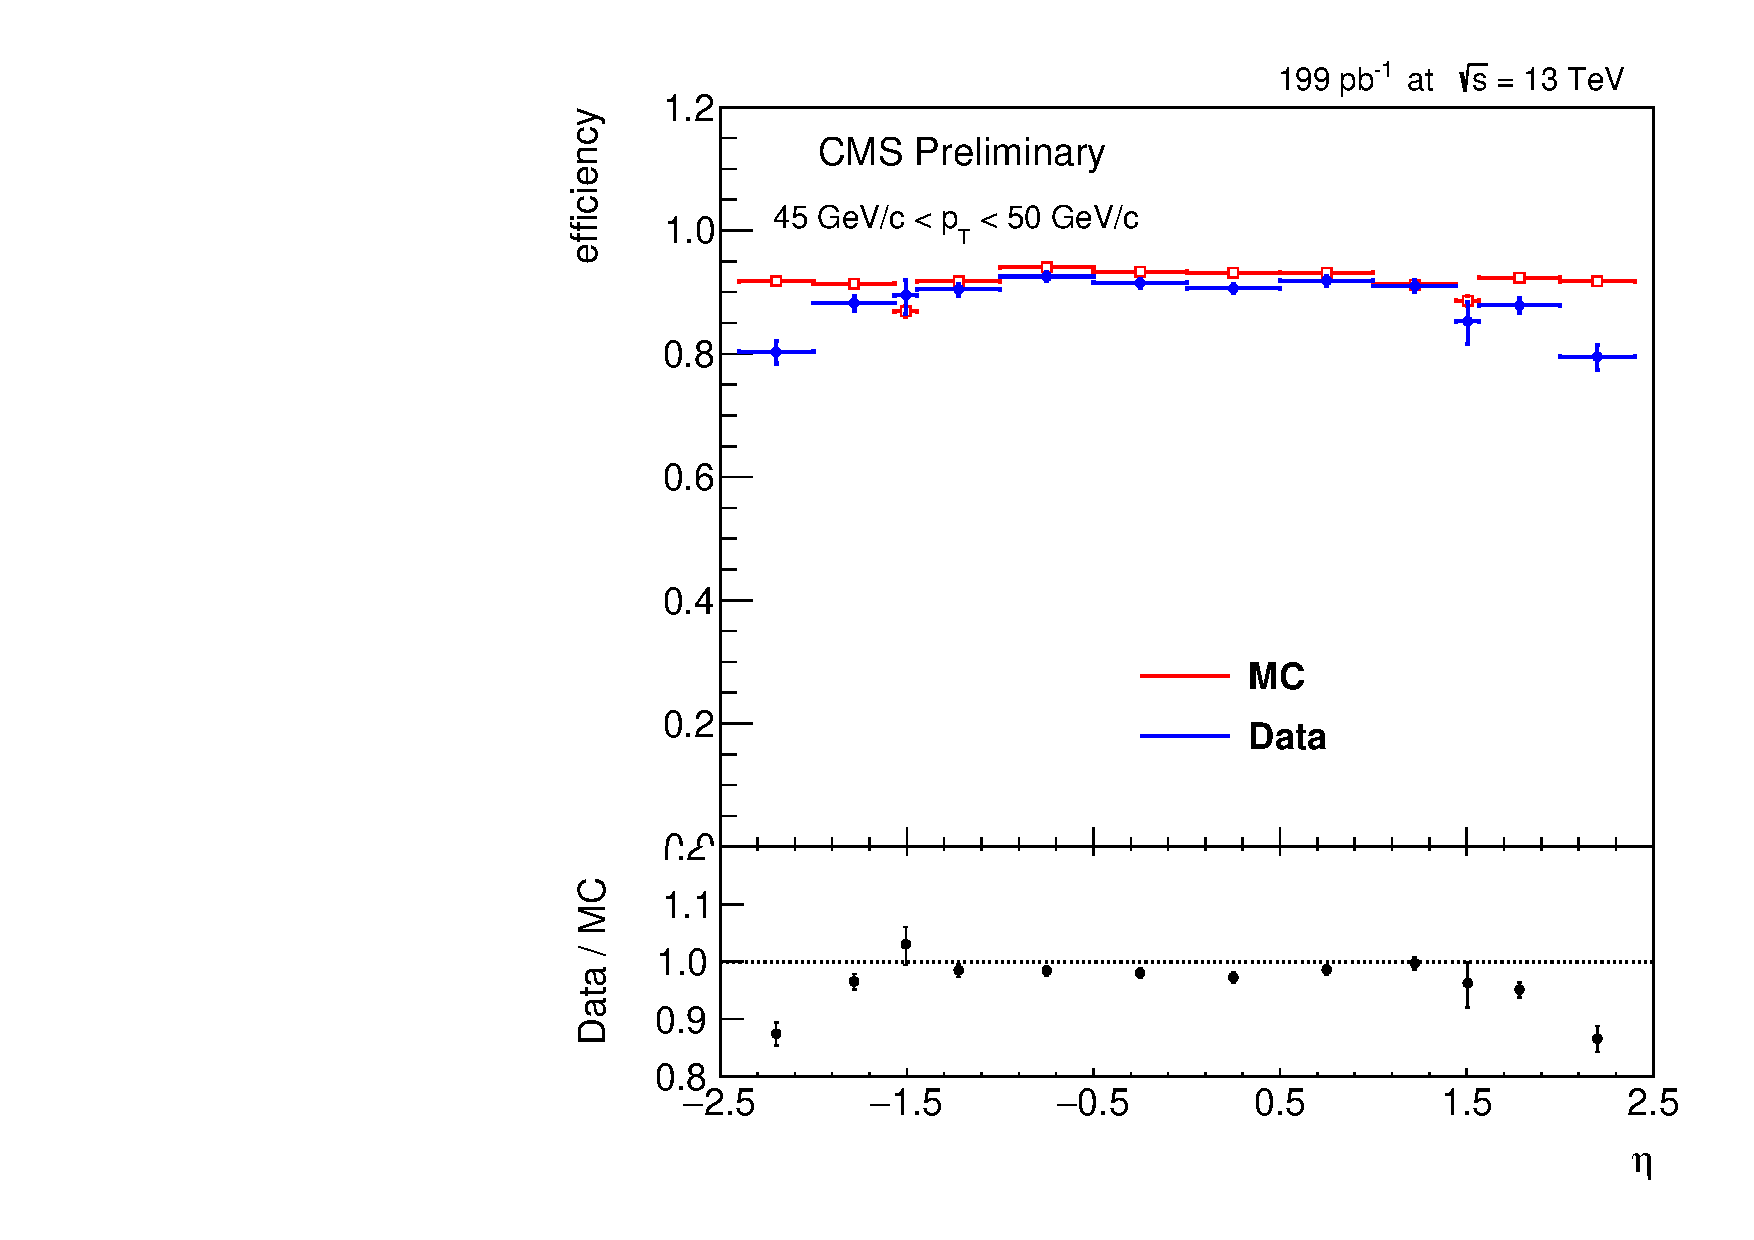
\includegraphics[width=0.45\linewidth]{plots/efficiency/13_zeehlt_positive/PtBins_eta_pt8.pdf}
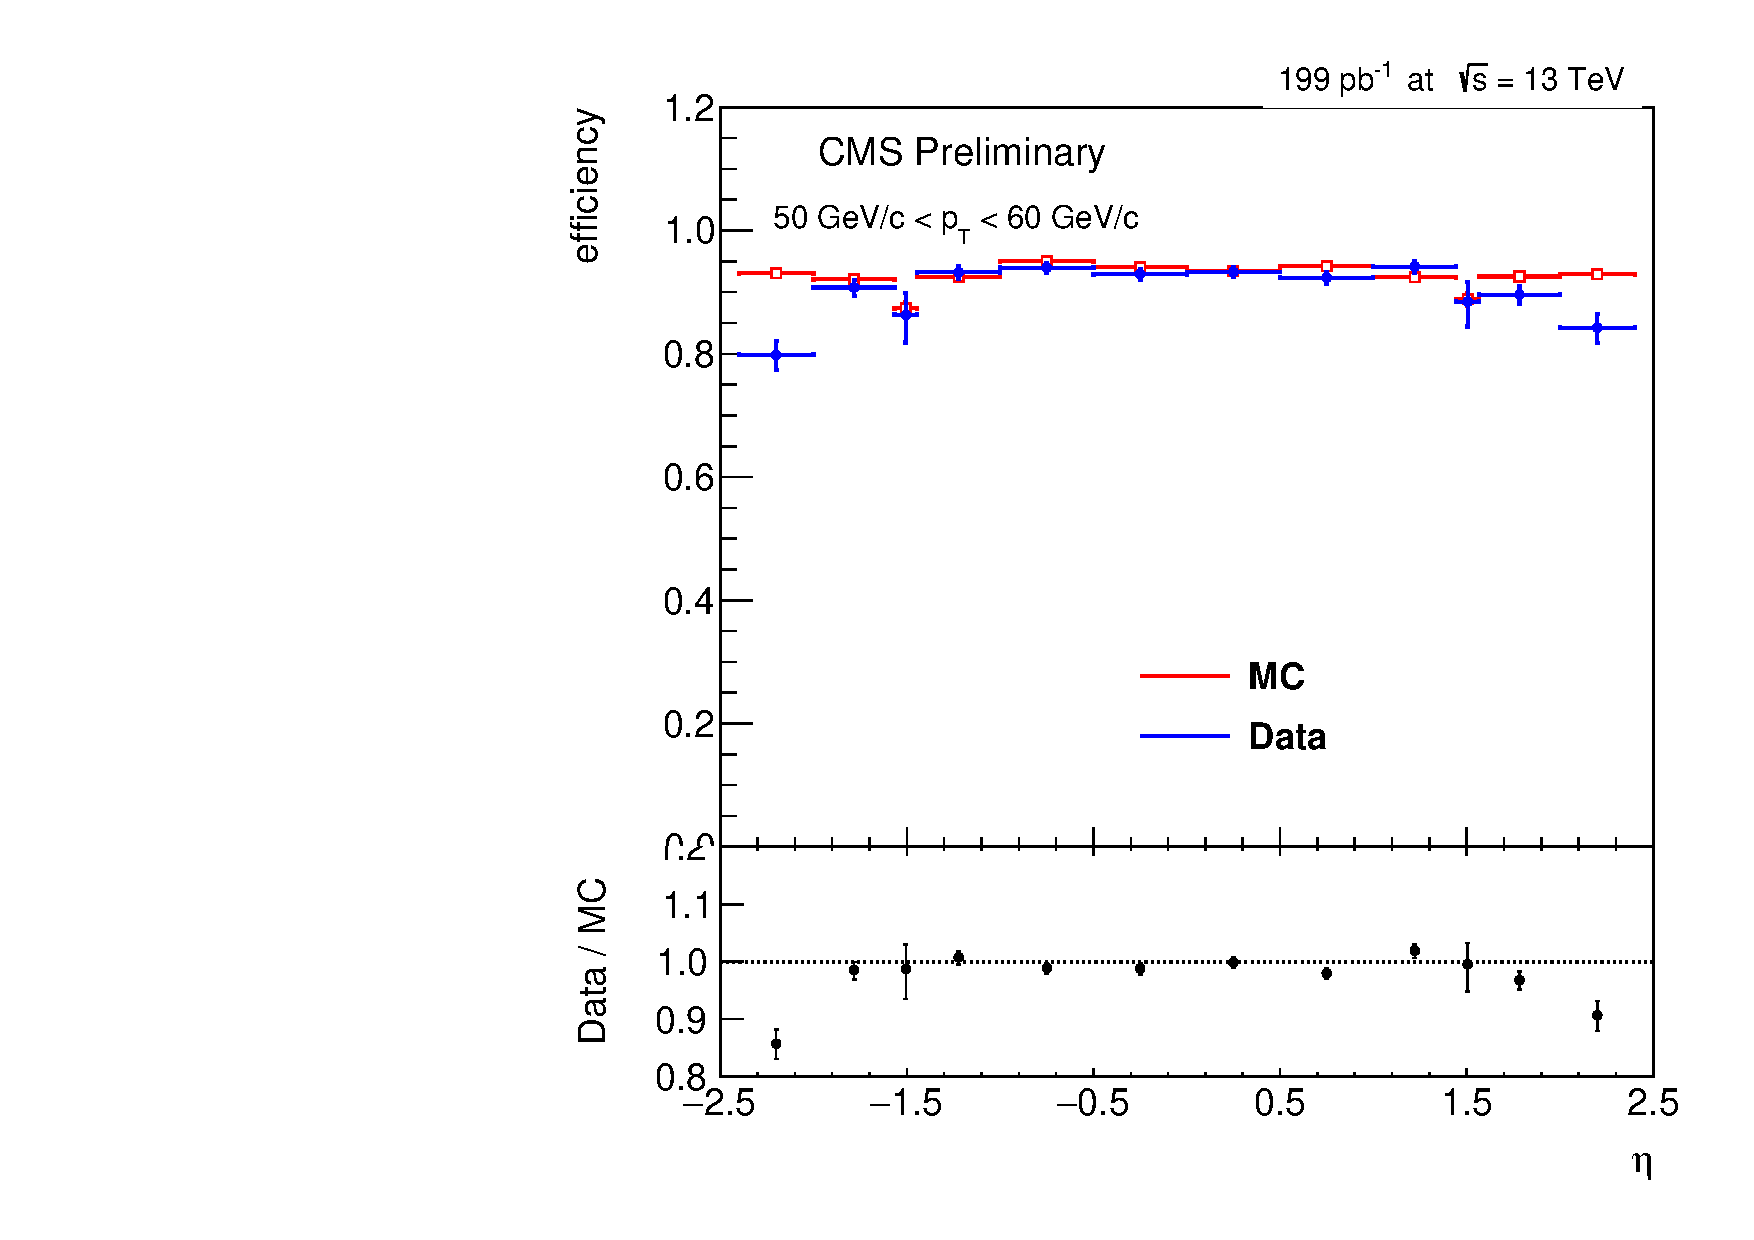
\includegraphics[width=0.45\linewidth]{plots/efficiency/13_zeehlt_positive/PtBins_eta_pt9.pdf}
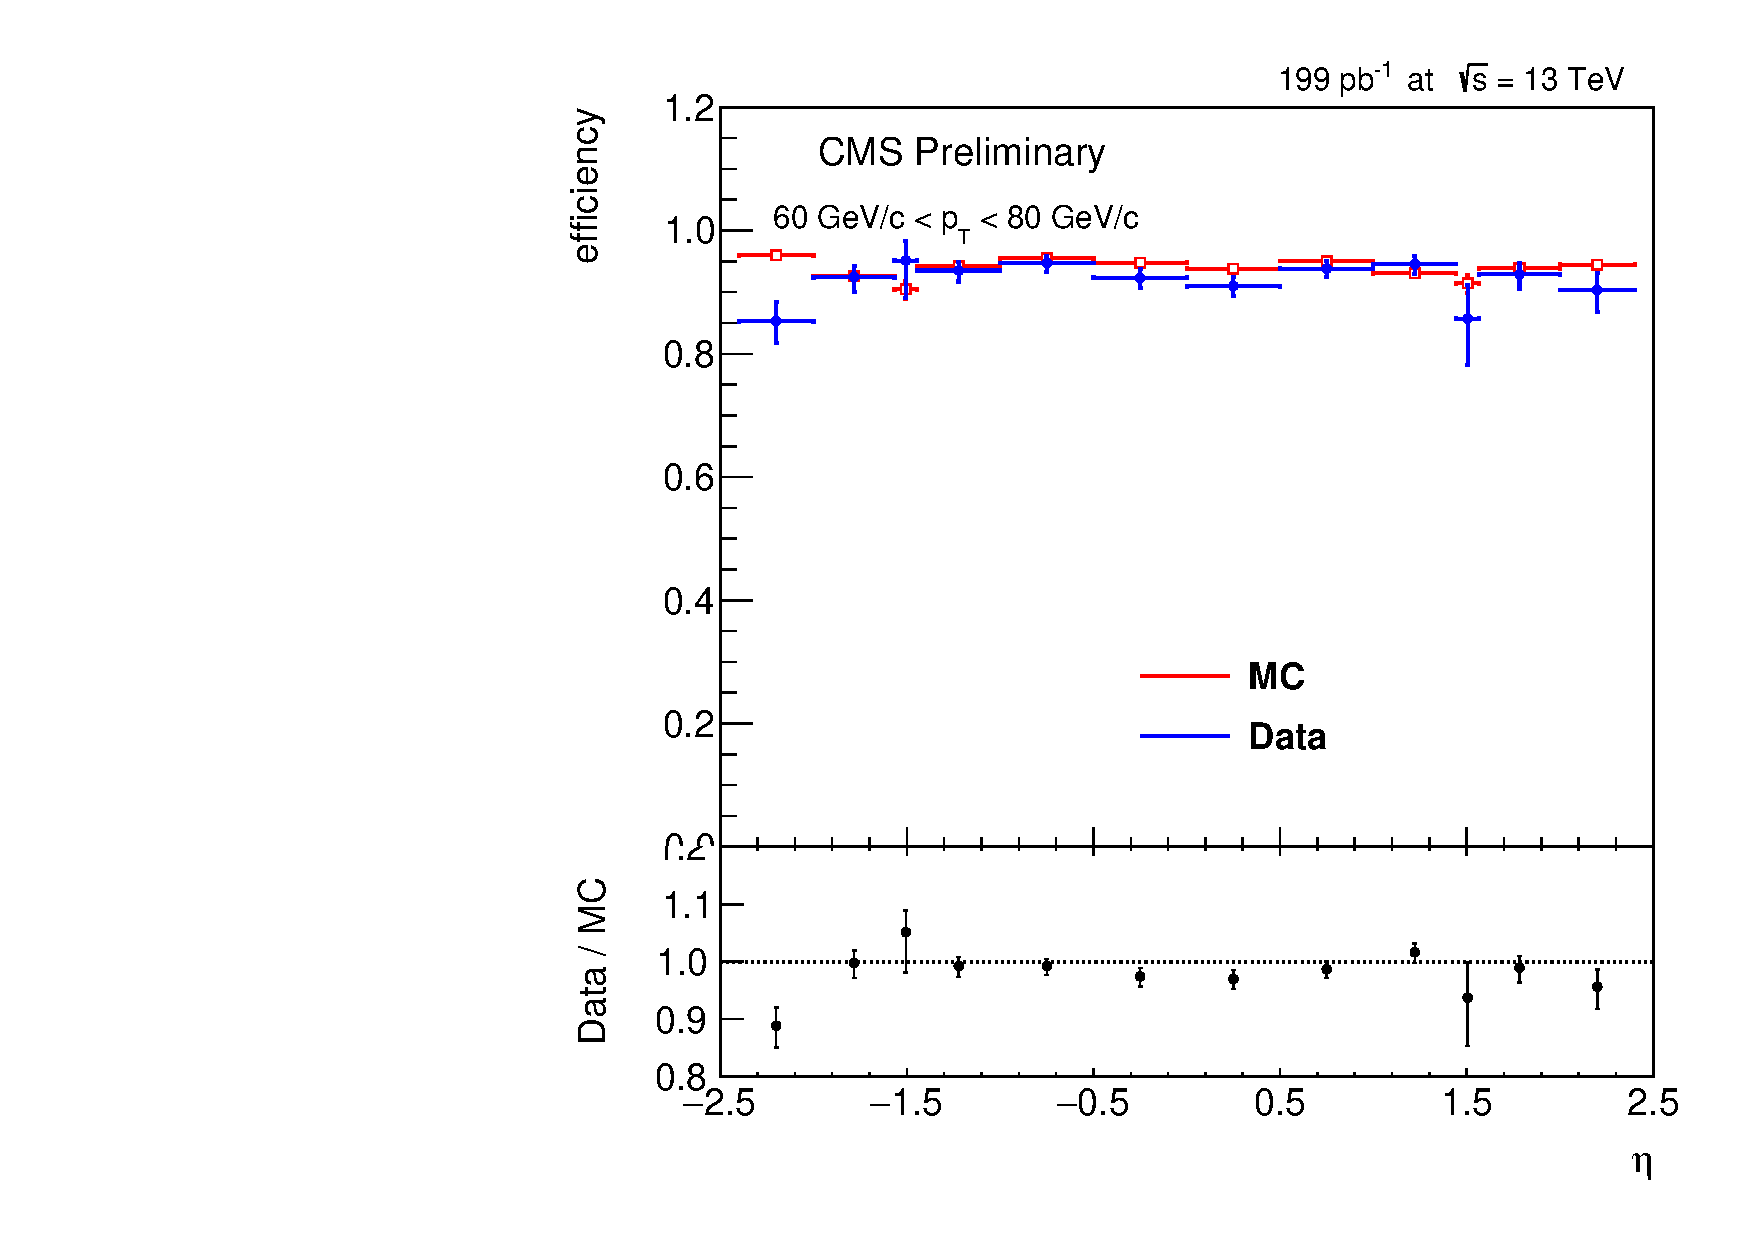
\includegraphics[width=0.45\linewidth]{plots/efficiency/13_zeehlt_positive/PtBins_eta_pt10.pdf}
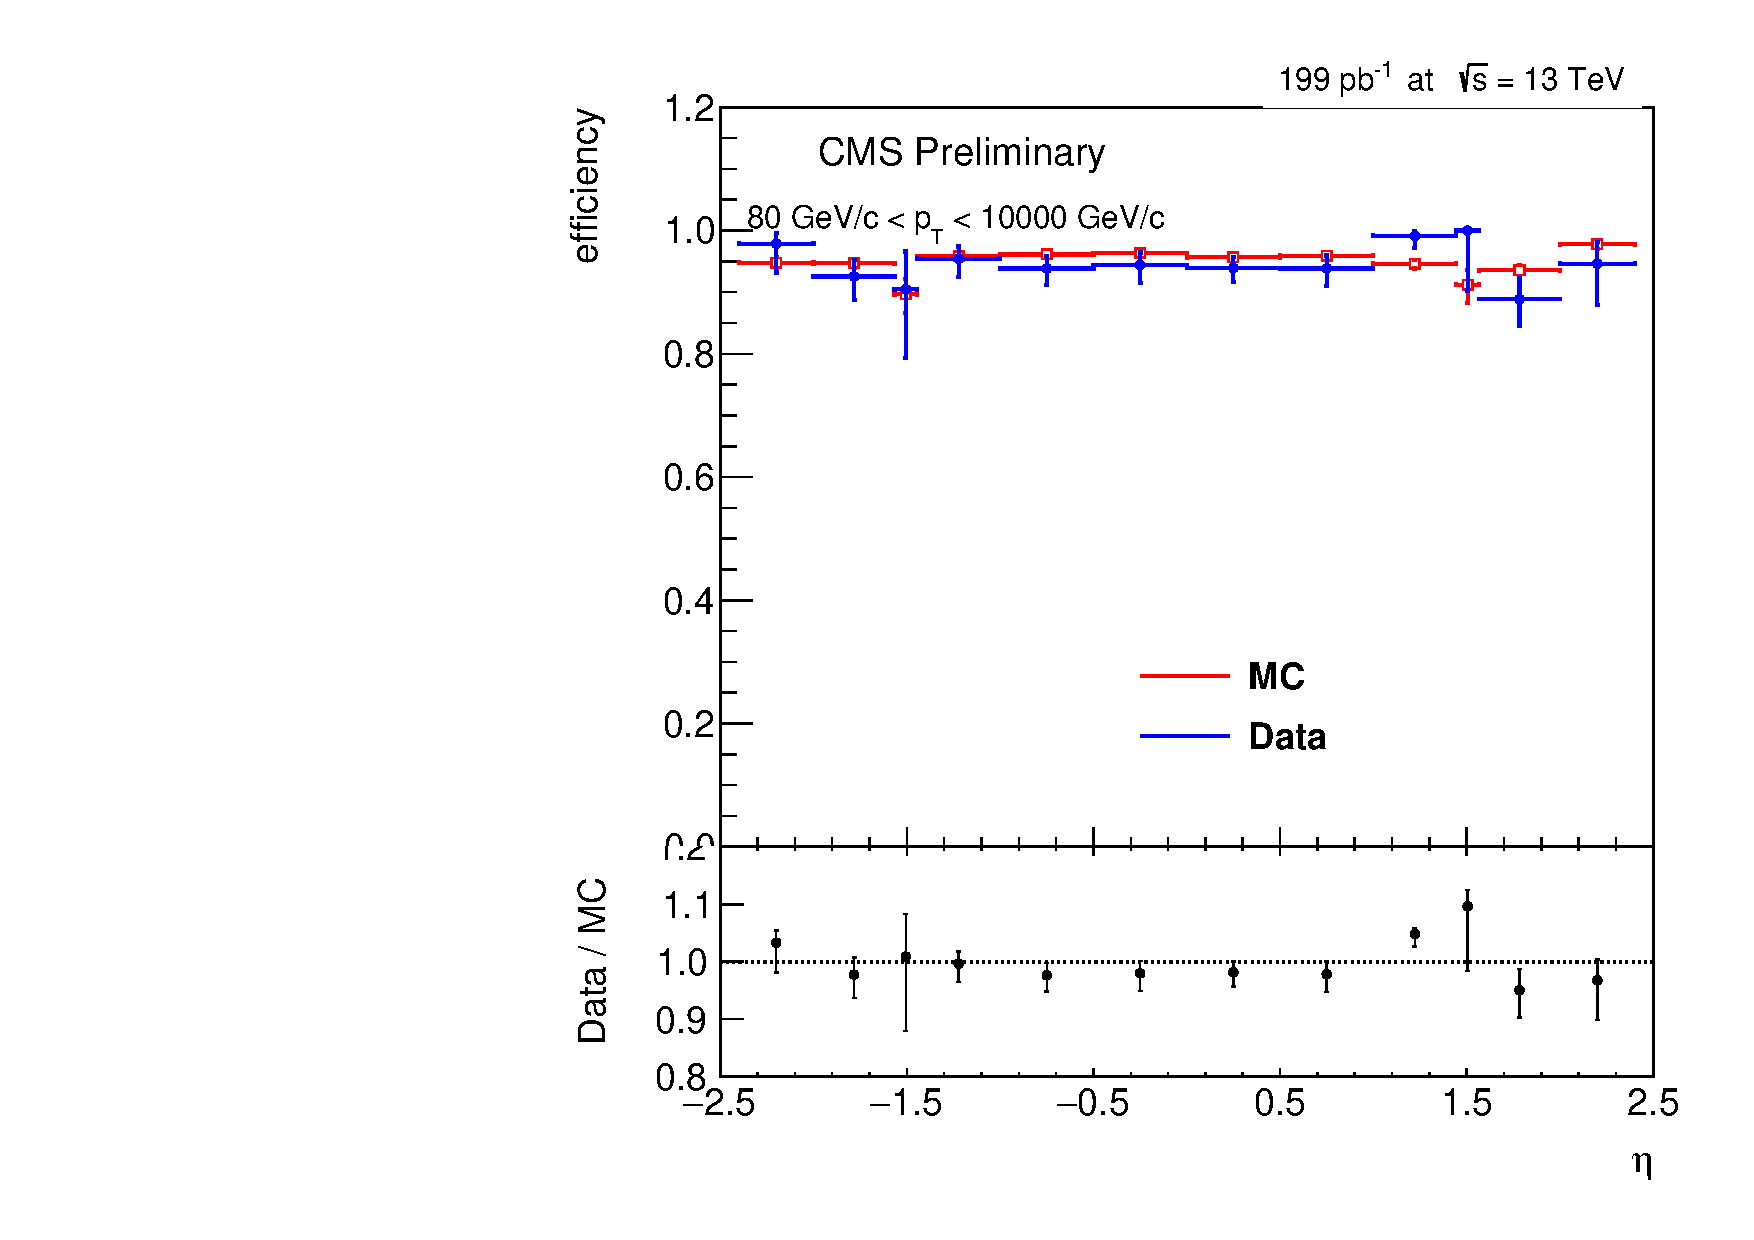
\includegraphics[width=0.45\linewidth]{plots/efficiency/13_zeehlt_positive/PtBins_eta_pt11.pdf}
\caption{$\eta$ dependence of Single electron trigger efficiency scale factors, separated by $p_T$ bins, for positively charged electrons in the 13 TeV samples.}
\label{fig:Eff:el:13:HLT:pos}
\end{figure}
\begin{figure}
\centering
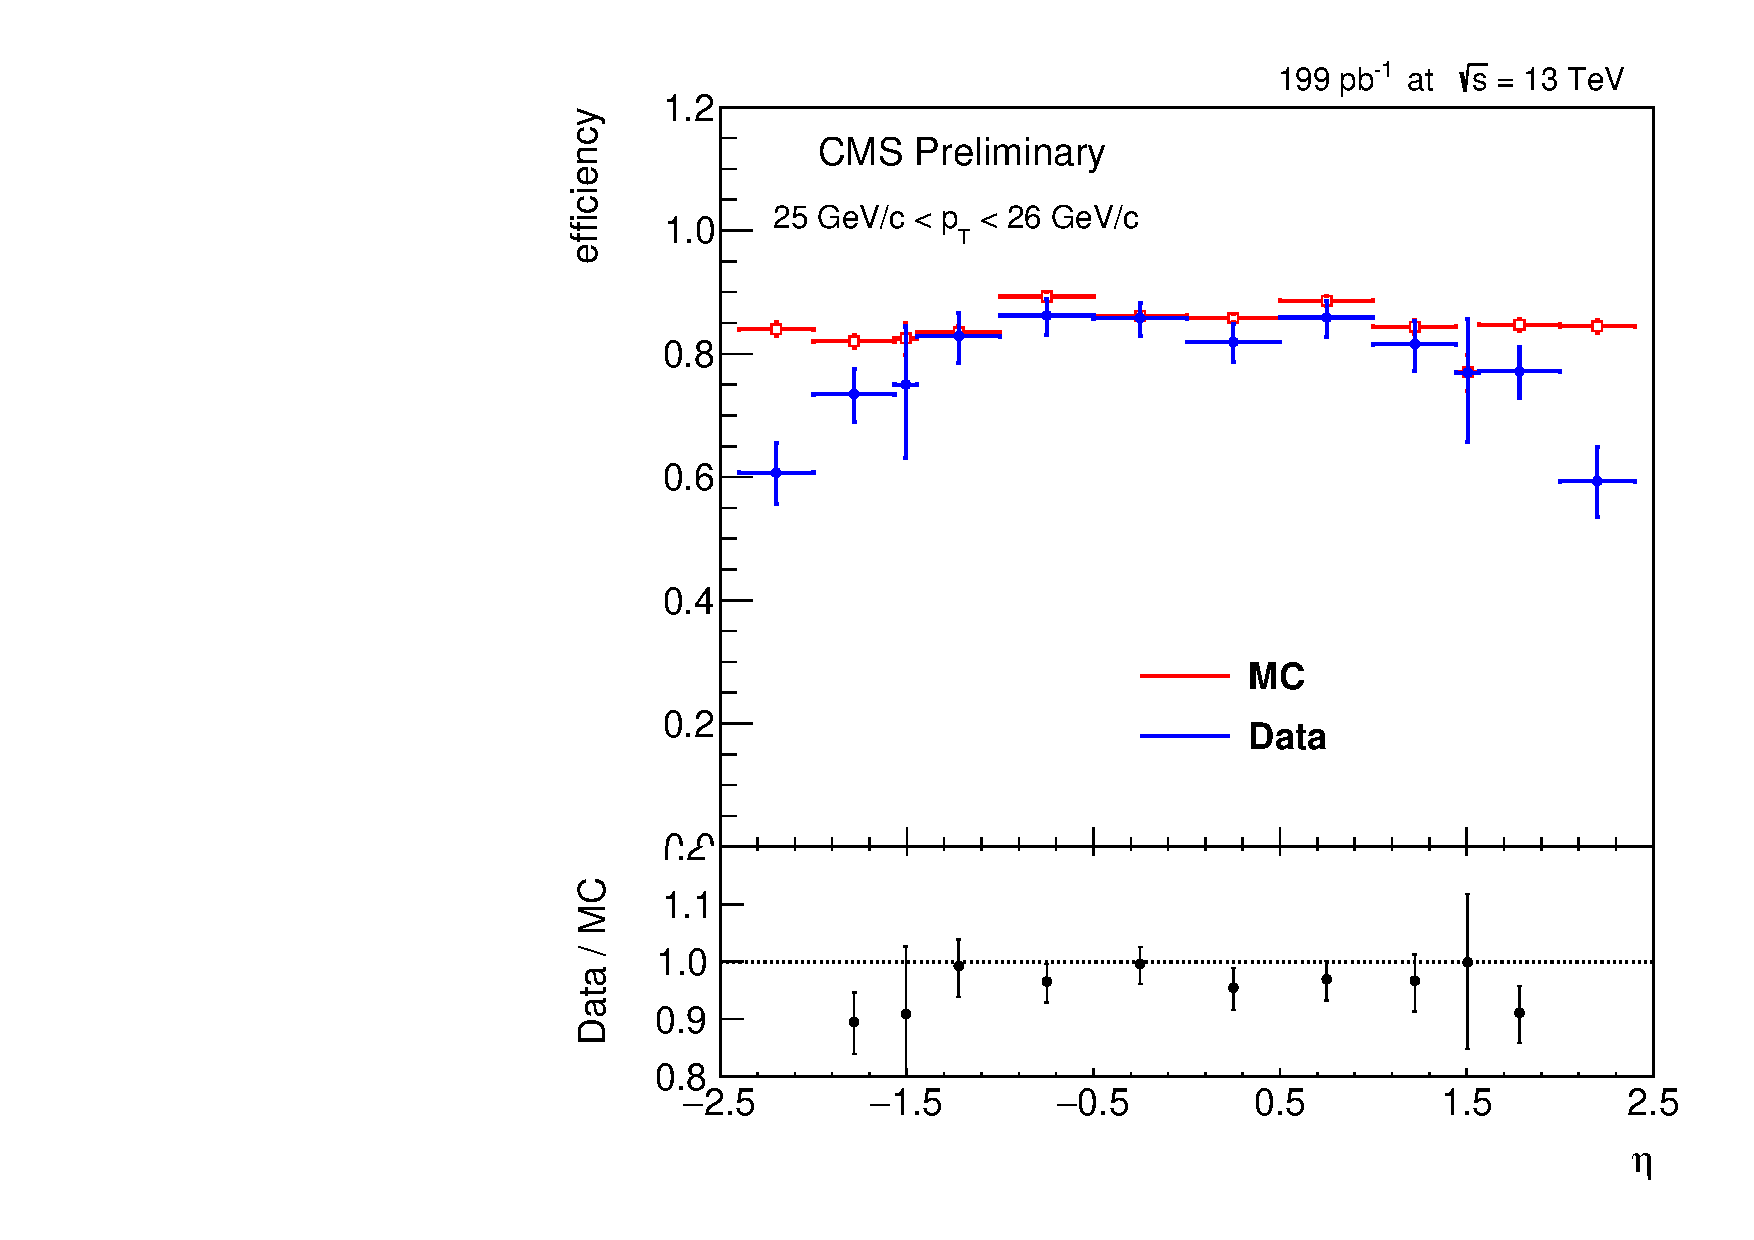
\includegraphics[width=0.45\linewidth]{plots/efficiency/13_zeehlt_negative/PtBins_eta_pt0.pdf}
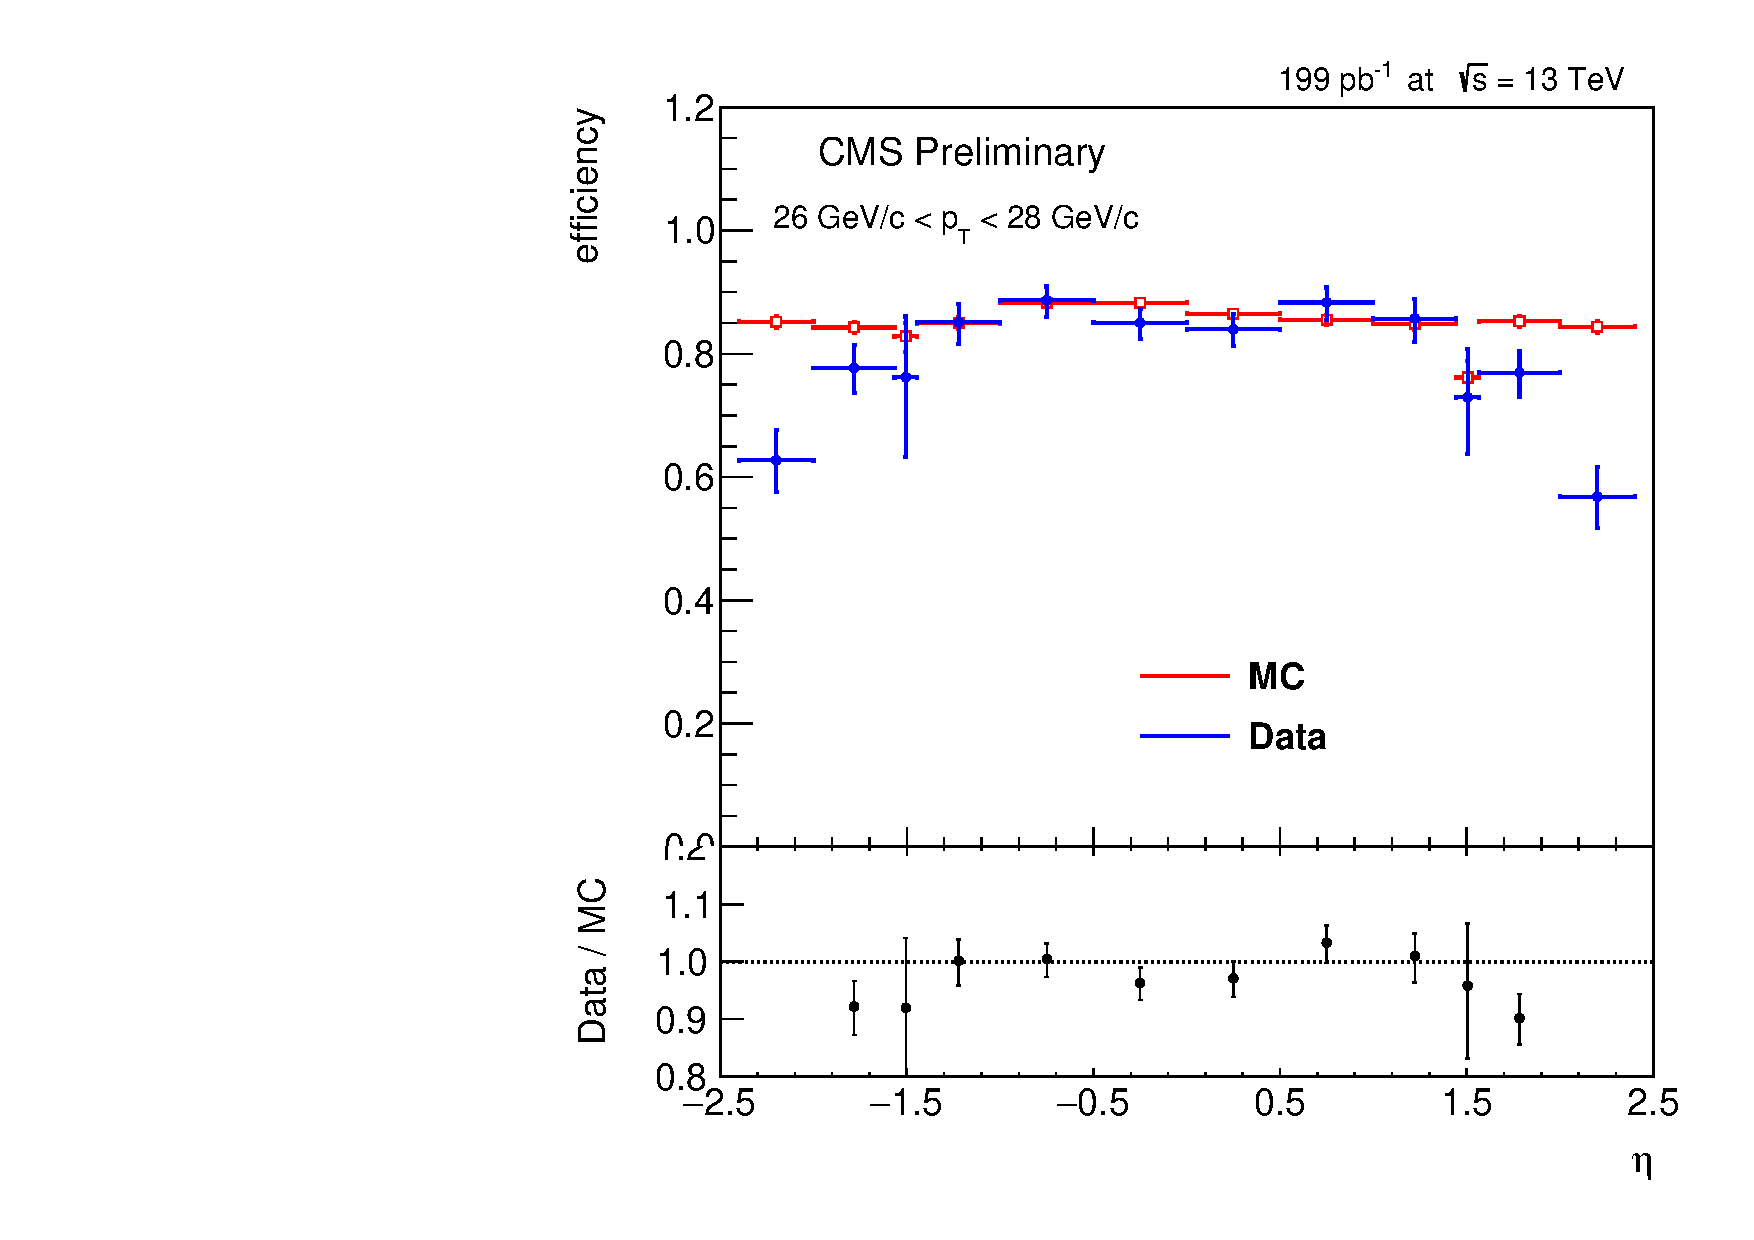
\includegraphics[width=0.45\linewidth]{plots/efficiency/13_zeehlt_negative/PtBins_eta_pt1.pdf}
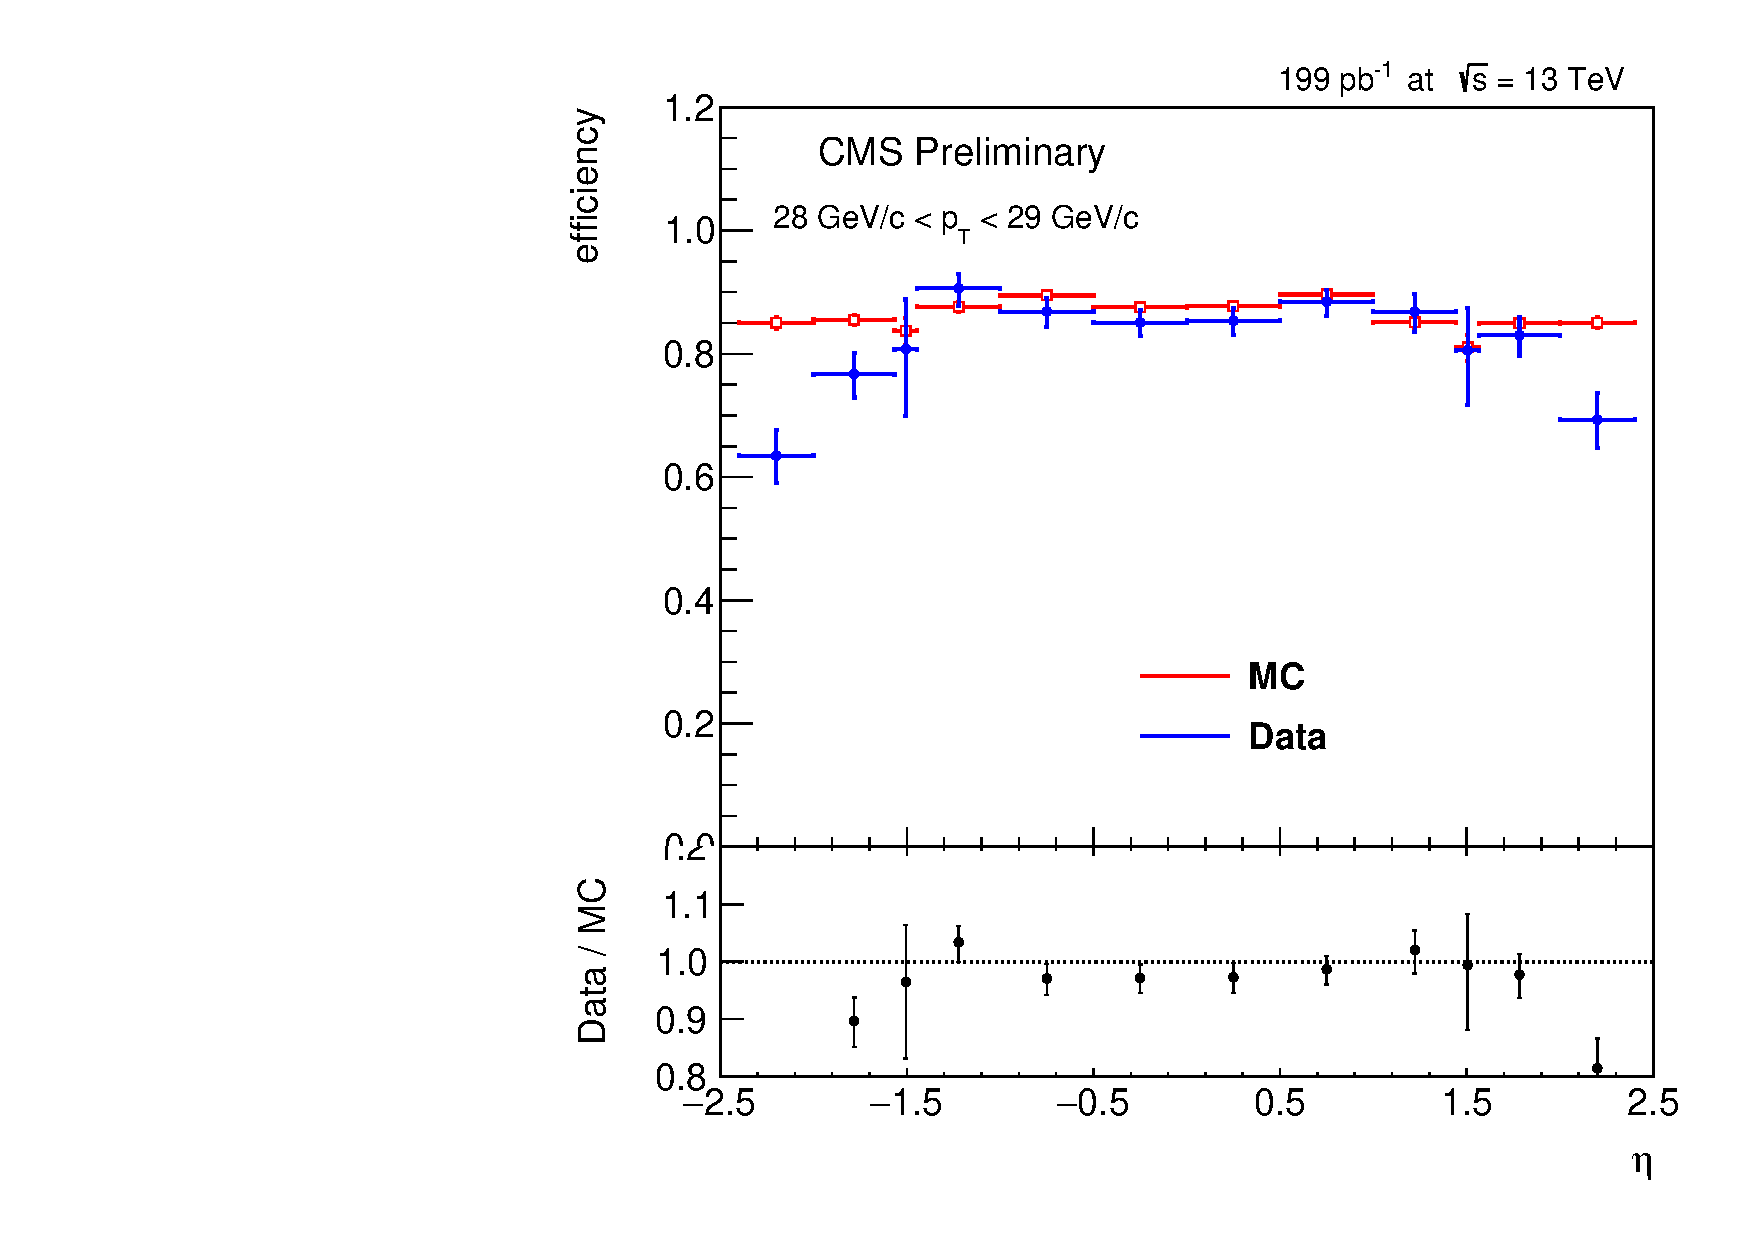
\includegraphics[width=0.45\linewidth]{plots/efficiency/13_zeehlt_negative/PtBins_eta_pt2.pdf}
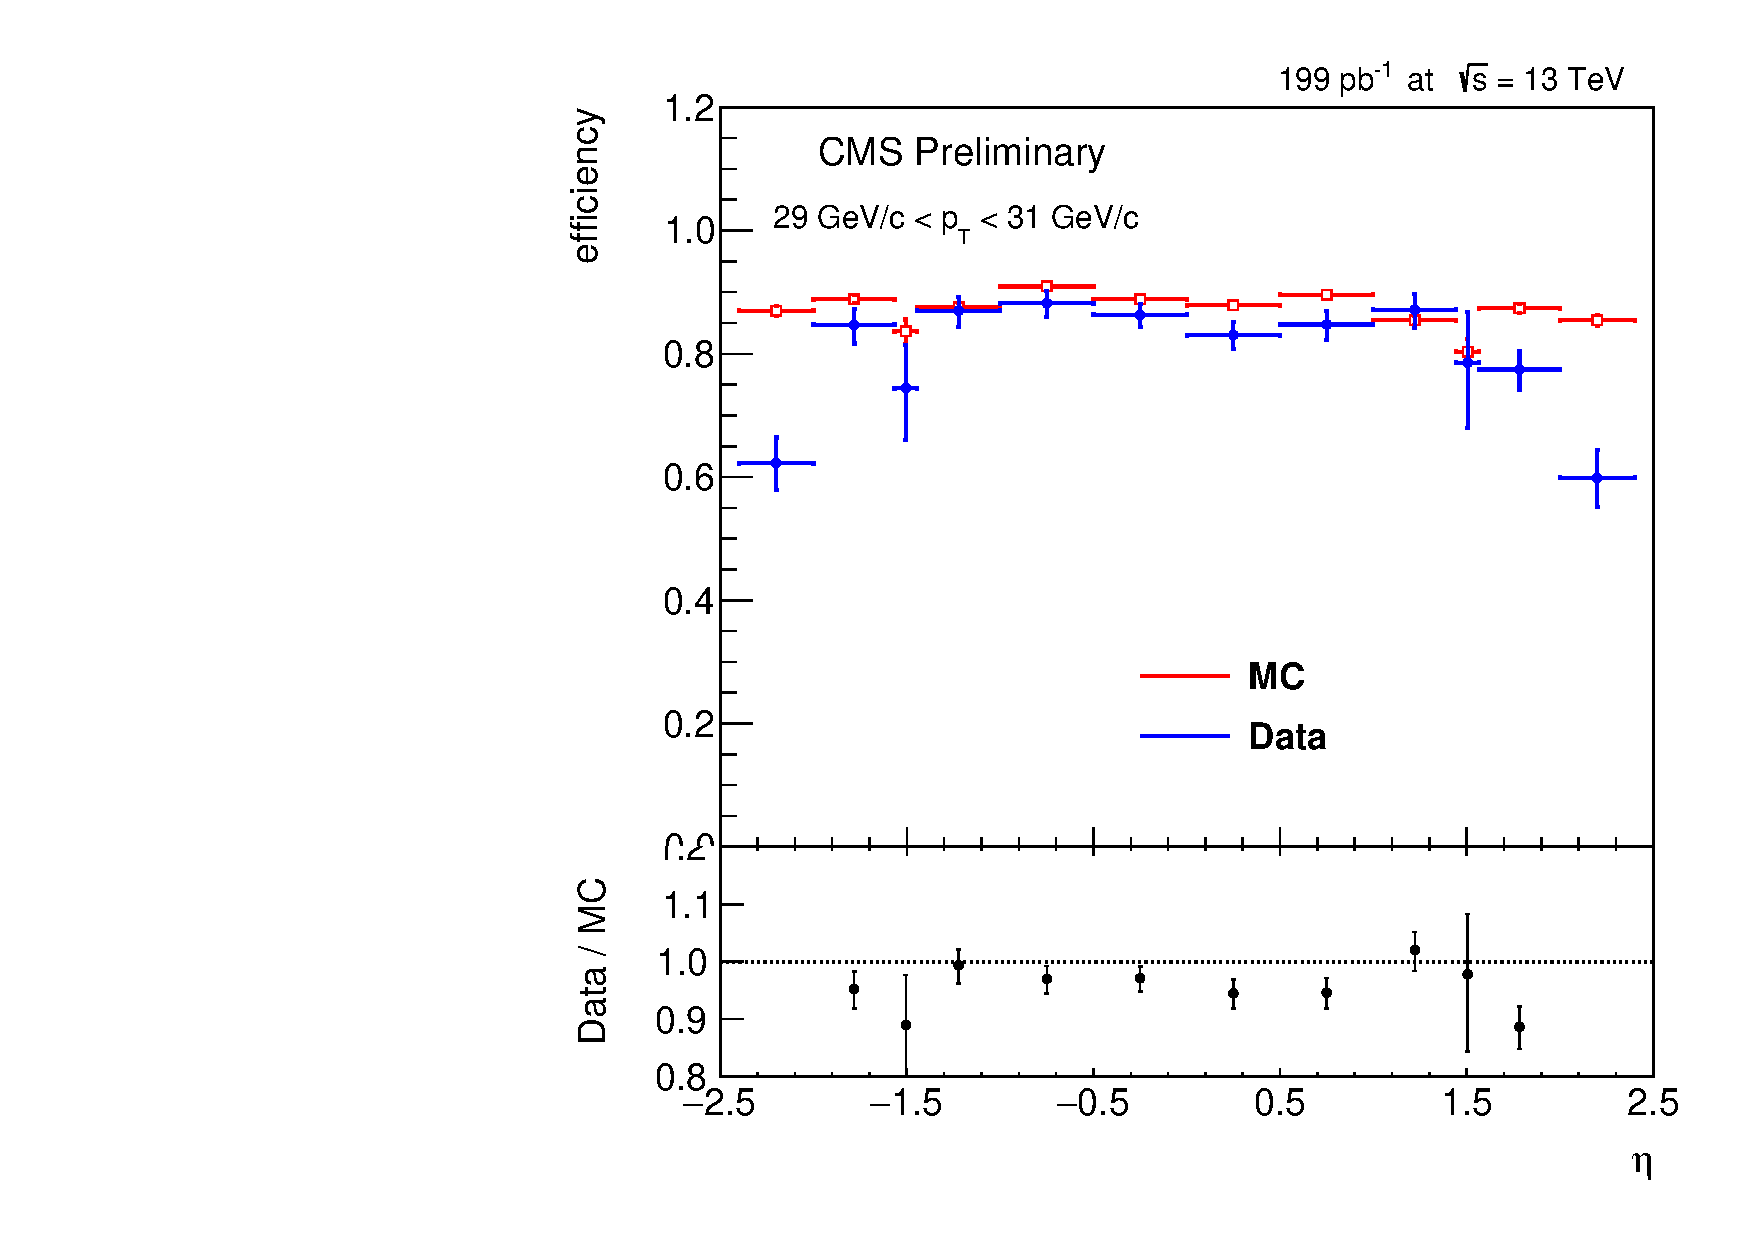
\includegraphics[width=0.45\linewidth]{plots/efficiency/13_zeehlt_negative/PtBins_eta_pt3.pdf}
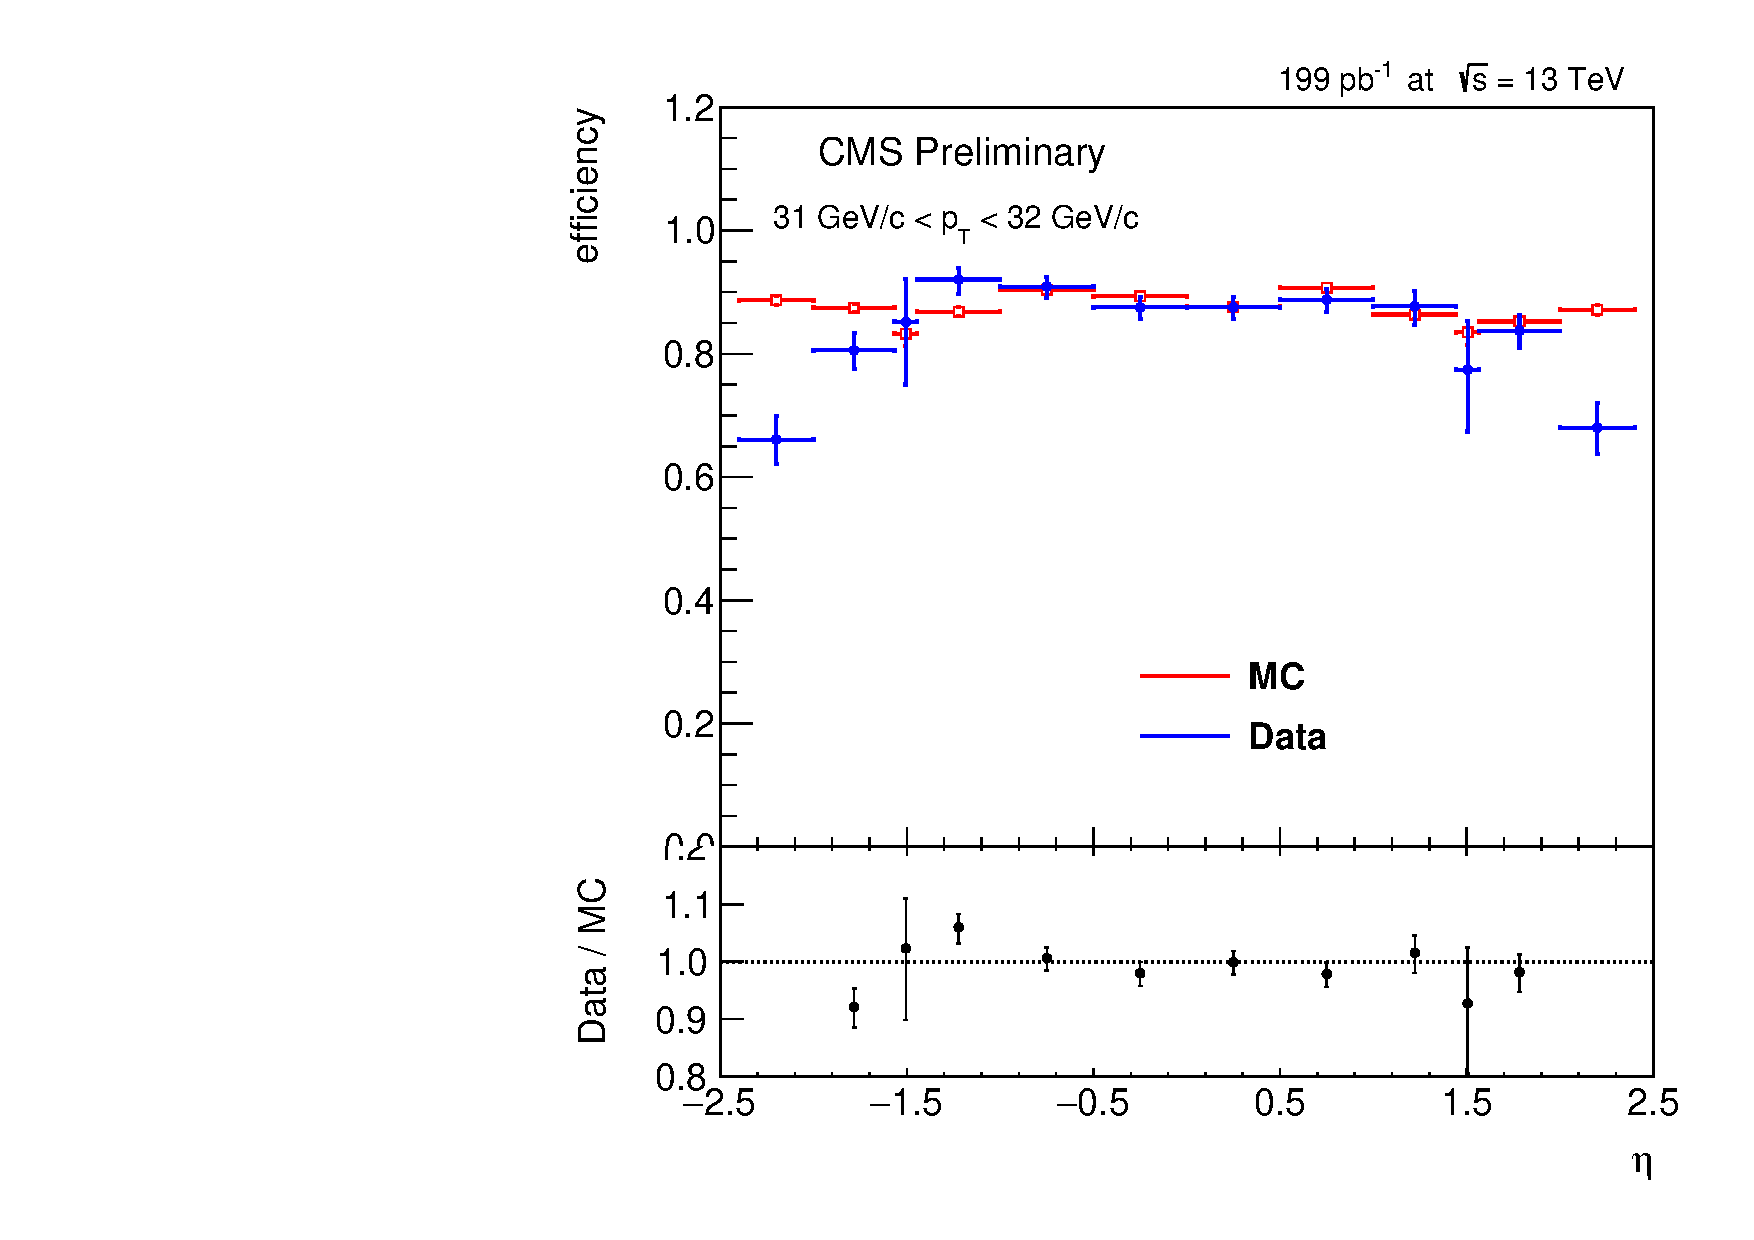
\includegraphics[width=0.45\linewidth]{plots/efficiency/13_zeehlt_negative/PtBins_eta_pt4.pdf}
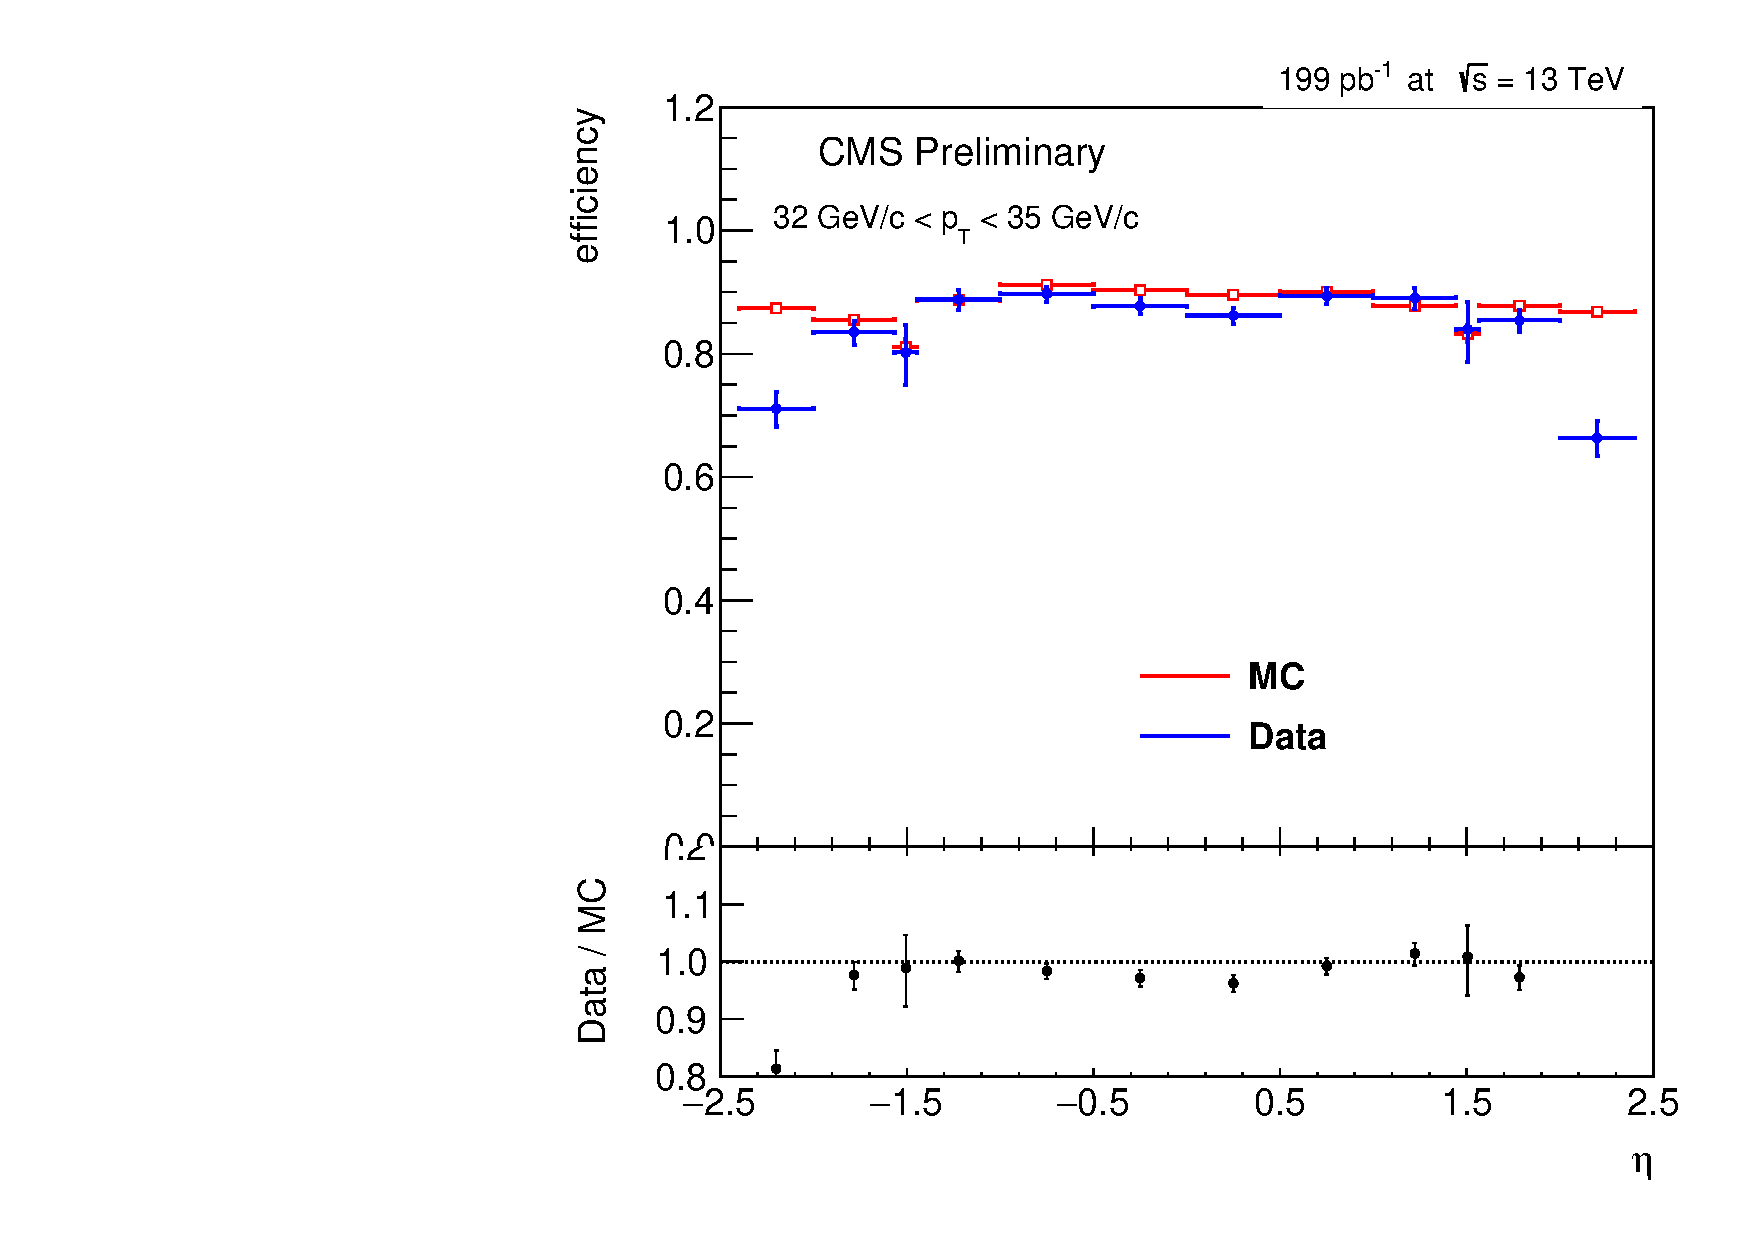
\includegraphics[width=0.45\linewidth]{plots/efficiency/13_zeehlt_negative/PtBins_eta_pt5.pdf}
\caption{$\eta$ dependence of Single electron trigger efficiency scale factors, separated by $p_T$ bins, for negatively charged electrons in the 13 TeV samples.}
% \label{fig:Eff:el:13:HLT:neg}
\end{figure}
\begin{figure}
\ContinuedFloat
\centering
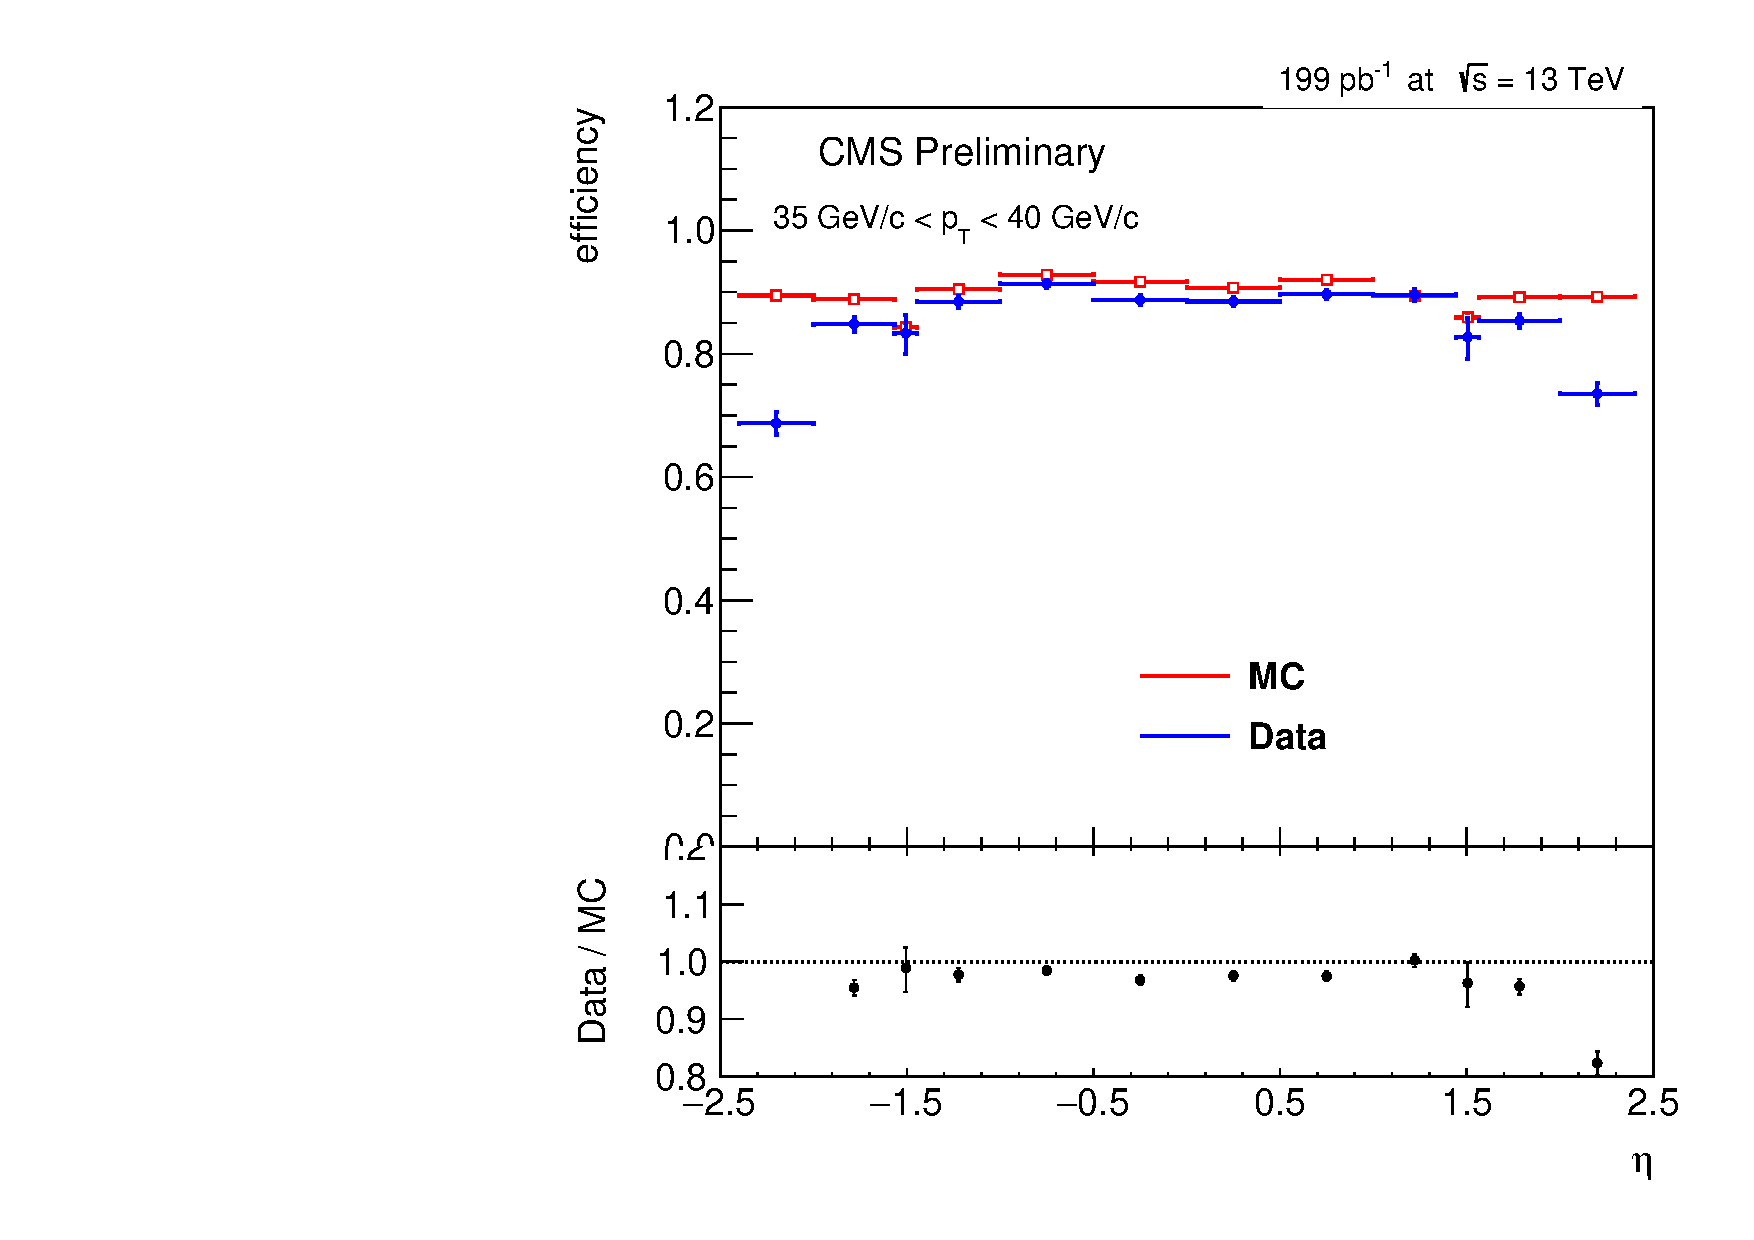
\includegraphics[width=0.45\linewidth]{plots/efficiency/13_zeehlt_negative/PtBins_eta_pt6.pdf}
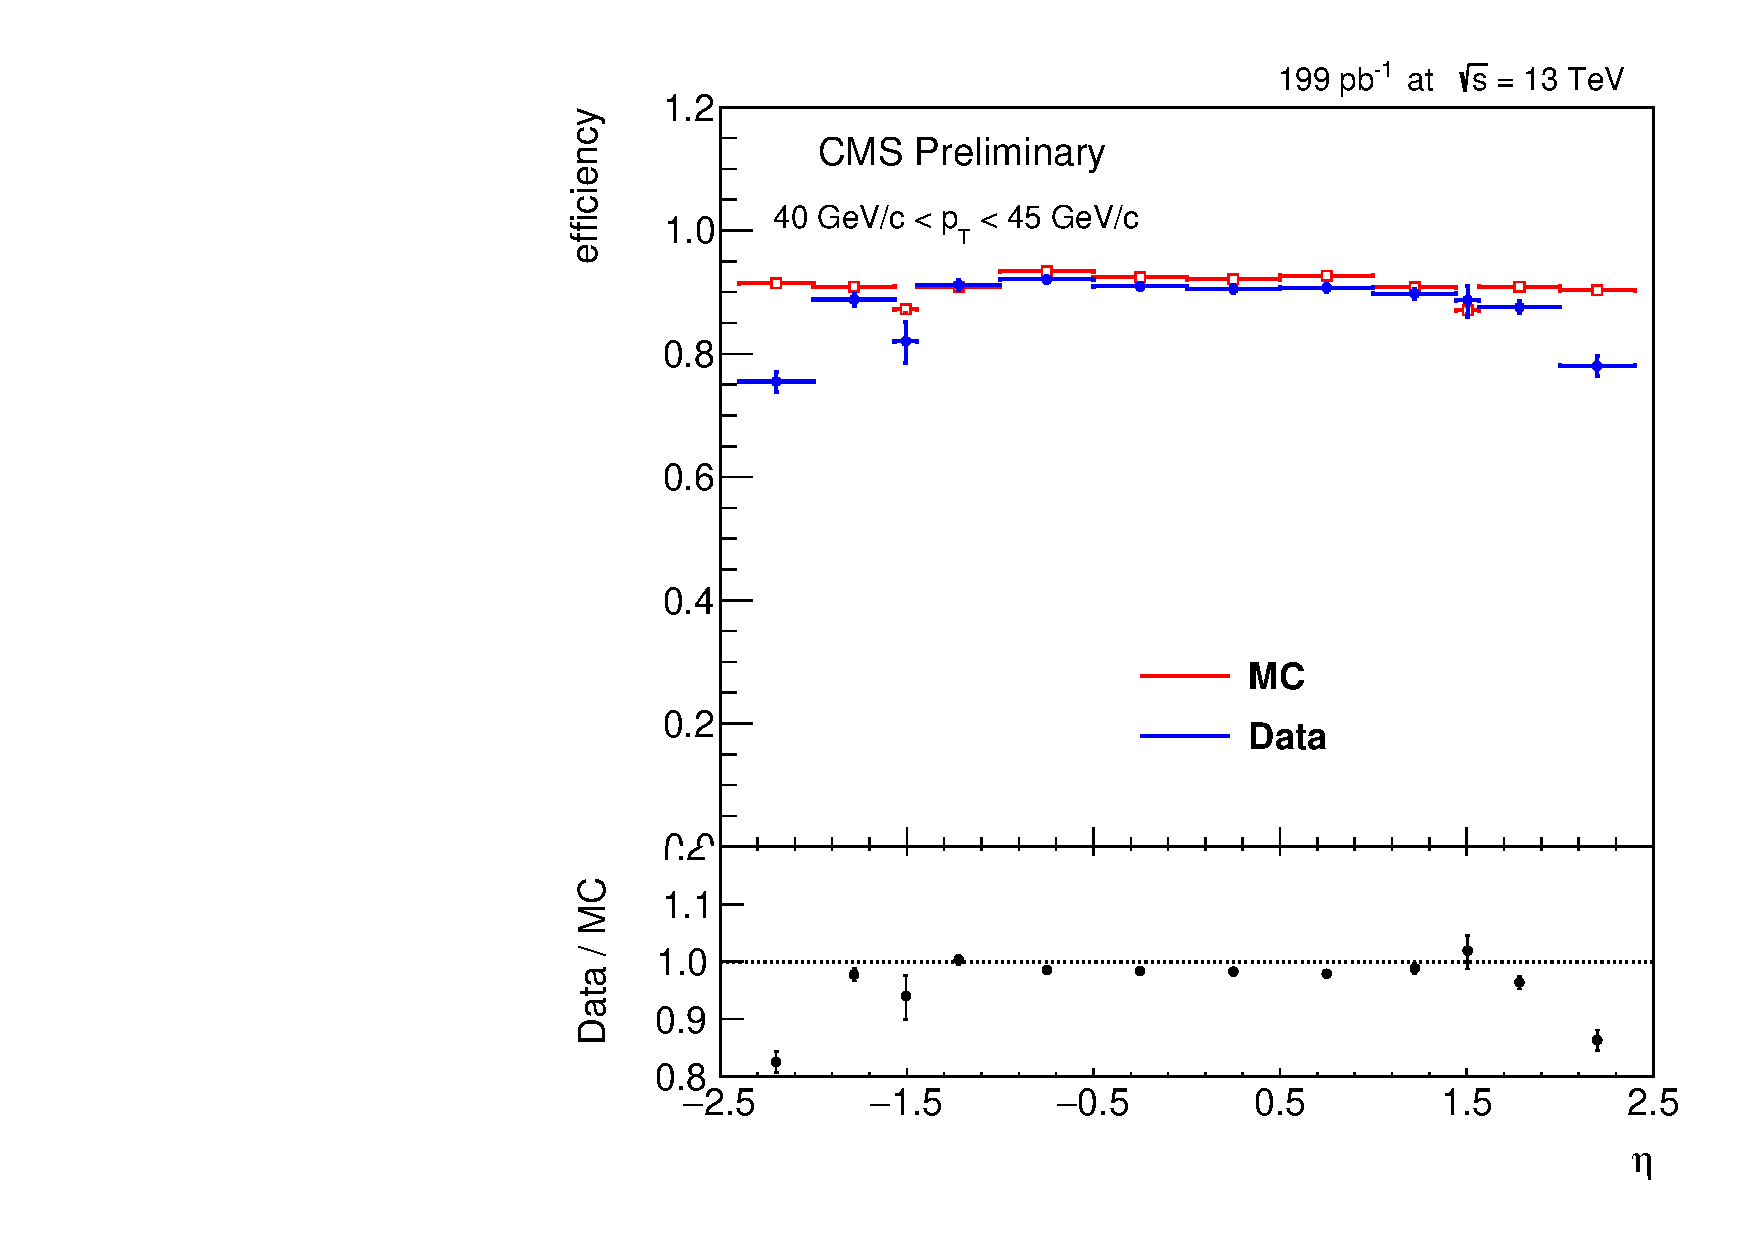
\includegraphics[width=0.45\linewidth]{plots/efficiency/13_zeehlt_negative/PtBins_eta_pt7.pdf}
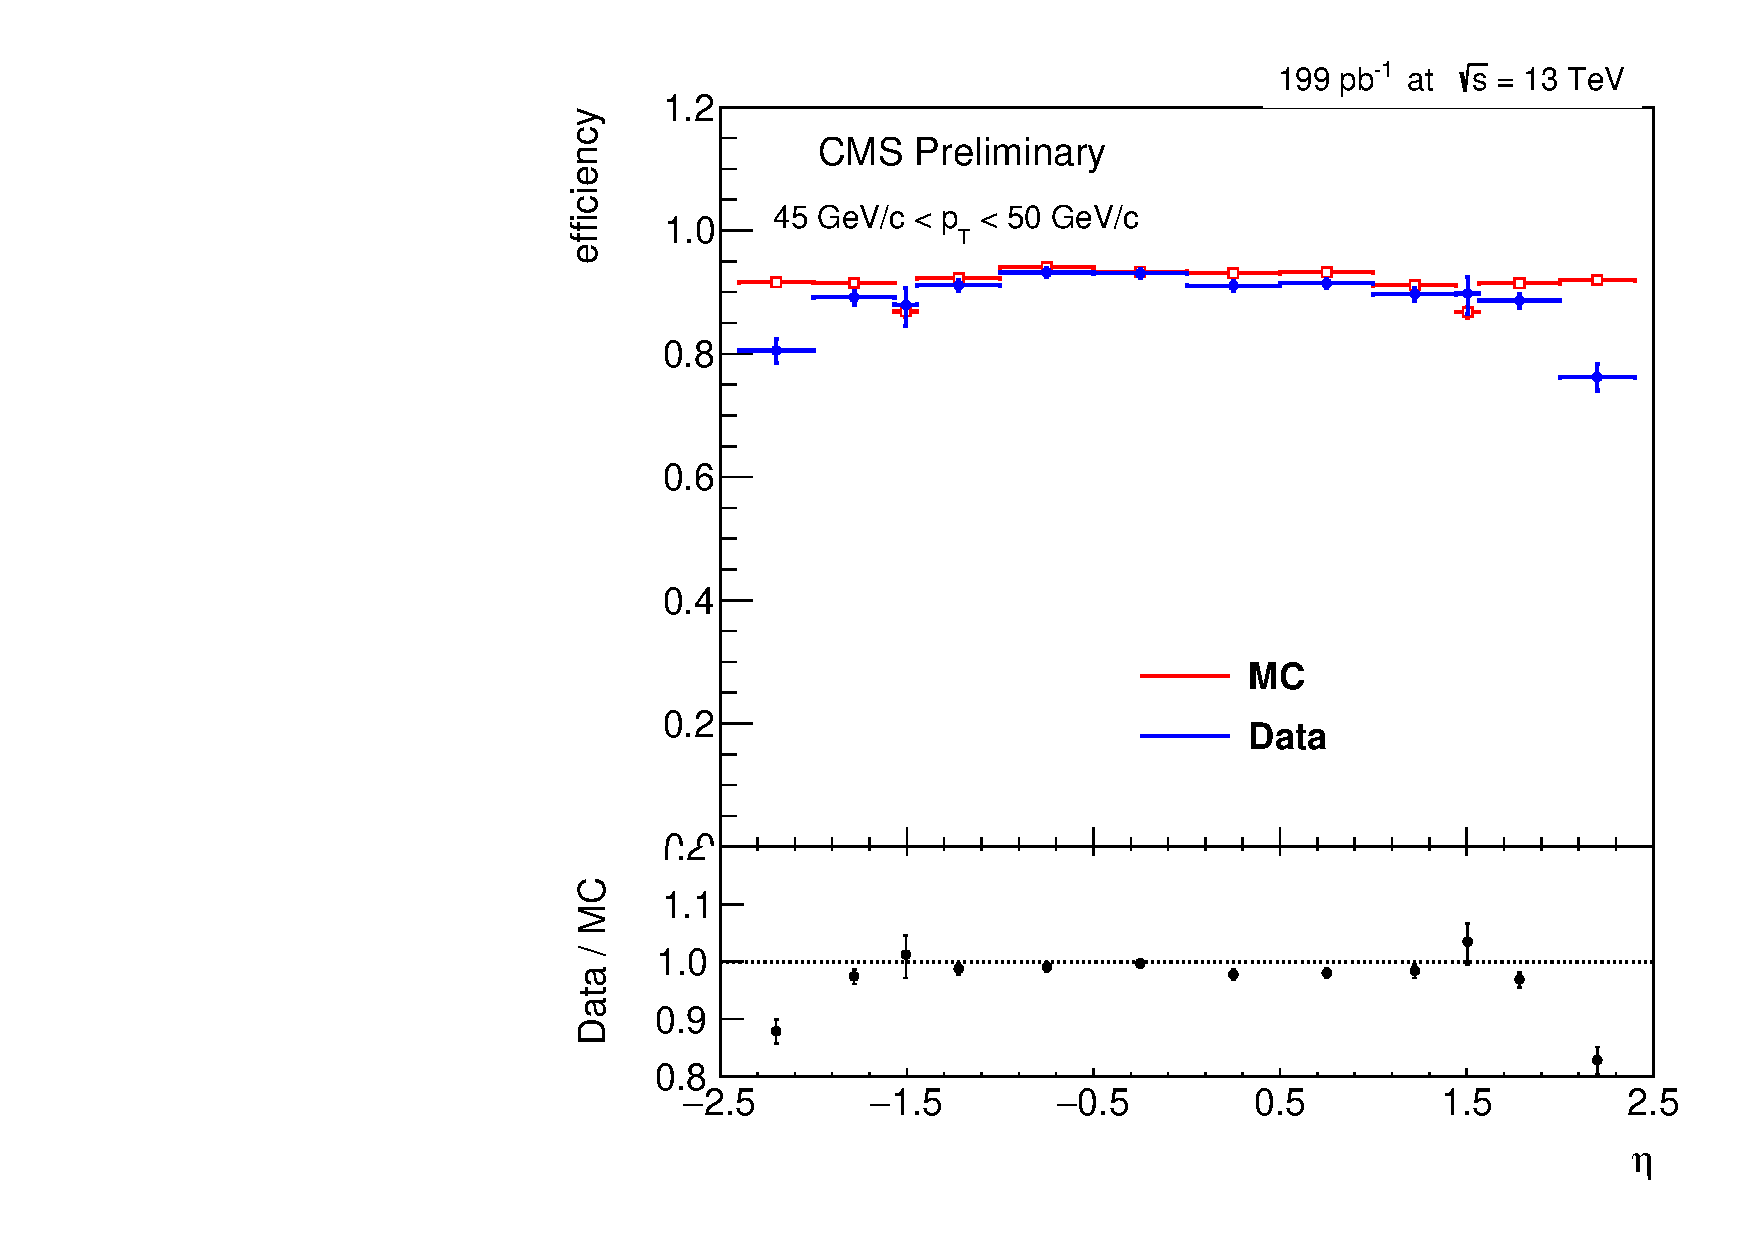
\includegraphics[width=0.45\linewidth]{plots/efficiency/13_zeehlt_negative/PtBins_eta_pt8.pdf}
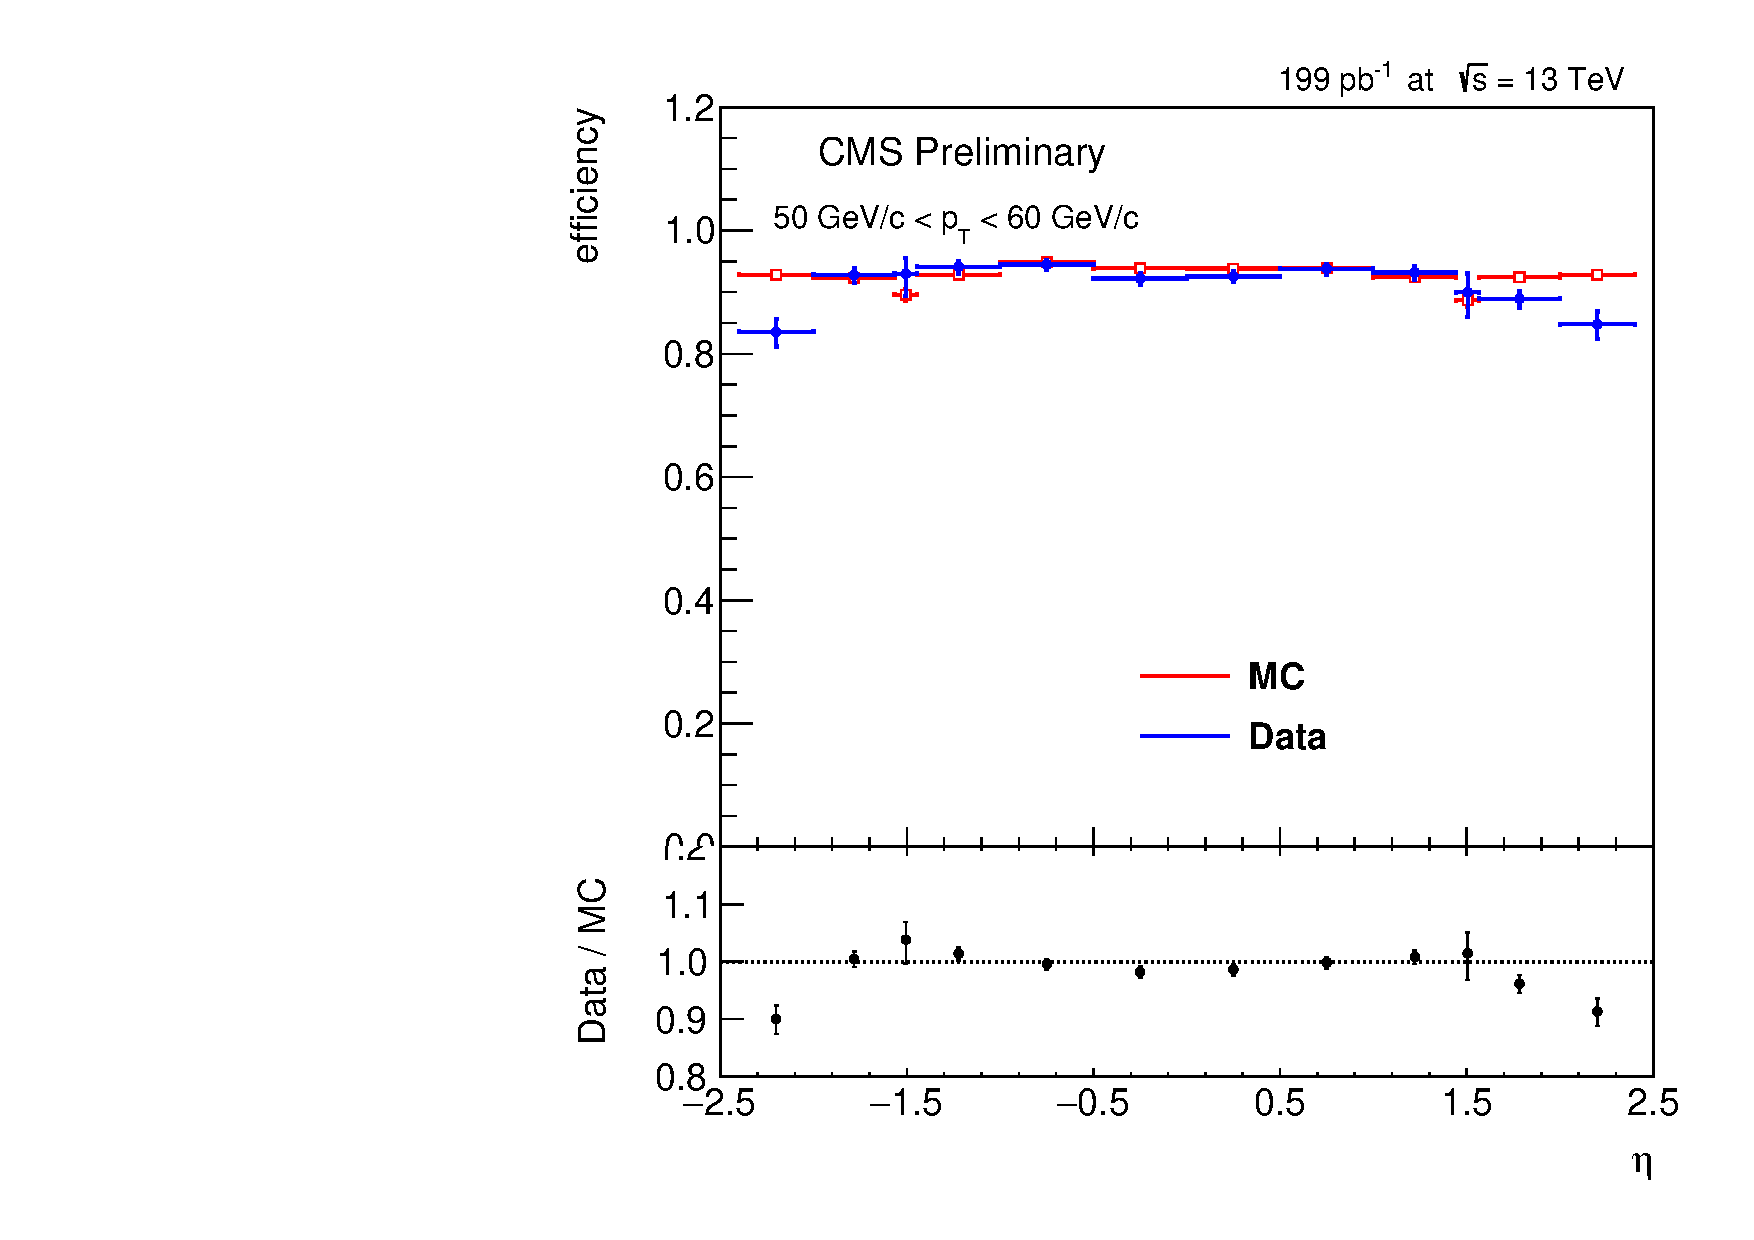
\includegraphics[width=0.45\linewidth]{plots/efficiency/13_zeehlt_negative/PtBins_eta_pt9.pdf}
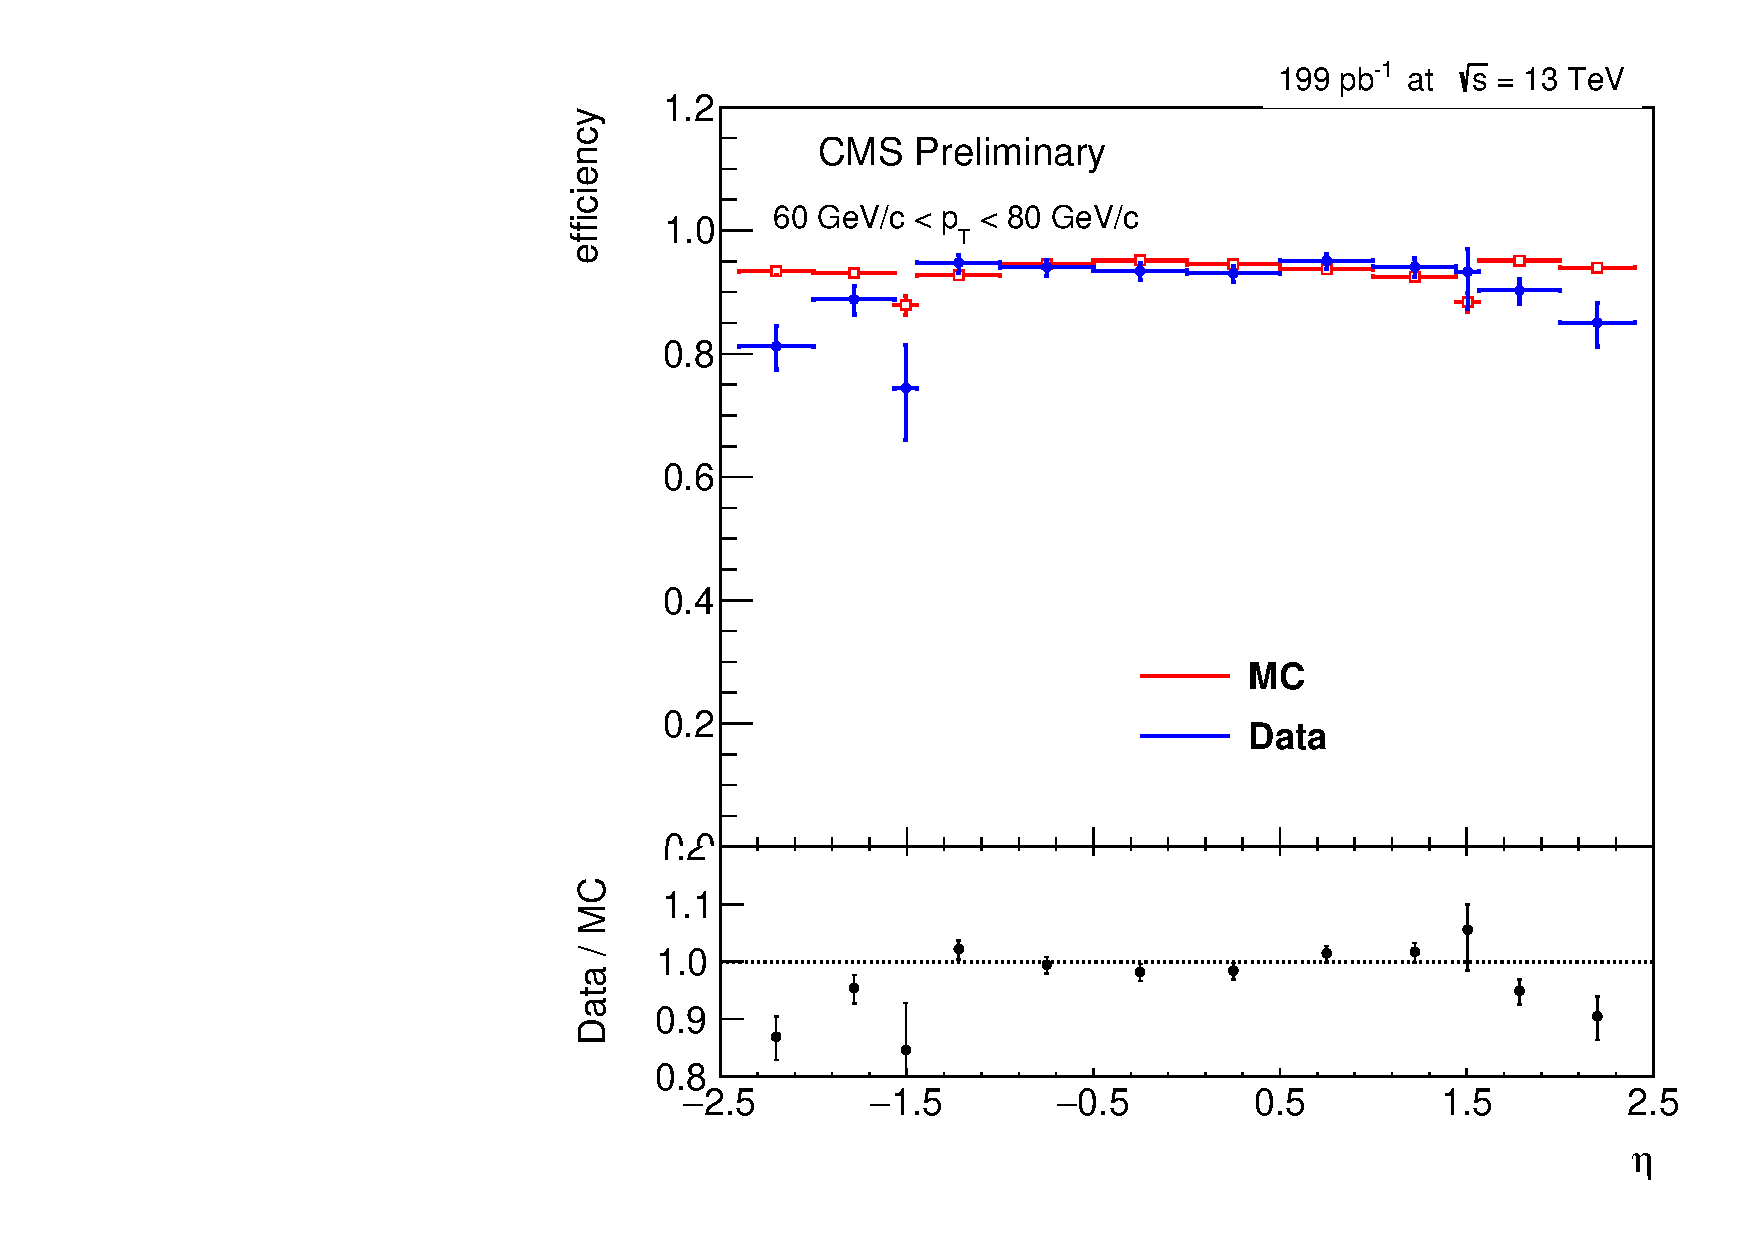
\includegraphics[width=0.45\linewidth]{plots/efficiency/13_zeehlt_negative/PtBins_eta_pt10.pdf}
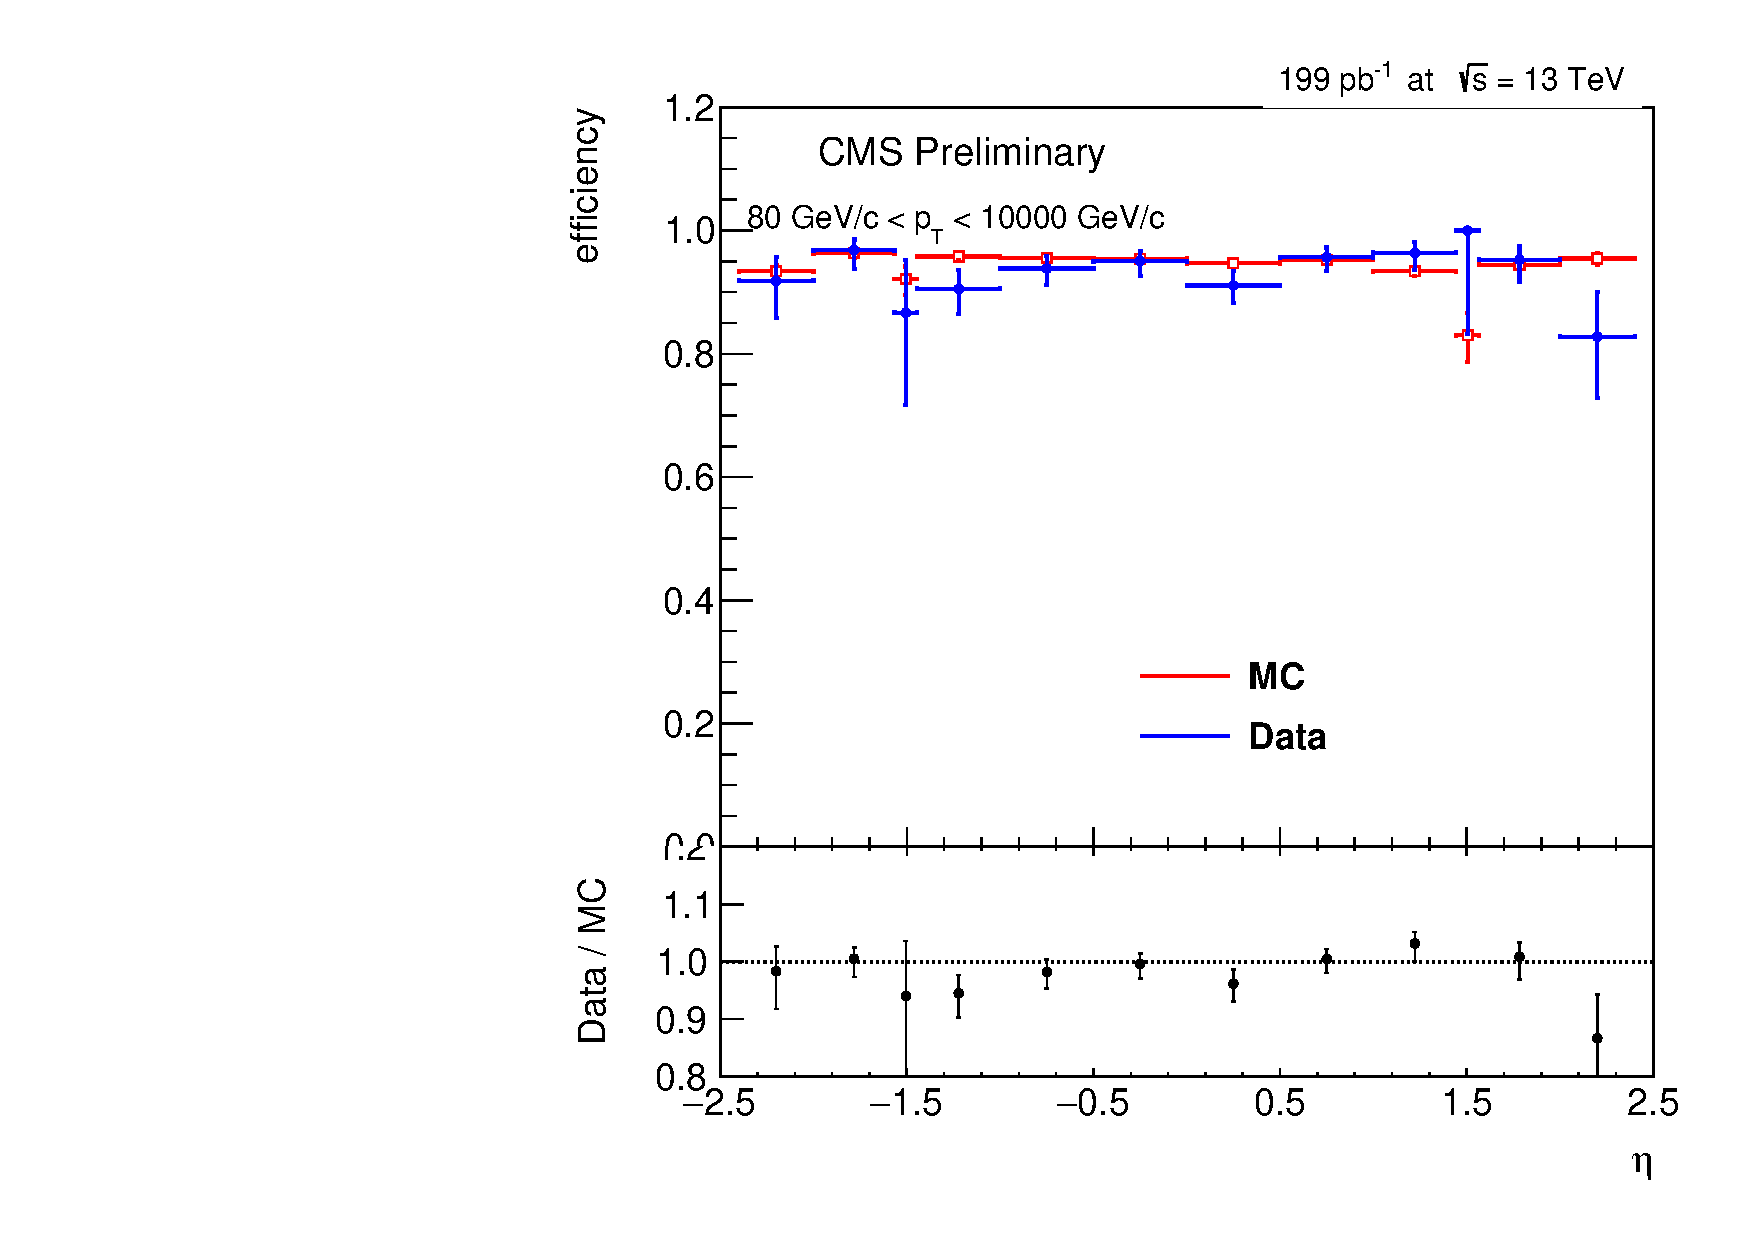
\includegraphics[width=0.45\linewidth]{plots/efficiency/13_zeehlt_negative/PtBins_eta_pt11.pdf}
\caption{$\eta$ dependence of Single electron trigger efficiency scale factors, separated by $p_T$ bins, for negatively charged electrons in the 13 TeV samples.}
\label{fig:Eff:el:13:HLT:neg}
\end{figure}


%%%% Figures for MuSIT Efficiency  %%%%%
\begin{figure}
\centering
\includegraphics[width=0.32\linewidth]{plots/efficiency/13_zmmsit_combined/PtBins_eta_pt0.pdf}
\includegraphics[width=0.32\linewidth]{plots/efficiency/13_zmmsit_combined/PtBins_eta_pt1.pdf}
\includegraphics[width=0.32\linewidth]{plots/efficiency/13_zmmsit_combined/PtBins_eta_pt2.pdf}
\caption{$\eta$ dependence of Muon selection efficiency scale factors, separated by $p_T$ bins, for combined charged muons in the 13 TeV samples.}
\label{fig:Eff:mu:13:SIT:com}
\end{figure}

%%%% Figures for MuSta Efficiency  %%%%%
\begin{figure}
\centering
\includegraphics[width=0.32\linewidth]{plots/efficiency/13_zmmsta_combined/PtBins_eta_pt0.pdf}
\includegraphics[width=0.32\linewidth]{plots/efficiency/13_zmmsta_combined/PtBins_eta_pt1.pdf}
\includegraphics[width=0.32\linewidth]{plots/efficiency/13_zmmsta_combined/PtBins_eta_pt2.pdf}
\caption{$\eta$ dependence of Standalone muon identification efficiency scale factors, separated by $p_T$ bins, for combined charged muons in the 13 TeV samples.}
\label{fig:Eff:mu:13:Sta:com}
\end{figure}

%%%% Figures for MuHLT Efficiency  %%%%%
\begin{figure}
\centering
\includegraphics[width=0.32\linewidth]{plots/efficiency/13_zmmhlt_positive/PtBins_eta_pt0.pdf}
\includegraphics[width=0.32\linewidth]{plots/efficiency/13_zmmhlt_positive/PtBins_eta_pt1.pdf}
\includegraphics[width=0.32\linewidth]{plots/efficiency/13_zmmhlt_positive/PtBins_eta_pt10.pdf}
\includegraphics[width=0.32\linewidth]{plots/efficiency/13_zmmhlt_positive/PtBins_eta_pt11.pdf}
\includegraphics[width=0.32\linewidth]{plots/efficiency/13_zmmhlt_positive/PtBins_eta_pt2.pdf}
\includegraphics[width=0.32\linewidth]{plots/efficiency/13_zmmhlt_positive/PtBins_eta_pt3.pdf}
\includegraphics[width=0.32\linewidth]{plots/efficiency/13_zmmhlt_positive/PtBins_eta_pt4.pdf}
\includegraphics[width=0.32\linewidth]{plots/efficiency/13_zmmhlt_positive/PtBins_eta_pt5.pdf}
\includegraphics[width=0.32\linewidth]{plots/efficiency/13_zmmhlt_positive/PtBins_eta_pt6.pdf}
\includegraphics[width=0.32\linewidth]{plots/efficiency/13_zmmhlt_positive/PtBins_eta_pt7.pdf}
\includegraphics[width=0.32\linewidth]{plots/efficiency/13_zmmhlt_positive/PtBins_eta_pt8.pdf}
\includegraphics[width=0.32\linewidth]{plots/efficiency/13_zmmhlt_positive/PtBins_eta_pt9.pdf}
\caption{$\eta$ dependence of Single muon trigger efficiency scale factors, separated by $p_T$ bins, for positively charged muons in the 13 TeV samples.}
\label{fig:Eff:mu:13:HLT:pos}
\end{figure}
\begin{figure}
\centering
\includegraphics[width=0.32\linewidth]{plots/efficiency/13_zmmhlt_negative/PtBins_eta_pt0.pdf}
\includegraphics[width=0.32\linewidth]{plots/efficiency/13_zmmhlt_negative/PtBins_eta_pt1.pdf}
\includegraphics[width=0.32\linewidth]{plots/efficiency/13_zmmhlt_negative/PtBins_eta_pt10.pdf}
\includegraphics[width=0.32\linewidth]{plots/efficiency/13_zmmhlt_negative/PtBins_eta_pt11.pdf}
\includegraphics[width=0.32\linewidth]{plots/efficiency/13_zmmhlt_negative/PtBins_eta_pt2.pdf}
\includegraphics[width=0.32\linewidth]{plots/efficiency/13_zmmhlt_negative/PtBins_eta_pt3.pdf}
\includegraphics[width=0.32\linewidth]{plots/efficiency/13_zmmhlt_negative/PtBins_eta_pt4.pdf}
\includegraphics[width=0.32\linewidth]{plots/efficiency/13_zmmhlt_negative/PtBins_eta_pt5.pdf}
\includegraphics[width=0.32\linewidth]{plots/efficiency/13_zmmhlt_negative/PtBins_eta_pt6.pdf}
\includegraphics[width=0.32\linewidth]{plots/efficiency/13_zmmhlt_negative/PtBins_eta_pt7.pdf}
\includegraphics[width=0.32\linewidth]{plots/efficiency/13_zmmhlt_negative/PtBins_eta_pt8.pdf}
\includegraphics[width=0.32\linewidth]{plots/efficiency/13_zmmhlt_negative/PtBins_eta_pt9.pdf}
\caption{$\eta$ dependence of Single muon trigger efficiency scale factors, separated by $p_T$ bins, for negatively charged muons in the 13 TeV samples.}
\label{fig:Eff:mu:13:HLT:neg}
\end{figure}


%%%% Tables for EleGSFSel Efficiency  %%%%%
%% Efficiency table for ZeeGSFSel Combined
\begin{table}%[htbp]
\begin{center}
\scalebox{0.6}{
\begin{tabular}{ccccccc}
\hline
& $-2.4< \eta<-2$ & $-2< \eta<-1.566$ & $-1.566< \eta<-1.4442$ & $-1.4442< \eta<-1$ & $-1< \eta<-0.5$ & $-0.5< \eta<0$ \\
\hline \hline
$25<p_{T}<35$ & $0.959 \pm 0.018$ & $0.904 \pm 0.009$ & $0.885 \pm 0.052$ & $0.863 \pm 0.018$ & $0.855 \pm 0.013$ & $0.872 \pm 0.007$  \\
$35<p_{T}<50$ & $0.969 \pm 0.009$ & $0.934 \pm 0.009$ & $0.896 \pm 0.015$ & $0.904 \pm 0.005$ & $0.908 \pm 0.003$ & $0.905 \pm 0.004$  \\
$50<p_{T}<1e+04$ & $0.955 \pm 0.017$ & $0.971 \pm 0.014$ & $1.014 \pm 0.037$ & $0.921 \pm 0.012$ & $0.925 \pm 0.008$ & $0.899 \pm 0.007$  \\
\hline
& $0< \eta<0.5$ & $0.5< \eta<1$ & $1< \eta<1.44$ & $1.44< \eta<1.57$ & $1.57< \eta<2$ & $2< \eta<2.4$ \\
\hline \hline
$25<p_{T}<35$ & $0.891 \pm 0.013$ & $0.902 \pm 0.013$ & $0.844 \pm 0.015$ & $0.943 \pm 0.045$ & $0.925 \pm 0.010$ & $0.922 \pm 0.020$  \\
$35<p_{T}<50$ & $0.917 \pm 0.005$ & $0.936 \pm 0.001$ & $0.941 \pm 0.001$ & $0.923 \pm 0.021$ & $0.948 \pm 0.007$ & $0.954 \pm 0.006$  \\
$50<p_{T}<1e+04$ & $0.919 \pm 0.009$ & $0.943 \pm 0.009$ & $0.956 \pm 0.012$ & $0.959 \pm 0.089$ & $0.949 \pm 0.054$ & $0.982 \pm 0.020$  \\
\hline
\end{tabular}}
\end{center}
\caption{GSF electron identification and isolation efficiency scale factors in ($p_T$, $\eta$) bins for combined charged electrons in the 13 TeV samples.}
\label{tab:Eff:el:13TeV:GSFSel:com}
\end{table}

%%%% Tables for EleHLT Efficiency  %%%%%
%% Efficiency table for ZeeHLT Positive
\begin{table}%[htbp]
\begin{center}
\scalebox{0.6}{
\begin{tabular}{ccccccc}
\hline
& $-2.4< \eta<-2$ & $-2< \eta<-1.566$ & $-1.566< \eta<-1.4442$ & $-1.4442< \eta<-1$ & $-1< \eta<-0.5$ & $-0.5< \eta<0$ \\
\hline \hline
$25<p_{T}<26.5$ & $0.664 \pm 0.058$ & $0.921 \pm 0.054$ & $0.959 \pm 0.112$ & $1.053 \pm 0.046$ & $0.964 \pm 0.036$ & $1.031 \pm 0.030$  \\
$26.5<p_{T}<28$ & $0.646 \pm 0.056$ & $0.928 \pm 0.043$ & $1.033 \pm 0.103$ & $0.976 \pm 0.041$ & $0.962 \pm 0.031$ & $0.933 \pm 0.032$  \\
$28<p_{T}<29.5$ & $0.754 \pm 0.055$ & $0.986 \pm 0.037$ & $1.004 \pm 0.101$ & $1.016 \pm 0.037$ & $0.948 \pm 0.030$ & $0.977 \pm 0.025$  \\
$29.5<p_{T}<31$ & $0.624 \pm 0.048$ & $0.959 \pm 0.034$ & $0.981 \pm 0.093$ & $0.990 \pm 0.034$ & $0.961 \pm 0.027$ & $0.987 \pm 0.022$  \\
$31<p_{T}<32.5$ & $0.725 \pm 0.042$ & $0.907 \pm 0.036$ & $0.942 \pm 0.078$ & $1.037 \pm 0.028$ & $0.996 \pm 0.020$ & $0.991 \pm 0.020$  \\
$32.5<p_{T}<35$ & $0.747 \pm 0.032$ & $0.959 \pm 0.023$ & $0.972 \pm 0.065$ & $0.976 \pm 0.022$ & $0.979 \pm 0.014$ & $0.971 \pm 0.014$  \\
$35<p_{T}<40$ & $0.811 \pm 0.020$ & $0.957 \pm 0.014$ & $0.987 \pm 0.038$ & $0.995 \pm 0.011$ & $0.982 \pm 0.008$ & $0.991 \pm 0.008$  \\
$40<p_{T}<45$ & $0.831 \pm 0.018$ & $0.986 \pm 0.011$ & $0.976 \pm 0.029$ & $0.996 \pm 0.009$ & $0.999 \pm 0.006$ & $0.978 \pm 0.007$  \\
$45<p_{T}<50$ & $0.875 \pm 0.020$ & $0.966 \pm 0.013$ & $1.030 \pm 0.033$ & $0.985 \pm 0.011$ & $0.984 \pm 0.008$ & $0.980 \pm 0.008$  \\
$50<p_{T}<60$ & $0.857 \pm 0.026$ & $0.986 \pm 0.015$ & $0.988 \pm 0.048$ & $1.008 \pm 0.012$ & $0.989 \pm 0.009$ & $0.988 \pm 0.010$  \\
$60<p_{T}<80$ & $0.889 \pm 0.035$ & $0.998 \pm 0.024$ & $1.051 \pm 0.056$ & $0.993 \pm 0.018$ & $0.992 \pm 0.014$ & $0.974 \pm 0.016$  \\
$80<p_{T}<1e+04$ & $1.033 \pm 0.039$ & $0.978 \pm 0.036$ & $1.009 \pm 0.105$ & $0.996 \pm 0.027$ & $0.976 \pm 0.025$ & $0.980 \pm 0.026$  \\
\hline
& $0< \eta<0.5$ & $0.5< \eta<1$ & $1< \eta<1.44$ & $1.44< \eta<1.57$ & $1.57< \eta<2$ & $2< \eta<2.4$ \\
\hline \hline
$25<p_{T}<26.5$ & $0.952 \pm 0.035$ & $0.940 \pm 0.036$ & $1.088 \pm 0.039$ & $1.052 \pm 0.134$ & $0.871 \pm 0.048$ & $0.658 \pm 0.067$  \\
$26.5<p_{T}<28$ & $1.005 \pm 0.030$ & $0.958 \pm 0.033$ & $0.989 \pm 0.043$ & $1.082 \pm 0.131$ & $0.898 \pm 0.044$ & $0.800 \pm 0.059$  \\
$28<p_{T}<29.5$ & $0.980 \pm 0.026$ & $0.995 \pm 0.026$ & $0.964 \pm 0.046$ & $0.872 \pm 0.126$ & $0.968 \pm 0.039$ & $0.622 \pm 0.056$  \\
$29.5<p_{T}<31$ & $0.992 \pm 0.021$ & $0.964 \pm 0.025$ & $0.939 \pm 0.040$ & $1.000 \pm 0.105$ & $0.935 \pm 0.036$ & $0.751 \pm 0.049$  \\
$31<p_{T}<32.5$ & $0.980 \pm 0.020$ & $0.976 \pm 0.021$ & $1.025 \pm 0.029$ & $1.010 \pm 0.085$ & $0.923 \pm 0.035$ & $0.666 \pm 0.053$  \\
$32.5<p_{T}<35$ & $0.976 \pm 0.014$ & $0.970 \pm 0.014$ & $1.016 \pm 0.021$ & $0.807 \pm 0.083$ & $0.946 \pm 0.023$ & $0.805 \pm 0.032$  \\
$35<p_{T}<40$ & $0.972 \pm 0.008$ & $0.976 \pm 0.008$ & $0.993 \pm 0.011$ & $0.975 \pm 0.037$ & $0.963 \pm 0.014$ & $0.814 \pm 0.021$  \\
$40<p_{T}<45$ & $0.978 \pm 0.007$ & $0.987 \pm 0.007$ & $0.991 \pm 0.009$ & $1.022 \pm 0.031$ & $0.974 \pm 0.011$ & $0.846 \pm 0.019$  \\
$45<p_{T}<50$ & $0.973 \pm 0.008$ & $0.986 \pm 0.008$ & $0.997 \pm 0.011$ & $0.963 \pm 0.040$ & $0.952 \pm 0.013$ & $0.866 \pm 0.022$  \\
$50<p_{T}<60$ & $0.998 \pm 0.009$ & $0.980 \pm 0.010$ & $1.019 \pm 0.012$ & $0.995 \pm 0.043$ & $0.968 \pm 0.016$ & $0.907 \pm 0.026$  \\
$60<p_{T}<80$ & $0.970 \pm 0.017$ & $0.987 \pm 0.014$ & $1.016 \pm 0.017$ & $0.937 \pm 0.074$ & $0.989 \pm 0.023$ & $0.956 \pm 0.035$  \\
$80<p_{T}<1e+04$ & $0.982 \pm 0.022$ & $0.978 \pm 0.027$ & $1.048 \pm 0.017$ & $1.096 \pm 0.082$ & $0.950 \pm 0.043$ & $0.967 \pm 0.055$  \\
\hline
\end{tabular}}
\end{center}
\caption{Single electron trigger efficiency scale factors in ($p_T$, $\eta$) bins for positively charged electrons in the 13 TeV samples.}
\label{tab:Eff:el:13TeV:HLT:pos}
\end{table}
%% Efficiency table for ZeeHLT Negative
\begin{table}%[htbp]
\begin{center}
\scalebox{0.6}{
\begin{tabular}{ccccccc}
\hline
& $-2.4< \eta<-2$ & $-2< \eta<-1.566$ & $-1.566< \eta<-1.4442$ & $-1.4442< \eta<-1$ & $-1< \eta<-0.5$ & $-0.5< \eta<0$ \\
\hline \hline
$25<p_{T}<26.5$ & $0.722 \pm 0.059$ & $0.895 \pm 0.053$ & $0.909 \pm 0.133$ & $0.992 \pm 0.050$ & $0.965 \pm 0.034$ & $0.996 \pm 0.032$  \\
$26.5<p_{T}<28$ & $0.736 \pm 0.060$ & $0.922 \pm 0.047$ & $0.920 \pm 0.141$ & $1.002 \pm 0.040$ & $1.005 \pm 0.029$ & $0.963 \pm 0.028$  \\
$28<p_{T}<29.5$ & $0.746 \pm 0.052$ & $0.897 \pm 0.043$ & $0.965 \pm 0.117$ & $1.034 \pm 0.031$ & $0.971 \pm 0.027$ & $0.972 \pm 0.025$  \\
$29.5<p_{T}<31$ & $0.716 \pm 0.049$ & $0.953 \pm 0.033$ & $0.890 \pm 0.095$ & $0.994 \pm 0.030$ & $0.970 \pm 0.024$ & $0.971 \pm 0.022$  \\
$31<p_{T}<32.5$ & $0.745 \pm 0.044$ & $0.921 \pm 0.034$ & $1.023 \pm 0.107$ & $1.060 \pm 0.026$ & $1.006 \pm 0.020$ & $0.980 \pm 0.021$  \\
$32.5<p_{T}<35$ & $0.814 \pm 0.033$ & $0.977 \pm 0.024$ & $0.989 \pm 0.062$ & $1.001 \pm 0.018$ & $0.984 \pm 0.014$ & $0.972 \pm 0.015$  \\
$35<p_{T}<40$ & $0.768 \pm 0.020$ & $0.955 \pm 0.014$ & $0.989 \pm 0.039$ & $0.978 \pm 0.012$ & $0.985 \pm 0.007$ & $0.968 \pm 0.008$  \\
$40<p_{T}<45$ & $0.826 \pm 0.018$ & $0.977 \pm 0.011$ & $0.940 \pm 0.038$ & $1.003 \pm 0.009$ & $0.986 \pm 0.007$ & $0.984 \pm 0.007$  \\
$45<p_{T}<50$ & $0.879 \pm 0.021$ & $0.974 \pm 0.012$ & $1.012 \pm 0.037$ & $0.988 \pm 0.011$ & $0.991 \pm 0.008$ & $0.997 \pm 0.008$  \\
$50<p_{T}<60$ & $0.900 \pm 0.025$ & $1.005 \pm 0.014$ & $1.038 \pm 0.037$ & $1.014 \pm 0.011$ & $0.996 \pm 0.009$ & $0.982 \pm 0.010$  \\
$60<p_{T}<80$ & $0.869 \pm 0.038$ & $0.954 \pm 0.025$ & $0.846 \pm 0.089$ & $1.022 \pm 0.017$ & $0.995 \pm 0.014$ & $0.982 \pm 0.015$  \\
$80<p_{T}<1e+04$ & $0.983 \pm 0.055$ & $1.005 \pm 0.026$ & $0.941 \pm 0.134$ & $0.945 \pm 0.038$ & $0.982 \pm 0.025$ & $0.996 \pm 0.022$  \\
\hline
& $0< \eta<0.5$ & $0.5< \eta<1$ & $1< \eta<1.44$ & $1.44< \eta<1.57$ & $1.57< \eta<2$ & $2< \eta<2.4$ \\
\hline \hline
$25<p_{T}<26.5$ & $0.955 \pm 0.037$ & $0.969 \pm 0.035$ & $0.967 \pm 0.050$ & $0.999 \pm 0.136$ & $0.911 \pm 0.050$ & $0.703 \pm 0.068$  \\
$26.5<p_{T}<28$ & $0.971 \pm 0.031$ & $1.033 \pm 0.033$ & $1.010 \pm 0.043$ & $0.958 \pm 0.118$ & $0.902 \pm 0.044$ & $0.673 \pm 0.059$  \\
$28<p_{T}<29.5$ & $0.973 \pm 0.026$ & $0.987 \pm 0.025$ & $1.020 \pm 0.038$ & $0.994 \pm 0.102$ & $0.978 \pm 0.038$ & $0.815 \pm 0.053$  \\
$29.5<p_{T}<31$ & $0.945 \pm 0.025$ & $0.946 \pm 0.027$ & $1.020 \pm 0.034$ & $0.978 \pm 0.121$ & $0.886 \pm 0.037$ & $0.701 \pm 0.055$  \\
$31<p_{T}<32.5$ & $0.999 \pm 0.021$ & $0.979 \pm 0.021$ & $1.015 \pm 0.033$ & $0.927 \pm 0.110$ & $0.982 \pm 0.032$ & $0.781 \pm 0.048$  \\
$32.5<p_{T}<35$ & $0.963 \pm 0.015$ & $0.992 \pm 0.015$ & $1.014 \pm 0.020$ & $1.008 \pm 0.061$ & $0.973 \pm 0.021$ & $0.764 \pm 0.033$  \\
$35<p_{T}<40$ & $0.975 \pm 0.008$ & $0.975 \pm 0.008$ & $1.002 \pm 0.011$ & $0.963 \pm 0.039$ & $0.957 \pm 0.013$ & $0.824 \pm 0.021$  \\
$40<p_{T}<45$ & $0.983 \pm 0.007$ & $0.979 \pm 0.007$ & $0.989 \pm 0.009$ & $1.019 \pm 0.029$ & $0.964 \pm 0.011$ & $0.864 \pm 0.018$  \\
$45<p_{T}<50$ & $0.978 \pm 0.008$ & $0.980 \pm 0.008$ & $0.984 \pm 0.012$ & $1.035 \pm 0.036$ & $0.969 \pm 0.013$ & $0.829 \pm 0.023$  \\
$50<p_{T}<60$ & $0.986 \pm 0.010$ & $0.999 \pm 0.010$ & $1.008 \pm 0.012$ & $1.015 \pm 0.042$ & $0.962 \pm 0.016$ & $0.913 \pm 0.024$  \\
$60<p_{T}<80$ & $0.984 \pm 0.014$ & $1.015 \pm 0.014$ & $1.017 \pm 0.017$ & $1.056 \pm 0.059$ & $0.949 \pm 0.022$ & $0.905 \pm 0.038$  \\
$80<p_{T}<1e+04$ & $0.962 \pm 0.028$ & $1.005 \pm 0.021$ & $1.032 \pm 0.026$ & $1.204 \pm 0.154$ & $1.008 \pm 0.033$ & $0.867 \pm 0.092$  \\
\hline
\end{tabular}}
\end{center}
\caption{Single electron trigger efficiency scale factors in ($p_T$, $\eta$) bins for negatively charged electrons in the 13 TeV samples.}
\label{tab:Eff:el:13TeV:HLT:neg}
\end{table}


%%%% Tables for MuSIT Efficiency  %%%%%
%% Efficiency table for ZmmSIT Combined
\begin{table}%[htbp]
\begin{center}
\scalebox{0.6}{
\begin{tabular}{ccccccc}
\hline
& $-2.4< \eta<-2.1$ & $-2.1< \eta<-1.6$ & $-1.6< \eta<-1.2$ & $-1.2< \eta<-0.9$ & $-0.9< \eta<-0.3$ & $-0.3< \eta<0$ \\
\hline \hline
$25<p_{T}<35$ & $0.993 \pm 0.006$ & $1.009 \pm 0.005$ & $0.998 \pm 0.006$ & $1.002 \pm 0.007$ & $0.993 \pm 0.004$ & $0.985 \pm 0.005$  \\
$35<p_{T}<50$ & $0.987 \pm 0.003$ & $0.996 \pm 0.002$ & $0.998 \pm 0.002$ & $0.990 \pm 0.002$ & $0.993 \pm 0.002$ & $0.988 \pm 0.002$  \\
$50<p_{T}<1e+04$ & $0.975 \pm 0.007$ & $0.992 \pm 0.007$ & $0.997 \pm 0.003$ & $0.992 \pm 0.005$ & $0.993 \pm 0.003$ & $0.992 \pm 0.005$  \\
\hline
& $0< \eta<0.3$ & $0.3< \eta<0.9$ & $0.9< \eta<1.2$ & $1.2< \eta<1.6$ & $1.6< \eta<2.1$ & $2.1< \eta<2.4$ \\
\hline \hline
$25<p_{T}<35$ & $0.989 \pm 0.006$ & $0.992 \pm 0.004$ & $0.984 \pm 0.007$ & $0.999 \pm 0.006$ & $1.005 \pm 0.005$ & $1.003 \pm 0.006$  \\
$35<p_{T}<50$ & $0.995 \pm 0.003$ & $0.992 \pm 0.002$ & $0.988 \pm 0.002$ & $0.997 \pm 0.002$ & $1.002 \pm 0.001$ & $0.994 \pm 0.002$  \\
$50<p_{T}<1e+04$ & $0.979 \pm 0.005$ & $0.992 \pm 0.003$ & $0.994 \pm 0.005$ & $0.987 \pm 0.003$ & $0.997 \pm 0.003$ & $0.989 \pm 0.006$  \\
\hline
\end{tabular}}
\end{center}
\caption{Muon selection efficiency scale factors in ($p_T$, $\eta$) bins for combined charged muons in the 13 TeV samples.}
\label{tab:Eff:mu:13TeV:SIT:com}
\end{table}

%%%% Tables for MuSta Efficiency  %%%%%
%% Efficiency table for ZmmSta Combined
\begin{table}%[htbp]
\begin{center}
\scalebox{0.6}{
\begin{tabular}{ccccccc}
\hline
& $-2.4< \eta<-2.1$ & $-2.1< \eta<-1.6$ & $-1.6< \eta<-1.2$ & $-1.2< \eta<-0.9$ & $-0.9< \eta<-0.3$ & $-0.3< \eta<0$ \\
\hline \hline
$25<p_{T}<35$ & $0.990 \pm 0.007$ & $0.991 \pm 0.004$ & $0.986 \pm 0.006$ & $0.997 \pm 0.034$ & $0.992 \pm 0.009$ & $0.991 \pm 0.014$  \\
$35<p_{T}<50$ & $0.994 \pm 0.002$ & $0.996 \pm 0.002$ & $0.998 \pm 0.002$ & $0.997 \pm 0.002$ & $0.998 \pm 0.001$ & $0.986 \pm 0.002$  \\
$50<p_{T}<1e+04$ & $0.996 \pm 0.013$ & $0.995 \pm 0.004$ & $0.995 \pm 0.004$ & $0.995 \pm 0.005$ & $0.997 \pm 0.003$ & $0.989 \pm 0.005$  \\
\hline
& $0< \eta<0.3$ & $0.3< \eta<0.9$ & $0.9< \eta<1.2$ & $1.2< \eta<1.6$ & $1.6< \eta<2.1$ & $2.1< \eta<2.4$ \\
\hline \hline
$25<p_{T}<35$ & $0.983 \pm 0.006$ & $0.988 \pm 0.014$ & $1.008 \pm 0.017$ & $1.009 \pm 0.005$ & $1.004 \pm 0.008$ & $0.994 \pm 0.001$  \\
$35<p_{T}<50$ & $0.988 \pm 0.002$ & $0.991 \pm 0.002$ & $0.995 \pm 0.000$ & $0.998 \pm 0.002$ & $0.998 \pm 0.002$ & $0.996 \pm 0.001$  \\
$50<p_{T}<1e+04$ & $0.981 \pm 0.005$ & $0.988 \pm 0.003$ & $0.995 \pm 0.004$ & $0.995 \pm 0.004$ & $0.997 \pm 0.003$ & $0.992 \pm 0.005$  \\
\hline
\end{tabular}}
\end{center}
\caption{Standalone muon identification efficiency scale factors in ($p_T$, $\eta$) bins for combined charged muons in the 13 TeV samples.}
\label{tab:Eff:mu:13TeV:Sta:com}
\end{table}

%%%% Tables for MuHLT Efficiency  %%%%%
%% Efficiency table for ZmmHLT Positive
\begin{table}%[htbp]
\begin{center}
\scalebox{0.6}{
\begin{tabular}{ccccccc}
\hline
& $-2.4< \eta<-2.1$ & $-2.1< \eta<-1.6$ & $-1.6< \eta<-1.2$ & $-1.2< \eta<-0.9$ & $-0.9< \eta<-0.3$ & $-0.3< \eta<0$ \\
\hline \hline
$25<p_{T}<26.5$ & $0.960 \pm 0.030$ & $0.999 \pm 0.017$ & $0.928 \pm 0.023$ & $0.984 \pm 0.021$ & $0.981 \pm 0.012$ & $0.981 \pm 0.017$  \\
$26.5<p_{T}<28$ & $0.984 \pm 0.023$ & $0.984 \pm 0.016$ & $0.967 \pm 0.016$ & $0.978 \pm 0.019$ & $0.988 \pm 0.011$ & $0.976 \pm 0.016$  \\
$28<p_{T}<29.5$ & $0.974 \pm 0.023$ & $0.965 \pm 0.017$ & $0.987 \pm 0.014$ & $0.987 \pm 0.015$ & $0.987 \pm 0.010$ & $0.985 \pm 0.013$  \\
$29.5<p_{T}<31$ & $0.946 \pm 0.025$ & $0.971 \pm 0.015$ & $0.975 \pm 0.015$ & $0.973 \pm 0.016$ & $0.977 \pm 0.010$ & $1.013 \pm 0.010$  \\
$31<p_{T}<32.5$ & $0.974 \pm 0.020$ & $0.993 \pm 0.013$ & $0.964 \pm 0.014$ & $0.979 \pm 0.015$ & $0.986 \pm 0.008$ & $0.980 \pm 0.013$  \\
$32.5<p_{T}<35$ & $0.979 \pm 0.014$ & $0.969 \pm 0.011$ & $0.967 \pm 0.011$ & $0.984 \pm 0.009$ & $0.993 \pm 0.006$ & $0.982 \pm 0.009$  \\
$35<p_{T}<40$ & $0.988 \pm 0.009$ & $0.978 \pm 0.006$ & $0.963 \pm 0.006$ & $0.973 \pm 0.006$ & $0.986 \pm 0.004$ & $0.991 \pm 0.005$  \\
$40<p_{T}<45$ & $0.970 \pm 0.009$ & $0.972 \pm 0.006$ & $0.963 \pm 0.005$ & $0.972 \pm 0.005$ & $0.986 \pm 0.003$ & $0.990 \pm 0.005$  \\
$45<p_{T}<50$ & $0.947 \pm 0.012$ & $0.980 \pm 0.006$ & $0.968 \pm 0.006$ & $0.967 \pm 0.007$ & $0.986 \pm 0.004$ & $0.989 \pm 0.007$  \\
$50<p_{T}<60$ & $0.971 \pm 0.014$ & $0.984 \pm 0.009$ & $0.976 \pm 0.007$ & $0.971 \pm 0.008$ & $0.972 \pm 0.006$ & $0.992 \pm 0.009$  \\
$60<p_{T}<80$ & $1.004 \pm 0.023$ & $0.979 \pm 0.014$ & $0.962 \pm 0.013$ & $0.973 \pm 0.014$ & $0.988 \pm 0.009$ & $0.983 \pm 0.013$  \\
$80<p_{T}<1e+04$ & $0.951 \pm 0.082$ & $1.010 \pm 0.026$ & $0.949 \pm 0.026$ & $0.901 \pm 0.034$ & $0.953 \pm 0.020$ & $0.966 \pm 0.025$  \\
\hline
& $0< \eta<0.3$ & $0.3< \eta<0.9$ & $0.9< \eta<1.2$ & $1.2< \eta<1.6$ & $1.6< \eta<2.1$ & $2.1< \eta<2.4$ \\
\hline \hline
$25<p_{T}<26.5$ & $0.955 \pm 0.020$ & $0.981 \pm 0.012$ & $0.979 \pm 0.020$ & $0.960 \pm 0.020$ & $1.007 \pm 0.011$ & $0.993 \pm 0.023$  \\
$26.5<p_{T}<28$ & $1.004 \pm 0.014$ & $0.963 \pm 0.012$ & $0.958 \pm 0.021$ & $0.944 \pm 0.021$ & $1.001 \pm 0.012$ & $0.988 \pm 0.023$  \\
$28<p_{T}<29.5$ & $0.997 \pm 0.013$ & $0.966 \pm 0.011$ & $0.984 \pm 0.014$ & $0.987 \pm 0.015$ & $0.985 \pm 0.012$ & $0.972 \pm 0.021$  \\
$29.5<p_{T}<31$ & $0.979 \pm 0.013$ & $0.964 \pm 0.010$ & $0.939 \pm 0.019$ & $0.972 \pm 0.016$ & $0.984 \pm 0.011$ & $0.992 \pm 0.017$  \\
$31<p_{T}<32.5$ & $0.969 \pm 0.013$ & $0.969 \pm 0.009$ & $0.959 \pm 0.016$ & $0.961 \pm 0.015$ & $0.990 \pm 0.010$ & $1.001 \pm 0.017$  \\
$32.5<p_{T}<35$ & $0.987 \pm 0.009$ & $0.970 \pm 0.006$ & $0.957 \pm 0.012$ & $0.988 \pm 0.009$ & $0.983 \pm 0.008$ & $0.987 \pm 0.013$  \\
$35<p_{T}<40$ & $0.982 \pm 0.006$ & $0.967 \pm 0.004$ & $0.961 \pm 0.006$ & $0.968 \pm 0.006$ & $0.982 \pm 0.005$ & $0.998 \pm 0.007$  \\
$40<p_{T}<45$ & $0.979 \pm 0.005$ & $0.976 \pm 0.003$ & $0.972 \pm 0.005$ & $0.972 \pm 0.005$ & $0.985 \pm 0.004$ & $0.985 \pm 0.007$  \\
$45<p_{T}<50$ & $0.971 \pm 0.007$ & $0.968 \pm 0.005$ & $0.957 \pm 0.007$ & $0.976 \pm 0.006$ & $0.986 \pm 0.005$ & $0.981 \pm 0.010$  \\
$50<p_{T}<60$ & $0.979 \pm 0.009$ & $0.955 \pm 0.006$ & $0.969 \pm 0.009$ & $0.968 \pm 0.008$ & $0.996 \pm 0.005$ & $0.968 \pm 0.012$  \\
$60<p_{T}<80$ & $0.957 \pm 0.015$ & $0.978 \pm 0.008$ & $0.940 \pm 0.016$ & $0.998 \pm 0.010$ & $0.993 \pm 0.009$ & $0.969 \pm 0.023$  \\
$80<p_{T}<1e+04$ & $0.990 \pm 0.024$ & $0.974 \pm 0.017$ & $0.924 \pm 0.032$ & $0.948 \pm 0.027$ & $0.996 \pm 0.020$ & $0.960 \pm 0.048$  \\
\hline
\end{tabular}}
\end{center}
\caption{Single muon trigger efficiency scale factors in ($p_T$, $\eta$) bins for positively charged muons in the 13 TeV samples.}
\label{tab:Eff:mu:13TeV:HLT:pos}
\end{table}
%% Efficiency table for ZmmHLT Negative
\begin{table}%[htbp]
\begin{center}
\scalebox{0.6}{
\begin{tabular}{ccccccc}
\hline
& $-2.4< \eta<-2.1$ & $-2.1< \eta<-1.6$ & $-1.6< \eta<-1.2$ & $-1.2< \eta<-0.9$ & $-0.9< \eta<-0.3$ & $-0.3< \eta<0$ \\
\hline \hline
$25<p_{T}<26.5$ & $0.990 \pm 0.024$ & $0.975 \pm 0.019$ & $0.968 \pm 0.020$ & $0.975 \pm 0.022$ & $0.997 \pm 0.010$ & $1.002 \pm 0.016$  \\
$26.5<p_{T}<28$ & $0.983 \pm 0.023$ & $0.962 \pm 0.019$ & $0.944 \pm 0.020$ & $0.981 \pm 0.018$ & $0.969 \pm 0.011$ & $0.968 \pm 0.017$  \\
$28<p_{T}<29.5$ & $1.016 \pm 0.021$ & $0.968 \pm 0.017$ & $0.957 \pm 0.018$ & $0.966 \pm 0.017$ & $0.963 \pm 0.010$ & $1.004 \pm 0.011$  \\
$29.5<p_{T}<31$ & $0.968 \pm 0.022$ & $0.980 \pm 0.015$ & $0.966 \pm 0.015$ & $0.979 \pm 0.016$ & $0.980 \pm 0.008$ & $0.989 \pm 0.012$  \\
$31<p_{T}<32.5$ & $0.981 \pm 0.021$ & $0.994 \pm 0.013$ & $0.958 \pm 0.014$ & $0.980 \pm 0.013$ & $0.976 \pm 0.008$ & $0.994 \pm 0.011$  \\
$32.5<p_{T}<35$ & $0.947 \pm 0.016$ & $0.968 \pm 0.011$ & $0.965 \pm 0.011$ & $0.972 \pm 0.010$ & $0.988 \pm 0.005$ & $0.993 \pm 0.008$  \\
$35<p_{T}<40$ & $0.969 \pm 0.010$ & $0.973 \pm 0.006$ & $0.968 \pm 0.006$ & $0.975 \pm 0.006$ & $0.987 \pm 0.003$ & $0.989 \pm 0.005$  \\
$40<p_{T}<45$ & $0.971 \pm 0.009$ & $0.976 \pm 0.006$ & $0.970 \pm 0.005$ & $0.976 \pm 0.005$ & $0.981 \pm 0.003$ & $0.987 \pm 0.005$  \\
$45<p_{T}<50$ & $0.962 \pm 0.012$ & $0.977 \pm 0.007$ & $0.972 \pm 0.006$ & $0.978 \pm 0.006$ & $0.986 \pm 0.004$ & $0.991 \pm 0.006$  \\
$50<p_{T}<60$ & $0.957 \pm 0.015$ & $0.965 \pm 0.009$ & $0.972 \pm 0.008$ & $0.980 \pm 0.008$ & $0.975 \pm 0.006$ & $0.971 \pm 0.009$  \\
$60<p_{T}<80$ & $0.941 \pm 0.025$ & $0.956 \pm 0.015$ & $0.982 \pm 0.011$ & $0.969 \pm 0.014$ & $1.000 \pm 0.007$ & $1.006 \pm 0.011$  \\
$80<p_{T}<1e+04$ & $0.940 \pm 0.057$ & $0.965 \pm 0.028$ & $0.917 \pm 0.031$ & $0.957 \pm 0.028$ & $0.965 \pm 0.016$ & $0.986 \pm 0.026$  \\
\hline
& $0< \eta<0.3$ & $0.3< \eta<0.9$ & $0.9< \eta<1.2$ & $1.2< \eta<1.6$ & $1.6< \eta<2.1$ & $2.1< \eta<2.4$ \\
\hline \hline
$25<p_{T}<26.5$ & $0.986 \pm 0.015$ & $0.994 \pm 0.009$ & $0.991 \pm 0.020$ & $0.966 \pm 0.020$ & $0.997 \pm 0.012$ & $1.002 \pm 0.017$  \\
$26.5<p_{T}<28$ & $0.986 \pm 0.014$ & $0.986 \pm 0.010$ & $0.967 \pm 0.020$ & $0.951 \pm 0.021$ & $0.987 \pm 0.013$ & $0.994 \pm 0.023$  \\
$28<p_{T}<29.5$ & $0.966 \pm 0.015$ & $0.993 \pm 0.010$ & $0.993 \pm 0.014$ & $0.938 \pm 0.020$ & $0.997 \pm 0.010$ & $0.996 \pm 0.020$  \\
$29.5<p_{T}<31$ & $0.967 \pm 0.015$ & $0.986 \pm 0.009$ & $0.989 \pm 0.014$ & $0.961 \pm 0.017$ & $0.995 \pm 0.010$ & $0.993 \pm 0.017$  \\
$31<p_{T}<32.5$ & $0.992 \pm 0.012$ & $0.982 \pm 0.008$ & $0.972 \pm 0.014$ & $0.927 \pm 0.018$ & $0.990 \pm 0.010$ & $1.004 \pm 0.016$  \\
$32.5<p_{T}<35$ & $0.985 \pm 0.008$ & $0.993 \pm 0.005$ & $0.969 \pm 0.010$ & $0.964 \pm 0.010$ & $0.991 \pm 0.007$ & $0.992 \pm 0.012$  \\
$35<p_{T}<40$ & $0.978 \pm 0.006$ & $0.973 \pm 0.004$ & $0.969 \pm 0.006$ & $0.965 \pm 0.006$ & $0.994 \pm 0.004$ & $0.995 \pm 0.007$  \\
$40<p_{T}<45$ & $0.983 \pm 0.005$ & $0.981 \pm 0.003$ & $0.965 \pm 0.006$ & $0.974 \pm 0.005$ & $0.991 \pm 0.004$ & $0.985 \pm 0.007$  \\
$45<p_{T}<50$ & $0.981 \pm 0.007$ & $0.975 \pm 0.005$ & $0.957 \pm 0.008$ & $0.971 \pm 0.006$ & $0.988 \pm 0.005$ & $0.977 \pm 0.009$  \\
$50<p_{T}<60$ & $0.983 \pm 0.009$ & $0.974 \pm 0.006$ & $0.971 \pm 0.009$ & $0.975 \pm 0.008$ & $0.994 \pm 0.006$ & $0.990 \pm 0.012$  \\
$60<p_{T}<80$ & $1.003 \pm 0.013$ & $0.980 \pm 0.009$ & $0.942 \pm 0.016$ & $0.984 \pm 0.011$ & $0.995 \pm 0.009$ & $0.954 \pm 0.023$  \\
$80<p_{T}<1e+04$ & $0.944 \pm 0.031$ & $0.962 \pm 0.018$ & $0.981 \pm 0.023$ & $0.993 \pm 0.021$ & $1.001 \pm 0.019$ & $1.024 \pm 0.038$  \\
\hline
\end{tabular}}
\end{center}
\caption{Single muon trigger efficiency scale factors in ($p_T$, $\eta$) bins for negatively charged muons in the 13 TeV samples.}
\label{tab:Eff:mu:13TeV:HLT:neg}
\end{table}


%%%% Figures for EleGSFSel Efficiency  %%%%%
\begin{figure}
\centering
\includegraphics[width=0.32\linewidth]{plots/efficiency/5_zeegsfsel_combined/PtBins_eta_pt0.pdf}
\includegraphics[width=0.32\linewidth]{plots/efficiency/5_zeegsfsel_combined/PtBins_eta_pt1.pdf}
\includegraphics[width=0.32\linewidth]{plots/efficiency/5_zeegsfsel_combined/PtBins_eta_pt2.pdf}
\caption{$\eta$ dependence of GSF electron identification and isolation efficiency scale factors, separated by $p_T$ bins, for combined charged electrons in the 5 TeV samples.}
\label{fig:Eff:el:5:GSFSel:com}
\end{figure}

%%%% Figures for EleHLT Efficiency  %%%%%
\begin{figure}
\centering
\includegraphics[width=0.32\linewidth]{plots/efficiency/5_zeehlt_positive/PtBins_eta_pt0.pdf}
\includegraphics[width=0.32\linewidth]{plots/efficiency/5_zeehlt_positive/PtBins_eta_pt1.pdf}
\includegraphics[width=0.32\linewidth]{plots/efficiency/5_zeehlt_positive/PtBins_eta_pt10.pdf}
\includegraphics[width=0.32\linewidth]{plots/efficiency/5_zeehlt_positive/PtBins_eta_pt11.pdf}
\includegraphics[width=0.32\linewidth]{plots/efficiency/5_zeehlt_positive/PtBins_eta_pt2.pdf}
\includegraphics[width=0.32\linewidth]{plots/efficiency/5_zeehlt_positive/PtBins_eta_pt3.pdf}
\includegraphics[width=0.32\linewidth]{plots/efficiency/5_zeehlt_positive/PtBins_eta_pt4.pdf}
\includegraphics[width=0.32\linewidth]{plots/efficiency/5_zeehlt_positive/PtBins_eta_pt5.pdf}
\includegraphics[width=0.32\linewidth]{plots/efficiency/5_zeehlt_positive/PtBins_eta_pt6.pdf}
\includegraphics[width=0.32\linewidth]{plots/efficiency/5_zeehlt_positive/PtBins_eta_pt7.pdf}
\includegraphics[width=0.32\linewidth]{plots/efficiency/5_zeehlt_positive/PtBins_eta_pt8.pdf}
\includegraphics[width=0.32\linewidth]{plots/efficiency/5_zeehlt_positive/PtBins_eta_pt9.pdf}
\caption{$\eta$ dependence of Single electron trigger efficiency scale factors, separated by $p_T$ bins, for positively charged electrons in the 5 TeV samples.}
\label{fig:Eff:el:5:HLT:pos}
\end{figure}
\begin{figure}
\centering
\includegraphics[width=0.32\linewidth]{plots/efficiency/5_zeehlt_negative/PtBins_eta_pt0.pdf}
\includegraphics[width=0.32\linewidth]{plots/efficiency/5_zeehlt_negative/PtBins_eta_pt1.pdf}
\includegraphics[width=0.32\linewidth]{plots/efficiency/5_zeehlt_negative/PtBins_eta_pt10.pdf}
\includegraphics[width=0.32\linewidth]{plots/efficiency/5_zeehlt_negative/PtBins_eta_pt11.pdf}
\includegraphics[width=0.32\linewidth]{plots/efficiency/5_zeehlt_negative/PtBins_eta_pt2.pdf}
\includegraphics[width=0.32\linewidth]{plots/efficiency/5_zeehlt_negative/PtBins_eta_pt3.pdf}
\includegraphics[width=0.32\linewidth]{plots/efficiency/5_zeehlt_negative/PtBins_eta_pt4.pdf}
\includegraphics[width=0.32\linewidth]{plots/efficiency/5_zeehlt_negative/PtBins_eta_pt5.pdf}
\includegraphics[width=0.32\linewidth]{plots/efficiency/5_zeehlt_negative/PtBins_eta_pt6.pdf}
\includegraphics[width=0.32\linewidth]{plots/efficiency/5_zeehlt_negative/PtBins_eta_pt7.pdf}
\includegraphics[width=0.32\linewidth]{plots/efficiency/5_zeehlt_negative/PtBins_eta_pt8.pdf}
\includegraphics[width=0.32\linewidth]{plots/efficiency/5_zeehlt_negative/PtBins_eta_pt9.pdf}
\caption{$\eta$ dependence of Single electron trigger efficiency scale factors, separated by $p_T$ bins, for negatively charged electrons in the 5 TeV samples.}
\label{fig:Eff:el:5:HLT:neg}
\end{figure}


%%%% Figures for MuSIT Efficiency  %%%%%
\begin{figure}
\centering
\includegraphics[width=0.32\linewidth]{plots/efficiency/5_zmmsit_combined/PtBins_eta_pt0.pdf}
\includegraphics[width=0.32\linewidth]{plots/efficiency/5_zmmsit_combined/PtBins_eta_pt1.pdf}
\includegraphics[width=0.32\linewidth]{plots/efficiency/5_zmmsit_combined/PtBins_eta_pt2.pdf}
\caption{$\eta$ dependence of Muon selection efficiency scale factors, separated by $p_T$ bins, for combined charged muons in the 5 TeV samples.}
\label{fig:Eff:mu:5:SIT:com}
\end{figure}

%%%% Figures for MuSta Efficiency  %%%%%
\begin{figure}
\centering
\includegraphics[width=0.48\linewidth]{plots/efficiency/5_zmmsta_combined/PtBins_eta_pt0.pdf}
\includegraphics[width=0.48\linewidth]{plots/efficiency/5_zmmsta_combined/PtBins_eta_pt1.pdf}
\includegraphics[width=0.48\linewidth]{plots/efficiency/5_zmmsta_combined/PtBins_eta_pt2.pdf}
\caption{$\eta$ dependence of Standalone muon identification efficiency scale factors, separated by $p_T$ bins, for combined charged muons in the 5 TeV samples.}
\label{fig:Eff:mu:5:Sta:com}
\end{figure}

%%%% Figures for MuHLT Efficiency  %%%%%
\begin{figure}
\centering
\includegraphics[width=0.32\linewidth]{plots/efficiency/5_zmmhlt_positive/PtBins_eta_pt0.pdf}
\includegraphics[width=0.32\linewidth]{plots/efficiency/5_zmmhlt_positive/PtBins_eta_pt1.pdf}
\includegraphics[width=0.32\linewidth]{plots/efficiency/5_zmmhlt_positive/PtBins_eta_pt10.pdf}
\includegraphics[width=0.32\linewidth]{plots/efficiency/5_zmmhlt_positive/PtBins_eta_pt11.pdf}
\includegraphics[width=0.32\linewidth]{plots/efficiency/5_zmmhlt_positive/PtBins_eta_pt2.pdf}
\includegraphics[width=0.32\linewidth]{plots/efficiency/5_zmmhlt_positive/PtBins_eta_pt3.pdf}
\includegraphics[width=0.32\linewidth]{plots/efficiency/5_zmmhlt_positive/PtBins_eta_pt4.pdf}
\includegraphics[width=0.32\linewidth]{plots/efficiency/5_zmmhlt_positive/PtBins_eta_pt5.pdf}
\includegraphics[width=0.32\linewidth]{plots/efficiency/5_zmmhlt_positive/PtBins_eta_pt6.pdf}
\includegraphics[width=0.32\linewidth]{plots/efficiency/5_zmmhlt_positive/PtBins_eta_pt7.pdf}
\includegraphics[width=0.32\linewidth]{plots/efficiency/5_zmmhlt_positive/PtBins_eta_pt8.pdf}
\includegraphics[width=0.32\linewidth]{plots/efficiency/5_zmmhlt_positive/PtBins_eta_pt9.pdf}
\caption{$\eta$ dependence of Single muon trigger efficiency scale factors, separated by $p_T$ bins, for positively charged muons in the 5 TeV samples.}
\label{fig:Eff:mu:5:HLT:pos}
\end{figure}
\begin{figure}
\centering
\includegraphics[width=0.32\linewidth]{plots/efficiency/5_zmmhlt_negative/PtBins_eta_pt0.pdf}
\includegraphics[width=0.32\linewidth]{plots/efficiency/5_zmmhlt_negative/PtBins_eta_pt1.pdf}
\includegraphics[width=0.32\linewidth]{plots/efficiency/5_zmmhlt_negative/PtBins_eta_pt10.pdf}
\includegraphics[width=0.32\linewidth]{plots/efficiency/5_zmmhlt_negative/PtBins_eta_pt11.pdf}
\includegraphics[width=0.32\linewidth]{plots/efficiency/5_zmmhlt_negative/PtBins_eta_pt2.pdf}
\includegraphics[width=0.32\linewidth]{plots/efficiency/5_zmmhlt_negative/PtBins_eta_pt3.pdf}
\includegraphics[width=0.32\linewidth]{plots/efficiency/5_zmmhlt_negative/PtBins_eta_pt4.pdf}
\includegraphics[width=0.32\linewidth]{plots/efficiency/5_zmmhlt_negative/PtBins_eta_pt5.pdf}
\includegraphics[width=0.32\linewidth]{plots/efficiency/5_zmmhlt_negative/PtBins_eta_pt6.pdf}
\includegraphics[width=0.32\linewidth]{plots/efficiency/5_zmmhlt_negative/PtBins_eta_pt7.pdf}
\includegraphics[width=0.32\linewidth]{plots/efficiency/5_zmmhlt_negative/PtBins_eta_pt8.pdf}
\includegraphics[width=0.32\linewidth]{plots/efficiency/5_zmmhlt_negative/PtBins_eta_pt9.pdf}
\caption{$\eta$ dependence of Single muon trigger efficiency scale factors, separated by $p_T$ bins, for negatively charged muons in the 5 TeV samples.}
\label{fig:Eff:mu:5:HLT:neg}
\end{figure}


%%%% Tables for EleGSFSel Efficiency  %%%%%
%% Efficiency table for ZeeGSFSel Combined
\begin{table}%[htbp]
\begin{center}
\scalebox{0.6}{
\begin{tabular}{ccccccc}
\hline
& $-2.4< \eta<-2$ & $-2< \eta<-1.566$ & $-1.566< \eta<-1.4442$ & $-1.4442< \eta<-1$ & $-1< \eta<-0.5$ & $-0.5< \eta<0$ \\
\hline \hline
$25<p_{T}<35$ & $0.982 \pm 0.021$ & $0.911 \pm 0.012$ & $1.022 \pm 0.093$ & $0.905 \pm 0.023$ & $0.936 \pm 0.016$ & $0.947 \pm 0.011$  \\
$35<p_{T}<50$ & $0.974 \pm 0.010$ & $0.948 \pm 0.006$ & $0.939 \pm 0.020$ & $0.939 \pm 0.005$ & $0.947 \pm 0.005$ & $0.934 \pm 0.005$  \\
$50<p_{T}<1e+04$ & $0.981 \pm 0.021$ & $0.971 \pm 0.019$ & $0.991 \pm 0.043$ & $0.944 \pm 0.010$ & $0.958 \pm 0.011$ & $0.971 \pm 0.013$  \\
\hline
& $0< \eta<0.5$ & $0.5< \eta<1$ & $1< \eta<1.44$ & $1.44< \eta<1.57$ & $1.57< \eta<2$ & $2< \eta<2.4$ \\
\hline \hline
$25<p_{T}<35$ & $0.910 \pm 0.014$ & $0.925 \pm 0.017$ & $0.886 \pm 0.019$ & $0.873 \pm 0.043$ & $0.867 \pm 0.003$ & $0.966 \pm 0.023$  \\
$35<p_{T}<50$ & $0.934 \pm 0.004$ & $0.938 \pm 0.005$ & $0.925 \pm 0.008$ & $0.992 \pm 0.029$ & $0.945 \pm 0.006$ & $0.932 \pm 0.010$  \\
$50<p_{T}<1e+04$ & $0.932 \pm 0.008$ & $0.964 \pm 0.012$ & $0.955 \pm 0.010$ & $1.015 \pm 0.061$ & $0.953 \pm 0.017$ & $0.979 \pm 0.022$  \\
\hline
\end{tabular}}
\end{center}
\caption{GSF electron identification and isolation efficiency scale factors in ($p_T$, $\eta$) bins for combined charged electrons in the 5 TeV samples.}
\label{tab:Eff:el:5TeV:GSFSel:com}
\end{table}

%%%% Tables for EleHLT Efficiency  %%%%%
%% Efficiency table for ZeeHLT Positive
\begin{table}%[htbp]
\begin{center}
\scalebox{0.6}{
\begin{tabular}{ccccccc}
\hline
& $-2.4< \eta<-2$ & $-2< \eta<-1.566$ & $-1.566< \eta<-1.4442$ & $-1.4442< \eta<-1$ & $-1< \eta<-0.5$ & $-0.5< \eta<0$ \\
\hline \hline
$25<p_{T}<26.5$ & $0.530 \pm 0.086$ & $0.851 \pm 0.064$ & $0.713 \pm 0.266$ & $1.038 \pm 0.063$ & $0.969 \pm 0.050$ & $0.930 \pm 0.049$  \\
$26.5<p_{T}<28$ & $0.629 \pm 0.077$ & $0.903 \pm 0.059$ & $0.721 \pm 0.184$ & $1.051 \pm 0.053$ & $0.955 \pm 0.044$ & $0.959 \pm 0.042$  \\
$28<p_{T}<29.5$ & $0.641 \pm 0.067$ & $0.915 \pm 0.055$ & $1.103 \pm 0.127$ & $1.018 \pm 0.048$ & $0.926 \pm 0.041$ & $0.971 \pm 0.033$  \\
$29.5<p_{T}<31$ & $0.603 \pm 0.066$ & $0.917 \pm 0.047$ & $0.893 \pm 0.143$ & $0.980 \pm 0.041$ & $0.948 \pm 0.032$ & $0.946 \pm 0.032$  \\
$31<p_{T}<32.5$ & $0.700 \pm 0.063$ & $0.927 \pm 0.047$ & $0.886 \pm 0.129$ & $0.949 \pm 0.045$ & $0.956 \pm 0.027$ & $0.969 \pm 0.028$  \\
$32.5<p_{T}<35$ & $0.686 \pm 0.044$ & $0.913 \pm 0.032$ & $0.862 \pm 0.102$ & $0.951 \pm 0.029$ & $0.927 \pm 0.021$ & $0.962 \pm 0.019$  \\
$35<p_{T}<40$ & $0.817 \pm 0.025$ & $0.934 \pm 0.018$ & $0.931 \pm 0.051$ & $0.960 \pm 0.015$ & $0.935 \pm 0.012$ & $0.965 \pm 0.011$  \\
$40<p_{T}<45$ & $0.818 \pm 0.023$ & $0.933 \pm 0.015$ & $0.968 \pm 0.037$ & $0.970 \pm 0.012$ & $0.955 \pm 0.010$ & $0.964 \pm 0.009$  \\
$45<p_{T}<50$ & $0.827 \pm 0.029$ & $0.942 \pm 0.018$ & $0.984 \pm 0.049$ & $0.988 \pm 0.013$ & $0.964 \pm 0.012$ & $0.953 \pm 0.012$  \\
$50<p_{T}<60$ & $0.868 \pm 0.036$ & $0.895 \pm 0.027$ & $0.999 \pm 0.066$ & $1.005 \pm 0.018$ & $0.941 \pm 0.017$ & $0.969 \pm 0.015$  \\
$60<p_{T}<80$ & $0.890 \pm 0.082$ & $0.955 \pm 0.040$ & $0.931 \pm 0.143$ & $0.993 \pm 0.027$ & $0.972 \pm 0.026$ & $0.967 \pm 0.028$  \\
$80<p_{T}<1e+04$ & $0.952 \pm 0.225$ & $0.987 \pm 0.066$ & $0.833 \pm 0.449$ & $1.030 \pm 0.055$ & $0.983 \pm 0.041$ & $0.924 \pm 0.070$  \\
\hline
& $0< \eta<0.5$ & $0.5< \eta<1$ & $1< \eta<1.44$ & $1.44< \eta<1.57$ & $1.57< \eta<2$ & $2< \eta<2.4$ \\
\hline \hline
$25<p_{T}<26.5$ & $0.885 \pm 0.051$ & $0.901 \pm 0.054$ & $1.099 \pm 0.056$ & $0.890 \pm 0.192$ & $0.814 \pm 0.074$ & $0.641 \pm 0.087$  \\
$26.5<p_{T}<28$ & $0.938 \pm 0.047$ & $0.951 \pm 0.044$ & $1.008 \pm 0.059$ & $0.872 \pm 0.165$ & $0.808 \pm 0.068$ & $0.666 \pm 0.080$  \\
$28<p_{T}<29.5$ & $0.984 \pm 0.032$ & $0.962 \pm 0.042$ & $0.961 \pm 0.057$ & $0.860 \pm 0.168$ & $0.846 \pm 0.057$ & $0.692 \pm 0.090$  \\
$29.5<p_{T}<31$ & $0.964 \pm 0.034$ & $0.977 \pm 0.033$ & $0.976 \pm 0.046$ & $1.220 \pm 0.320$ & $0.906 \pm 0.052$ & $0.724 \pm 0.074$  \\
$31<p_{T}<32.5$ & $0.955 \pm 0.028$ & $0.947 \pm 0.033$ & $0.952 \pm 0.045$ & $0.801 \pm 0.118$ & $0.897 \pm 0.049$ & $0.743 \pm 0.077$  \\
$32.5<p_{T}<35$ & $0.929 \pm 0.020$ & $0.934 \pm 0.021$ & $0.916 \pm 0.034$ & $0.954 \pm 0.096$ & $0.853 \pm 0.037$ & $0.699 \pm 0.048$  \\
$35<p_{T}<40$ & $0.969 \pm 0.011$ & $0.955 \pm 0.011$ & $0.958 \pm 0.016$ & $0.937 \pm 0.050$ & $0.916 \pm 0.019$ & $0.764 \pm 0.029$  \\
$40<p_{T}<45$ & $0.954 \pm 0.010$ & $0.951 \pm 0.010$ & $0.945 \pm 0.014$ & $0.946 \pm 0.045$ & $0.937 \pm 0.016$ & $0.796 \pm 0.026$  \\
$45<p_{T}<50$ & $0.954 \pm 0.012$ & $0.954 \pm 0.013$ & $0.990 \pm 0.015$ & $0.948 \pm 0.051$ & $0.893 \pm 0.021$ & $0.829 \pm 0.031$  \\
$50<p_{T}<60$ & $0.948 \pm 0.018$ & $0.956 \pm 0.017$ & $0.932 \pm 0.023$ & $0.996 \pm 0.066$ & $0.984 \pm 0.023$ & $0.947 \pm 0.037$  \\
$60<p_{T}<80$ & $0.943 \pm 0.029$ & $0.942 \pm 0.032$ & $1.013 \pm 0.027$ & $1.016 \pm 0.143$ & $1.021 \pm 0.037$ & $1.020 \pm 0.062$  \\
$80<p_{T}<1e+04$ & $0.888 \pm 0.063$ & $0.960 \pm 0.057$ & $1.055 \pm 0.061$ & $0.576 \pm 0.365$ & $0.979 \pm 0.078$ & $0.882 \pm 0.240$  \\
\hline
\end{tabular}}
\end{center}
\caption{Single electron trigger efficiency scale factors in ($p_T$, $\eta$) bins for positively charged electrons in the 5 TeV samples.}
\label{tab:Eff:el:5TeV:HLT:pos}
\end{table}
%% Efficiency table for ZeeHLT Negative
\begin{table}%[htbp]
\begin{center}
\scalebox{0.6}{
\begin{tabular}{ccccccc}
\hline
& $-2.4< \eta<-2$ & $-2< \eta<-1.566$ & $-1.566< \eta<-1.4442$ & $-1.4442< \eta<-1$ & $-1< \eta<-0.5$ & $-0.5< \eta<0$ \\
\hline \hline
$25<p_{T}<26.5$ & $0.771 \pm 0.079$ & $0.887 \pm 0.065$ & $1.130 \pm 0.178$ & $1.056 \pm 0.062$ & $0.948 \pm 0.047$ & $0.988 \pm 0.049$  \\
$26.5<p_{T}<28$ & $0.767 \pm 0.069$ & $0.804 \pm 0.068$ & $0.838 \pm 0.172$ & $0.914 \pm 0.065$ & $0.927 \pm 0.047$ & $1.005 \pm 0.039$  \\
$28<p_{T}<29.5$ & $0.542 \pm 0.069$ & $0.889 \pm 0.057$ & $1.221 \pm 0.111$ & $0.975 \pm 0.048$ & $0.914 \pm 0.037$ & $0.958 \pm 0.036$  \\
$29.5<p_{T}<31$ & $0.719 \pm 0.058$ & $0.831 \pm 0.057$ & $0.918 \pm 0.168$ & $0.981 \pm 0.049$ & $0.952 \pm 0.034$ & $0.921 \pm 0.034$  \\
$31<p_{T}<32.5$ & $0.810 \pm 0.054$ & $0.934 \pm 0.047$ & $1.007 \pm 0.112$ & $0.987 \pm 0.037$ & $0.967 \pm 0.028$ & $0.913 \pm 0.032$  \\
$32.5<p_{T}<35$ & $0.734 \pm 0.042$ & $0.925 \pm 0.032$ & $0.973 \pm 0.080$ & $0.981 \pm 0.026$ & $0.935 \pm 0.020$ & $0.950 \pm 0.020$  \\
$35<p_{T}<40$ & $0.729 \pm 0.026$ & $0.909 \pm 0.019$ & $0.872 \pm 0.052$ & $0.949 \pm 0.015$ & $0.936 \pm 0.011$ & $0.952 \pm 0.011$  \\
$40<p_{T}<45$ & $0.825 \pm 0.023$ & $0.946 \pm 0.014$ & $0.964 \pm 0.043$ & $0.985 \pm 0.011$ & $0.970 \pm 0.009$ & $0.957 \pm 0.010$  \\
$45<p_{T}<50$ & $0.820 \pm 0.028$ & $0.961 \pm 0.017$ & $0.973 \pm 0.050$ & $0.975 \pm 0.014$ & $0.968 \pm 0.011$ & $0.943 \pm 0.013$  \\
$50<p_{T}<60$ & $0.866 \pm 0.036$ & $0.925 \pm 0.023$ & $0.938 \pm 0.069$ & $0.938 \pm 0.021$ & $0.940 \pm 0.018$ & $0.948 \pm 0.017$  \\
$60<p_{T}<80$ & $0.973 \pm 0.056$ & $0.982 \pm 0.039$ & $1.081 \pm 0.091$ & $1.050 \pm 0.024$ & $0.957 \pm 0.030$ & $0.960 \pm 0.028$  \\
$80<p_{T}<1e+04$ & $0.950 \pm 0.159$ & $0.982 \pm 0.111$ & $0.628 \pm 0.327$ & $0.996 \pm 0.068$ & $0.964 \pm 0.062$ & $0.833 \pm 0.070$  \\
\hline
& $0< \eta<0.5$ & $0.5< \eta<1$ & $1< \eta<1.44$ & $1.44< \eta<1.57$ & $1.57< \eta<2$ & $2< \eta<2.4$ \\
\hline \hline
$25<p_{T}<26.5$ & $0.898 \pm 0.053$ & $0.877 \pm 0.061$ & $0.895 \pm 0.076$ & $0.985 \pm 0.170$ & $0.818 \pm 0.069$ & $0.697 \pm 0.089$  \\
$26.5<p_{T}<28$ & $0.951 \pm 0.042$ & $0.956 \pm 0.045$ & $1.008 \pm 0.059$ & $1.142 \pm 0.109$ & $0.937 \pm 0.057$ & $0.636 \pm 0.078$  \\
$28<p_{T}<29.5$ & $0.947 \pm 0.037$ & $0.991 \pm 0.038$ & $0.901 \pm 0.054$ & $0.840 \pm 0.176$ & $0.875 \pm 0.065$ & $0.656 \pm 0.071$  \\
$29.5<p_{T}<31$ & $0.963 \pm 0.032$ & $0.895 \pm 0.036$ & $0.981 \pm 0.048$ & $0.884 \pm 0.123$ & $0.881 \pm 0.054$ & $0.567 \pm 0.068$  \\
$31<p_{T}<32.5$ & $0.940 \pm 0.030$ & $0.970 \pm 0.032$ & $0.982 \pm 0.047$ & $1.033 \pm 0.129$ & $0.918 \pm 0.045$ & $0.675 \pm 0.061$  \\
$32.5<p_{T}<35$ & $0.935 \pm 0.021$ & $0.940 \pm 0.021$ & $1.004 \pm 0.026$ & $0.809 \pm 0.109$ & $0.906 \pm 0.035$ & $0.700 \pm 0.043$  \\
$35<p_{T}<40$ & $0.955 \pm 0.012$ & $0.942 \pm 0.012$ & $0.949 \pm 0.016$ & $0.920 \pm 0.050$ & $0.889 \pm 0.020$ & $0.798 \pm 0.029$  \\
$40<p_{T}<45$ & $0.943 \pm 0.010$ & $0.963 \pm 0.010$ & $0.955 \pm 0.014$ & $0.991 \pm 0.041$ & $0.923 \pm 0.016$ & $0.776 \pm 0.026$  \\
$45<p_{T}<50$ & $0.956 \pm 0.012$ & $0.955 \pm 0.013$ & $0.947 \pm 0.017$ & $1.003 \pm 0.048$ & $0.914 \pm 0.020$ & $0.829 \pm 0.032$  \\
$50<p_{T}<60$ & $0.976 \pm 0.016$ & $0.946 \pm 0.017$ & $0.969 \pm 0.022$ & $0.977 \pm 0.065$ & $0.922 \pm 0.026$ & $0.810 \pm 0.043$  \\
$60<p_{T}<80$ & $0.963 \pm 0.028$ & $0.988 \pm 0.025$ & $0.979 \pm 0.035$ & $1.017 \pm 0.105$ & $0.936 \pm 0.050$ & $0.989 \pm 0.056$  \\
$80<p_{T}<1e+04$ & $0.996 \pm 0.039$ & $1.068 \pm 0.033$ & $0.878 \pm 0.103$ & $0.785 \pm 0.315$ & $0.959 \pm 0.092$ & $0.819 \pm 0.197$  \\
\hline
\end{tabular}}
\end{center}
\caption{Single electron trigger efficiency scale factors in ($p_T$, $\eta$) bins for negatively charged electrons in the 5 TeV samples.}
\label{tab:Eff:el:5TeV:HLT:neg}
\end{table}


%%%% Tables for MuSIT Efficiency  %%%%%
%% Efficiency table for ZmmSIT Combined
\begin{table}%[htbp]
\begin{center}
\scalebox{0.6}{
\begin{tabular}{ccccccc}
\hline
& $-2.4< \eta<-2.1$ & $-2.1< \eta<-1.6$ & $-1.6< \eta<-1.2$ & $-1.2< \eta<-0.9$ & $-0.9< \eta<-0.3$ & $-0.3< \eta<0$ \\
\hline \hline
$25<p_{T}<35$ & $0.991 \pm 0.007$ & $1.003 \pm 0.005$ & $1.005 \pm 0.006$ & $0.992 \pm 0.007$ & $0.997 \pm 0.004$ & $0.990 \pm 0.006$  \\
$35<p_{T}<50$ & $0.991 \pm 0.003$ & $0.996 \pm 0.002$ & $0.999 \pm 0.002$ & $0.993 \pm 0.003$ & $0.996 \pm 0.002$ & $0.990 \pm 0.003$  \\
$50<p_{T}<1e+04$ & $0.978 \pm 0.008$ & $1.001 \pm 0.004$ & $0.989 \pm 0.005$ & $0.991 \pm 0.006$ & $0.991 \pm 0.004$ & $0.997 \pm 0.005$  \\
\hline
& $0< \eta<0.3$ & $0.3< \eta<0.9$ & $0.9< \eta<1.2$ & $1.2< \eta<1.6$ & $1.6< \eta<2.1$ & $2.1< \eta<2.4$ \\
\hline \hline
$25<p_{T}<35$ & $0.985 \pm 0.006$ & $0.999 \pm 0.005$ & $1.002 \pm 0.007$ & $0.995 \pm 0.006$ & $0.996 \pm 0.005$ & $0.995 \pm 0.007$  \\
$35<p_{T}<50$ & $0.992 \pm 0.003$ & $0.992 \pm 0.002$ & $0.986 \pm 0.002$ & $0.997 \pm 0.002$ & $0.996 \pm 0.002$ & $0.991 \pm 0.003$  \\
$50<p_{T}<1e+04$ & $0.992 \pm 0.007$ & $0.995 \pm 0.004$ & $0.990 \pm 0.006$ & $0.994 \pm 0.004$ & $1.002 \pm 0.004$ & $0.996 \pm 0.008$  \\
\hline
\end{tabular}}
\end{center}
\caption{Muon selection efficiency scale factors in ($p_T$, $\eta$) bins for combined charged muons in the 5 TeV samples.}
\label{tab:Eff:mu:5TeV:SIT:com}
\end{table}

%%%% Tables for MuSta Efficiency  %%%%%
%% Efficiency table for ZmmSta Combined
\begin{table}%[htbp]
\begin{center}
\scalebox{0.6}{
\begin{tabular}{ccccccc}
\hline
& $-2.4< \eta<-2.1$ & $-2.1< \eta<-1.6$ & $-1.6< \eta<-1.2$ & $-1.2< \eta<-0.9$ & $-0.9< \eta<-0.3$ & $-0.3< \eta<0$ \\
\hline \hline
$25<p_{T}<35$ & $0.990 \pm 0.008$ & $0.978 \pm 0.015$ & $0.992 \pm 0.000$ & $0.970 \pm 0.001$ & $1.003 \pm 0.006$ & $0.992 \pm 0.006$  \\
$35<p_{T}<50$ & $0.987 \pm 0.002$ & $0.992 \pm 0.000$ & $1.000 \pm 0.001$ & $0.996 \pm 0.001$ & $0.997 \pm 0.001$ & $0.993 \pm 0.001$  \\
$50<p_{T}<1e+04$ & $0.990 \pm 0.001$ & $0.984 \pm 0.007$ & $0.986 \pm 0.009$ & $1.000 \pm 0.003$ & $0.996 \pm 0.003$ & $0.990 \pm 0.006$  \\
\hline
& $0< \eta<0.3$ & $0.3< \eta<0.9$ & $0.9< \eta<1.2$ & $1.2< \eta<1.6$ & $1.6< \eta<2.1$ & $2.1< \eta<2.4$ \\
\hline \hline
$25<p_{T}<35$ & $0.980 \pm 0.007$ & $0.985 \pm 0.007$ & $0.994 \pm 0.011$ & $0.992 \pm 0.000$ & $0.963 \pm 0.020$ & $0.951 \pm 0.019$  \\
$35<p_{T}<50$ & $0.992 \pm 0.004$ & $0.996 \pm 0.000$ & $0.990 \pm 0.002$ & $0.993 \pm 0.000$ & $0.995 \pm 0.000$ & $0.995 \pm 0.001$  \\
$50<p_{T}<1e+04$ & $0.972 \pm 0.007$ & $0.997 \pm 0.002$ & $0.992 \pm 0.005$ & $0.981 \pm 0.008$ & $0.987 \pm 0.009$ & $0.995 \pm 0.006$  \\
\hline
\end{tabular}}
\end{center}
\caption{Standalone muon identification efficiency scale factors in ($p_T$, $\eta$) bins for combined charged muons in the 5 TeV samples.}
\label{tab:Eff:mu:5TeV:Sta:com}
\end{table}

%%%% Tables for MuHLT Efficiency  %%%%%
%% Efficiency table for ZmmHLT Positive
\begin{table}%[htbp]
\begin{center}
\scalebox{0.6}{
\begin{tabular}{ccccccc}
\hline
& $-2.4< \eta<-2.1$ & $-2.1< \eta<-1.6$ & $-1.6< \eta<-1.2$ & $-1.2< \eta<-0.9$ & $-0.9< \eta<-0.3$ & $-0.3< \eta<0$ \\
\hline \hline
$25<p_{T}<26.5$ & $0.974 \pm 0.041$ & $1.013 \pm 0.020$ & $1.023 \pm 0.015$ & $0.984 \pm 0.023$ & $1.014 \pm 0.011$ & $1.006 \pm 0.019$  \\
$26.5<p_{T}<28$ & $0.999 \pm 0.027$ & $0.992 \pm 0.022$ & $0.965 \pm 0.022$ & $0.946 \pm 0.031$ & $1.002 \pm 0.011$ & $0.988 \pm 0.019$  \\
$28<p_{T}<29.5$ & $0.971 \pm 0.030$ & $0.962 \pm 0.024$ & $0.995 \pm 0.016$ & $0.979 \pm 0.022$ & $0.981 \pm 0.013$ & $0.961 \pm 0.020$  \\
$29.5<p_{T}<31$ & $0.972 \pm 0.031$ & $0.992 \pm 0.017$ & $0.969 \pm 0.018$ & $0.986 \pm 0.018$ & $0.973 \pm 0.013$ & $0.998 \pm 0.015$  \\
$31<p_{T}<32.5$ & $0.970 \pm 0.028$ & $0.969 \pm 0.020$ & $0.986 \pm 0.017$ & $0.973 \pm 0.019$ & $0.979 \pm 0.011$ & $0.992 \pm 0.015$  \\
$32.5<p_{T}<35$ & $0.982 \pm 0.019$ & $0.995 \pm 0.011$ & $0.973 \pm 0.013$ & $0.990 \pm 0.011$ & $0.987 \pm 0.007$ & $0.976 \pm 0.011$  \\
$35<p_{T}<40$ & $1.001 \pm 0.010$ & $0.983 \pm 0.008$ & $0.976 \pm 0.007$ & $0.974 \pm 0.007$ & $0.995 \pm 0.004$ & $0.987 \pm 0.007$  \\
$40<p_{T}<45$ & $0.996 \pm 0.010$ & $0.983 \pm 0.006$ & $0.983 \pm 0.005$ & $0.972 \pm 0.006$ & $0.990 \pm 0.004$ & $0.998 \pm 0.006$  \\
$45<p_{T}<50$ & $0.997 \pm 0.014$ & $0.990 \pm 0.008$ & $0.984 \pm 0.006$ & $0.986 \pm 0.007$ & $0.995 \pm 0.005$ & $0.998 \pm 0.008$  \\
$50<p_{T}<60$ & $0.999 \pm 0.019$ & $0.989 \pm 0.011$ & $0.988 \pm 0.009$ & $0.972 \pm 0.012$ & $1.007 \pm 0.007$ & $0.983 \pm 0.012$  \\
$60<p_{T}<80$ & $0.971 \pm 0.043$ & $0.999 \pm 0.018$ & $0.955 \pm 0.021$ & $0.978 \pm 0.019$ & $0.995 \pm 0.013$ & $0.991 \pm 0.023$  \\
$80<p_{T}<1e+04$ & $0.979 \pm 0.182$ & $1.005 \pm 0.047$ & $0.969 \pm 0.040$ & $0.985 \pm 0.051$ & $1.000 \pm 0.028$ & $0.984 \pm 0.055$  \\
\hline
& $0< \eta<0.3$ & $0.3< \eta<0.9$ & $0.9< \eta<1.2$ & $1.2< \eta<1.6$ & $1.6< \eta<2.1$ & $2.1< \eta<2.4$ \\
\hline \hline
$25<p_{T}<26.5$ & $0.999 \pm 0.019$ & $0.959 \pm 0.017$ & $0.972 \pm 0.024$ & $0.983 \pm 0.022$ & $0.989 \pm 0.020$ & $0.954 \pm 0.035$  \\
$26.5<p_{T}<28$ & $0.977 \pm 0.020$ & $0.964 \pm 0.015$ & $0.937 \pm 0.032$ & $0.938 \pm 0.026$ & $1.003 \pm 0.016$ & $0.995 \pm 0.027$  \\
$28<p_{T}<29.5$ & $0.977 \pm 0.021$ & $0.975 \pm 0.013$ & $0.967 \pm 0.022$ & $0.973 \pm 0.021$ & $0.974 \pm 0.017$ & $0.993 \pm 0.028$  \\
$29.5<p_{T}<31$ & $1.000 \pm 0.014$ & $0.979 \pm 0.011$ & $0.920 \pm 0.027$ & $0.996 \pm 0.016$ & $0.981 \pm 0.016$ & $1.030 \pm 0.018$  \\
$31<p_{T}<32.5$ & $0.964 \pm 0.016$ & $0.970 \pm 0.012$ & $0.994 \pm 0.015$ & $0.978 \pm 0.017$ & $0.988 \pm 0.013$ & $0.948 \pm 0.029$  \\
$32.5<p_{T}<35$ & $0.978 \pm 0.011$ & $0.991 \pm 0.006$ & $0.957 \pm 0.014$ & $0.962 \pm 0.014$ & $0.979 \pm 0.010$ & $0.997 \pm 0.015$  \\
$35<p_{T}<40$ & $0.981 \pm 0.007$ & $0.980 \pm 0.004$ & $0.965 \pm 0.007$ & $0.964 \pm 0.008$ & $0.985 \pm 0.006$ & $0.983 \pm 0.010$  \\
$40<p_{T}<45$ & $0.987 \pm 0.006$ & $0.977 \pm 0.004$ & $0.965 \pm 0.006$ & $0.986 \pm 0.005$ & $0.989 \pm 0.005$ & $0.992 \pm 0.009$  \\
$45<p_{T}<50$ & $0.981 \pm 0.009$ & $0.968 \pm 0.006$ & $0.959 \pm 0.009$ & $0.972 \pm 0.008$ & $0.972 \pm 0.007$ & $0.997 \pm 0.011$  \\
$50<p_{T}<60$ & $0.970 \pm 0.013$ & $0.982 \pm 0.007$ & $0.967 \pm 0.012$ & $0.980 \pm 0.010$ & $0.988 \pm 0.008$ & $0.973 \pm 0.022$  \\
$60<p_{T}<80$ & $0.988 \pm 0.022$ & $0.964 \pm 0.016$ & $0.942 \pm 0.027$ & $0.975 \pm 0.020$ & $0.990 \pm 0.018$ & $0.970 \pm 0.036$  \\
$80<p_{T}<1e+04$ & $0.978 \pm 0.053$ & $0.993 \pm 0.025$ & $0.878 \pm 0.069$ & $0.869 \pm 0.071$ & $1.032 \pm 0.032$ & $1.000 \pm 0.094$  \\
\hline
\end{tabular}}
\end{center}
\caption{Single muon trigger efficiency scale factors in ($p_T$, $\eta$) bins for positively charged muons in the 5 TeV samples.}
\label{tab:Eff:mu:5TeV:HLT:pos}
\end{table}
%% Efficiency table for ZmmHLT Negative
\begin{table}%[htbp]
\begin{center}
\scalebox{0.6}{
\begin{tabular}{ccccccc}
\hline
& $-2.4< \eta<-2.1$ & $-2.1< \eta<-1.6$ & $-1.6< \eta<-1.2$ & $-1.2< \eta<-0.9$ & $-0.9< \eta<-0.3$ & $-0.3< \eta<0$ \\
\hline \hline
$25<p_{T}<26.5$ & $0.951 \pm 0.044$ & $0.981 \pm 0.024$ & $0.991 \pm 0.021$ & $0.974 \pm 0.024$ & $0.985 \pm 0.016$ & $1.003 \pm 0.016$  \\
$26.5<p_{T}<28$ & $0.972 \pm 0.039$ & $0.983 \pm 0.019$ & $1.002 \pm 0.016$ & $1.011 \pm 0.017$ & $0.975 \pm 0.014$ & $0.996 \pm 0.016$  \\
$28<p_{T}<29.5$ & $0.989 \pm 0.033$ & $0.998 \pm 0.018$ & $0.982 \pm 0.018$ & $0.954 \pm 0.023$ & $0.985 \pm 0.011$ & $0.974 \pm 0.019$  \\
$29.5<p_{T}<31$ & $0.985 \pm 0.033$ & $0.981 \pm 0.019$ & $0.984 \pm 0.018$ & $0.963 \pm 0.021$ & $0.977 \pm 0.011$ & $0.991 \pm 0.015$  \\
$31<p_{T}<32.5$ & $0.997 \pm 0.025$ & $0.999 \pm 0.016$ & $0.992 \pm 0.015$ & $0.973 \pm 0.019$ & $0.986 \pm 0.010$ & $1.012 \pm 0.011$  \\
$32.5<p_{T}<35$ & $1.009 \pm 0.016$ & $0.985 \pm 0.013$ & $0.988 \pm 0.011$ & $0.982 \pm 0.014$ & $0.979 \pm 0.007$ & $0.987 \pm 0.011$  \\
$35<p_{T}<40$ & $0.990 \pm 0.011$ & $0.982 \pm 0.007$ & $0.983 \pm 0.006$ & $0.966 \pm 0.008$ & $0.979 \pm 0.004$ & $0.970 \pm 0.007$  \\
$40<p_{T}<45$ & $0.995 \pm 0.010$ & $0.991 \pm 0.006$ & $0.986 \pm 0.005$ & $0.972 \pm 0.006$ & $0.978 \pm 0.004$ & $0.993 \pm 0.006$  \\
$45<p_{T}<50$ & $0.976 \pm 0.014$ & $0.992 \pm 0.007$ & $0.974 \pm 0.007$ & $0.984 \pm 0.008$ & $0.988 \pm 0.005$ & $0.981 \pm 0.008$  \\
$50<p_{T}<60$ & $0.986 \pm 0.018$ & $0.989 \pm 0.010$ & $0.991 \pm 0.009$ & $0.970 \pm 0.012$ & $0.994 \pm 0.007$ & $0.992 \pm 0.010$  \\
$60<p_{T}<80$ & $1.029 \pm 0.027$ & $0.968 \pm 0.021$ & $0.969 \pm 0.019$ & $0.978 \pm 0.020$ & $0.982 \pm 0.012$ & $1.000 \pm 0.020$  \\
$80<p_{T}<1e+04$ & $0.920 \pm 0.140$ & $1.008 \pm 0.038$ & $0.998 \pm 0.045$ & $0.969 \pm 0.054$ & $0.992 \pm 0.033$ & $1.003 \pm 0.041$  \\
\hline
& $0< \eta<0.3$ & $0.3< \eta<0.9$ & $0.9< \eta<1.2$ & $1.2< \eta<1.6$ & $1.6< \eta<2.1$ & $2.1< \eta<2.4$ \\
\hline \hline
$25<p_{T}<26.5$ & $0.994 \pm 0.021$ & $0.982 \pm 0.017$ & $0.961 \pm 0.029$ & $0.976 \pm 0.026$ & $1.003 \pm 0.014$ & $1.038 \pm 0.020$  \\
$26.5<p_{T}<28$ & $0.992 \pm 0.019$ & $0.975 \pm 0.015$ & $0.983 \pm 0.023$ & $0.953 \pm 0.024$ & $0.984 \pm 0.017$ & $0.990 \pm 0.030$  \\
$28<p_{T}<29.5$ & $1.007 \pm 0.015$ & $0.986 \pm 0.013$ & $0.969 \pm 0.024$ & $0.988 \pm 0.019$ & $0.993 \pm 0.014$ & $0.989 \pm 0.029$  \\
$29.5<p_{T}<31$ & $1.002 \pm 0.014$ & $0.994 \pm 0.010$ & $0.955 \pm 0.023$ & $1.003 \pm 0.016$ & $0.991 \pm 0.015$ & $0.974 \pm 0.028$  \\
$31<p_{T}<32.5$ & $0.999 \pm 0.014$ & $0.983 \pm 0.010$ & $0.974 \pm 0.017$ & $0.970 \pm 0.018$ & $0.969 \pm 0.016$ & $1.025 \pm 0.017$  \\
$32.5<p_{T}<35$ & $1.001 \pm 0.010$ & $0.978 \pm 0.008$ & $0.966 \pm 0.013$ & $0.979 \pm 0.012$ & $1.000 \pm 0.008$ & $0.968 \pm 0.019$  \\
$35<p_{T}<40$ & $0.984 \pm 0.007$ & $0.987 \pm 0.004$ & $0.969 \pm 0.007$ & $0.971 \pm 0.007$ & $0.988 \pm 0.006$ & $0.997 \pm 0.009$  \\
$40<p_{T}<45$ & $0.985 \pm 0.006$ & $0.977 \pm 0.004$ & $0.965 \pm 0.007$ & $0.971 \pm 0.006$ & $0.992 \pm 0.005$ & $0.986 \pm 0.009$  \\
$45<p_{T}<50$ & $0.988 \pm 0.008$ & $0.987 \pm 0.005$ & $0.965 \pm 0.009$ & $0.969 \pm 0.008$ & $1.000 \pm 0.005$ & $0.987 \pm 0.012$  \\
$50<p_{T}<60$ & $1.000 \pm 0.010$ & $0.988 \pm 0.008$ & $0.963 \pm 0.012$ & $0.992 \pm 0.010$ & $0.998 \pm 0.008$ & $1.013 \pm 0.015$  \\
$60<p_{T}<80$ & $0.968 \pm 0.024$ & $0.978 \pm 0.014$ & $0.959 \pm 0.026$ & $0.984 \pm 0.017$ & $0.988 \pm 0.016$ & $0.983 \pm 0.035$  \\
$80<p_{T}<1e+04$ & $0.975 \pm 0.046$ & $0.979 \pm 0.036$ & $0.929 \pm 0.081$ & $0.952 \pm 0.053$ & $0.939 \pm 0.050$ & $1.012 \pm 0.079$  \\
\hline
\end{tabular}}
\end{center}
\caption{Single muon trigger efficiency scale factors in ($p_T$, $\eta$) bins for negatively charged muons in the 5 TeV samples.}
\label{tab:Eff:mu:5TeV:HLT:neg}
\end{table}

\chapter{Other Corrections}\label{ch:corrs}
\section{Lepton Momentum Corrections}
Measurements of lepton momentum in simulation and data both 
Biases in the measurement of muon momentum, from sources such as detector alignment, software reconstruction bias, and magnetic field uncertainty,
In data, effects such as detector aligi
\subsection{Electron Energy Scale and Resolution}
The ECAL cluster energy is corrected by varying the scale in data to match the scale in MC, and by applying a Gaussian smearing factor to the MC to match the resolution in data. Corrections are derived for separate categories of $\eta$, \et, and r9, with data further separated by run number. The scale factors for the data correction are derived by fitting a Breit-Wigner function convolved with a Crystal-Ball function to the dilepton invariant mass distribution for \zee events. The scale factor is the difference between the expected dilepton mass and the maximum determined by this fit. Smearing factors are likewise determined by using the simulated \Z boson invariant mass distribution as a probability density function in a maximum likelihood fit, and using the residual to derive a correction factor. Applying this with a Gaussian smearing is sufficient to describe the data for all categories\cite{Khachatryan:2015iwa}.

The \mll distributions before and after applying electron energy scale corrections are shown in Figure~\ref{fig:lepscale:zee:13} (Figure~\ref{fig:lepscale:zee:5}) for \serah (\serag). 

\begin{figure}[htbp]
\centering
\includegraphics[width=0.49\textwidth]{plots/LepScaleSmear/plotZee13TeV_noCorr/zee_norm.pdf}
\includegraphics[width=0.49\textwidth]{plots/LepScaleSmear/plotZee13TeV_corr/zee_norm.pdf}
\\
\includegraphics[width=0.49\textwidth]{plots/LepScaleSmear/plotZee13TeV_noCorr/zeelog_norm.pdf}
\includegraphics[width=0.49\textwidth]{plots/LepScaleSmear/plotZee13TeV_corr/zeelog_norm.pdf}
\caption{\zee dilepton mass spectrum at \serah, with (right) and without (left) electron energy scale and resolution corrections.}
\label{fig:lepscale:zee:13}
\end{figure}
\begin{figure}[htbp]
\centering
\includegraphics[width=0.49\textwidth]{plots/LepScaleSmear/plotZee5TeV_noCorr/zee_norm.pdf}
\includegraphics[width=0.49\textwidth]{plots/LepScaleSmear/plotZee5TeV_corr/zee_norm.pdf}
\\
\includegraphics[width=0.49\textwidth]{plots/LepScaleSmear/plotZee5TeV_noCorr/zeelog_norm.pdf}
\includegraphics[width=0.49\textwidth]{plots/LepScaleSmear/plotZee5TeV_corr/zeelog_norm.pdf}
\caption{\zee dilepton mass spectrum at \serag, with (right) and without (left) electron energy scale and resolution corrections.}
\label{fig:lepscale:zee:5}
\end{figure}

Scale and resolution corrections for the \serah sample are derived using the method described above, from \zll simulation and the HighEGJet dataset. Scale corrections for data are derived for several sets of run numbers, reflecting changing run conditions and calibrations. Due to statistical limitations, the scale corrections for the \serag data could not be derived in this manner with sufficient $\eta$ granularity. Instead, scale corrections derived for Run 306936 from the \serah data are used along with the smearing corrections derived from the \serah simulation. Run 306936 occurred very shortly after the end of the \serag data taking and the detector conditions are sufficiently similar that these corrections produce adequate results for events from all categories considered.

Systematic uncertainties related to the energy scale and resolution corrections are computed as the difference in \Z boson resonance maximum with variations on energy scale corrections due to selection of electron observables used in correction derivations. 



\subsection{Muon Momentum Corrections}
As with electrons, muon momentum measurements include the need for corrections, though the effect is much smaller than for electrons. Corrections are derived from average lepton \pt and \zmm invariant mass distribution, so that the maximum and width of the \zmm invariant mass in simulation matches data\cite{Bodek:2012id}.  A single set of corrections is used for the entirety of 2017 data-taking. Distributions of \zmm \mll before and after applying muon momentum corrections are shown in Figure~\ref{fig:lepscale:zmm:5} (Figure~\ref{fig:lepscale:zmm:13}) for \serag (\serah).

\begin{figure}[htbp]
\centering
\includegraphics[width=0.49\textwidth]{plots/LepScaleSmear/plotZmm5TeV_noCorr/zmm.pdf}
\includegraphics[width=0.49\textwidth]{plots/LepScaleSmear/plotZmm5TeV_corr/zmm.pdf}
\\
\includegraphics[width=0.49\textwidth]{plots/LepScaleSmear/plotZmm5TeV_noCorr/zmmlog.pdf}
\includegraphics[width=0.49\textwidth]{plots/LepScaleSmear/plotZmm5TeV_corr/zmmlog.pdf}
\caption{\zmm dilepton mass spectrum at \sg, with (right) and without (left) muon Rochester corrections.}
\label{fig:lepscale:zmm:5}
\end{figure}
\begin{figure}[htbp]
\centering
\includegraphics[width=0.49\textwidth]{plots/LepScaleSmear/plotZmm13TeV_noCorr/zmm.pdf}
\includegraphics[width=0.49\textwidth]{plots/LepScaleSmear/plotZmm13TeV_corr/zmm.pdf}
\\
\includegraphics[width=0.49\textwidth]{plots/LepScaleSmear/plotZmm13TeV_noCorr/zmmlog.pdf}
\includegraphics[width=0.49\textwidth]{plots/LepScaleSmear/plotZmm13TeV_corr/zmmlog.pdf}
\caption{\zmm dilepton mass spectrum at \sh, with (right) and without (left) muon momentum corrections.}
\label{fig:lepscale:zmm:13}
\end{figure}


%%%%%%%%%%%%%%%%%%%%%%%%%%%%%%%%%%%%%%%%%%%%
%                Prefiring

\section{ECAL L1 Trigger Prefiring}\label{ch:prefire}
Radiation damage to the PbWO4 crystals in the ECAL result in color centers forming within the crystal lattice, reducing transparency and altering light propagation through the crystal. Corrections to accommodate the change in scintillation light transmission were not applied in a way which completely removed the timing drift. Trigger primitives (TPs) in the forward regions of ECAL, $2.0 < |\eta| < 3.5$, were affected by the timing drift during the 2017 data-taking period. The timing drift caused certain TPs in the forward ECAL region to be incorrectly associated with the wrong bunch crossing, an effect described as "pre-firing". The global trigger rules disallow the collection of consecutive bunch crossings, so an event which contains a pre-fired trigger primitive will cause the BX-1 (previous bunch crossing) to be read out, while BX0 (the current one containing the actual event with the TP) to be discarded by the trigger. In all likelihood, the read out event will not pass the HLT and will ultimately be discarded.
This effect is not described in simulation, but a correction factor describing the rate of event loss is derived from data. A pre-firing probability is assigned to each simulated event, based on the kinematics of the photons and jets present in the event, in Equation~\ref{eq:prefiring_weight}, re-scales contribution of simulated events given the likelihood of pre-firing.
\begin{figure}[htbp]
\centering
\includegraphics[width=0.49\textwidth]{plots/Prefire/L1prefiring_photonpt_2017G.pdf}
\includegraphics[width=0.49\textwidth]{plots/Prefire/L1prefiring_jetpt_2017G.pdf}
\caption{Pre-firing probability maps for photons (left) and jets (right) for 2017G (\sg). The $z-\mathrm{axis}$ represents the probability of an object with $(\pt,\eta)$ causing pre-firing. Objects with higher \pt and $|\eta| \sim 3$ are more likely to cause pre-firing. Objects with $|\eta| < 2$ do not cause pre-firing.}
\label{fig:prefire:2017G}
\end{figure}

\begin{figure}[htbp]
\centering
\includegraphics[width=0.49\textwidth]{plots/Prefire/L1prefiring_photonpt_2017H.pdf}
\includegraphics[width=0.49\textwidth]{plots/Prefire/L1prefiring_jetpt_2017H.pdf}
\caption{Pre-firing probability maps for photons (left) and jets (right) for 2017H (\sh). The $z-\mathrm{axis}$ represents the probability of an object with $(\pt,\eta)$ causing pre-firing. Objects with higher \pt and $|\eta| \sim 3$ are more likely to cause pre-firing. Objects with $|\eta| < 2$ do not cause pre-firing.}
\label{fig:prefire:2017H}
\end{figure}
\begin{equation}
    w_{pref} = 1 - P(\mathrm{pre-fire}) = \prod_{i=\gamma,jets}{(1 - \epsilon_i^{pref}(\eta,p_T))}
    \label{eq:prefiring_weight}
\end{equation}
Pre-firing probability maps for jets and photons are shown in Figure~\ref{fig:prefire:2017G} for 2017G (\serag) and Figure~\ref{fig:prefire:2017H} for 2017H (\serah). The probability of pre-firing is derived from a tag-and-probe method requiring a central tag and foward probe to ensure the probe is the source of the pr-efiring. Photon pre-firing probability is derived from the SingleElectron data stream and the jet pre-firing probability is derived from the SingleMuon data stream. In Equation~\ref{eq:prefiring_weight}, the probability of pre-firing due to an individual photon or jet given its \pt and $\eta$ is $\epsilon_i^{pref}(\eta,p_T)$. In events with overlapping photons and jets (with $\Delta  R < 0.4$), only the contribution from the object with the highest probability of pre-firing is used in Equation~\ref{eq:prefiring_weight}\cite{LATHOMAS}. Yield predictions from the \Wpm and \Z boson signal simulation are re-normalized to account for the pre-firing effect, with correction factors listed in Table~\ref{tab:prefire:5} for 2017G (\serag) and Table~\ref{tab:prefire:13} for 2017H (\serah). Uncertainties in the pre-firing probability are 20\%. The effect of pre-firing on the \zee rapidity distribution for 2017G (2017H) is shown in  Figure~\ref{fig:prefire:zrap:2017G} (Figure~\ref{fig:prefire:zrap:2017H}). These figures also demonstrate the effectiveness of the corrections at mitigating the effects of pre-firing on forward events.
\begin{figure}[htb]
\centering
\includegraphics[width=0.49\textwidth]{plots/Prefire/Zee5_Zrap_noPrefire.pdf}
\includegraphics[width=0.49\textwidth]{plots/Prefire/Zee5_Zrap_inclPrefire.pdf}
\caption{\zee rapidity before (left) and after (right) pre-firing corrections, 2017G (\sg).}
\label{fig:prefire:zrap:2017G}
\end{figure}

\begin{figure}[htb]
\includegraphics[width=0.49\textwidth]{plots/Prefire/Zee13_Zrap_noPrefire.pdf}
\includegraphics[width=0.49\textwidth]{plots/Prefire/Zee13_Zrap_inclPrefire.pdf}
\caption{\zee rapidity before (left) and after (right) pre-firing corrections, 2017H (\sh).}
\label{fig:prefire:zrap:2017H}
\end{figure}
%%%% Table containing prefire effects, 5 TeV
\begin{table}[htbp]
\begin{center}
\begin{tabular}{|c|c|c|c|c|}
\hline
Process & Jets & Photons & Total \\\hline \hline
$W\rightarrow e^+\nu$      & 0.990 & 0.977 & 0.975 \\
$W\rightarrow e^-\nu$      & 0.990 & 0.978 & 0.976 \\
$Z\rightarrow ee$          & 0.986 & 0.961 & 0.959 \\
\hline
$W\rightarrow \mu^+\nu$   & 0.989 & 0.998 & 0.988 \\
$W\rightarrow \mu^-\nu$   & 0.989 & 0.999 & 0.989\\
$Z\rightarrow \mu\mu$     & 0.985 & 0.999 & 0.985 \\
\hline
\end{tabular} 
\end{center}


\caption{Impact of prefiring on the reconstruction efficiency of each of the \Wp, \Wm, and \Z boson channels for the \sg (2017G) dataset. Corrections are applied differentially and table reports total efficiency integrated over full phase space. The "Total" column includes proper counting of overlapping objects and is the total efficiency scale factor due to pre-firing.}
\label{tab:prefire:5}
\end{table}

%%%% Table containing prefire effects, 13 TeV
\begin{table}[htbp]
\begin{center}
\begin{tabular}{|c|c|c|c|c|}
\hline
Process & Jets & Photons & Total \\\hline \hline
$W\rightarrow e^+\nu$      & 0.989 & 0.970 & 0.967 \\
$W\rightarrow e^-\nu$      & 0.990 & 0.974 & 0.971\\
$Z\rightarrow ee$          & 0.988 & 0.964 & 0.962 \\
\hline
$W\rightarrow \mu^+\nu$   & 0.990 & 0.996 & 0.988 \\
$W\rightarrow \mu^-\nu$   & 0.991 & 0.997 & 0.989 \\
$Z\rightarrow \mu\mu$     & 0.989 & 0.997 & 0.987 \\
\hline
\end{tabular}
\end{center}

\caption{Impact of prefiring on the reconstruction efficiency of each of the \Wp, \Wm, and \Z boson channels for the \sh (2017H) dataset. The "Total" column includes proper counting of overlapping objects and is the scale factor by which the expected number of events is adjusted.}
\label{tab:prefire:13}
\end{table}

\chapter{Acceptance}\label{ch:acceptance}

\section{Acceptance Calculation}
The acceptance, $A$, for \Wpm and \Z boson events is the fraction of simulated events producing decay products within the fiducial volume satisfying the geometric and kinematic requirements. The specific requirements are $\pt>25\GeV$ and $|\eta| < 2.4$ for both electrons and muons (Table~\ref{tab:Acc:Gen:Cuts}). An additional requirement on transverse mass, $\mt > 40 \GeV$, is
applied for \Wpm events. For \Z events, only those which are generated with \masswindow are considered.
%% Cut Type
\begin{table}[htbp]
\begin{center}
\scalebox{0.8}{
\begin{tabular}{ccc}
\hline
Observable  & Muon  & Electron \\
\hline \hline
$|\eta|$ & < 2.4 &  < 2.4 \\
$p_T$ & > 25 GeV  & > 25 GeV \\
\hline
\end{tabular}}
\end{center}
\caption{Kinematic and fiducial requirements for leptons.}
\label{tab:Acc:Gen:Cuts}
\end{table}
Generator-level acceptance can be computed before and after the effects of final-state radiation (FSR) are simulated. The acceptance values for \Wp, \Wm, and \Z bosons are calculated from \aMCATNLO with NNPDF3.1 PDF and \PYTHIA8.2 for parton showering are shown in Table~\ref{tab:Acc:Gen:Val:5TeV} (Table~\ref{tab:Acc:Gen:Val:13TeV}) for \serag (\serah). The post-FSR column indicates that the leptons have undergone bremsstrahlung, and the dressed lepton category incorporates final state radiation photons into the lepton kinematics. This is done by identifying any photons which are within $\Delta R < 0.1$ of the lepton and adding them back to the lepton momentum vector. Statistical uncertainty in the generator-level acceptance is negligible. Additional uncertainties from theoretical sources are discussed in the next section.
%%%% Table containing the Ele ID+Iso cuts
\begin{table}[htbp]
\begin{center}
\scalebox{0.8}{
\begin{tabular}{|c|c|c|c|c|}
\hline
Process & $A_{Gen}(\mathrm{Post-FSR})$ & $A_{Gen}(\mathrm{Dressed}$) \\\hline \hline
$W\rightarrow e^+\nu$     & 0.535 & 0.556 \\
$W\rightarrow e^-\nu$     & 0.504 & 0.521 \\
$W\rightarrow e\nu$       & 0.523 & 0.542 \\
$Z\rightarrow ee$          & 0.445 & 0.468 \\
\hline
$W\rightarrow \mu^+\nu$   & 0.548 & 0.555 \\
$W\rightarrow \mu^-\nu$   & 0.514 & 0.518 \\
$W\rightarrow \mu\nu$     & 0.535 & 0.541 \\
$Z\rightarrow \mu\mu$     & 0.461 & 0.468 \\
\hline
\end{tabular} }
\end{center}


\caption{Acceptance for post-FSR and dressed leptons at \sg.}
\label{tab:Acc:Gen:Val:5TeV}
\end{table}

%%%% Table containing the Ele ID+Iso cuts
\begin{table}[htbp]
\begin{center}
\scalebox{0.8}{
\begin{tabular}{|c|c|c|c|c|}
\hline
Process & $A_{Gen}(\mathrm{Post-FSR})$ & $A_{Gen}(\mathrm{Dressed}$) \\\hline \hline
$W\rightarrow e^+\nu$     & 0.418 & 0.434 \\
$W\rightarrow e^-\nu$     & 0.434 & 0.449 \\
$W\rightarrow e\nu$       & 0.425 & 0.440 \\
$Z\rightarrow ee$          & 0.360 & 0.378 \\
\hline
$W\rightarrow \mu^+\nu$   & 0.427 & 0.433 \\
$W\rightarrow \mu^-\nu$   & 0.443 & 0.448 \\
$W\rightarrow \mu\nu$     & 0.434 & 0.439 \\
$Z\rightarrow \mu\mu$     & 0.372 & 0.378 \\
\hline
\end{tabular} }
\end{center}
\caption{[13 TeV] Acceptance for post-FSR and dressed leptons}
\label{tab:Acc:Gen:Val:13TeV}
\end{table}

%Undressed Leptons,,,,,
%Channel,Acceptance,PDF unc. (frac),QCD scale unc. (frac),PDF scale unc. (%),QCD scale unc. (%)
%Wm+,0.48469,0.00047,0.00091,0.0473,0.09077
%Wm-,0.56133,0.00035,0.00062,0.03481,0.06199
%Zmm,0.37218,0.00041,0.00252,0.04109,0.25163
%We+,0.45785,0.00048,0.00109,0.04784,0.10909
%We-,0.53222,0.00035,0.00071,0.03479,0.07144
%Zee,0.35955,0.0004,0.00245,0.04031,0.24478
%,,,,,
%,,,,,
%Dressed leptons,,,,,
%Channel,Acceptance,PDF unc. (frac),QCD scale unc. %(frac),PDF scale unc. (%),QCD scale unc. (%)
%Wm+,0.48543,0.00047,0.00091,0.04726,0.09092
%Wm-,0.56201,0.00035,0.00063,0.0348,0.0627
%Zmm,0.37833,0.00041,0.00251,0.04112,0.25149
%We+,0.45943,0.00048,0.00107,0.04774,0.10733
%We-,0.53372,0.00035,0.00073,0.03476,0.07325
%Zee,0.37834,0.0004,0.00242,0.04039,0.24161

%%%%% 
% Acceptance values for samples generated with \aMCATNLO and \POWHEG are shown in Table~\ref{tab:Acc:ele:5TeV} (electrons) and Table~\ref{tab:Acc:mu:5TeV} (muons) for \serag and Table~\ref{tab:Acc:ele:13TeV} (electrons) and Table~\ref{tab:Acc:mu:13TeV} (muons) for \serah. 
% %%%% Table containing the Ele ID+Iso cuts
\begin{table}[htbp]
\begin{center}
\scalebox{1.0}{
\begin{tabular}{|c|c|c|}
\hline
Process & \aMCATNLO & \POWHEG \\\hline \hline
\wep        &  &  \\
\wem        &  &  \\
\wenu         &  &  \\
$\Wp/\Wm$    &  &  \\
\zee         &  &  \\
$\Wp/\Z$   &  &  \\
$\Wm/\Z$     &  &  \\
$\W/\Z$     &  &  \\
\hline
\end{tabular} }
\end{center}

\caption{Acceptance values for electron channels at \serag (2017G).}
\label{tab:Acc:ele:5TeV}
\end{table}

%%%% Table containing the Ele ID+Iso cuts
\begin{table}[htbp]
\begin{center}
\scalebox{1.0}{
\begin{tabular}{|c|c|c|}
\hline
Process & \aMCATNLO & \POWHEG \\\hline \hline
\wep        &  &  \\
\wem        &  &  \\
\wenu         &  &  \\
$\Wp/\Wm$    &  &  \\
\zee         &  &  \\
$\Wp/\Z$   &  &  \\
$\Wm/\Z$     &  &  \\
$\W/\Z$     &  &  \\
\hline
\end{tabular} }
\end{center}

\caption{Acceptance values for muon channels at \serag (2017G).}
\label{tab:Acc:mu:5TeV}
\end{table}
% %%%% Table containing the Ele ID+Iso cuts
\begin{table}[htbp]
\begin{center}
\scalebox{1.0}{
\begin{tabular}{|c|c|c|}
\hline
Process & \aMCATNLO & \POWHEG \\\hline \hline
\wep        &  0.4337 &    \\
\wem        &  0.4493 &   \\
\wenu         &  0.4415 &   \\
$\Wp/\Wm$    &  0.9651 &     \\
\zee         &  0.3783  &      \\
$\Wp/\Z$   &   1.1463  &    \\
$\Wm/\Z$     &  1.1877  &     \\
$\W/\Z$     &   1.1670 &     \\
\hline
\end{tabular} }
\end{center}

\caption{Acceptance values for electron channels at \serah (2017H).}
\label{tab:Acc:ele:13TeV}
\end{table}

%%%% Table containing the Ele ID+Iso cuts
\begin{table}[htbp]
\begin{center}
\scalebox{1.0}{
\begin{tabular}{|c|c|c|}
\hline
Process & \aMCATNLO & \POWHEG \\\hline \hline
\wmp        & 0.4327 &  0.4278 \\
\wmm        & 0.4482 &  0.4402\\
\wmunu         & 0.4404 &  0.4340\\
$\Wp/\Wm$    & 0.9654 &  0.9718  \\
\zmm         & 0.3783  &    0.3797 \\
$\Wp/\Z$   &   1.1436 &  1.1266 \\
$\Wm/\Z$     &  1.1846 &   1.1593 \\
$\W/\Z$     &  1.1641 &   1.1430 \\
\hline
\end{tabular} }
\end{center}

\caption{Acceptance values for muon channels at \serah (2017H).}
\label{tab:Acc:mu:13TeV}
\end{table}

%%%%%%%%%%%%%%%%%%%%%%%%%%%%%%%%%%%%%%%%%%%%%%%%%%%%%%%%
\section{Systematic Uncertainty}\label{ch:acc:unc}

\subsection{Higher-order QCD corrections}

The highest order calculation available for calculating the W cross section is NNLO, and uncertainty comes from the lack of higher order terms. The uncertainty due to these higher order terms is estimated by varying the the QCD renormalization (\mur) and factorization (\muf) scales and evaluating the impact this has on the acceptance. Acceptance is calculated with variations on the \mur and \muf scales of a factor of 2 from their baseline value, and the uncertainty is taken to be the maximum deviation from the baseline acceptance value. Uncertainties are shown in  Table~\ref{tab:Acc:Sys:QCD}. Uncertainties in the NNPDF3.1 sets and $\alpha_s$ are evaluated as the envelope of the differences of each acceptance variation from the baseline acceptance.Differences between acceptance provided by the the MADGRAPH5\_\aMCATNLO and the RESBOS predictions with NNLL accuracy are taken as a systematic uncertainty. Both sets of preditions use CT14 PDF sets for consistency. Modeling of electromagnetic FSR is provided by \PYTHIA and \PHOTOS, with \POWHEG for the matrix-element calculations. Uncertainties in the FSR modeling are estimated as the difference in acceptance between the two models.



%%%% Table containing the $e$ ID+Iso cuts
\begin{table}[htbp]
\begin{center}
\scalebox{0.8}{
\begin{tabular}{|c|c|c|}
\hline
(13 TeV) & $e$[\%] & $\mu$ [\%]\\
\hline \hline
$W^+$     & 0.273 & 0.258 \\
$W^-$     & 0.228 & 0.192 \\
$W$       & 0.254 & 0.228 \\
$Z$       & 0.245 & 0.252 \\
$W^+/W^-$ & 0.052 & 0.091 \\
$W^+/Z$   & 0.149 & 0.157 \\
$W^-/Z$   & 0.127 & 0.122 \\
$W/Z$     & 0.137 & 0.136 \\
\hline
\end{tabular} }
\quad
\scalebox{0.8}{
\begin{tabular}{|c|c|c|}
\hline
(5 TeV) & $e$[\%] & $\mu$ [\%]\\
\hline \hline
$W^+$     & 0.241 & 0.244 \\
$W^-$     & 0.146 & 0.199 \\
$W$       & 0.204 & 0.226 \\
$Z$       & 0.203 & 0.193 \\
$W^+/W^-$ & 0.141 & 0.138 \\
$W^+/Z$   & 0.443 & 0.436 \\
$W^-/Z$   & 0.347 & 0.391 \\
$W/Z$     & 0.406 & 0.418 \\

\hline
\end{tabular} }
\quad
\scalebox{0.8}{
\begin{tabular}{|c|c|c|}
\hline
(13/5 TeV) & $e$ [\%]& $\mu$ [\%]\\
\hline \hline
$W^+$     & 0.419 & 0.396 \\
$W^-$     & 0.234 & 0.228 \\
$W$       & 0.343 & 0.301 \\
$Z$       & 0.187 & 0.180 \\
$W^+/W^-$ & 0.186 & 0.229 \\
$W^+/Z$   & 0.362 & 0.356 \\
$W^-/Z$   & 0.237 & 0.298 \\
$W/Z$     & 0.312 & 0.335 \\
\hline
\end{tabular} }
\end{center}

\caption{Summary of QCD factorization and renormalization scale uncertainties for 13 TeV, 5 TeV, and 13/5 TeV ratio.}
\label{tab:Acc:Sys:QCD}
\end{table}
%%%% Table containing the $e$ ID+Iso cuts
\begin{table}[htbp]
\begin{center}

\scalebox{0.8}{
\begin{tabular}{|c|c|c|}
\hline
(13 TeV) & $e$ & $\mu$ \\
\hline \hline
$W^+$     & 0.039 & 0.039 \\
$W^-$     & 0.035 & 0.035 \\
$W$       & 0.035 & 0.035 \\
$Z$       & 0.040 & 0.041 \\
$W^+/W^-$ & 0.026 & 0.025 \\
$W^+/Z$   & 0.024 & 0.024 \\
$W^-/Z$   & 0.021 & 0.021 \\
$W/Z$     & 0.019 & 0.020 \\
\hline
\end{tabular} }
\quad
\scalebox{0.8}{
\begin{tabular}{|c|c|c|}
\hline
(5 TeV) & $e$ & $\mu$ \\
\hline \hline
$W^+$     & 0.012 & 0.012 \\
$W^-$     & 0.019 & 0.019 \\
$W$       & 0.010 & 0.010 \\
$Z$       & 0.018 & 0.017 \\
$W^+/W^-$ & 0.023 & 0.022 \\
$W^+/Z$   & 0.023 & 0.022 \\
$W^-/Z$   & 0.025 & 0.025 \\
$W/Z$     & 0.021 & 0.021 \\
\hline
\end{tabular} }
\quad
\scalebox{0.8}{
\begin{tabular}{|c|c|c|}
\hline
(13/5 TeV) & $e$ & $\mu$ \\
\hline \hline
$W^+$     & 0.041 & 0.040 \\
$W^-$     & 0.040 & 0.039 \\
$W$       & 0.037 & 0.036 \\
$Z$       & 0.045 & 0.046 \\
$W^+/W^-$ & 0.035 & 0.033 \\
$W^+/Z$   & 0.032 & 0.032 \\
$W^-/Z$   & 0.032 & 0.032 \\
$W/Z$     & 0.027 & 0.027 \\
\hline
\end{tabular} }


\end{center}

\caption{Summary of PDF uncertainties for 13 TeV, 5 TeV, and 13/5 TeV ratio.}
\label{tab:acc:sys:pdf:all}
\end{table}
% comment back in some time
% %%%% Table containing the Ele ID+Iso cuts
\begin{table}[htbp]
\begin{center}
\scalebox{0.8}{
\begin{tabular}{|c|c|c|c|c|}
\hline
 & QCD & PDF & Resummation & EWK \\
\hline \hline
$W^+$     & 0.273 & 0.039 & 0.000 & 0.000 \\
$W^-$     & 0.228 & 0.035 & 0.000 & 0.000 \\
$W$       & 0.254 & 0.035 & 0.000 & 0.000 \\
$Z$       & 0.245 & 0.040 & 0.000 & 0.000 \\
$W^+/W^-$ & 0.052 & 0.026 & 0.000 & 0.000 \\
$W^+/Z$   & 0.149 & 0.024 & 0.000 & 0.000 \\
$W^-/Z$   & 0.127 & 0.021 & 0.000 & 0.000 \\
$W/Z$     & 0.137 & 0.019 & 0.000 & 0.000 \\
\hline
\end{tabular} }
\end{center}
\caption{Uncertainties on electron channel acceptance, 13 TeV.}
\label{tab:Acc:unc:ele:13TeV}
\end{table}


% %%%% Table containing the Ele ID+Iso cuts
\begin{table}[htbp]
\begin{center}
\scalebox{0.8}{
\begin{tabular}{|c|c|c|c|c|}
\hline
 & QCD & PDF & Resummation & EWK \\
\hline \hline
$W^+$     & 0.258 & 0.039 & 0.000 & 0.000 \\
$W^-$     & 0.192 & 0.035 & 0.000 & 0.000 \\
$W$       & 0.228 & 0.035 & 0.000 & 0.000 \\
$Z$       & 0.252 & 0.041 & 0.000 & 0.000 \\
$W^+/W^-$ & 0.091 & 0.025 & 0.000 & 0.000 \\
$W^+/Z$   & 0.157 & 0.024 & 0.000 & 0.000 \\
$W^-/Z$   & 0.122 & 0.021 & 0.000 & 0.000 \\
$W/Z$     & 0.136 & 0.020 & 0.000 & 0.000 \\
\hline
\end{tabular} }
\end{center}
\caption{Uncertainties on muon channel acceptance, 13 TeV.}
\label{tab:Acc:unc:mu:13TeV}
\end{table}


% %%%% Table containing the Ele ID+Iso cuts
\begin{table}[htbp]
\begin{center}
\scalebox{0.8}{
\begin{tabular}{|c|c|c|c|c|}
\hline
 & QCD & PDF & Resummation & EWK \\
\hline \hline
$W^+$     & 0.241 & 0.012 & 0.000 & 0.000 \\
$W^-$     & 0.146 & 0.019 & 0.000 & 0.000 \\
$W$       & 0.204 & 0.010 & 0.000 & 0.000 \\
$Z$       & 0.203 & 0.018 & 0.000 & 0.000 \\
$W^+/W^-$ & 0.141 & 0.023 & 0.000 & 0.000 \\
$W^+/Z$   & 0.443 & 0.023 & 0.000 & 0.000 \\
$W^-/Z$   & 0.347 & 0.025 & 0.000 & 0.000 \\
$W/Z$     & 0.406 & 0.021 & 0.000 & 0.000 \\
\hline
\end{tabular} }
\end{center}


\caption{Uncertainties on electron channel acceptance, 5 TeV.}
\label{tab:Acc:unc:ele:5TeV}
\end{table}


% %%%% Table containing the Ele ID+Iso cuts
\begin{table}[htbp]
\begin{center}
\scalebox{0.8}{
\begin{tabular}{|c|c|c|c|c|}
\hline
 & QCD & PDF & Resummation & EWK \\
\hline \hline
$W^+$     & 0.244 & 0.012 & 0.000 & 0.000 \\
$W^-$     & 0.199 & 0.019 & 0.000 & 0.000 \\
$W$       & 0.226 & 0.010 & 0.000 & 0.000 \\
$Z$       & 0.193 & 0.017 & 0.000 & 0.000 \\
$W^+/W^-$ & 0.138 & 0.022 & 0.000 & 0.000 \\
$W^+/Z$   & 0.436 & 0.022 & 0.000 & 0.000 \\
$W^-/Z$   & 0.391 & 0.025 & 0.000 & 0.000 \\
$W/Z$     & 0.418 & 0.021 & 0.000 & 0.000 \\
\hline
\end{tabular} }
\end{center}


\caption{Uncertainties on muon channel acceptance, 5 TeV.}
\label{tab:Acc:unc:mu:5TeV}
\end{table}




% \input{ch09/tab.09.02.syst/tab.09.02.Acc.Gen.Sys.13.tex}
% \input{ch09/tab.09.02.syst/tab.09.02.Acc.Gen.Sys.5.tex}
% \input{ch09/tab.09.02.syst/tab.09.02.Acc.Gen.Sys.Rat.tex}

%\input{ch09/tab.09.02.syst/tab.09.02.Acc.Gen.All.tex}

%%% Unsure about this part... 
% \section{Acceptance at Reconstruction Level}
% One of the inputs to the cross section calculation is the efficiency-corrected acceptance. This value is determined at the level of full event reconstruction, with the appropriate lepton efficiency scale factors applied to each event. Efficiency scale factors are described in detail in Chapter~\ref{ch7}(Reference Eff. SF chapter). 

% The $A \times \epsilon$ value is computed by running the selection process, 

% \input{ch09/tab.09.03.Acc.Reco/tab.09.03.Reco.13TeV.tex}
% \input{ch09/tab.09.03.Acc.Reco/tab.09.03.Reco.5TeV.tex}
% \input{ch09/tab.09.03.Acc.Reco/tab.09.03.Reco.13to5.tex}


\chapter{Hadronic Recoil Corrections}\label{ch:recoil}

Missing transverse energy spectra of the \W and \Z boson signal simulation does not fully describe the observed distributions in data. This is attributable to multiple effects, such as mis-modeling of multiple scattering and detector simulation, or imperfect detector calibration in data. Therefore, the simulated \met spectrum is not able to describe the observed \met spectrum to sufficient precision necessary for this measurement. Corrections to the hadronic recoil in simulated events in \W and \Z boson events are used to match the data and MC \met resolution and response. 

The \W and \Z boson share a similar production mechanism and are similar in mass, so data corrections derived from \zmm. The hadronic recoil of each event is corrected, and the \met is recomputed based on these corrected values. 

The hadronic recoil is characterized as the negative vector sum of the \met and the \pt of the daughter leptons from the \W or \Z boson, as shown in Equation~\ref{eq:ch10:recoil}. This is effectively everything "else" in the event except for the \W boson and daughter leptons.
\begin{equation}
\vec{U}=-(\vec{E_T^{miss}}+\sum{p_{T}^l})
    \label{eq:ch10:recoil}
\end{equation}

The recoil is split into two components: the projection parallel to the boson momentum, \upar, and perpendicular to the boson momentum, $u_\perp$, as shown in Equations~\ref{eq:ch10:upar} and~\ref{eq:ch10:uprp}. 
\begin{equation}
    u_{||} = \vec{U}\cdot \vec{Z_{p_T}}
    \label{eq:ch10:upar}
\end{equation}

\begin{equation}
    u_\perp = \vec{U} -  u_{||}
    \label{eq:ch10:uprp}
\end{equation}


The \upar and \uprp observables are both the source and target of the recoil corrections. The method by which these distributions are parametrized and corrected are described in the following sections.

%% Also get a figure for this section, probably the vector diagram of the recoils


%%%%%%%%%%%%%%%%%%%%%%%%%%%%%%%%%%%%%%%%%
%%%%%%%%%%%    modeling
%%%%%%%%%%%%%%%%%%%%%%%%%%%%%%%%%%%%%%%%%

\section{Recoil Modeling} \label{ch:recoil:modeling}
The recoil corrections provide a transformation from the simulated recoil distributions into a data-like distribution. The transformation is created from the difference in recoil distributions in \zll samples from simulation and data. Recoil distributions in simulated \W boson events are corrected by the difference between data and simulated \zll recoil.

\section{Parametrization Derivation}
Recoil is parametrized in general the same way for each of the samples:
\begin{enumerate}
\item \upar and \uprp are binned by boson \pt
\item \upar and \uprp  in each \pt bin are fit with a double-Gaussian function
\end{enumerate}
Figures~\ref{fig:recoil:data_fit_example}
 and ~\ref{fig:recoil:mc_fit_example} provide examples of these double-Gaussian fits in data and simulation. Recoil parametrization is done in data for \zmm and simulation for \zmm and \wmunu. The reference boson \pt for the Z is from the reconstructed dilepton system $\mu_1+\mu_2$. For W events, the boson \pt is directly \phil{can you explicitly say the Z pt is from data}  from the generator-level information in the simulation. These corrections are further separated by charge, to be applied separately to $W^+$ and $W^-$.
Additionally, fits for \upar and \uprp in Z data include the simulated dilepton background contributions from electroweak and \ttbar sources.

\begin{figure}
\centering
\includegraphics[width=0.49\linewidth]{plots/Recoil/example-data-pfu1fit_12.pdf}
\includegraphics[width=0.49\linewidth]{plots/Recoil/example-data-pfu2fit_12.pdf}
\caption{Examples of the recoil parametrization fits in data for $20~\mathrm{GeV} < m_{\mu\mu}  < 22.5~\mathrm{GeV}$. The two Gaussians are shown, with their sum in blue.}
\label{fig:recoil:data_fit_example}
\end{figure}
\begin{figure}
\centering
\includegraphics[width=0.49\linewidth]{plots/Recoil/example-mc-pfu1fit_12.pdf}
\includegraphics[width=0.49\linewidth]{plots/Recoil/example-mc-pfu2fit_12.pdf}
\caption{Examples of the recoil parametrization fits for $u_{||}$ (left) and $u_{\perp}$ (right) in MC for $20~\mathrm{GeV} < m_{\mu\mu}  < 22.5~\mathrm{GeV}$. The two Gaussians are shown, with their sum in blue.}
\label{fig:recoil:mc_fit_example}
\end{figure}

%%%%%%%%%%%%%%%%%%%%%%%%%%%%%%%%%%%%%%%%%
%%%%%%%%%%%    application
%%%%%%%%%%%%%%%%%%%%%%%%%%%%%%%%%%%%%%%%%

% put in a couple of plots
\section{Application of Corrections}\label{ch:recoil:apply}
The corrections derived in the previous section can be applied to the \W or \Z Monte Carlo. For simulated \W or \Z event, the original \upar and \uprp are replaced by a corrected value and the \met is recomputed. 
\subsubsection{Correcting Recoil} \label{ch10:recoil:apply}
Using the same boson \pt definition that was used to create the parametrization, the recoil distributions in simulated \W and \Z bosons are corrected in the following manner: 
\begin{enumerate}
    \item Each fit result is integrated to create a cumulative distribution function (CDF)
    \item A p-value is determined by evaluating the CDF of the \W boson simulation: $p_{i}=F_{U_{i}}^{M}(u_{i})$
    \item $u_i^{M}$ value is determined by finding the root of the CDF from simulated \Z bosons at $p$: $u_{i}^{M}={F_{U_{i}}^{Data}}^{-1}(p_{i})$
    \item $u_i^{Data}$ value is determined  by finding the root of the CDF from \Z bosons in data at $p$: $u_{i}^{Data}={F_{U_{i}}^{Data}}^{-1}(p_{i})$
    \item The original recoil value is shifted by the difference between the \Z boson recoil in data ($u_i^D$) and simulation ($u_i^M$):  $u_{i}' = u_{i} + (u_i^D - u_i^M) $
    \item $u_{||}'$ and $u_{\perp}'$ are used to compute a new MET value for the event
\end{enumerate}
When applying recoil corrections to \zll events, the first step is based off the \Z boson simulation and the steps effectively reduce to replacing the $u_{i}$ components with the result of step 4. 

\subsubsection{Validation}
The effect of the recoil corrections on the \zmm \met and recoil distributions is shown in Figures~\ref{fig:recoil:validation:met}~and~\ref{fig:recoil:validation:recoil}. Closure of the recoil corrections is performed by comparing the mean and width of the recoil distributions of \zll events in data, simulated \zll without corrections, and \zll with corrections. These are shown in Figure~\ref{fig:recoil:validation:13} [13 TeV] and Figure~\ref{fig:recoil:validation:5} [5 TeV].
\begin{figure}
\centering
\includegraphics[width=0.49\linewidth]{plots/Recoil/close_nocorr_13/fitmetp.png}
\includegraphics[width=0.49\linewidth]{plots/Recoil/close_corr_13/fitmetp.png}
\includegraphics[width=0.49\linewidth]{plots/Recoil/close_nocorr_13/fitmetplog.png}
\includegraphics[width=0.49\linewidth]{plots/Recoil/close_corr_13/fitmetplog.png}
\caption{\met spectrum for \zmm sample, without (left) and  including (right) recoil corrections on linear (top) and log-y (bottom) scales. Gray band on recoil-corrected figures shows total uncertainty from modeling and statistical sources.}
\label{fig:recoil:validation:met}
\end{figure}
\begin{figure}
\centering
\includegraphics[width=0.49\linewidth]{plots/Recoil/close_nocorr_13/fitrecoilp.png}
\includegraphics[width=0.49\linewidth]{plots/Recoil/close_corr_13/fitrecoilp.png}
\caption{Recoil spectrum for Zmm sample, pre- and post-recoil correction.}
\label{fig:recoil:validation:recoil}
\end{figure}

\begin{figure}
\centering
\begin{subfigure}{.50\textwidth}
\centering
\includegraphics[width=\linewidth]{plots/Recoil/validation_13/resolution_par.pdf}
 \caption{Resolution of \upar}
%   \label{fig:Eff:el:5TeV:GSFSel:pos
\end{subfigure}%
\centering
\begin{subfigure}{.50\textwidth}
\centering
\includegraphics[width=\linewidth]{plots/Recoil/validation_13/resolution_prp.pdf}
\caption{Resolution of \uprp}
%   \caption{1a}
%   \label{fig:Eff:el:5TeV:GSFSel:pos
\end{subfigure}%
\\
\centering
\begin{subfigure}{.50\textwidth}
\centering
\includegraphics[width=\linewidth]{plots/Recoil/validation_13/response_par.pdf}
\caption{$p_T$-corrected response of \upar}
%   \caption{1a}
%   \label{fig:Eff:el:5TeV:GSFSel:pos
\end{subfigure}%
\caption{Closure of the recoil corrections derived from and applied to $Z\rightarrow\mu\mu$ samples for the 13 TeV dataset. The raw recoil distribution in Monte Carlo [blue] is corrected [red] towards the target spectrum of data [black].}
\label{fig:recoil:validation:13}
\end{figure}

\begin{figure}
\centering
\begin{subfigure}{.50\textwidth}
\centering
\includegraphics[width=\linewidth]{plots/Recoil/validation_5/resolution_par.pdf}
 \caption{Resolution of \upar}
%   \label{fig:Eff:el:5TeV:GSFSel:pos
\end{subfigure}%
\centering
\begin{subfigure}{.50\textwidth}
\centering
\includegraphics[width=\linewidth]{plots/Recoil/validation_5/resolution_prp.pdf}
\caption{Resolution of \uprp}
%   \caption{1a}
%   \label{fig:Eff:el:5TeV:GSFSel:pos
\end{subfigure}%
\\
\centering
\begin{subfigure}{.50\textwidth}
\centering
\includegraphics[width=\linewidth]{plots/Recoil/validation_5/response_par.pdf}
\caption{$p_T$-corrected response of \upar}
%   \caption{1a}
%   \label{fig:Eff:el:5TeV:GSFSel:pos
\end{subfigure}%
\caption{Closure of the recoil corrections derived from and applied to $Z\rightarrow\mu\mu$ samples for the 5 TeV dataset. The raw recoil distribution in Monte Carlo (blue) is corrected (red) towards the target spectrum of data (black).}
\label{fig:recoil:validation:5}
\end{figure}



%%%%%%%%%%%%%%%%%%%%%%%%%%%%%%%%%%%%%%%%%
%%%%%%%%%%%    Sysstematics
%%%%%%%%%%%%%%%%%%%%%%%%%%%%%%%%%%%%%%%%%

\section{Uncertainties}\label{ch:recoil:unc}
The parametrization method described above implicitly makes the assumption that the recoil distribution can uniformly be described by a double-Gaussian over the entire \pt range as well as the assumption that the parametrization can be treated as one inclusive rapidity region. Alternative models are used to address the systematic uncertainty due to these assumptions. 

The impact of these uncertainties is accounted for by propagating the differences in \met through \mt to as uncertainties on the W yield extraction fit. Additionally, statistical uncertainties for each of the fit parameters is propagated to the final result in the same way.
The details of how each of the uncertainties is calculated is listed below.
\begin{enumerate}
    \item Statistical uncertainty: covariance matrix for individual bin fit results are diagonalized. There is one eigenvalue per nuisance parameter Each eigenvalue is modified by 1$\sigma$, and new PDFs are constructed from the modified covariance matrix. The modified PDFs are then used as described in Section~\ref{ch10:recoil:apply}. 
    \item Systematic due to assumption of double-Gaussian function: A Gaussian kernel is used to describe the distributions. 
    \item Systematic due to rapidity binning: The main correction set is binned inclusively in $y$. An alternative binning choice is to separate fits into 3 eta bins: $|y|<0.5$,~ $0.5 <  |y| < 1.0$, and $|y| < 1.0$ and fit with the 2-Gaussian function. 
\end{enumerate}
 
The difference between \met spectra from each of the listed configurations is incorporated as an uncertainty on the W signal shape in the W signal extraction fit.
\chapter{Signal Extraction}\label{ch:sig}
\section{Fit Model}\label{ch:sig:fit}
The cross sections of the \Wpm and \Z bosons are determined by a simultaneous fit of \Wp, \Wm, and \Z boson channels. Modeled observable distributions of \Wp, \Wm, and \Z boson signals and associated backgrounds are fit to their respective observable distribution in data. The discriminant for the \Wp and \Wm bosons is the transverse mass (\mt) observable, and for \Z bosons is the dilepton invariant mass \mll. Equation~\ref{eq:mt} shows the definition of \mt.
\begin{equation}
\mt = \sqrt{ 2 \pt^{\ell} \met ( 1 - \cos[\Delta\phi( {\vec \ell},\met ) ] ) }
\label{eq:mt}
\end{equation}

The \mll and \mt distributions for the \Wp, \Wm, and \Z boson signal processes as well as their backgrounds are modeled as described in the following section. 
The full fit model consists of the \Wp, \Wm, and \Z boson signal models, the diboson background, the \ttbar background, the Drell-Yan background, and the $W$+jets background. The \Wp and \Wm boson channels also include a QCD background. All signal and background models include the appropriate correction, which affect the discriminant distribution and overall normalizations. Detailed descriptions of the background processes and modeling are provided in the next section, the remainder of this section describes how these are incorporated into the  fit. 
\subsubsection{Normalizations}
Signal process normalizations are independent across channels. Within a given channel, the signal process and background process from the same production mechanism (i.e. \wmunu and \wtau) have their rates fixed relative to each other. The \ttbar normalizations and diboson normalizations are fully correlated across the \Wp, \Wm, and \Z boson channels. Uncertainties in the normalizations of each of these processes is set to $10\%$. The Drell-Yan background normalization is correlated between the \Wp and \Wm boson channels, with a normalization uncertainty of $3\%$. QCD background normalization in the \Wp and \Wm boson channels are independent and unconstrained. The luminosity uncertainty in the normalizations of all simulated processes is fully correlated for all simulated processes in all channels. 


\subsubsection{Shape Uncertainties}
Uncertainties in observables which impact the final discriminant distribution are included as shape uncertainties. Prefiring correction uncertainties are fully correlated for all simulated processes in the \Wp, \Wm, and \Z boson channels. Each uncertainty source from the lepton efficiency scale factors is also correlated over all simulated processes in all channels. Each uncertainty due to recoil/\met modeling is fully correlated across the \W boson signal and \W and \Z boson background processes in the \Wp and \Wm boson channels. The QCD-multijet background uncertainty is correlated between the \Wp and \Wm channels.

%%%%%%%%%%%%%%%%%%%%%%%%%%%%%%%%%%%%%%%%%%%%
%%%               background
%%%%%%%%%%%%%%%%%%%%%%%%%%%%%%%%%%%%%%%%%%%%
\section{Signal Modeling}\label{ch:sig:sig}
The \Z boson and \Wp and \Wm boson signal processes are described by simulation, and include several corrections to improve simulated descriptions of effects seen in data. Lepton momentum scale corrections (Chapter~\ref{ch:corrs}), lepton reconstruction and identification efficiency scale factors (Chapter~\ref{ch:eff}), and prefiring corrections (Chapter~\ref{ch:prefire}) are applied for all of the \Wp, \Wm, and \Z boson processes. The \Wp and \Wm boson processes additionally include \met corrections, which are described in Chapter~\ref{ch:recoil}. Disriminants---\mll for the \Z boson and \mt for the \Wp and \Wm bosons---are calculated after all corrections to kinematic observables have been applied, and appropriate event weighting is included when constructing the distributions. 

%%%%%%%%%%%%%%%%%%%%%%%%%%%%%%%%%%%%%%%%%%%%
%%%               background
%%%%%%%%%%%%%%%%%%%%%%%%%%%%%%%%%%%%%%%%%%%%
\section{Background Modeling}\label{ch:sig:bkg}

Backgrounds are estimated from both simulation and data-driven sources. Simulated backgrounds include the \ttbar and various electroweak processes, and include the appropriate normalization factors for prefiring and efficiency. Backgrounds to \W and \Z boson can include \ttbar and diboson ($WW$, $WZ$, $ZZ$) processes contributing one or two isolated leptons, respectively. The DY background to the \W is from a \zmm or \zee decay with only one lepton being in the detector volume, or the \ztt with one of the $\tau$ decaying leptonically. \ztt with leptonic $\tau$ decays is also a background to the \Z. The \wtau, with leptonic $\tau$ decay also contributes to the \W backgrounds.
For all of these simulated background processes, lepton efficiency scale factors, lepton momentum scale corrections, and prefiring corrections are applied when producing the \mt and \mll distributions. Additionally, the \wtau and Drell-Yan background processes in the \Wp and \Wm boson channels include \met corrections.


 
\subsubsection{QCD Background}\label{ch:w:qcd}
The largest background of the \W is from QCD multijet background. The primary contributions are heavy-flavor decays and $\gamma$+jets with photon conversion to electrons. There are no reliable simulations available to describe this process, therefore the QCD  \mt distribution is estimated from data. This background region is composed of events passing the standard lepton identification and event selection requirements, with the relative isolation criteria inverted. Contributions from electroweak processes are subtracted. The shape of the QCD \mt distribution in the non-isolated lepton control region is assumed to be the same as in the signal region. Multiple isolation regions are considered when constructing the QCD background contribution. Three regions, $0.15 < I < 0.30$, $0.30 < I < 0.45$, and $0.45 < I < 0.55$ are considered. These are shown in Figure~\ref{fig:qcd:control}, and the \mt distribution is found to be generally independent of isolation region. Due to the high \W boson signal contamination (about $30\%$), the $0.15 < I < 0.30$ region is not considered when constructing the QCD \mt distribution. The primary QCD \mt distribution is taken from the $0.30 < I < 0.45$ region, which has around $5\%$ \W boson signal contamination. An uncertainty in the QCD estimation is taken from the relative difference between the \mt shapes in the $0.30 < I < 0.45$ and $0.45 < I < 0.55$ regions. The uncertainty is symmetrized around the central value.
\begin{figure*}[htbp]
\centering
\includegraphics[width=0.49\textwidth]{plots/W/mt_qcd_shape_muon_wp.pdf}
\includegraphics[width=0.49\textwidth]{plots/W/mt_qcd_shape_electron_wp.pdf}
\includegraphics[width=0.49\textwidth]{plots/W/mt_qcd_shape_muon_wm.pdf}
\includegraphics[width=0.49\textwidth]{plots/W/mt_qcd_shape_electron_wm.pdf}
\caption{QCD control regions for the muon (left) and electron (right) channels with positive  (top) and negative (bottom) charges.}
\label{fig:qcd:control}
\end{figure*}

\section{Uncertainties}\label{ch:unc}
Uncertainties in corrections are propagated to the final observable distributions \mt and \mll. These include variations on the lepton momentum scale factors, recoil corrections, prefiring probability, and lepton efficiency. Estimation of the uncertainties in each of these corrections is described in their respective chapters. This section summarizes how each of the uncertainties is propagated to the final discriminant distributions.
\subsubsection{\met Uncertainties}
Each uncertainty in \met modeling is an alternate set of recoil corrections which produces a variant on the \mt distribution. The difference between the baseline \mt distribution and each variant due to uncertainty in \met modeling is taken as the uncertainty. This is propagated into the final fit as a shape uncertainty by symmetrizing around the central \mt distribution. \met uncertainties are only applicable to the \W and \Z boson processes in the \Wp and \Wm boson signal channels. As described in Chapter~\ref{ch:recoil:unc}, there are a total of twelve uncertainty shapes from \met modeling---two due to model assumptions and ten due to each of the free parameters in each \pt bin fit. Each source of uncertainty is considered uncorrelated from the others.

\subsubsection{Lepton Efficiency Uncertainties}
Differences in lepton reconstruction and identification efficiency due to model and even selection choices are described in Chapter~\ref{ch:eff:systematics}. These uncertainties are applicable to all simulated processes in each of the \Wp, \Wm, and \Z boson channels. Each uncertainty is taken as the difference between \mll and \mt distributions with the baseline efficiency value and one of the variations. As with the \met uncertainties, these are symmetrized around the central value of \mll or \mt for each channel. Each source of uncertainty---MC generator, FSR model, background model, tag selection---is considered uncorrelated from the others.

\subsubsection{Lepton Momentum Uncertainties}
Uncertainties in lepton momentum scale factors are also propagated to \mll and \mt distributions. Differences between distributions constructed from the central value and $+1\sigma$ and $-1\sigma$ variations on the lepton momentum are taken as the uncertainty. 

\subsubsection{QCD shape uncertainty}
As described in the prior section, the QCD multijet background \mt distribution is estimated from data using non-isolated leptons in the range $0.30 < I < 0.45$. To account for differences in \mt distribution across varying levels of isolation, an uncertainty is taken as the difference between the \mt distributions in $0.30 < I < 0.45$ and $0.45 < I < 0.55$. As with the \met and efficiency scale factor uncertainties, the full uncertainty description is taken by symmetrizing around the central values from the $0.30 < I < 0.45$ region.  The QCD multijet uncertainty is considered uncorrelated between the \Wp and \Wm boson channels. 

\section{Summary}

The observed yields resulting from the signal extraction fits for all signal and background processes are listed in Table~\ref{tab:yield:ele:5} (Table~\ref{tab:yield:ele:13}) for the electron channels and Table~\ref{tab:yield:mu:5} (Table~\ref{tab:yield:mu:13}) for the muon channels at \sg (\sh). Quoted uncertainties include both statistical and systematic sources. The \Z boson \mll distributions are shown in Figure~\ref{fig:z:z:5} for \sg and Figure~\ref{fig:z:z:13} for \sh. The \mt distributions for the \W analyses are shown in Figure~\ref{fig:signal_wp} for \Wp and Figure~\ref{fig:signal_wm} for \Wm.

 
\begin{table}[htbp]
\centering
\newcolumntype{x}{D{,}{\,\pm\,}{3.3}}
\begin{tabular}{l@{\hspace*{1.5cm}}x{c}@{\hspace*{1.5cm}}x{c}@{\hspace*{1.5cm}}x}
Process   	      &   \multicolumn{1}{c}{\zee} &&  \multicolumn{1}{c}{\wep} &&  \multicolumn{1}{c}{\wem}  	    \\
%\cline{2-2}\cline{4-4}
\hline
Data                &   \multicolumn{1}{c}{$47734$}   && \multicolumn{1}{c}{$438547$}    && \multicolumn{1}{c}{$289179$}    \\
\hline
\hline
Signal                &   747323 , 862  &&    398952,  338    &&  252850 ,  274  \\    
QCD multijet          &   0 , 0   &&   27181 ,  333  &&  25968 ,  305  \\  
\ttbar             &   32 ,  3  &&    679 ,  11  &&  677 ,  11  \\    
Drell--Yan  	      &   508 ,  9  &&    11734 ,  176   &&  9684 ,  173  \\     
$\W \rightarrow \tau\nu$     &   < 1 &&    7372 ,  165    &&  5649 ,  159  \\    
Diboson               &   54 ,  5  &&    88 ,  1    &&  80 ,  1  \\    
\end{tabular}
\caption{Best-fit yields from various processes in \Z, \Wp, and \Wm boson with electron final states at \sg. Uncertainties shown are a combination of systematic and statistical.}
\label{tab:yield:ele:5}
\end{table}



\begin{table}[htbp]
\centering
\newcolumntype{x}{D{,}{\,\pm\,}{3.3}}
\begin{tabular}{l@{\hspace*{1.5cm}}x{c}@{\hspace*{1.5cm}}x{c}@{\hspace*{1.5cm}}x}
Process   	      &   \multicolumn{1}{c}{\zmm} &&  \multicolumn{1}{c}{\wmp} &&  \multicolumn{1}{c}{\wmm}  	    \\
%\cline{2-2}\cline{4-4}
\hline
Data                &   \multicolumn{1}{c}{$79345$}   && \multicolumn{1}{c}{$672817$}    && \multicolumn{1}{c}{$428156$}    \\
\hline
\hline
Signal                &   79076 ,  249  &&    626189,  554    &&  389637 ,  420  \\    
QCD multijet          &   0 , 0   &&   12496 ,  238  &&  12616 ,  162  \\  
\ttbar             &   49 ,  5  &&    828 ,  13  &&  836 ,  14  \\    
Drell--Yan  	      &   126 ,  3  &&    33295 ,  258   &&  25066 ,  194  \\     
$\W \rightarrow \tau\nu$     &   < 1 &&    13268 ,  232    &&  8450 ,  159  \\    
Diboson               &   88 ,  9  &&    125 ,  2    &&  112 ,  2  \\    
\end{tabular}
\caption{Best-fit yields from various processes in \Z, \Wp, and \Wm bosons with muon final states at \sg. Uncertainties shown are a combination of systematic and statistical.}
\label{tab:yield:mu:5}
\end{table}

\begin{table}[htbp]
\centering
\newcolumntype{x}{D{,}{\,\pm\,}{3.3}}
\begin{tabular}{l@{\hspace*{1.5cm}}x{c}@{\hspace*{1.5cm}}x{c}@{\hspace*{1.5cm}}x}
Process   	      &   \multicolumn{1}{c}{\zee} &&  \multicolumn{1}{c}{\wep} &&  \multicolumn{1}{c}{\wem}  	    \\
%\cline{2-2}\cline{4-4}
\hline
Data                &   \multicolumn{1}{c}{$76229$}   && \multicolumn{1}{c}{$709630$}    && \multicolumn{1}{c}{$578135$}    \\
\hline
\hline
Signal                &   73800 ,  1320  &&    605443,  372    &&  477096 ,  342  \\    
QCD multijet          &   0 , 0    &&     77133 ,  475  &&  76496 ,  442  \\  
\ttbar             &   203 ,  21  &&    5833 ,  94  &&  5871 ,  94  \\    
Drell--Yan  	      &   748 ,  14  &&    21222 ,  167   &&  18653 ,  153  \\     
$\W \rightarrow \tau\nu$     &   < 1 &&    9434 ,  109    &&  7422 ,  93  \\    
Diboson               &   93 ,  9  &&    240 ,  3    &&  231 ,  3  \\    
\end{tabular}
\caption{Best-fit yields from various processes in \Z, \Wp, and \Wm bosons with electron final states at \sh. Uncertainties shown are a combination of systematic and statistical.[estimating QCD yield for Z with e-mu selection, will add to table]}
\label{tab:yield:ele:13}
\end{table}


\begin{table}[htbp]
\centering
\newcolumntype{x}{D{,}{\,\pm\,}{3.3}}
\begin{tabular}{l@{\hspace*{1.5cm}}x{c}@{\hspace*{1.5cm}}x{c}@{\hspace*{1.5cm}}x}
Process   	      &   \multicolumn{1}{c}{\zmm} &&  \multicolumn{1}{c}{\wmp} &&  \multicolumn{1}{c}{\wmm}  	    \\
%\cline{2-2}\cline{4-4}
\hline
Data                &   \multicolumn{1}{c}{$128713$}   && \multicolumn{1}{c}{$1014670$}    && \multicolumn{1}{c}{$795518$}    \\
\hline
\hline
Signal                &   126473 ,  2261  &&    902641,  666    &&  696182 ,  586  \\    
QCD multijet          &   0 , 0    &&   50374 , 337  &&  46450 ,  315  \\  
\ttbar             &   326 ,  34  &&    6558 ,  100  &&  6148 ,  89  \\    
Drell--Yan  	      &   204 ,  4  &&    55084 ,  305   &&  46742 ,  241  \\     
$\W \rightarrow \tau\nu$     &   < 1  &&    17802 ,  229    &&  14285 ,  170  \\    
Diboson               &   151 ,  15  &&    317 ,  4    &&  296 ,  4  \\    
\end{tabular}
\caption{Best-fit yields from various processes in \Z, \Wp, and \Wm bosons with muon final states at \sh. Uncertainties shown are a combination of systematic and statistical[estimating QCD yield for Z with e-mu selection, will add to table].}
\label{tab:yield:mu:13}
\end{table}

\begin{figure}
\centering
\begin{subfigure}{.50\textwidth}
\centering
\includegraphics[width=\linewidth]{plots/Z/5tev/zee_norm.pdf}
\end{subfigure}%
\centering
\begin{subfigure}{.50\textwidth}
\centering
\includegraphics[width=\linewidth]{plots/Z/5tev/zmm.pdf}
\end{subfigure}%
\\
\centering
\begin{subfigure}{.50\textwidth}
\centering
\includegraphics[width=\linewidth]{plots/Z/5tev/zeelog_norm.pdf}
\end{subfigure}%
\centering
\begin{subfigure}{.50\textwidth}
\centering
\includegraphics[width=\linewidth]{plots/Z/5tev/zmmlog.pdf}
\end{subfigure}%
\caption{The \mll distributions for \zee (left) and \zmm (right) at \sg. The simulated events have been normalized to data.}
\label{fig:z:z:5}
\end{figure}

\begin{figure}
\centering
\begin{subfigure}{.50\textwidth}
\centering
\includegraphics[width=\linewidth]{plots/Z/13tev/zee_norm.pdf}
\end{subfigure}%
\centering
\begin{subfigure}{.50\textwidth}
\centering
\includegraphics[width=\linewidth]{plots/Z/13tev/zmm.pdf}
\end{subfigure}%
\\
\centering
\begin{subfigure}{.50\textwidth}
\centering
\includegraphics[width=\linewidth]{plots/Z/13tev/zeelog_norm.pdf}
\end{subfigure}%
\centering
\begin{subfigure}{.50\textwidth}
\centering
\includegraphics[width=\linewidth]{plots/Z/13tev/zmmlog.pdf}
\end{subfigure}%
\caption{The \mll distributions for \zee (left) and \zmm (right) at \sh. The simulated events have been normalized to data.}
\label{fig:z:z:13}
\end{figure}

\begin{figure*}[htb]
\centering
\includegraphics[width=0.49\textwidth]{plots/W/wpefit13.pdf}
\includegraphics[width=0.49\textwidth]{plots/W/wpmfit13.pdf}
\includegraphics[width=0.49\textwidth]{plots/W/wpefit5.pdf}
\includegraphics[width=0.49\textwidth]{plots/W/wpmfit5.pdf}
\caption{Distributions of \mt in the $\W^{+}$ signal selection for electron (left) and muon (right) final states for the $pp$ collisions at $\sqrt{s}=13\TeV$ (upper) and $\sqrt{s}=5.02\TeV$ (lower). The histograms for EW backgrounds include the contributions from Drell--Yan, $W \to \tau\nu$, and diboson processes. The predicted yields are shown with their best-fit normalizations from the fit. The bottom panel in each figure shows the ratio of the number of events observed in data to that of the total signal and background predictions.}
\label{fig:signal_wp}
\end{figure*}
\begin{figure*}[htb]
\centering
\includegraphics[width=0.49\textwidth]{plots/W/wmefit13.pdf}
\includegraphics[width=0.49\textwidth]{plots/W/wmmfit13.pdf}
\includegraphics[width=0.49\textwidth]{plots/W/wmefit5.pdf}
\includegraphics[width=0.49\textwidth]{plots/W/wmmfit5.pdf}
\caption{Distributions of \mt in the $\W^{-}$ signal selection for electron (left) and muon (right) final states for the $pp$ collisions at $\sqrt{s}=13\TeV$ (upper) and $\sqrt{s}=5.02\TeV$ (lower). The histograms for EW backgrounds include the contributions from Drell--Yan, $W \to \tau\nu$, and diboson processes. The predicted yields are shown with their best-fit normalizations from the fit. The bottom panel in each figure shows the ratio of the number of events observed in data to that of the total signal and background predictions.}
\label{fig:signal_wm}
\end{figure*}
\chapter{Systematic Uncertainties}\label{ch:systematics}
%% This chapter should be one big section with tables covering the systematic uncertainties. Point out that the methodology for determining each uncertainty was already provided in the respective chapter

\section{Overview}
Systematic uncertainties which are taken into account in the simultaneous fit of \Wp, \Wm, and \Z are briefly described. Uncertainties in kinematic observables such as lepton \pt or \met which additionally impact the \mt and \mll distributions are included as shape uncertainties. Detailed descriptions were provided in the respective chapters, and the uncertainties are summarized briefly here.

\subsubsection{Luminosity}
The luminosity uncertainty for datasets used in this analysis is $4.8\%$ for \sg dataset and $1.7\%$ for the \sh dataset. 

\subsubsection{Lepton Efficiency}
Potential bias in measuring the lepton reconstruction and identification efficiency is estimated by varying the modeling of signal and backgrounds used in the efficiency  fits. Signal models constructed from dilepton \mll distributions using different generator and final-state radiation programs are compared. Additionally an alternative background modeling function is used in the fits. Tag selection criteria for the tag-and-probe is included by varying the tag selection requirements. These uncertainties are correlated between \Wp, \Wm, and \Z channels for a given lepton flavor. Statistical uncertainties are considered uncorrelated in \pt and $\eta$ bins and efficiency categories, and are also uncorrelated in the \Wp,\Wm, and \Z channels.

\subsubsection{Lepton Momentum Scale}
The lepton \pt is varied by the uncertainty in the lepton momentum scale corrections. The variations in lepton \pt are propagated to the \mt and \mll observables. This is treated as correlated.

\subsubsection{ECAL Pre-Firing}
The uncertainty in the pre-firing probability for an object is $20\%$ of the pre-firing probability or the statistical uncertainty in the correction factor, whichever is more. This is treated as fully correlated.

\subsubsection{\met Modeling}
Bias due to assumptions made in modeling hadronic recoil are estimated by an alternative model. Assumptions about rapidity binning are accounted for with corrections derived in 3 $|y|$ bins and model choice is accounted for by using a Gaussian kernel fitting function. Statistical uncertainties are evaluated by creating correction sets through a principal component analysis with one uncertainty per free parameter. Variants of \mt distributions are treated as fully correlated in the \Wp and \Wm channels.

\subsubsection{Background Modeling}
A shape uncertainty due to the QCD background selection in the \W channels is derived from differences in \mt distributions in the $0.30 < \mathrm{Iso} <  0.45$ and $0.45 < \mathrm{Iso} <  0.60$ control regions. Normalization uncertainties are applied to the \ttbar and diboson backgrounds in the \Z channel and additionally to the Drell-Yann background in the \W channels.

\subsubsection{Theoretical Uncertainties}
Variations in theoretical predictions of cross sections are evaluated for different soucres---QCD factorization ($\mu_F$) and renormalization scale ($\mu_R$), PDF variations, resummation schemes, and final-state radiation models. Uncertainties from QCD scale variations and PDF uncertainties are treated as correlated, while the FSR modeling uncertainties are uncorrelated.

\section{Summary}
Summaries of uncertainties are listed in Table~\ref{tab:syst:mu:13}  and Table~\ref{tab:syst:ele:13} for the \sh muon and electron channels. Table~\ref{tab:syst:mu:5} and Table~\ref{tab:syst:ele:5} contain summaries of the muon and electron channel uncertainties at \sg.



%%%% Tables for EleGSFSel Efficiency  %%%%%
%% Efficiency table for ZeeGSFSel Combined
\begin{table}%[htbp]
\begin{center}
\scalebox{1.0}{
\begin{tabular}{ccccccccc}
\hline
Source & \Wp & \Wm & \W & $\Wp/\Wm$ & \Z & $\Wp/\Z$ & $\Wm/\Z$ & $\W/\Z$ \\
\hline \hline
%%% Copy and paste below here %%%%%%%%%
Lepton reco \& ID & 0.57 & 0.57 & 0.62 & 0.33 & 0.97 & 0.64 & 0.64 & 0.62 \\
Background modeling & 0.08 & 0.10 & 0.09 & 0.02 & 0.02 & 0.09 & 0.11 & 0.10 \\
Recoil modeling & 0.08 & 0.07 & 0.07 & 0.04 & 0.03 & 0.07 & 0.06 & 0.06 \\
Prefire & 0.27 & 0.25 & 0.26 & 0.02 & 0.31 & 0.06 & 0.08 & 0.07 \\
\hline
Total Meas.  & 0.62 & 0.62 & 0.66 & 0.32 & 1.01 & 0.63 & 0.64 & 0.62 \\
\hline
Theory Unc.  & 2.58 & 2.74 & 1.69 & 2.71 & 1.40 & 1.96 & 0.92 & 0.77 \\
\hline
Luminosity  & 4.80 & 4.80 & 4.80 & 0.04 & 4.80 & 0.13 & 0.18 & 0.15 \\
\hline \hline
Total [\%] & 5.48 & 5.56 & 5.13 & 2.73 & 5.10 & 2.06 & 1.13 & 1.00 \\

%%%% Copy and paste above here %%%
\hline \hline
\end{tabular}}
\end{center}
\caption{Systematic uncertainties for all muon channel measurements at \sg.}
\label{tab:syst:mu:5}
\end{table}

%%%% Tables for EleGSFSel Efficiency  %%%%%
%% Efficiency table for ZeeGSFSel Combined
\begin{table}%[htbp]
\begin{center}
\begin{tabular}{ccccccccc}
\hline
Source & \Wp & \Wm & \W & $\Wp/\Wm$ & \Z & $\Wp/\Z$ & $\Wm/\Z$ & $\W/\Z$ \\
\hline \hline
%%% Copy and paste below here %%%%%%%%%
Lepton Reco \& ID  & 0.50 & 0.50 & 0.36 & 0.7 & 0.53 & 0.61 & 0.61 & 0.66\\
Charge Mis-ID  & 0.06 & 0.08 & - & 0.02 & 0.18 & 0.12 & 0.10 & 0.18\\
Background modeling & 0.32 & 0.37 & 0.37 & 0.35 & 0.31 & 0.27 & 0.35 & 0.24 \\
Recoil modeling & 0.12 & 0.13 & 0.10 & 0.06 & 0.17 & 0.10 & 0.15 & 0.12 \\
Prefire & 0.49 & 0.47 & 0.47 & 0.02 & 0.74 & 0.29 & 0.32 & 0.30 \\
\hline
Total Meas.  & 0.78 & 0.78 & 0.69 & 0.72 & 0.98 & 0.74 & 0.79 & 0.78 \\
\hline
Theory Unc.  & 0.49 & 0.49 & 0.42 & 0.39 & 0.31 & 0.66 & 0.50 & 0.56 \\
\hline
Luminosity  & 3.50 & 3.50 & 3.50 & 0.00 & 3.50 & 0.00 & 0.00 & 0.00 \\
\hline \hline
Total [\%] & 3.62 & 3.62 & 3.59 & 0.82 & 3.65 & 0.99 & 0.93 & 0.96 \\
%%%% Copy and paste above here %%%
\hline \hline
\end{tabular}
\end{center}
\caption{Systematic uncertainties for all electron channel measurements at \sg.}
\label{tab:syst:ele:5}
\end{table}

%%%% Tables for EleGSFSel Efficiency  %%%%%
%% Efficiency table for ZeeGSFSel Combined
\begin{table}%[htbp]
\begin{center}
\scalebox{1.0}{
\begin{tabular}{ccccccccc}
\hline
Source & \Wp & \Wm & \W & $\Wp/\Wm$ & \Z & $\Wp/\Z$ & $\Wm/\Z$ & $\W/\Z$ \\
\hline \hline
%%% Copy and paste below here %%%%%%%%%
Lepton Reco \& ID  & 0.35 & 0.33 & 0.28 & 0.45 & 0.39 & 0.51 & 0.51 & 0.49\\
Background modeling & 0.12 & 0.13 & 0.13 & 0.13 & 0.12 & 0.14 & 0.15 & 0.13 \\
Recoil modeling & 0.06 & 0.07 & 0.07 & 0.02 & 0.04 & 0.03 & 0.04 & 0.03 \\
Prefire & 0.25 & 0.23 & 0.23 & 0.02 & 0.28 & 0.04 & 0.06 & 0.05 \\
\hline
Total Meas.  & 0.44 & 0.40 & 0.36 & 0.46 & 0.48 & 0.52 & 0.53 & 0.50 \\
\hline
Theory Unc.  & 0.80 & 0.76 & 0.79 & 0.28 & 0.61 & 0.38 & 0.41 & 0.37 \\
\hline
Luminosity  & 1.70 & 1.70 & 1.70 & 0.00 & 1.70 & 0.00 & 0.00 & 0.00 \\
\hline \hline
Total [\%] & 1.93 & 1.90 & 1.91 & 0.53 & 1.87 & 0.64 & 0.66 & 0.62 \\
%%%% Copy and paste above here %%%
\hline \hline
\end{tabular}}
\end{center}
\caption{Systematic uncertainties for all muon channel measurements at \sh.}
\label{tab:syst:mu:13}
\end{table}

%%%% Tables for EleGSFSel Efficiency  %%%%%
%% Efficiency table for ZeeGSFSel Combined
\begin{table}%[htbp]
\begin{center}
\scalebox{1.0}{
\begin{tabular}{ccccccccc}
\hline
Source & \Wp & \Wm & \W & $\Wp/\Wm$ & \Z & $\Wp/\Z$ & $\Wm/\Z$ & $\W/\Z$ \\
\hline \hline
%%% Copy and paste below here %%%%%%%%%
Lepton Eff.  & 0.50 & 0.50 & 0.36 & 0.7 & 0.53 & 0.61 & 0.61 & 0.66\\
Charge Mis-ID  & - & - & - & - & - & - & - & -\\
Background modeling & 0.32 & 0.34 & 0.29 & 0.29 & 0.32 & 0.23 & 0.26 & 0.19 \\
Recoil modeling & 0.13 & 0.12 & 0.10 & 0.14 & 0.15 & 0.03 & 0.15 & 0.08 \\
Prefire & 0.55 & 0.47 & 0.51 & 0.07 & 0.66 & 0.14 & 0.22 & 0.18 \\
\hline
Total Meas.  & 0.81 & 0.77 & 0.69 & 0.70 & 0.91 & 0.66 & 0.70 & 0.70 \\
\hline
Theory Unc.  & 1.27 & 1.03 & 1.15 & 1.62 & 0.84 & 1.28 & 0.44 & 0.59 \\
\hline
Luminosity  & 1.70 & 1.70 & 1.70 & 0.00 & 1.70 & 0.02 & 0.03 & 0.02 \\
\hline \hline
Total [\%] & 2.27 & 2.13 & 2.16 & 1.76 & 2.10 & 1.44 & 0.83 & 0.91 \\
%%%% Copy and paste above here %%%
\hline \hline
\end{tabular}}
\end{center}
\caption{Systematic uncertainties for all electron channel measurements at \sh.}
\label{tab:syst:ele:13}
\end{table}

\chapter{Results}\label{ch:results}
Cross section measurements of \Wp, \Wm, \W, and \Z bosons, as well as the ratios, are presented for \serag and \serah. Electron and muon final states are studied. Data studied in this analysis includes an integrated luminosity of \lumig at \serag and \lumih at \serah. The measurement is performed with a simultaneous fit to the \Wp, \Wm, and \Z boson channels, with background processes and modeling uncertainties correlated across the appropriate channels. 

Theoretical predictions of the cross sections and ratios are provided to NNLO using FEWZ and the NNPDF3.1 and CT18 PDF sets. Contributions from both PDF and scale uncertainties are included. The \Z boson cross sections require \masswindow. A summary of the NNPDF3.1 and CT18 PDF set cross section and cross section ratio predictions is shown in Table~\ref{tab:xs:pdfs}.

\begin{table}[tbhp]
\centering
\begin {tabular} {|l|rr|rr|}
\hline
 & \multicolumn{2}{c|}{13\TeV} & \multicolumn{2}{c|}{5\TeV} \\ 
 & \multicolumn{1}{c}{~~~~~~NNPDF3.1} & \multicolumn{1}{c|}{~~~~~~CT18} & \multicolumn{1}{c}{~~~~~~NNPDF3.1} & \multicolumn{1}{c|}{~~~~~~CT18}  \\  
 \hline \hline
$\sigma^{tot}_{W^+}$~[pb] & $11571^{+28}_{-28}$ & $11560^{+250}_{-250}$ & $4395^{+48}_{-48}$ & $-$ \\ 
$\sigma^{tot}_{W^-}$~[pb]  & $8550^{+20}_{-20}$ & $8525^{+181}_{-181}$ & $2886^{+31}_{-31}$ & $-$ \\ 
$\sigma^{tot}_{W}$~[pb]  & $20121^{+47}_{-47}$ & $20085^{+426}_{426}$ & $7280^{78}_{-78}$ & $-$ \\ 
$\sigma^{tot}_{Z}$~[pb]  & $194^{+14}_{-14}$ & $1922^{+41}_{-41}$ & $683^{+9.4}_{-9.4}$ & $-$  \\ 
$\sigma^{tot}_{W^+}/\sigma^{tot}_{W^-}$ & $1.353^{+0.001}_{-0.001}$ & $1.356^{+0.011}_{-0.011}$ & $1.523^{+0.002}_{-0.002}$ & $-$ \\
$\sigma^{tot}_{W^+}/\sigma^{tot}_{Z}$ & $5.956^{+0.005}_{-0.005}$ & $6.015^{+0.04}_{-0.04}$ & $6.44^{+0.06}_{-0.06}$ & $-$ \\ 
$\sigma^{tot}_{W^-}/\sigma^{tot}_{Z}$ & $4.400^{+0.003}_{-0.003}$ & $4.44^{+0.03}_{-0.03}$ & $4.23^{+0.05}_{-0.05}$ & $-$  \\ 
$\sigma^{tot}_{W}/\sigma^{tot}_{Z}$ & $10.36^{+0.01}_{-0.01}$ & $10.45^{+0.07}_{-0.07}$ & $10.66^{+0.077}_{-0.077}$ & $-$  \\ 
\hline
\end{tabular}
\caption{Summary of predictions calculated at NNLO with FEWZ using the NNPDF3.1 and CT18 PDF sets. Cross sections and cross section ratios are provided for \serag and \serah (some in progress).}
\label{tab:xs:pdfs}
\end{table}


A summary of of the inclusive cross section times branching ratio relative to the predictions from the NNPDF3.1 PDF set for \serag electron and muon channels is shown in Figure~\ref{fig:xs:5} and for \serah in Figure~\ref{fig:xs:13}. Ratios of cross section time branching ratio with respect to the CT18 PDF set is shown in Figure~\ref{fig:xs:ct18:13} for \serah.



%
% Table~\ref{tab:xs:mu:5}, Table~\ref{tab:xs:ele:5}, and Table~\ref{tab:xs:comb:5} summarize the measured inclusive cross sections as well as the predictions with the NNPDF3.1 PDF set. 

%% Add tables sometime
% \input{tables/Results/tab-result-5tev}
% \input{tables/Results/tab-result-13tev}
%%%%
%%%%
%%%
\begin{figure}[htpb]
\includegraphics[width=0.49\textwidth]{plots/Results/xsecSummary5TeV_ele.pdf}
\includegraphics[width=0.49\textwidth]{plots/Results/xsecSummary5TeV_muon.pdf}
\caption{Summary of cross section results for the \sg electron (left) and muon (right) channels. Measured cross sections are compared to predicted values from NNPDF3.1.(Note: plot was made without theory systematics on acceptance. Need to remake, error bars will be larger.)}
\label{fig:xs:5}
\end{figure}
\begin{figure}[htpb]
\includegraphics[width=0.49\textwidth]{plots/Results/xsecSummary13TeV_ele.pdf}
\includegraphics[width=0.49\textwidth]{plots/Results/xsecSummary13TeV_muon.pdf}
\caption{Summary of cross section results for the \sh electron (left) and muon (right) channels. Measured cross sections are compared to predicted values from the NNPDF3.1 PDF set.(Note: plot was made without theory systematics on acceptance. Need to remake, error bars will be larger.)}
\label{fig:xs:13}
\end{figure}

\begin{figure}[htpb]
\includegraphics[width=0.49\textwidth]{plots/Results/xsecSummary13TeV_ele_ct18.pdf}
\includegraphics[width=0.49\textwidth]{plots/Results/xsecSummary13TeV_muon_ct18.pdf}
\caption{Summary of cross section results for the \serah electron (left) and muon (right) channel. Measured cross sections are compared to predicted values from the CT18 PDF set.}
\label{fig:xs:ct18:13}
\end{figure}

%%%

\chapter{Summary~~~~[EMPTY]}


\appendix
%% Put all the efficiency plots in the appendix
\chapter{Lepton Efficiencies}~\label{ch:app:eff}
A list of tables and figures for \sg and \sh is provided in Table~\ref{tab:eff:list}.
\begin{table}[htbp]
\begin{center}
\scalebox{1.0}{
\begin{tabular}{lcc}
\hline
Category [13 TeV] & Figure & Table   \\
\hline \hline
electron GSF+ID+Iso &  \ref{fig:Eff:el:13:GSFSel:com} &  \ref{tab:Eff:el:13TeV:GSFSel:com} \\
electron trigger & \ref{fig:Eff:el:13:HLT:pos}$(+)$,~ \ref{fig:Eff:el:13:HLT:neg}$(-)$ & \ref{tab:Eff:el:13TeV:HLT:pos}$(+)$,~\ref{tab:Eff:el:13TeV:HLT:neg}$(-)$ \\
muon Sel.+ID+Iso & \ref{fig:Eff:mu:13:SIT:com} & \ref{tab:Eff:mu:13TeV:SIT:com} \\
muon standalone & \ref{fig:Eff:mu:13:Sta:com}  & \ref{tab:Eff:mu:13TeV:Sta:com} \\
muon trigger &\ref{fig:Eff:mu:13:HLT:pos}$(+)$,~\ref{fig:Eff:mu:13:HLT:neg}$(-)$ & \ref{tab:Eff:mu:13TeV:HLT:pos}$(+)$,~\ref{tab:Eff:mu:13TeV:HLT:neg}$(-)$ \\
\hline
Category [5 TeV] & Figure & Table   \\
\hline \hline
electron GSF+ID+Iso &  \ref{fig:Eff:el:5:GSFSel:com} &  \ref{tab:Eff:el:5TeV:GSFSel:com} \\
electron trigger & \ref{fig:Eff:el:5:HLT:pos}$(+)$,~ \ref{fig:Eff:el:5:HLT:neg}$(-)$ & \ref{tab:Eff:el:5TeV:HLT:pos}$(+)$,~\ref{tab:Eff:el:5TeV:HLT:neg}$(-)$ \\
muon Sel.+ID+Iso & \ref{fig:Eff:mu:5:SIT:com} & \ref{tab:Eff:mu:5TeV:SIT:com} \\
muon standalone & \ref{fig:Eff:mu:5:Sta:com}  & \ref{tab:Eff:mu:13TeV:Sta:com} \\
muon trigger &\ref{fig:Eff:mu:5:HLT:pos}$(+)$,~\ref{fig:Eff:mu:5:HLT:neg}$(-)$ & \ref{tab:Eff:mu:5TeV:HLT:pos}$(+)$,~\ref{tab:Eff:mu:5TeV:HLT:neg}$(-)$ \\
\hline
\end{tabular}}
\end{center}
\caption{List of tables and figures containing \serag and \serah lepton efficiency scale factors.}
\label{tab:eff:list}
\end{table}
%% The figures
%%%% Figures for EleGSFSel Efficiency  %%%%%
\begin{figure}
\centering
\includegraphics[width=0.48\linewidth]{plots/efficiency/13_zeegsfsel_combined/PtBins_eta_pt0.pdf}
\includegraphics[width=0.48\linewidth]{plots/efficiency/13_zeegsfsel_combined/PtBins_eta_pt1.pdf}
\includegraphics[width=0.48\linewidth]{plots/efficiency/13_zeegsfsel_combined/PtBins_eta_pt2.pdf}
\caption{$\eta$ dependence of GSF electron identification and isolation efficiency scale factors, separated by $p_T$ bins, for combined charged electrons in the 13 TeV samples.}
\label{fig:Eff:el:13:GSFSel:com}
\end{figure}

%%%% Figures for EleHLT Efficiency  %%%%%
\begin{figure}
\centering
\includegraphics[width=0.45\linewidth]{plots/efficiency/13_zeehlt_positive/PtBins_eta_pt0.pdf}
\includegraphics[width=0.45\linewidth]{plots/efficiency/13_zeehlt_positive/PtBins_eta_pt1.pdf}
\includegraphics[width=0.45\linewidth]{plots/efficiency/13_zeehlt_positive/PtBins_eta_pt2.pdf}
\includegraphics[width=0.45\linewidth]{plots/efficiency/13_zeehlt_positive/PtBins_eta_pt3.pdf}
\includegraphics[width=0.45\linewidth]{plots/efficiency/13_zeehlt_positive/PtBins_eta_pt4.pdf}
\includegraphics[width=0.45\linewidth]{plots/efficiency/13_zeehlt_positive/PtBins_eta_pt5.pdf}
\caption{$\eta$ dependence of Single electron trigger efficiency scale factors, separated by $p_T$ bins, for positively charged electrons in the 13 TeV samples.}
% \label{fig:Eff:el:13:HLT:pos}
\end{figure}
\begin{figure}
\ContinuedFloat
\centering
\includegraphics[width=0.45\linewidth]{plots/efficiency/13_zeehlt_positive/PtBins_eta_pt6.pdf}
\includegraphics[width=0.45\linewidth]{plots/efficiency/13_zeehlt_positive/PtBins_eta_pt7.pdf}
\includegraphics[width=0.45\linewidth]{plots/efficiency/13_zeehlt_positive/PtBins_eta_pt8.pdf}
\includegraphics[width=0.45\linewidth]{plots/efficiency/13_zeehlt_positive/PtBins_eta_pt9.pdf}
\includegraphics[width=0.45\linewidth]{plots/efficiency/13_zeehlt_positive/PtBins_eta_pt10.pdf}
\includegraphics[width=0.45\linewidth]{plots/efficiency/13_zeehlt_positive/PtBins_eta_pt11.pdf}
\caption{$\eta$ dependence of Single electron trigger efficiency scale factors, separated by $p_T$ bins, for positively charged electrons in the 13 TeV samples.}
\label{fig:Eff:el:13:HLT:pos}
\end{figure}
\begin{figure}
\centering
\includegraphics[width=0.45\linewidth]{plots/efficiency/13_zeehlt_negative/PtBins_eta_pt0.pdf}
\includegraphics[width=0.45\linewidth]{plots/efficiency/13_zeehlt_negative/PtBins_eta_pt1.pdf}
\includegraphics[width=0.45\linewidth]{plots/efficiency/13_zeehlt_negative/PtBins_eta_pt2.pdf}
\includegraphics[width=0.45\linewidth]{plots/efficiency/13_zeehlt_negative/PtBins_eta_pt3.pdf}
\includegraphics[width=0.45\linewidth]{plots/efficiency/13_zeehlt_negative/PtBins_eta_pt4.pdf}
\includegraphics[width=0.45\linewidth]{plots/efficiency/13_zeehlt_negative/PtBins_eta_pt5.pdf}
\caption{$\eta$ dependence of Single electron trigger efficiency scale factors, separated by $p_T$ bins, for negatively charged electrons in the 13 TeV samples.}
% \label{fig:Eff:el:13:HLT:neg}
\end{figure}
\begin{figure}
\ContinuedFloat
\centering
\includegraphics[width=0.45\linewidth]{plots/efficiency/13_zeehlt_negative/PtBins_eta_pt6.pdf}
\includegraphics[width=0.45\linewidth]{plots/efficiency/13_zeehlt_negative/PtBins_eta_pt7.pdf}
\includegraphics[width=0.45\linewidth]{plots/efficiency/13_zeehlt_negative/PtBins_eta_pt8.pdf}
\includegraphics[width=0.45\linewidth]{plots/efficiency/13_zeehlt_negative/PtBins_eta_pt9.pdf}
\includegraphics[width=0.45\linewidth]{plots/efficiency/13_zeehlt_negative/PtBins_eta_pt10.pdf}
\includegraphics[width=0.45\linewidth]{plots/efficiency/13_zeehlt_negative/PtBins_eta_pt11.pdf}
\caption{$\eta$ dependence of Single electron trigger efficiency scale factors, separated by $p_T$ bins, for negatively charged electrons in the 13 TeV samples.}
\label{fig:Eff:el:13:HLT:neg}
\end{figure}


%%%% Figures for MuSIT Efficiency  %%%%%
\begin{figure}
\centering
\includegraphics[width=0.32\linewidth]{plots/efficiency/13_zmmsit_combined/PtBins_eta_pt0.pdf}
\includegraphics[width=0.32\linewidth]{plots/efficiency/13_zmmsit_combined/PtBins_eta_pt1.pdf}
\includegraphics[width=0.32\linewidth]{plots/efficiency/13_zmmsit_combined/PtBins_eta_pt2.pdf}
\caption{$\eta$ dependence of Muon selection efficiency scale factors, separated by $p_T$ bins, for combined charged muons in the 13 TeV samples.}
\label{fig:Eff:mu:13:SIT:com}
\end{figure}

%%%% Figures for MuSta Efficiency  %%%%%
\begin{figure}
\centering
\includegraphics[width=0.32\linewidth]{plots/efficiency/13_zmmsta_combined/PtBins_eta_pt0.pdf}
\includegraphics[width=0.32\linewidth]{plots/efficiency/13_zmmsta_combined/PtBins_eta_pt1.pdf}
\includegraphics[width=0.32\linewidth]{plots/efficiency/13_zmmsta_combined/PtBins_eta_pt2.pdf}
\caption{$\eta$ dependence of Standalone muon identification efficiency scale factors, separated by $p_T$ bins, for combined charged muons in the 13 TeV samples.}
\label{fig:Eff:mu:13:Sta:com}
\end{figure}

%%%% Figures for MuHLT Efficiency  %%%%%
\begin{figure}
\centering
\includegraphics[width=0.32\linewidth]{plots/efficiency/13_zmmhlt_positive/PtBins_eta_pt0.pdf}
\includegraphics[width=0.32\linewidth]{plots/efficiency/13_zmmhlt_positive/PtBins_eta_pt1.pdf}
\includegraphics[width=0.32\linewidth]{plots/efficiency/13_zmmhlt_positive/PtBins_eta_pt10.pdf}
\includegraphics[width=0.32\linewidth]{plots/efficiency/13_zmmhlt_positive/PtBins_eta_pt11.pdf}
\includegraphics[width=0.32\linewidth]{plots/efficiency/13_zmmhlt_positive/PtBins_eta_pt2.pdf}
\includegraphics[width=0.32\linewidth]{plots/efficiency/13_zmmhlt_positive/PtBins_eta_pt3.pdf}
\includegraphics[width=0.32\linewidth]{plots/efficiency/13_zmmhlt_positive/PtBins_eta_pt4.pdf}
\includegraphics[width=0.32\linewidth]{plots/efficiency/13_zmmhlt_positive/PtBins_eta_pt5.pdf}
\includegraphics[width=0.32\linewidth]{plots/efficiency/13_zmmhlt_positive/PtBins_eta_pt6.pdf}
\includegraphics[width=0.32\linewidth]{plots/efficiency/13_zmmhlt_positive/PtBins_eta_pt7.pdf}
\includegraphics[width=0.32\linewidth]{plots/efficiency/13_zmmhlt_positive/PtBins_eta_pt8.pdf}
\includegraphics[width=0.32\linewidth]{plots/efficiency/13_zmmhlt_positive/PtBins_eta_pt9.pdf}
\caption{$\eta$ dependence of Single muon trigger efficiency scale factors, separated by $p_T$ bins, for positively charged muons in the 13 TeV samples.}
\label{fig:Eff:mu:13:HLT:pos}
\end{figure}
\begin{figure}
\centering
\includegraphics[width=0.32\linewidth]{plots/efficiency/13_zmmhlt_negative/PtBins_eta_pt0.pdf}
\includegraphics[width=0.32\linewidth]{plots/efficiency/13_zmmhlt_negative/PtBins_eta_pt1.pdf}
\includegraphics[width=0.32\linewidth]{plots/efficiency/13_zmmhlt_negative/PtBins_eta_pt10.pdf}
\includegraphics[width=0.32\linewidth]{plots/efficiency/13_zmmhlt_negative/PtBins_eta_pt11.pdf}
\includegraphics[width=0.32\linewidth]{plots/efficiency/13_zmmhlt_negative/PtBins_eta_pt2.pdf}
\includegraphics[width=0.32\linewidth]{plots/efficiency/13_zmmhlt_negative/PtBins_eta_pt3.pdf}
\includegraphics[width=0.32\linewidth]{plots/efficiency/13_zmmhlt_negative/PtBins_eta_pt4.pdf}
\includegraphics[width=0.32\linewidth]{plots/efficiency/13_zmmhlt_negative/PtBins_eta_pt5.pdf}
\includegraphics[width=0.32\linewidth]{plots/efficiency/13_zmmhlt_negative/PtBins_eta_pt6.pdf}
\includegraphics[width=0.32\linewidth]{plots/efficiency/13_zmmhlt_negative/PtBins_eta_pt7.pdf}
\includegraphics[width=0.32\linewidth]{plots/efficiency/13_zmmhlt_negative/PtBins_eta_pt8.pdf}
\includegraphics[width=0.32\linewidth]{plots/efficiency/13_zmmhlt_negative/PtBins_eta_pt9.pdf}
\caption{$\eta$ dependence of Single muon trigger efficiency scale factors, separated by $p_T$ bins, for negatively charged muons in the 13 TeV samples.}
\label{fig:Eff:mu:13:HLT:neg}
\end{figure}


%%%% Figures for EleGSFSel Efficiency  %%%%%
\begin{figure}
\centering
\includegraphics[width=0.32\linewidth]{plots/efficiency/5_zeegsfsel_combined/PtBins_eta_pt0.pdf}
\includegraphics[width=0.32\linewidth]{plots/efficiency/5_zeegsfsel_combined/PtBins_eta_pt1.pdf}
\includegraphics[width=0.32\linewidth]{plots/efficiency/5_zeegsfsel_combined/PtBins_eta_pt2.pdf}
\caption{$\eta$ dependence of GSF electron identification and isolation efficiency scale factors, separated by $p_T$ bins, for combined charged electrons in the 5 TeV samples.}
\label{fig:Eff:el:5:GSFSel:com}
\end{figure}

%%%% Figures for EleHLT Efficiency  %%%%%
\begin{figure}
\centering
\includegraphics[width=0.32\linewidth]{plots/efficiency/5_zeehlt_positive/PtBins_eta_pt0.pdf}
\includegraphics[width=0.32\linewidth]{plots/efficiency/5_zeehlt_positive/PtBins_eta_pt1.pdf}
\includegraphics[width=0.32\linewidth]{plots/efficiency/5_zeehlt_positive/PtBins_eta_pt10.pdf}
\includegraphics[width=0.32\linewidth]{plots/efficiency/5_zeehlt_positive/PtBins_eta_pt11.pdf}
\includegraphics[width=0.32\linewidth]{plots/efficiency/5_zeehlt_positive/PtBins_eta_pt2.pdf}
\includegraphics[width=0.32\linewidth]{plots/efficiency/5_zeehlt_positive/PtBins_eta_pt3.pdf}
\includegraphics[width=0.32\linewidth]{plots/efficiency/5_zeehlt_positive/PtBins_eta_pt4.pdf}
\includegraphics[width=0.32\linewidth]{plots/efficiency/5_zeehlt_positive/PtBins_eta_pt5.pdf}
\includegraphics[width=0.32\linewidth]{plots/efficiency/5_zeehlt_positive/PtBins_eta_pt6.pdf}
\includegraphics[width=0.32\linewidth]{plots/efficiency/5_zeehlt_positive/PtBins_eta_pt7.pdf}
\includegraphics[width=0.32\linewidth]{plots/efficiency/5_zeehlt_positive/PtBins_eta_pt8.pdf}
\includegraphics[width=0.32\linewidth]{plots/efficiency/5_zeehlt_positive/PtBins_eta_pt9.pdf}
\caption{$\eta$ dependence of Single electron trigger efficiency scale factors, separated by $p_T$ bins, for positively charged electrons in the 5 TeV samples.}
\label{fig:Eff:el:5:HLT:pos}
\end{figure}
\begin{figure}
\centering
\includegraphics[width=0.32\linewidth]{plots/efficiency/5_zeehlt_negative/PtBins_eta_pt0.pdf}
\includegraphics[width=0.32\linewidth]{plots/efficiency/5_zeehlt_negative/PtBins_eta_pt1.pdf}
\includegraphics[width=0.32\linewidth]{plots/efficiency/5_zeehlt_negative/PtBins_eta_pt10.pdf}
\includegraphics[width=0.32\linewidth]{plots/efficiency/5_zeehlt_negative/PtBins_eta_pt11.pdf}
\includegraphics[width=0.32\linewidth]{plots/efficiency/5_zeehlt_negative/PtBins_eta_pt2.pdf}
\includegraphics[width=0.32\linewidth]{plots/efficiency/5_zeehlt_negative/PtBins_eta_pt3.pdf}
\includegraphics[width=0.32\linewidth]{plots/efficiency/5_zeehlt_negative/PtBins_eta_pt4.pdf}
\includegraphics[width=0.32\linewidth]{plots/efficiency/5_zeehlt_negative/PtBins_eta_pt5.pdf}
\includegraphics[width=0.32\linewidth]{plots/efficiency/5_zeehlt_negative/PtBins_eta_pt6.pdf}
\includegraphics[width=0.32\linewidth]{plots/efficiency/5_zeehlt_negative/PtBins_eta_pt7.pdf}
\includegraphics[width=0.32\linewidth]{plots/efficiency/5_zeehlt_negative/PtBins_eta_pt8.pdf}
\includegraphics[width=0.32\linewidth]{plots/efficiency/5_zeehlt_negative/PtBins_eta_pt9.pdf}
\caption{$\eta$ dependence of Single electron trigger efficiency scale factors, separated by $p_T$ bins, for negatively charged electrons in the 5 TeV samples.}
\label{fig:Eff:el:5:HLT:neg}
\end{figure}


%%%% Figures for MuSIT Efficiency  %%%%%
\begin{figure}
\centering
\includegraphics[width=0.32\linewidth]{plots/efficiency/5_zmmsit_combined/PtBins_eta_pt0.pdf}
\includegraphics[width=0.32\linewidth]{plots/efficiency/5_zmmsit_combined/PtBins_eta_pt1.pdf}
\includegraphics[width=0.32\linewidth]{plots/efficiency/5_zmmsit_combined/PtBins_eta_pt2.pdf}
\caption{$\eta$ dependence of Muon selection efficiency scale factors, separated by $p_T$ bins, for combined charged muons in the 5 TeV samples.}
\label{fig:Eff:mu:5:SIT:com}
\end{figure}

%%%% Figures for MuSta Efficiency  %%%%%
\begin{figure}
\centering
\includegraphics[width=0.48\linewidth]{plots/efficiency/5_zmmsta_combined/PtBins_eta_pt0.pdf}
\includegraphics[width=0.48\linewidth]{plots/efficiency/5_zmmsta_combined/PtBins_eta_pt1.pdf}
\includegraphics[width=0.48\linewidth]{plots/efficiency/5_zmmsta_combined/PtBins_eta_pt2.pdf}
\caption{$\eta$ dependence of Standalone muon identification efficiency scale factors, separated by $p_T$ bins, for combined charged muons in the 5 TeV samples.}
\label{fig:Eff:mu:5:Sta:com}
\end{figure}

%%%% Figures for MuHLT Efficiency  %%%%%
\begin{figure}
\centering
\includegraphics[width=0.32\linewidth]{plots/efficiency/5_zmmhlt_positive/PtBins_eta_pt0.pdf}
\includegraphics[width=0.32\linewidth]{plots/efficiency/5_zmmhlt_positive/PtBins_eta_pt1.pdf}
\includegraphics[width=0.32\linewidth]{plots/efficiency/5_zmmhlt_positive/PtBins_eta_pt10.pdf}
\includegraphics[width=0.32\linewidth]{plots/efficiency/5_zmmhlt_positive/PtBins_eta_pt11.pdf}
\includegraphics[width=0.32\linewidth]{plots/efficiency/5_zmmhlt_positive/PtBins_eta_pt2.pdf}
\includegraphics[width=0.32\linewidth]{plots/efficiency/5_zmmhlt_positive/PtBins_eta_pt3.pdf}
\includegraphics[width=0.32\linewidth]{plots/efficiency/5_zmmhlt_positive/PtBins_eta_pt4.pdf}
\includegraphics[width=0.32\linewidth]{plots/efficiency/5_zmmhlt_positive/PtBins_eta_pt5.pdf}
\includegraphics[width=0.32\linewidth]{plots/efficiency/5_zmmhlt_positive/PtBins_eta_pt6.pdf}
\includegraphics[width=0.32\linewidth]{plots/efficiency/5_zmmhlt_positive/PtBins_eta_pt7.pdf}
\includegraphics[width=0.32\linewidth]{plots/efficiency/5_zmmhlt_positive/PtBins_eta_pt8.pdf}
\includegraphics[width=0.32\linewidth]{plots/efficiency/5_zmmhlt_positive/PtBins_eta_pt9.pdf}
\caption{$\eta$ dependence of Single muon trigger efficiency scale factors, separated by $p_T$ bins, for positively charged muons in the 5 TeV samples.}
\label{fig:Eff:mu:5:HLT:pos}
\end{figure}
\begin{figure}
\centering
\includegraphics[width=0.32\linewidth]{plots/efficiency/5_zmmhlt_negative/PtBins_eta_pt0.pdf}
\includegraphics[width=0.32\linewidth]{plots/efficiency/5_zmmhlt_negative/PtBins_eta_pt1.pdf}
\includegraphics[width=0.32\linewidth]{plots/efficiency/5_zmmhlt_negative/PtBins_eta_pt10.pdf}
\includegraphics[width=0.32\linewidth]{plots/efficiency/5_zmmhlt_negative/PtBins_eta_pt11.pdf}
\includegraphics[width=0.32\linewidth]{plots/efficiency/5_zmmhlt_negative/PtBins_eta_pt2.pdf}
\includegraphics[width=0.32\linewidth]{plots/efficiency/5_zmmhlt_negative/PtBins_eta_pt3.pdf}
\includegraphics[width=0.32\linewidth]{plots/efficiency/5_zmmhlt_negative/PtBins_eta_pt4.pdf}
\includegraphics[width=0.32\linewidth]{plots/efficiency/5_zmmhlt_negative/PtBins_eta_pt5.pdf}
\includegraphics[width=0.32\linewidth]{plots/efficiency/5_zmmhlt_negative/PtBins_eta_pt6.pdf}
\includegraphics[width=0.32\linewidth]{plots/efficiency/5_zmmhlt_negative/PtBins_eta_pt7.pdf}
\includegraphics[width=0.32\linewidth]{plots/efficiency/5_zmmhlt_negative/PtBins_eta_pt8.pdf}
\includegraphics[width=0.32\linewidth]{plots/efficiency/5_zmmhlt_negative/PtBins_eta_pt9.pdf}
\caption{$\eta$ dependence of Single muon trigger efficiency scale factors, separated by $p_T$ bins, for negatively charged muons in the 5 TeV samples.}
\label{fig:Eff:mu:5:HLT:neg}
\end{figure}



%% The tables
%%%% Tables for EleGSFSel Efficiency  %%%%%
%% Efficiency table for ZeeGSFSel Combined
\begin{table}%[htbp]
\begin{center}
\scalebox{0.6}{
\begin{tabular}{ccccccc}
\hline
& $-2.4< \eta<-2$ & $-2< \eta<-1.566$ & $-1.566< \eta<-1.4442$ & $-1.4442< \eta<-1$ & $-1< \eta<-0.5$ & $-0.5< \eta<0$ \\
\hline \hline
$25<p_{T}<35$ & $0.959 \pm 0.018$ & $0.904 \pm 0.009$ & $0.885 \pm 0.052$ & $0.863 \pm 0.018$ & $0.855 \pm 0.013$ & $0.872 \pm 0.007$  \\
$35<p_{T}<50$ & $0.969 \pm 0.009$ & $0.934 \pm 0.009$ & $0.896 \pm 0.015$ & $0.904 \pm 0.005$ & $0.908 \pm 0.003$ & $0.905 \pm 0.004$  \\
$50<p_{T}<1e+04$ & $0.955 \pm 0.017$ & $0.971 \pm 0.014$ & $1.014 \pm 0.037$ & $0.921 \pm 0.012$ & $0.925 \pm 0.008$ & $0.899 \pm 0.007$  \\
\hline
& $0< \eta<0.5$ & $0.5< \eta<1$ & $1< \eta<1.44$ & $1.44< \eta<1.57$ & $1.57< \eta<2$ & $2< \eta<2.4$ \\
\hline \hline
$25<p_{T}<35$ & $0.891 \pm 0.013$ & $0.902 \pm 0.013$ & $0.844 \pm 0.015$ & $0.943 \pm 0.045$ & $0.925 \pm 0.010$ & $0.922 \pm 0.020$  \\
$35<p_{T}<50$ & $0.917 \pm 0.005$ & $0.936 \pm 0.001$ & $0.941 \pm 0.001$ & $0.923 \pm 0.021$ & $0.948 \pm 0.007$ & $0.954 \pm 0.006$  \\
$50<p_{T}<1e+04$ & $0.919 \pm 0.009$ & $0.943 \pm 0.009$ & $0.956 \pm 0.012$ & $0.959 \pm 0.089$ & $0.949 \pm 0.054$ & $0.982 \pm 0.020$  \\
\hline
\end{tabular}}
\end{center}
\caption{GSF electron identification and isolation efficiency scale factors in ($p_T$, $\eta$) bins for combined charged electrons in the 13 TeV samples.}
\label{tab:Eff:el:13TeV:GSFSel:com}
\end{table}

%%%% Tables for EleHLT Efficiency  %%%%%
%% Efficiency table for ZeeHLT Positive
\begin{table}%[htbp]
\begin{center}
\scalebox{0.6}{
\begin{tabular}{ccccccc}
\hline
& $-2.4< \eta<-2$ & $-2< \eta<-1.566$ & $-1.566< \eta<-1.4442$ & $-1.4442< \eta<-1$ & $-1< \eta<-0.5$ & $-0.5< \eta<0$ \\
\hline \hline
$25<p_{T}<26.5$ & $0.664 \pm 0.058$ & $0.921 \pm 0.054$ & $0.959 \pm 0.112$ & $1.053 \pm 0.046$ & $0.964 \pm 0.036$ & $1.031 \pm 0.030$  \\
$26.5<p_{T}<28$ & $0.646 \pm 0.056$ & $0.928 \pm 0.043$ & $1.033 \pm 0.103$ & $0.976 \pm 0.041$ & $0.962 \pm 0.031$ & $0.933 \pm 0.032$  \\
$28<p_{T}<29.5$ & $0.754 \pm 0.055$ & $0.986 \pm 0.037$ & $1.004 \pm 0.101$ & $1.016 \pm 0.037$ & $0.948 \pm 0.030$ & $0.977 \pm 0.025$  \\
$29.5<p_{T}<31$ & $0.624 \pm 0.048$ & $0.959 \pm 0.034$ & $0.981 \pm 0.093$ & $0.990 \pm 0.034$ & $0.961 \pm 0.027$ & $0.987 \pm 0.022$  \\
$31<p_{T}<32.5$ & $0.725 \pm 0.042$ & $0.907 \pm 0.036$ & $0.942 \pm 0.078$ & $1.037 \pm 0.028$ & $0.996 \pm 0.020$ & $0.991 \pm 0.020$  \\
$32.5<p_{T}<35$ & $0.747 \pm 0.032$ & $0.959 \pm 0.023$ & $0.972 \pm 0.065$ & $0.976 \pm 0.022$ & $0.979 \pm 0.014$ & $0.971 \pm 0.014$  \\
$35<p_{T}<40$ & $0.811 \pm 0.020$ & $0.957 \pm 0.014$ & $0.987 \pm 0.038$ & $0.995 \pm 0.011$ & $0.982 \pm 0.008$ & $0.991 \pm 0.008$  \\
$40<p_{T}<45$ & $0.831 \pm 0.018$ & $0.986 \pm 0.011$ & $0.976 \pm 0.029$ & $0.996 \pm 0.009$ & $0.999 \pm 0.006$ & $0.978 \pm 0.007$  \\
$45<p_{T}<50$ & $0.875 \pm 0.020$ & $0.966 \pm 0.013$ & $1.030 \pm 0.033$ & $0.985 \pm 0.011$ & $0.984 \pm 0.008$ & $0.980 \pm 0.008$  \\
$50<p_{T}<60$ & $0.857 \pm 0.026$ & $0.986 \pm 0.015$ & $0.988 \pm 0.048$ & $1.008 \pm 0.012$ & $0.989 \pm 0.009$ & $0.988 \pm 0.010$  \\
$60<p_{T}<80$ & $0.889 \pm 0.035$ & $0.998 \pm 0.024$ & $1.051 \pm 0.056$ & $0.993 \pm 0.018$ & $0.992 \pm 0.014$ & $0.974 \pm 0.016$  \\
$80<p_{T}<1e+04$ & $1.033 \pm 0.039$ & $0.978 \pm 0.036$ & $1.009 \pm 0.105$ & $0.996 \pm 0.027$ & $0.976 \pm 0.025$ & $0.980 \pm 0.026$  \\
\hline
& $0< \eta<0.5$ & $0.5< \eta<1$ & $1< \eta<1.44$ & $1.44< \eta<1.57$ & $1.57< \eta<2$ & $2< \eta<2.4$ \\
\hline \hline
$25<p_{T}<26.5$ & $0.952 \pm 0.035$ & $0.940 \pm 0.036$ & $1.088 \pm 0.039$ & $1.052 \pm 0.134$ & $0.871 \pm 0.048$ & $0.658 \pm 0.067$  \\
$26.5<p_{T}<28$ & $1.005 \pm 0.030$ & $0.958 \pm 0.033$ & $0.989 \pm 0.043$ & $1.082 \pm 0.131$ & $0.898 \pm 0.044$ & $0.800 \pm 0.059$  \\
$28<p_{T}<29.5$ & $0.980 \pm 0.026$ & $0.995 \pm 0.026$ & $0.964 \pm 0.046$ & $0.872 \pm 0.126$ & $0.968 \pm 0.039$ & $0.622 \pm 0.056$  \\
$29.5<p_{T}<31$ & $0.992 \pm 0.021$ & $0.964 \pm 0.025$ & $0.939 \pm 0.040$ & $1.000 \pm 0.105$ & $0.935 \pm 0.036$ & $0.751 \pm 0.049$  \\
$31<p_{T}<32.5$ & $0.980 \pm 0.020$ & $0.976 \pm 0.021$ & $1.025 \pm 0.029$ & $1.010 \pm 0.085$ & $0.923 \pm 0.035$ & $0.666 \pm 0.053$  \\
$32.5<p_{T}<35$ & $0.976 \pm 0.014$ & $0.970 \pm 0.014$ & $1.016 \pm 0.021$ & $0.807 \pm 0.083$ & $0.946 \pm 0.023$ & $0.805 \pm 0.032$  \\
$35<p_{T}<40$ & $0.972 \pm 0.008$ & $0.976 \pm 0.008$ & $0.993 \pm 0.011$ & $0.975 \pm 0.037$ & $0.963 \pm 0.014$ & $0.814 \pm 0.021$  \\
$40<p_{T}<45$ & $0.978 \pm 0.007$ & $0.987 \pm 0.007$ & $0.991 \pm 0.009$ & $1.022 \pm 0.031$ & $0.974 \pm 0.011$ & $0.846 \pm 0.019$  \\
$45<p_{T}<50$ & $0.973 \pm 0.008$ & $0.986 \pm 0.008$ & $0.997 \pm 0.011$ & $0.963 \pm 0.040$ & $0.952 \pm 0.013$ & $0.866 \pm 0.022$  \\
$50<p_{T}<60$ & $0.998 \pm 0.009$ & $0.980 \pm 0.010$ & $1.019 \pm 0.012$ & $0.995 \pm 0.043$ & $0.968 \pm 0.016$ & $0.907 \pm 0.026$  \\
$60<p_{T}<80$ & $0.970 \pm 0.017$ & $0.987 \pm 0.014$ & $1.016 \pm 0.017$ & $0.937 \pm 0.074$ & $0.989 \pm 0.023$ & $0.956 \pm 0.035$  \\
$80<p_{T}<1e+04$ & $0.982 \pm 0.022$ & $0.978 \pm 0.027$ & $1.048 \pm 0.017$ & $1.096 \pm 0.082$ & $0.950 \pm 0.043$ & $0.967 \pm 0.055$  \\
\hline
\end{tabular}}
\end{center}
\caption{Single electron trigger efficiency scale factors in ($p_T$, $\eta$) bins for positively charged electrons in the 13 TeV samples.}
\label{tab:Eff:el:13TeV:HLT:pos}
\end{table}
%% Efficiency table for ZeeHLT Negative
\begin{table}%[htbp]
\begin{center}
\scalebox{0.6}{
\begin{tabular}{ccccccc}
\hline
& $-2.4< \eta<-2$ & $-2< \eta<-1.566$ & $-1.566< \eta<-1.4442$ & $-1.4442< \eta<-1$ & $-1< \eta<-0.5$ & $-0.5< \eta<0$ \\
\hline \hline
$25<p_{T}<26.5$ & $0.722 \pm 0.059$ & $0.895 \pm 0.053$ & $0.909 \pm 0.133$ & $0.992 \pm 0.050$ & $0.965 \pm 0.034$ & $0.996 \pm 0.032$  \\
$26.5<p_{T}<28$ & $0.736 \pm 0.060$ & $0.922 \pm 0.047$ & $0.920 \pm 0.141$ & $1.002 \pm 0.040$ & $1.005 \pm 0.029$ & $0.963 \pm 0.028$  \\
$28<p_{T}<29.5$ & $0.746 \pm 0.052$ & $0.897 \pm 0.043$ & $0.965 \pm 0.117$ & $1.034 \pm 0.031$ & $0.971 \pm 0.027$ & $0.972 \pm 0.025$  \\
$29.5<p_{T}<31$ & $0.716 \pm 0.049$ & $0.953 \pm 0.033$ & $0.890 \pm 0.095$ & $0.994 \pm 0.030$ & $0.970 \pm 0.024$ & $0.971 \pm 0.022$  \\
$31<p_{T}<32.5$ & $0.745 \pm 0.044$ & $0.921 \pm 0.034$ & $1.023 \pm 0.107$ & $1.060 \pm 0.026$ & $1.006 \pm 0.020$ & $0.980 \pm 0.021$  \\
$32.5<p_{T}<35$ & $0.814 \pm 0.033$ & $0.977 \pm 0.024$ & $0.989 \pm 0.062$ & $1.001 \pm 0.018$ & $0.984 \pm 0.014$ & $0.972 \pm 0.015$  \\
$35<p_{T}<40$ & $0.768 \pm 0.020$ & $0.955 \pm 0.014$ & $0.989 \pm 0.039$ & $0.978 \pm 0.012$ & $0.985 \pm 0.007$ & $0.968 \pm 0.008$  \\
$40<p_{T}<45$ & $0.826 \pm 0.018$ & $0.977 \pm 0.011$ & $0.940 \pm 0.038$ & $1.003 \pm 0.009$ & $0.986 \pm 0.007$ & $0.984 \pm 0.007$  \\
$45<p_{T}<50$ & $0.879 \pm 0.021$ & $0.974 \pm 0.012$ & $1.012 \pm 0.037$ & $0.988 \pm 0.011$ & $0.991 \pm 0.008$ & $0.997 \pm 0.008$  \\
$50<p_{T}<60$ & $0.900 \pm 0.025$ & $1.005 \pm 0.014$ & $1.038 \pm 0.037$ & $1.014 \pm 0.011$ & $0.996 \pm 0.009$ & $0.982 \pm 0.010$  \\
$60<p_{T}<80$ & $0.869 \pm 0.038$ & $0.954 \pm 0.025$ & $0.846 \pm 0.089$ & $1.022 \pm 0.017$ & $0.995 \pm 0.014$ & $0.982 \pm 0.015$  \\
$80<p_{T}<1e+04$ & $0.983 \pm 0.055$ & $1.005 \pm 0.026$ & $0.941 \pm 0.134$ & $0.945 \pm 0.038$ & $0.982 \pm 0.025$ & $0.996 \pm 0.022$  \\
\hline
& $0< \eta<0.5$ & $0.5< \eta<1$ & $1< \eta<1.44$ & $1.44< \eta<1.57$ & $1.57< \eta<2$ & $2< \eta<2.4$ \\
\hline \hline
$25<p_{T}<26.5$ & $0.955 \pm 0.037$ & $0.969 \pm 0.035$ & $0.967 \pm 0.050$ & $0.999 \pm 0.136$ & $0.911 \pm 0.050$ & $0.703 \pm 0.068$  \\
$26.5<p_{T}<28$ & $0.971 \pm 0.031$ & $1.033 \pm 0.033$ & $1.010 \pm 0.043$ & $0.958 \pm 0.118$ & $0.902 \pm 0.044$ & $0.673 \pm 0.059$  \\
$28<p_{T}<29.5$ & $0.973 \pm 0.026$ & $0.987 \pm 0.025$ & $1.020 \pm 0.038$ & $0.994 \pm 0.102$ & $0.978 \pm 0.038$ & $0.815 \pm 0.053$  \\
$29.5<p_{T}<31$ & $0.945 \pm 0.025$ & $0.946 \pm 0.027$ & $1.020 \pm 0.034$ & $0.978 \pm 0.121$ & $0.886 \pm 0.037$ & $0.701 \pm 0.055$  \\
$31<p_{T}<32.5$ & $0.999 \pm 0.021$ & $0.979 \pm 0.021$ & $1.015 \pm 0.033$ & $0.927 \pm 0.110$ & $0.982 \pm 0.032$ & $0.781 \pm 0.048$  \\
$32.5<p_{T}<35$ & $0.963 \pm 0.015$ & $0.992 \pm 0.015$ & $1.014 \pm 0.020$ & $1.008 \pm 0.061$ & $0.973 \pm 0.021$ & $0.764 \pm 0.033$  \\
$35<p_{T}<40$ & $0.975 \pm 0.008$ & $0.975 \pm 0.008$ & $1.002 \pm 0.011$ & $0.963 \pm 0.039$ & $0.957 \pm 0.013$ & $0.824 \pm 0.021$  \\
$40<p_{T}<45$ & $0.983 \pm 0.007$ & $0.979 \pm 0.007$ & $0.989 \pm 0.009$ & $1.019 \pm 0.029$ & $0.964 \pm 0.011$ & $0.864 \pm 0.018$  \\
$45<p_{T}<50$ & $0.978 \pm 0.008$ & $0.980 \pm 0.008$ & $0.984 \pm 0.012$ & $1.035 \pm 0.036$ & $0.969 \pm 0.013$ & $0.829 \pm 0.023$  \\
$50<p_{T}<60$ & $0.986 \pm 0.010$ & $0.999 \pm 0.010$ & $1.008 \pm 0.012$ & $1.015 \pm 0.042$ & $0.962 \pm 0.016$ & $0.913 \pm 0.024$  \\
$60<p_{T}<80$ & $0.984 \pm 0.014$ & $1.015 \pm 0.014$ & $1.017 \pm 0.017$ & $1.056 \pm 0.059$ & $0.949 \pm 0.022$ & $0.905 \pm 0.038$  \\
$80<p_{T}<1e+04$ & $0.962 \pm 0.028$ & $1.005 \pm 0.021$ & $1.032 \pm 0.026$ & $1.204 \pm 0.154$ & $1.008 \pm 0.033$ & $0.867 \pm 0.092$  \\
\hline
\end{tabular}}
\end{center}
\caption{Single electron trigger efficiency scale factors in ($p_T$, $\eta$) bins for negatively charged electrons in the 13 TeV samples.}
\label{tab:Eff:el:13TeV:HLT:neg}
\end{table}


%%%% Tables for MuSIT Efficiency  %%%%%
%% Efficiency table for ZmmSIT Combined
\begin{table}%[htbp]
\begin{center}
\scalebox{0.6}{
\begin{tabular}{ccccccc}
\hline
& $-2.4< \eta<-2.1$ & $-2.1< \eta<-1.6$ & $-1.6< \eta<-1.2$ & $-1.2< \eta<-0.9$ & $-0.9< \eta<-0.3$ & $-0.3< \eta<0$ \\
\hline \hline
$25<p_{T}<35$ & $0.993 \pm 0.006$ & $1.009 \pm 0.005$ & $0.998 \pm 0.006$ & $1.002 \pm 0.007$ & $0.993 \pm 0.004$ & $0.985 \pm 0.005$  \\
$35<p_{T}<50$ & $0.987 \pm 0.003$ & $0.996 \pm 0.002$ & $0.998 \pm 0.002$ & $0.990 \pm 0.002$ & $0.993 \pm 0.002$ & $0.988 \pm 0.002$  \\
$50<p_{T}<1e+04$ & $0.975 \pm 0.007$ & $0.992 \pm 0.007$ & $0.997 \pm 0.003$ & $0.992 \pm 0.005$ & $0.993 \pm 0.003$ & $0.992 \pm 0.005$  \\
\hline
& $0< \eta<0.3$ & $0.3< \eta<0.9$ & $0.9< \eta<1.2$ & $1.2< \eta<1.6$ & $1.6< \eta<2.1$ & $2.1< \eta<2.4$ \\
\hline \hline
$25<p_{T}<35$ & $0.989 \pm 0.006$ & $0.992 \pm 0.004$ & $0.984 \pm 0.007$ & $0.999 \pm 0.006$ & $1.005 \pm 0.005$ & $1.003 \pm 0.006$  \\
$35<p_{T}<50$ & $0.995 \pm 0.003$ & $0.992 \pm 0.002$ & $0.988 \pm 0.002$ & $0.997 \pm 0.002$ & $1.002 \pm 0.001$ & $0.994 \pm 0.002$  \\
$50<p_{T}<1e+04$ & $0.979 \pm 0.005$ & $0.992 \pm 0.003$ & $0.994 \pm 0.005$ & $0.987 \pm 0.003$ & $0.997 \pm 0.003$ & $0.989 \pm 0.006$  \\
\hline
\end{tabular}}
\end{center}
\caption{Muon selection efficiency scale factors in ($p_T$, $\eta$) bins for combined charged muons in the 13 TeV samples.}
\label{tab:Eff:mu:13TeV:SIT:com}
\end{table}

%%%% Tables for MuSta Efficiency  %%%%%
%% Efficiency table for ZmmSta Combined
\begin{table}%[htbp]
\begin{center}
\scalebox{0.6}{
\begin{tabular}{ccccccc}
\hline
& $-2.4< \eta<-2.1$ & $-2.1< \eta<-1.6$ & $-1.6< \eta<-1.2$ & $-1.2< \eta<-0.9$ & $-0.9< \eta<-0.3$ & $-0.3< \eta<0$ \\
\hline \hline
$25<p_{T}<35$ & $0.990 \pm 0.007$ & $0.991 \pm 0.004$ & $0.986 \pm 0.006$ & $0.997 \pm 0.034$ & $0.992 \pm 0.009$ & $0.991 \pm 0.014$  \\
$35<p_{T}<50$ & $0.994 \pm 0.002$ & $0.996 \pm 0.002$ & $0.998 \pm 0.002$ & $0.997 \pm 0.002$ & $0.998 \pm 0.001$ & $0.986 \pm 0.002$  \\
$50<p_{T}<1e+04$ & $0.996 \pm 0.013$ & $0.995 \pm 0.004$ & $0.995 \pm 0.004$ & $0.995 \pm 0.005$ & $0.997 \pm 0.003$ & $0.989 \pm 0.005$  \\
\hline
& $0< \eta<0.3$ & $0.3< \eta<0.9$ & $0.9< \eta<1.2$ & $1.2< \eta<1.6$ & $1.6< \eta<2.1$ & $2.1< \eta<2.4$ \\
\hline \hline
$25<p_{T}<35$ & $0.983 \pm 0.006$ & $0.988 \pm 0.014$ & $1.008 \pm 0.017$ & $1.009 \pm 0.005$ & $1.004 \pm 0.008$ & $0.994 \pm 0.001$  \\
$35<p_{T}<50$ & $0.988 \pm 0.002$ & $0.991 \pm 0.002$ & $0.995 \pm 0.000$ & $0.998 \pm 0.002$ & $0.998 \pm 0.002$ & $0.996 \pm 0.001$  \\
$50<p_{T}<1e+04$ & $0.981 \pm 0.005$ & $0.988 \pm 0.003$ & $0.995 \pm 0.004$ & $0.995 \pm 0.004$ & $0.997 \pm 0.003$ & $0.992 \pm 0.005$  \\
\hline
\end{tabular}}
\end{center}
\caption{Standalone muon identification efficiency scale factors in ($p_T$, $\eta$) bins for combined charged muons in the 13 TeV samples.}
\label{tab:Eff:mu:13TeV:Sta:com}
\end{table}

%%%% Tables for MuHLT Efficiency  %%%%%
%% Efficiency table for ZmmHLT Positive
\begin{table}%[htbp]
\begin{center}
\scalebox{0.6}{
\begin{tabular}{ccccccc}
\hline
& $-2.4< \eta<-2.1$ & $-2.1< \eta<-1.6$ & $-1.6< \eta<-1.2$ & $-1.2< \eta<-0.9$ & $-0.9< \eta<-0.3$ & $-0.3< \eta<0$ \\
\hline \hline
$25<p_{T}<26.5$ & $0.960 \pm 0.030$ & $0.999 \pm 0.017$ & $0.928 \pm 0.023$ & $0.984 \pm 0.021$ & $0.981 \pm 0.012$ & $0.981 \pm 0.017$  \\
$26.5<p_{T}<28$ & $0.984 \pm 0.023$ & $0.984 \pm 0.016$ & $0.967 \pm 0.016$ & $0.978 \pm 0.019$ & $0.988 \pm 0.011$ & $0.976 \pm 0.016$  \\
$28<p_{T}<29.5$ & $0.974 \pm 0.023$ & $0.965 \pm 0.017$ & $0.987 \pm 0.014$ & $0.987 \pm 0.015$ & $0.987 \pm 0.010$ & $0.985 \pm 0.013$  \\
$29.5<p_{T}<31$ & $0.946 \pm 0.025$ & $0.971 \pm 0.015$ & $0.975 \pm 0.015$ & $0.973 \pm 0.016$ & $0.977 \pm 0.010$ & $1.013 \pm 0.010$  \\
$31<p_{T}<32.5$ & $0.974 \pm 0.020$ & $0.993 \pm 0.013$ & $0.964 \pm 0.014$ & $0.979 \pm 0.015$ & $0.986 \pm 0.008$ & $0.980 \pm 0.013$  \\
$32.5<p_{T}<35$ & $0.979 \pm 0.014$ & $0.969 \pm 0.011$ & $0.967 \pm 0.011$ & $0.984 \pm 0.009$ & $0.993 \pm 0.006$ & $0.982 \pm 0.009$  \\
$35<p_{T}<40$ & $0.988 \pm 0.009$ & $0.978 \pm 0.006$ & $0.963 \pm 0.006$ & $0.973 \pm 0.006$ & $0.986 \pm 0.004$ & $0.991 \pm 0.005$  \\
$40<p_{T}<45$ & $0.970 \pm 0.009$ & $0.972 \pm 0.006$ & $0.963 \pm 0.005$ & $0.972 \pm 0.005$ & $0.986 \pm 0.003$ & $0.990 \pm 0.005$  \\
$45<p_{T}<50$ & $0.947 \pm 0.012$ & $0.980 \pm 0.006$ & $0.968 \pm 0.006$ & $0.967 \pm 0.007$ & $0.986 \pm 0.004$ & $0.989 \pm 0.007$  \\
$50<p_{T}<60$ & $0.971 \pm 0.014$ & $0.984 \pm 0.009$ & $0.976 \pm 0.007$ & $0.971 \pm 0.008$ & $0.972 \pm 0.006$ & $0.992 \pm 0.009$  \\
$60<p_{T}<80$ & $1.004 \pm 0.023$ & $0.979 \pm 0.014$ & $0.962 \pm 0.013$ & $0.973 \pm 0.014$ & $0.988 \pm 0.009$ & $0.983 \pm 0.013$  \\
$80<p_{T}<1e+04$ & $0.951 \pm 0.082$ & $1.010 \pm 0.026$ & $0.949 \pm 0.026$ & $0.901 \pm 0.034$ & $0.953 \pm 0.020$ & $0.966 \pm 0.025$  \\
\hline
& $0< \eta<0.3$ & $0.3< \eta<0.9$ & $0.9< \eta<1.2$ & $1.2< \eta<1.6$ & $1.6< \eta<2.1$ & $2.1< \eta<2.4$ \\
\hline \hline
$25<p_{T}<26.5$ & $0.955 \pm 0.020$ & $0.981 \pm 0.012$ & $0.979 \pm 0.020$ & $0.960 \pm 0.020$ & $1.007 \pm 0.011$ & $0.993 \pm 0.023$  \\
$26.5<p_{T}<28$ & $1.004 \pm 0.014$ & $0.963 \pm 0.012$ & $0.958 \pm 0.021$ & $0.944 \pm 0.021$ & $1.001 \pm 0.012$ & $0.988 \pm 0.023$  \\
$28<p_{T}<29.5$ & $0.997 \pm 0.013$ & $0.966 \pm 0.011$ & $0.984 \pm 0.014$ & $0.987 \pm 0.015$ & $0.985 \pm 0.012$ & $0.972 \pm 0.021$  \\
$29.5<p_{T}<31$ & $0.979 \pm 0.013$ & $0.964 \pm 0.010$ & $0.939 \pm 0.019$ & $0.972 \pm 0.016$ & $0.984 \pm 0.011$ & $0.992 \pm 0.017$  \\
$31<p_{T}<32.5$ & $0.969 \pm 0.013$ & $0.969 \pm 0.009$ & $0.959 \pm 0.016$ & $0.961 \pm 0.015$ & $0.990 \pm 0.010$ & $1.001 \pm 0.017$  \\
$32.5<p_{T}<35$ & $0.987 \pm 0.009$ & $0.970 \pm 0.006$ & $0.957 \pm 0.012$ & $0.988 \pm 0.009$ & $0.983 \pm 0.008$ & $0.987 \pm 0.013$  \\
$35<p_{T}<40$ & $0.982 \pm 0.006$ & $0.967 \pm 0.004$ & $0.961 \pm 0.006$ & $0.968 \pm 0.006$ & $0.982 \pm 0.005$ & $0.998 \pm 0.007$  \\
$40<p_{T}<45$ & $0.979 \pm 0.005$ & $0.976 \pm 0.003$ & $0.972 \pm 0.005$ & $0.972 \pm 0.005$ & $0.985 \pm 0.004$ & $0.985 \pm 0.007$  \\
$45<p_{T}<50$ & $0.971 \pm 0.007$ & $0.968 \pm 0.005$ & $0.957 \pm 0.007$ & $0.976 \pm 0.006$ & $0.986 \pm 0.005$ & $0.981 \pm 0.010$  \\
$50<p_{T}<60$ & $0.979 \pm 0.009$ & $0.955 \pm 0.006$ & $0.969 \pm 0.009$ & $0.968 \pm 0.008$ & $0.996 \pm 0.005$ & $0.968 \pm 0.012$  \\
$60<p_{T}<80$ & $0.957 \pm 0.015$ & $0.978 \pm 0.008$ & $0.940 \pm 0.016$ & $0.998 \pm 0.010$ & $0.993 \pm 0.009$ & $0.969 \pm 0.023$  \\
$80<p_{T}<1e+04$ & $0.990 \pm 0.024$ & $0.974 \pm 0.017$ & $0.924 \pm 0.032$ & $0.948 \pm 0.027$ & $0.996 \pm 0.020$ & $0.960 \pm 0.048$  \\
\hline
\end{tabular}}
\end{center}
\caption{Single muon trigger efficiency scale factors in ($p_T$, $\eta$) bins for positively charged muons in the 13 TeV samples.}
\label{tab:Eff:mu:13TeV:HLT:pos}
\end{table}
%% Efficiency table for ZmmHLT Negative
\begin{table}%[htbp]
\begin{center}
\scalebox{0.6}{
\begin{tabular}{ccccccc}
\hline
& $-2.4< \eta<-2.1$ & $-2.1< \eta<-1.6$ & $-1.6< \eta<-1.2$ & $-1.2< \eta<-0.9$ & $-0.9< \eta<-0.3$ & $-0.3< \eta<0$ \\
\hline \hline
$25<p_{T}<26.5$ & $0.990 \pm 0.024$ & $0.975 \pm 0.019$ & $0.968 \pm 0.020$ & $0.975 \pm 0.022$ & $0.997 \pm 0.010$ & $1.002 \pm 0.016$  \\
$26.5<p_{T}<28$ & $0.983 \pm 0.023$ & $0.962 \pm 0.019$ & $0.944 \pm 0.020$ & $0.981 \pm 0.018$ & $0.969 \pm 0.011$ & $0.968 \pm 0.017$  \\
$28<p_{T}<29.5$ & $1.016 \pm 0.021$ & $0.968 \pm 0.017$ & $0.957 \pm 0.018$ & $0.966 \pm 0.017$ & $0.963 \pm 0.010$ & $1.004 \pm 0.011$  \\
$29.5<p_{T}<31$ & $0.968 \pm 0.022$ & $0.980 \pm 0.015$ & $0.966 \pm 0.015$ & $0.979 \pm 0.016$ & $0.980 \pm 0.008$ & $0.989 \pm 0.012$  \\
$31<p_{T}<32.5$ & $0.981 \pm 0.021$ & $0.994 \pm 0.013$ & $0.958 \pm 0.014$ & $0.980 \pm 0.013$ & $0.976 \pm 0.008$ & $0.994 \pm 0.011$  \\
$32.5<p_{T}<35$ & $0.947 \pm 0.016$ & $0.968 \pm 0.011$ & $0.965 \pm 0.011$ & $0.972 \pm 0.010$ & $0.988 \pm 0.005$ & $0.993 \pm 0.008$  \\
$35<p_{T}<40$ & $0.969 \pm 0.010$ & $0.973 \pm 0.006$ & $0.968 \pm 0.006$ & $0.975 \pm 0.006$ & $0.987 \pm 0.003$ & $0.989 \pm 0.005$  \\
$40<p_{T}<45$ & $0.971 \pm 0.009$ & $0.976 \pm 0.006$ & $0.970 \pm 0.005$ & $0.976 \pm 0.005$ & $0.981 \pm 0.003$ & $0.987 \pm 0.005$  \\
$45<p_{T}<50$ & $0.962 \pm 0.012$ & $0.977 \pm 0.007$ & $0.972 \pm 0.006$ & $0.978 \pm 0.006$ & $0.986 \pm 0.004$ & $0.991 \pm 0.006$  \\
$50<p_{T}<60$ & $0.957 \pm 0.015$ & $0.965 \pm 0.009$ & $0.972 \pm 0.008$ & $0.980 \pm 0.008$ & $0.975 \pm 0.006$ & $0.971 \pm 0.009$  \\
$60<p_{T}<80$ & $0.941 \pm 0.025$ & $0.956 \pm 0.015$ & $0.982 \pm 0.011$ & $0.969 \pm 0.014$ & $1.000 \pm 0.007$ & $1.006 \pm 0.011$  \\
$80<p_{T}<1e+04$ & $0.940 \pm 0.057$ & $0.965 \pm 0.028$ & $0.917 \pm 0.031$ & $0.957 \pm 0.028$ & $0.965 \pm 0.016$ & $0.986 \pm 0.026$  \\
\hline
& $0< \eta<0.3$ & $0.3< \eta<0.9$ & $0.9< \eta<1.2$ & $1.2< \eta<1.6$ & $1.6< \eta<2.1$ & $2.1< \eta<2.4$ \\
\hline \hline
$25<p_{T}<26.5$ & $0.986 \pm 0.015$ & $0.994 \pm 0.009$ & $0.991 \pm 0.020$ & $0.966 \pm 0.020$ & $0.997 \pm 0.012$ & $1.002 \pm 0.017$  \\
$26.5<p_{T}<28$ & $0.986 \pm 0.014$ & $0.986 \pm 0.010$ & $0.967 \pm 0.020$ & $0.951 \pm 0.021$ & $0.987 \pm 0.013$ & $0.994 \pm 0.023$  \\
$28<p_{T}<29.5$ & $0.966 \pm 0.015$ & $0.993 \pm 0.010$ & $0.993 \pm 0.014$ & $0.938 \pm 0.020$ & $0.997 \pm 0.010$ & $0.996 \pm 0.020$  \\
$29.5<p_{T}<31$ & $0.967 \pm 0.015$ & $0.986 \pm 0.009$ & $0.989 \pm 0.014$ & $0.961 \pm 0.017$ & $0.995 \pm 0.010$ & $0.993 \pm 0.017$  \\
$31<p_{T}<32.5$ & $0.992 \pm 0.012$ & $0.982 \pm 0.008$ & $0.972 \pm 0.014$ & $0.927 \pm 0.018$ & $0.990 \pm 0.010$ & $1.004 \pm 0.016$  \\
$32.5<p_{T}<35$ & $0.985 \pm 0.008$ & $0.993 \pm 0.005$ & $0.969 \pm 0.010$ & $0.964 \pm 0.010$ & $0.991 \pm 0.007$ & $0.992 \pm 0.012$  \\
$35<p_{T}<40$ & $0.978 \pm 0.006$ & $0.973 \pm 0.004$ & $0.969 \pm 0.006$ & $0.965 \pm 0.006$ & $0.994 \pm 0.004$ & $0.995 \pm 0.007$  \\
$40<p_{T}<45$ & $0.983 \pm 0.005$ & $0.981 \pm 0.003$ & $0.965 \pm 0.006$ & $0.974 \pm 0.005$ & $0.991 \pm 0.004$ & $0.985 \pm 0.007$  \\
$45<p_{T}<50$ & $0.981 \pm 0.007$ & $0.975 \pm 0.005$ & $0.957 \pm 0.008$ & $0.971 \pm 0.006$ & $0.988 \pm 0.005$ & $0.977 \pm 0.009$  \\
$50<p_{T}<60$ & $0.983 \pm 0.009$ & $0.974 \pm 0.006$ & $0.971 \pm 0.009$ & $0.975 \pm 0.008$ & $0.994 \pm 0.006$ & $0.990 \pm 0.012$  \\
$60<p_{T}<80$ & $1.003 \pm 0.013$ & $0.980 \pm 0.009$ & $0.942 \pm 0.016$ & $0.984 \pm 0.011$ & $0.995 \pm 0.009$ & $0.954 \pm 0.023$  \\
$80<p_{T}<1e+04$ & $0.944 \pm 0.031$ & $0.962 \pm 0.018$ & $0.981 \pm 0.023$ & $0.993 \pm 0.021$ & $1.001 \pm 0.019$ & $1.024 \pm 0.038$  \\
\hline
\end{tabular}}
\end{center}
\caption{Single muon trigger efficiency scale factors in ($p_T$, $\eta$) bins for negatively charged muons in the 13 TeV samples.}
\label{tab:Eff:mu:13TeV:HLT:neg}
\end{table}

%%%% Tables for EleGSFSel Efficiency  %%%%%
%% Efficiency table for ZeeGSFSel Combined
\begin{table}%[htbp]
\begin{center}
\scalebox{0.6}{
\begin{tabular}{ccccccc}
\hline
& $-2.4< \eta<-2$ & $-2< \eta<-1.566$ & $-1.566< \eta<-1.4442$ & $-1.4442< \eta<-1$ & $-1< \eta<-0.5$ & $-0.5< \eta<0$ \\
\hline \hline
$25<p_{T}<35$ & $0.982 \pm 0.021$ & $0.911 \pm 0.012$ & $1.022 \pm 0.093$ & $0.905 \pm 0.023$ & $0.936 \pm 0.016$ & $0.947 \pm 0.011$  \\
$35<p_{T}<50$ & $0.974 \pm 0.010$ & $0.948 \pm 0.006$ & $0.939 \pm 0.020$ & $0.939 \pm 0.005$ & $0.947 \pm 0.005$ & $0.934 \pm 0.005$  \\
$50<p_{T}<1e+04$ & $0.981 \pm 0.021$ & $0.971 \pm 0.019$ & $0.991 \pm 0.043$ & $0.944 \pm 0.010$ & $0.958 \pm 0.011$ & $0.971 \pm 0.013$  \\
\hline
& $0< \eta<0.5$ & $0.5< \eta<1$ & $1< \eta<1.44$ & $1.44< \eta<1.57$ & $1.57< \eta<2$ & $2< \eta<2.4$ \\
\hline \hline
$25<p_{T}<35$ & $0.910 \pm 0.014$ & $0.925 \pm 0.017$ & $0.886 \pm 0.019$ & $0.873 \pm 0.043$ & $0.867 \pm 0.003$ & $0.966 \pm 0.023$  \\
$35<p_{T}<50$ & $0.934 \pm 0.004$ & $0.938 \pm 0.005$ & $0.925 \pm 0.008$ & $0.992 \pm 0.029$ & $0.945 \pm 0.006$ & $0.932 \pm 0.010$  \\
$50<p_{T}<1e+04$ & $0.932 \pm 0.008$ & $0.964 \pm 0.012$ & $0.955 \pm 0.010$ & $1.015 \pm 0.061$ & $0.953 \pm 0.017$ & $0.979 \pm 0.022$  \\
\hline
\end{tabular}}
\end{center}
\caption{GSF electron identification and isolation efficiency scale factors in ($p_T$, $\eta$) bins for combined charged electrons in the 5 TeV samples.}
\label{tab:Eff:el:5TeV:GSFSel:com}
\end{table}

%%%% Tables for EleHLT Efficiency  %%%%%
%% Efficiency table for ZeeHLT Positive
\begin{table}%[htbp]
\begin{center}
\scalebox{0.6}{
\begin{tabular}{ccccccc}
\hline
& $-2.4< \eta<-2$ & $-2< \eta<-1.566$ & $-1.566< \eta<-1.4442$ & $-1.4442< \eta<-1$ & $-1< \eta<-0.5$ & $-0.5< \eta<0$ \\
\hline \hline
$25<p_{T}<26.5$ & $0.530 \pm 0.086$ & $0.851 \pm 0.064$ & $0.713 \pm 0.266$ & $1.038 \pm 0.063$ & $0.969 \pm 0.050$ & $0.930 \pm 0.049$  \\
$26.5<p_{T}<28$ & $0.629 \pm 0.077$ & $0.903 \pm 0.059$ & $0.721 \pm 0.184$ & $1.051 \pm 0.053$ & $0.955 \pm 0.044$ & $0.959 \pm 0.042$  \\
$28<p_{T}<29.5$ & $0.641 \pm 0.067$ & $0.915 \pm 0.055$ & $1.103 \pm 0.127$ & $1.018 \pm 0.048$ & $0.926 \pm 0.041$ & $0.971 \pm 0.033$  \\
$29.5<p_{T}<31$ & $0.603 \pm 0.066$ & $0.917 \pm 0.047$ & $0.893 \pm 0.143$ & $0.980 \pm 0.041$ & $0.948 \pm 0.032$ & $0.946 \pm 0.032$  \\
$31<p_{T}<32.5$ & $0.700 \pm 0.063$ & $0.927 \pm 0.047$ & $0.886 \pm 0.129$ & $0.949 \pm 0.045$ & $0.956 \pm 0.027$ & $0.969 \pm 0.028$  \\
$32.5<p_{T}<35$ & $0.686 \pm 0.044$ & $0.913 \pm 0.032$ & $0.862 \pm 0.102$ & $0.951 \pm 0.029$ & $0.927 \pm 0.021$ & $0.962 \pm 0.019$  \\
$35<p_{T}<40$ & $0.817 \pm 0.025$ & $0.934 \pm 0.018$ & $0.931 \pm 0.051$ & $0.960 \pm 0.015$ & $0.935 \pm 0.012$ & $0.965 \pm 0.011$  \\
$40<p_{T}<45$ & $0.818 \pm 0.023$ & $0.933 \pm 0.015$ & $0.968 \pm 0.037$ & $0.970 \pm 0.012$ & $0.955 \pm 0.010$ & $0.964 \pm 0.009$  \\
$45<p_{T}<50$ & $0.827 \pm 0.029$ & $0.942 \pm 0.018$ & $0.984 \pm 0.049$ & $0.988 \pm 0.013$ & $0.964 \pm 0.012$ & $0.953 \pm 0.012$  \\
$50<p_{T}<60$ & $0.868 \pm 0.036$ & $0.895 \pm 0.027$ & $0.999 \pm 0.066$ & $1.005 \pm 0.018$ & $0.941 \pm 0.017$ & $0.969 \pm 0.015$  \\
$60<p_{T}<80$ & $0.890 \pm 0.082$ & $0.955 \pm 0.040$ & $0.931 \pm 0.143$ & $0.993 \pm 0.027$ & $0.972 \pm 0.026$ & $0.967 \pm 0.028$  \\
$80<p_{T}<1e+04$ & $0.952 \pm 0.225$ & $0.987 \pm 0.066$ & $0.833 \pm 0.449$ & $1.030 \pm 0.055$ & $0.983 \pm 0.041$ & $0.924 \pm 0.070$  \\
\hline
& $0< \eta<0.5$ & $0.5< \eta<1$ & $1< \eta<1.44$ & $1.44< \eta<1.57$ & $1.57< \eta<2$ & $2< \eta<2.4$ \\
\hline \hline
$25<p_{T}<26.5$ & $0.885 \pm 0.051$ & $0.901 \pm 0.054$ & $1.099 \pm 0.056$ & $0.890 \pm 0.192$ & $0.814 \pm 0.074$ & $0.641 \pm 0.087$  \\
$26.5<p_{T}<28$ & $0.938 \pm 0.047$ & $0.951 \pm 0.044$ & $1.008 \pm 0.059$ & $0.872 \pm 0.165$ & $0.808 \pm 0.068$ & $0.666 \pm 0.080$  \\
$28<p_{T}<29.5$ & $0.984 \pm 0.032$ & $0.962 \pm 0.042$ & $0.961 \pm 0.057$ & $0.860 \pm 0.168$ & $0.846 \pm 0.057$ & $0.692 \pm 0.090$  \\
$29.5<p_{T}<31$ & $0.964 \pm 0.034$ & $0.977 \pm 0.033$ & $0.976 \pm 0.046$ & $1.220 \pm 0.320$ & $0.906 \pm 0.052$ & $0.724 \pm 0.074$  \\
$31<p_{T}<32.5$ & $0.955 \pm 0.028$ & $0.947 \pm 0.033$ & $0.952 \pm 0.045$ & $0.801 \pm 0.118$ & $0.897 \pm 0.049$ & $0.743 \pm 0.077$  \\
$32.5<p_{T}<35$ & $0.929 \pm 0.020$ & $0.934 \pm 0.021$ & $0.916 \pm 0.034$ & $0.954 \pm 0.096$ & $0.853 \pm 0.037$ & $0.699 \pm 0.048$  \\
$35<p_{T}<40$ & $0.969 \pm 0.011$ & $0.955 \pm 0.011$ & $0.958 \pm 0.016$ & $0.937 \pm 0.050$ & $0.916 \pm 0.019$ & $0.764 \pm 0.029$  \\
$40<p_{T}<45$ & $0.954 \pm 0.010$ & $0.951 \pm 0.010$ & $0.945 \pm 0.014$ & $0.946 \pm 0.045$ & $0.937 \pm 0.016$ & $0.796 \pm 0.026$  \\
$45<p_{T}<50$ & $0.954 \pm 0.012$ & $0.954 \pm 0.013$ & $0.990 \pm 0.015$ & $0.948 \pm 0.051$ & $0.893 \pm 0.021$ & $0.829 \pm 0.031$  \\
$50<p_{T}<60$ & $0.948 \pm 0.018$ & $0.956 \pm 0.017$ & $0.932 \pm 0.023$ & $0.996 \pm 0.066$ & $0.984 \pm 0.023$ & $0.947 \pm 0.037$  \\
$60<p_{T}<80$ & $0.943 \pm 0.029$ & $0.942 \pm 0.032$ & $1.013 \pm 0.027$ & $1.016 \pm 0.143$ & $1.021 \pm 0.037$ & $1.020 \pm 0.062$  \\
$80<p_{T}<1e+04$ & $0.888 \pm 0.063$ & $0.960 \pm 0.057$ & $1.055 \pm 0.061$ & $0.576 \pm 0.365$ & $0.979 \pm 0.078$ & $0.882 \pm 0.240$  \\
\hline
\end{tabular}}
\end{center}
\caption{Single electron trigger efficiency scale factors in ($p_T$, $\eta$) bins for positively charged electrons in the 5 TeV samples.}
\label{tab:Eff:el:5TeV:HLT:pos}
\end{table}
%% Efficiency table for ZeeHLT Negative
\begin{table}%[htbp]
\begin{center}
\scalebox{0.6}{
\begin{tabular}{ccccccc}
\hline
& $-2.4< \eta<-2$ & $-2< \eta<-1.566$ & $-1.566< \eta<-1.4442$ & $-1.4442< \eta<-1$ & $-1< \eta<-0.5$ & $-0.5< \eta<0$ \\
\hline \hline
$25<p_{T}<26.5$ & $0.771 \pm 0.079$ & $0.887 \pm 0.065$ & $1.130 \pm 0.178$ & $1.056 \pm 0.062$ & $0.948 \pm 0.047$ & $0.988 \pm 0.049$  \\
$26.5<p_{T}<28$ & $0.767 \pm 0.069$ & $0.804 \pm 0.068$ & $0.838 \pm 0.172$ & $0.914 \pm 0.065$ & $0.927 \pm 0.047$ & $1.005 \pm 0.039$  \\
$28<p_{T}<29.5$ & $0.542 \pm 0.069$ & $0.889 \pm 0.057$ & $1.221 \pm 0.111$ & $0.975 \pm 0.048$ & $0.914 \pm 0.037$ & $0.958 \pm 0.036$  \\
$29.5<p_{T}<31$ & $0.719 \pm 0.058$ & $0.831 \pm 0.057$ & $0.918 \pm 0.168$ & $0.981 \pm 0.049$ & $0.952 \pm 0.034$ & $0.921 \pm 0.034$  \\
$31<p_{T}<32.5$ & $0.810 \pm 0.054$ & $0.934 \pm 0.047$ & $1.007 \pm 0.112$ & $0.987 \pm 0.037$ & $0.967 \pm 0.028$ & $0.913 \pm 0.032$  \\
$32.5<p_{T}<35$ & $0.734 \pm 0.042$ & $0.925 \pm 0.032$ & $0.973 \pm 0.080$ & $0.981 \pm 0.026$ & $0.935 \pm 0.020$ & $0.950 \pm 0.020$  \\
$35<p_{T}<40$ & $0.729 \pm 0.026$ & $0.909 \pm 0.019$ & $0.872 \pm 0.052$ & $0.949 \pm 0.015$ & $0.936 \pm 0.011$ & $0.952 \pm 0.011$  \\
$40<p_{T}<45$ & $0.825 \pm 0.023$ & $0.946 \pm 0.014$ & $0.964 \pm 0.043$ & $0.985 \pm 0.011$ & $0.970 \pm 0.009$ & $0.957 \pm 0.010$  \\
$45<p_{T}<50$ & $0.820 \pm 0.028$ & $0.961 \pm 0.017$ & $0.973 \pm 0.050$ & $0.975 \pm 0.014$ & $0.968 \pm 0.011$ & $0.943 \pm 0.013$  \\
$50<p_{T}<60$ & $0.866 \pm 0.036$ & $0.925 \pm 0.023$ & $0.938 \pm 0.069$ & $0.938 \pm 0.021$ & $0.940 \pm 0.018$ & $0.948 \pm 0.017$  \\
$60<p_{T}<80$ & $0.973 \pm 0.056$ & $0.982 \pm 0.039$ & $1.081 \pm 0.091$ & $1.050 \pm 0.024$ & $0.957 \pm 0.030$ & $0.960 \pm 0.028$  \\
$80<p_{T}<1e+04$ & $0.950 \pm 0.159$ & $0.982 \pm 0.111$ & $0.628 \pm 0.327$ & $0.996 \pm 0.068$ & $0.964 \pm 0.062$ & $0.833 \pm 0.070$  \\
\hline
& $0< \eta<0.5$ & $0.5< \eta<1$ & $1< \eta<1.44$ & $1.44< \eta<1.57$ & $1.57< \eta<2$ & $2< \eta<2.4$ \\
\hline \hline
$25<p_{T}<26.5$ & $0.898 \pm 0.053$ & $0.877 \pm 0.061$ & $0.895 \pm 0.076$ & $0.985 \pm 0.170$ & $0.818 \pm 0.069$ & $0.697 \pm 0.089$  \\
$26.5<p_{T}<28$ & $0.951 \pm 0.042$ & $0.956 \pm 0.045$ & $1.008 \pm 0.059$ & $1.142 \pm 0.109$ & $0.937 \pm 0.057$ & $0.636 \pm 0.078$  \\
$28<p_{T}<29.5$ & $0.947 \pm 0.037$ & $0.991 \pm 0.038$ & $0.901 \pm 0.054$ & $0.840 \pm 0.176$ & $0.875 \pm 0.065$ & $0.656 \pm 0.071$  \\
$29.5<p_{T}<31$ & $0.963 \pm 0.032$ & $0.895 \pm 0.036$ & $0.981 \pm 0.048$ & $0.884 \pm 0.123$ & $0.881 \pm 0.054$ & $0.567 \pm 0.068$  \\
$31<p_{T}<32.5$ & $0.940 \pm 0.030$ & $0.970 \pm 0.032$ & $0.982 \pm 0.047$ & $1.033 \pm 0.129$ & $0.918 \pm 0.045$ & $0.675 \pm 0.061$  \\
$32.5<p_{T}<35$ & $0.935 \pm 0.021$ & $0.940 \pm 0.021$ & $1.004 \pm 0.026$ & $0.809 \pm 0.109$ & $0.906 \pm 0.035$ & $0.700 \pm 0.043$  \\
$35<p_{T}<40$ & $0.955 \pm 0.012$ & $0.942 \pm 0.012$ & $0.949 \pm 0.016$ & $0.920 \pm 0.050$ & $0.889 \pm 0.020$ & $0.798 \pm 0.029$  \\
$40<p_{T}<45$ & $0.943 \pm 0.010$ & $0.963 \pm 0.010$ & $0.955 \pm 0.014$ & $0.991 \pm 0.041$ & $0.923 \pm 0.016$ & $0.776 \pm 0.026$  \\
$45<p_{T}<50$ & $0.956 \pm 0.012$ & $0.955 \pm 0.013$ & $0.947 \pm 0.017$ & $1.003 \pm 0.048$ & $0.914 \pm 0.020$ & $0.829 \pm 0.032$  \\
$50<p_{T}<60$ & $0.976 \pm 0.016$ & $0.946 \pm 0.017$ & $0.969 \pm 0.022$ & $0.977 \pm 0.065$ & $0.922 \pm 0.026$ & $0.810 \pm 0.043$  \\
$60<p_{T}<80$ & $0.963 \pm 0.028$ & $0.988 \pm 0.025$ & $0.979 \pm 0.035$ & $1.017 \pm 0.105$ & $0.936 \pm 0.050$ & $0.989 \pm 0.056$  \\
$80<p_{T}<1e+04$ & $0.996 \pm 0.039$ & $1.068 \pm 0.033$ & $0.878 \pm 0.103$ & $0.785 \pm 0.315$ & $0.959 \pm 0.092$ & $0.819 \pm 0.197$  \\
\hline
\end{tabular}}
\end{center}
\caption{Single electron trigger efficiency scale factors in ($p_T$, $\eta$) bins for negatively charged electrons in the 5 TeV samples.}
\label{tab:Eff:el:5TeV:HLT:neg}
\end{table}


%%%% Tables for MuSIT Efficiency  %%%%%
%% Efficiency table for ZmmSIT Combined
\begin{table}%[htbp]
\begin{center}
\scalebox{0.6}{
\begin{tabular}{ccccccc}
\hline
& $-2.4< \eta<-2.1$ & $-2.1< \eta<-1.6$ & $-1.6< \eta<-1.2$ & $-1.2< \eta<-0.9$ & $-0.9< \eta<-0.3$ & $-0.3< \eta<0$ \\
\hline \hline
$25<p_{T}<35$ & $0.991 \pm 0.007$ & $1.003 \pm 0.005$ & $1.005 \pm 0.006$ & $0.992 \pm 0.007$ & $0.997 \pm 0.004$ & $0.990 \pm 0.006$  \\
$35<p_{T}<50$ & $0.991 \pm 0.003$ & $0.996 \pm 0.002$ & $0.999 \pm 0.002$ & $0.993 \pm 0.003$ & $0.996 \pm 0.002$ & $0.990 \pm 0.003$  \\
$50<p_{T}<1e+04$ & $0.978 \pm 0.008$ & $1.001 \pm 0.004$ & $0.989 \pm 0.005$ & $0.991 \pm 0.006$ & $0.991 \pm 0.004$ & $0.997 \pm 0.005$  \\
\hline
& $0< \eta<0.3$ & $0.3< \eta<0.9$ & $0.9< \eta<1.2$ & $1.2< \eta<1.6$ & $1.6< \eta<2.1$ & $2.1< \eta<2.4$ \\
\hline \hline
$25<p_{T}<35$ & $0.985 \pm 0.006$ & $0.999 \pm 0.005$ & $1.002 \pm 0.007$ & $0.995 \pm 0.006$ & $0.996 \pm 0.005$ & $0.995 \pm 0.007$  \\
$35<p_{T}<50$ & $0.992 \pm 0.003$ & $0.992 \pm 0.002$ & $0.986 \pm 0.002$ & $0.997 \pm 0.002$ & $0.996 \pm 0.002$ & $0.991 \pm 0.003$  \\
$50<p_{T}<1e+04$ & $0.992 \pm 0.007$ & $0.995 \pm 0.004$ & $0.990 \pm 0.006$ & $0.994 \pm 0.004$ & $1.002 \pm 0.004$ & $0.996 \pm 0.008$  \\
\hline
\end{tabular}}
\end{center}
\caption{Muon selection efficiency scale factors in ($p_T$, $\eta$) bins for combined charged muons in the 5 TeV samples.}
\label{tab:Eff:mu:5TeV:SIT:com}
\end{table}

%%%% Tables for MuSta Efficiency  %%%%%
%% Efficiency table for ZmmSta Combined
\begin{table}%[htbp]
\begin{center}
\scalebox{0.6}{
\begin{tabular}{ccccccc}
\hline
& $-2.4< \eta<-2.1$ & $-2.1< \eta<-1.6$ & $-1.6< \eta<-1.2$ & $-1.2< \eta<-0.9$ & $-0.9< \eta<-0.3$ & $-0.3< \eta<0$ \\
\hline \hline
$25<p_{T}<35$ & $0.990 \pm 0.008$ & $0.978 \pm 0.015$ & $0.992 \pm 0.000$ & $0.970 \pm 0.001$ & $1.003 \pm 0.006$ & $0.992 \pm 0.006$  \\
$35<p_{T}<50$ & $0.987 \pm 0.002$ & $0.992 \pm 0.000$ & $1.000 \pm 0.001$ & $0.996 \pm 0.001$ & $0.997 \pm 0.001$ & $0.993 \pm 0.001$  \\
$50<p_{T}<1e+04$ & $0.990 \pm 0.001$ & $0.984 \pm 0.007$ & $0.986 \pm 0.009$ & $1.000 \pm 0.003$ & $0.996 \pm 0.003$ & $0.990 \pm 0.006$  \\
\hline
& $0< \eta<0.3$ & $0.3< \eta<0.9$ & $0.9< \eta<1.2$ & $1.2< \eta<1.6$ & $1.6< \eta<2.1$ & $2.1< \eta<2.4$ \\
\hline \hline
$25<p_{T}<35$ & $0.980 \pm 0.007$ & $0.985 \pm 0.007$ & $0.994 \pm 0.011$ & $0.992 \pm 0.000$ & $0.963 \pm 0.020$ & $0.951 \pm 0.019$  \\
$35<p_{T}<50$ & $0.992 \pm 0.004$ & $0.996 \pm 0.000$ & $0.990 \pm 0.002$ & $0.993 \pm 0.000$ & $0.995 \pm 0.000$ & $0.995 \pm 0.001$  \\
$50<p_{T}<1e+04$ & $0.972 \pm 0.007$ & $0.997 \pm 0.002$ & $0.992 \pm 0.005$ & $0.981 \pm 0.008$ & $0.987 \pm 0.009$ & $0.995 \pm 0.006$  \\
\hline
\end{tabular}}
\end{center}
\caption{Standalone muon identification efficiency scale factors in ($p_T$, $\eta$) bins for combined charged muons in the 5 TeV samples.}
\label{tab:Eff:mu:5TeV:Sta:com}
\end{table}

%%%% Tables for MuHLT Efficiency  %%%%%
%% Efficiency table for ZmmHLT Positive
\begin{table}%[htbp]
\begin{center}
\scalebox{0.6}{
\begin{tabular}{ccccccc}
\hline
& $-2.4< \eta<-2.1$ & $-2.1< \eta<-1.6$ & $-1.6< \eta<-1.2$ & $-1.2< \eta<-0.9$ & $-0.9< \eta<-0.3$ & $-0.3< \eta<0$ \\
\hline \hline
$25<p_{T}<26.5$ & $0.974 \pm 0.041$ & $1.013 \pm 0.020$ & $1.023 \pm 0.015$ & $0.984 \pm 0.023$ & $1.014 \pm 0.011$ & $1.006 \pm 0.019$  \\
$26.5<p_{T}<28$ & $0.999 \pm 0.027$ & $0.992 \pm 0.022$ & $0.965 \pm 0.022$ & $0.946 \pm 0.031$ & $1.002 \pm 0.011$ & $0.988 \pm 0.019$  \\
$28<p_{T}<29.5$ & $0.971 \pm 0.030$ & $0.962 \pm 0.024$ & $0.995 \pm 0.016$ & $0.979 \pm 0.022$ & $0.981 \pm 0.013$ & $0.961 \pm 0.020$  \\
$29.5<p_{T}<31$ & $0.972 \pm 0.031$ & $0.992 \pm 0.017$ & $0.969 \pm 0.018$ & $0.986 \pm 0.018$ & $0.973 \pm 0.013$ & $0.998 \pm 0.015$  \\
$31<p_{T}<32.5$ & $0.970 \pm 0.028$ & $0.969 \pm 0.020$ & $0.986 \pm 0.017$ & $0.973 \pm 0.019$ & $0.979 \pm 0.011$ & $0.992 \pm 0.015$  \\
$32.5<p_{T}<35$ & $0.982 \pm 0.019$ & $0.995 \pm 0.011$ & $0.973 \pm 0.013$ & $0.990 \pm 0.011$ & $0.987 \pm 0.007$ & $0.976 \pm 0.011$  \\
$35<p_{T}<40$ & $1.001 \pm 0.010$ & $0.983 \pm 0.008$ & $0.976 \pm 0.007$ & $0.974 \pm 0.007$ & $0.995 \pm 0.004$ & $0.987 \pm 0.007$  \\
$40<p_{T}<45$ & $0.996 \pm 0.010$ & $0.983 \pm 0.006$ & $0.983 \pm 0.005$ & $0.972 \pm 0.006$ & $0.990 \pm 0.004$ & $0.998 \pm 0.006$  \\
$45<p_{T}<50$ & $0.997 \pm 0.014$ & $0.990 \pm 0.008$ & $0.984 \pm 0.006$ & $0.986 \pm 0.007$ & $0.995 \pm 0.005$ & $0.998 \pm 0.008$  \\
$50<p_{T}<60$ & $0.999 \pm 0.019$ & $0.989 \pm 0.011$ & $0.988 \pm 0.009$ & $0.972 \pm 0.012$ & $1.007 \pm 0.007$ & $0.983 \pm 0.012$  \\
$60<p_{T}<80$ & $0.971 \pm 0.043$ & $0.999 \pm 0.018$ & $0.955 \pm 0.021$ & $0.978 \pm 0.019$ & $0.995 \pm 0.013$ & $0.991 \pm 0.023$  \\
$80<p_{T}<1e+04$ & $0.979 \pm 0.182$ & $1.005 \pm 0.047$ & $0.969 \pm 0.040$ & $0.985 \pm 0.051$ & $1.000 \pm 0.028$ & $0.984 \pm 0.055$  \\
\hline
& $0< \eta<0.3$ & $0.3< \eta<0.9$ & $0.9< \eta<1.2$ & $1.2< \eta<1.6$ & $1.6< \eta<2.1$ & $2.1< \eta<2.4$ \\
\hline \hline
$25<p_{T}<26.5$ & $0.999 \pm 0.019$ & $0.959 \pm 0.017$ & $0.972 \pm 0.024$ & $0.983 \pm 0.022$ & $0.989 \pm 0.020$ & $0.954 \pm 0.035$  \\
$26.5<p_{T}<28$ & $0.977 \pm 0.020$ & $0.964 \pm 0.015$ & $0.937 \pm 0.032$ & $0.938 \pm 0.026$ & $1.003 \pm 0.016$ & $0.995 \pm 0.027$  \\
$28<p_{T}<29.5$ & $0.977 \pm 0.021$ & $0.975 \pm 0.013$ & $0.967 \pm 0.022$ & $0.973 \pm 0.021$ & $0.974 \pm 0.017$ & $0.993 \pm 0.028$  \\
$29.5<p_{T}<31$ & $1.000 \pm 0.014$ & $0.979 \pm 0.011$ & $0.920 \pm 0.027$ & $0.996 \pm 0.016$ & $0.981 \pm 0.016$ & $1.030 \pm 0.018$  \\
$31<p_{T}<32.5$ & $0.964 \pm 0.016$ & $0.970 \pm 0.012$ & $0.994 \pm 0.015$ & $0.978 \pm 0.017$ & $0.988 \pm 0.013$ & $0.948 \pm 0.029$  \\
$32.5<p_{T}<35$ & $0.978 \pm 0.011$ & $0.991 \pm 0.006$ & $0.957 \pm 0.014$ & $0.962 \pm 0.014$ & $0.979 \pm 0.010$ & $0.997 \pm 0.015$  \\
$35<p_{T}<40$ & $0.981 \pm 0.007$ & $0.980 \pm 0.004$ & $0.965 \pm 0.007$ & $0.964 \pm 0.008$ & $0.985 \pm 0.006$ & $0.983 \pm 0.010$  \\
$40<p_{T}<45$ & $0.987 \pm 0.006$ & $0.977 \pm 0.004$ & $0.965 \pm 0.006$ & $0.986 \pm 0.005$ & $0.989 \pm 0.005$ & $0.992 \pm 0.009$  \\
$45<p_{T}<50$ & $0.981 \pm 0.009$ & $0.968 \pm 0.006$ & $0.959 \pm 0.009$ & $0.972 \pm 0.008$ & $0.972 \pm 0.007$ & $0.997 \pm 0.011$  \\
$50<p_{T}<60$ & $0.970 \pm 0.013$ & $0.982 \pm 0.007$ & $0.967 \pm 0.012$ & $0.980 \pm 0.010$ & $0.988 \pm 0.008$ & $0.973 \pm 0.022$  \\
$60<p_{T}<80$ & $0.988 \pm 0.022$ & $0.964 \pm 0.016$ & $0.942 \pm 0.027$ & $0.975 \pm 0.020$ & $0.990 \pm 0.018$ & $0.970 \pm 0.036$  \\
$80<p_{T}<1e+04$ & $0.978 \pm 0.053$ & $0.993 \pm 0.025$ & $0.878 \pm 0.069$ & $0.869 \pm 0.071$ & $1.032 \pm 0.032$ & $1.000 \pm 0.094$  \\
\hline
\end{tabular}}
\end{center}
\caption{Single muon trigger efficiency scale factors in ($p_T$, $\eta$) bins for positively charged muons in the 5 TeV samples.}
\label{tab:Eff:mu:5TeV:HLT:pos}
\end{table}
%% Efficiency table for ZmmHLT Negative
\begin{table}%[htbp]
\begin{center}
\scalebox{0.6}{
\begin{tabular}{ccccccc}
\hline
& $-2.4< \eta<-2.1$ & $-2.1< \eta<-1.6$ & $-1.6< \eta<-1.2$ & $-1.2< \eta<-0.9$ & $-0.9< \eta<-0.3$ & $-0.3< \eta<0$ \\
\hline \hline
$25<p_{T}<26.5$ & $0.951 \pm 0.044$ & $0.981 \pm 0.024$ & $0.991 \pm 0.021$ & $0.974 \pm 0.024$ & $0.985 \pm 0.016$ & $1.003 \pm 0.016$  \\
$26.5<p_{T}<28$ & $0.972 \pm 0.039$ & $0.983 \pm 0.019$ & $1.002 \pm 0.016$ & $1.011 \pm 0.017$ & $0.975 \pm 0.014$ & $0.996 \pm 0.016$  \\
$28<p_{T}<29.5$ & $0.989 \pm 0.033$ & $0.998 \pm 0.018$ & $0.982 \pm 0.018$ & $0.954 \pm 0.023$ & $0.985 \pm 0.011$ & $0.974 \pm 0.019$  \\
$29.5<p_{T}<31$ & $0.985 \pm 0.033$ & $0.981 \pm 0.019$ & $0.984 \pm 0.018$ & $0.963 \pm 0.021$ & $0.977 \pm 0.011$ & $0.991 \pm 0.015$  \\
$31<p_{T}<32.5$ & $0.997 \pm 0.025$ & $0.999 \pm 0.016$ & $0.992 \pm 0.015$ & $0.973 \pm 0.019$ & $0.986 \pm 0.010$ & $1.012 \pm 0.011$  \\
$32.5<p_{T}<35$ & $1.009 \pm 0.016$ & $0.985 \pm 0.013$ & $0.988 \pm 0.011$ & $0.982 \pm 0.014$ & $0.979 \pm 0.007$ & $0.987 \pm 0.011$  \\
$35<p_{T}<40$ & $0.990 \pm 0.011$ & $0.982 \pm 0.007$ & $0.983 \pm 0.006$ & $0.966 \pm 0.008$ & $0.979 \pm 0.004$ & $0.970 \pm 0.007$  \\
$40<p_{T}<45$ & $0.995 \pm 0.010$ & $0.991 \pm 0.006$ & $0.986 \pm 0.005$ & $0.972 \pm 0.006$ & $0.978 \pm 0.004$ & $0.993 \pm 0.006$  \\
$45<p_{T}<50$ & $0.976 \pm 0.014$ & $0.992 \pm 0.007$ & $0.974 \pm 0.007$ & $0.984 \pm 0.008$ & $0.988 \pm 0.005$ & $0.981 \pm 0.008$  \\
$50<p_{T}<60$ & $0.986 \pm 0.018$ & $0.989 \pm 0.010$ & $0.991 \pm 0.009$ & $0.970 \pm 0.012$ & $0.994 \pm 0.007$ & $0.992 \pm 0.010$  \\
$60<p_{T}<80$ & $1.029 \pm 0.027$ & $0.968 \pm 0.021$ & $0.969 \pm 0.019$ & $0.978 \pm 0.020$ & $0.982 \pm 0.012$ & $1.000 \pm 0.020$  \\
$80<p_{T}<1e+04$ & $0.920 \pm 0.140$ & $1.008 \pm 0.038$ & $0.998 \pm 0.045$ & $0.969 \pm 0.054$ & $0.992 \pm 0.033$ & $1.003 \pm 0.041$  \\
\hline
& $0< \eta<0.3$ & $0.3< \eta<0.9$ & $0.9< \eta<1.2$ & $1.2< \eta<1.6$ & $1.6< \eta<2.1$ & $2.1< \eta<2.4$ \\
\hline \hline
$25<p_{T}<26.5$ & $0.994 \pm 0.021$ & $0.982 \pm 0.017$ & $0.961 \pm 0.029$ & $0.976 \pm 0.026$ & $1.003 \pm 0.014$ & $1.038 \pm 0.020$  \\
$26.5<p_{T}<28$ & $0.992 \pm 0.019$ & $0.975 \pm 0.015$ & $0.983 \pm 0.023$ & $0.953 \pm 0.024$ & $0.984 \pm 0.017$ & $0.990 \pm 0.030$  \\
$28<p_{T}<29.5$ & $1.007 \pm 0.015$ & $0.986 \pm 0.013$ & $0.969 \pm 0.024$ & $0.988 \pm 0.019$ & $0.993 \pm 0.014$ & $0.989 \pm 0.029$  \\
$29.5<p_{T}<31$ & $1.002 \pm 0.014$ & $0.994 \pm 0.010$ & $0.955 \pm 0.023$ & $1.003 \pm 0.016$ & $0.991 \pm 0.015$ & $0.974 \pm 0.028$  \\
$31<p_{T}<32.5$ & $0.999 \pm 0.014$ & $0.983 \pm 0.010$ & $0.974 \pm 0.017$ & $0.970 \pm 0.018$ & $0.969 \pm 0.016$ & $1.025 \pm 0.017$  \\
$32.5<p_{T}<35$ & $1.001 \pm 0.010$ & $0.978 \pm 0.008$ & $0.966 \pm 0.013$ & $0.979 \pm 0.012$ & $1.000 \pm 0.008$ & $0.968 \pm 0.019$  \\
$35<p_{T}<40$ & $0.984 \pm 0.007$ & $0.987 \pm 0.004$ & $0.969 \pm 0.007$ & $0.971 \pm 0.007$ & $0.988 \pm 0.006$ & $0.997 \pm 0.009$  \\
$40<p_{T}<45$ & $0.985 \pm 0.006$ & $0.977 \pm 0.004$ & $0.965 \pm 0.007$ & $0.971 \pm 0.006$ & $0.992 \pm 0.005$ & $0.986 \pm 0.009$  \\
$45<p_{T}<50$ & $0.988 \pm 0.008$ & $0.987 \pm 0.005$ & $0.965 \pm 0.009$ & $0.969 \pm 0.008$ & $1.000 \pm 0.005$ & $0.987 \pm 0.012$  \\
$50<p_{T}<60$ & $1.000 \pm 0.010$ & $0.988 \pm 0.008$ & $0.963 \pm 0.012$ & $0.992 \pm 0.010$ & $0.998 \pm 0.008$ & $1.013 \pm 0.015$  \\
$60<p_{T}<80$ & $0.968 \pm 0.024$ & $0.978 \pm 0.014$ & $0.959 \pm 0.026$ & $0.984 \pm 0.017$ & $0.988 \pm 0.016$ & $0.983 \pm 0.035$  \\
$80<p_{T}<1e+04$ & $0.975 \pm 0.046$ & $0.979 \pm 0.036$ & $0.929 \pm 0.081$ & $0.952 \pm 0.053$ & $0.939 \pm 0.050$ & $1.012 \pm 0.079$  \\
\hline
\end{tabular}}
\end{center}
\caption{Single muon trigger efficiency scale factors in ($p_T$, $\eta$) bins for negatively charged muons in the 5 TeV samples.}
\label{tab:Eff:mu:5TeV:HLT:neg}
\end{table}
 
% \chapter{Recoil Parametrization Fits}
%% 5 TeV Z MC
\begin{figure*}[htb]
\ContinuedFloat
\centering
\includegraphics[width=0.19\textwidth]{plots/Appendix_Recoil_Fits/ZmmMC_PF_5TeV_2G/pfu1fit_0.pdf}
\includegraphics[width=0.19\textwidth]{plots/Appendix_Recoil_Fits/ZmmMC_PF_5TeV_2G/pfu1fit_1.pdf}
\includegraphics[width=0.19\textwidth]{plots/Appendix_Recoil_Fits/ZmmMC_PF_5TeV_2G/pfu1fit_2.pdf}
\includegraphics[width=0.19\textwidth]{plots/Appendix_Recoil_Fits/ZmmMC_PF_5TeV_2G/pfu1fit_3.pdf}
\includegraphics[width=0.19\textwidth]{plots/Appendix_Recoil_Fits/ZmmMC_PF_5TeV_2G/pfu1fit_4.pdf}
\includegraphics[width=0.19\textwidth]{plots/Appendix_Recoil_Fits/ZmmMC_PF_5TeV_2G/pfu1fit_5.pdf}
\includegraphics[width=0.19\textwidth]{plots/Appendix_Recoil_Fits/ZmmMC_PF_5TeV_2G/pfu1fit_6.pdf}
\includegraphics[width=0.19\textwidth]{plots/Appendix_Recoil_Fits/ZmmMC_PF_5TeV_2G/pfu1fit_7.pdf}
\includegraphics[width=0.19\textwidth]{plots/Appendix_Recoil_Fits/ZmmMC_PF_5TeV_2G/pfu1fit_8.pdf}
\includegraphics[width=0.19\textwidth]{plots/Appendix_Recoil_Fits/ZmmMC_PF_5TeV_2G/pfu1fit_9.pdf}
\includegraphics[width=0.19\textwidth]{plots/Appendix_Recoil_Fits/ZmmMC_PF_5TeV_2G/pfu1fit_19.pdf}
\includegraphics[width=0.19\textwidth]{plots/Appendix_Recoil_Fits/ZmmMC_PF_5TeV_2G/pfu1fit_11.pdf}
\includegraphics[width=0.19\textwidth]{plots/Appendix_Recoil_Fits/ZmmMC_PF_5TeV_2G/pfu1fit_12.pdf}
\includegraphics[width=0.19\textwidth]{plots/Appendix_Recoil_Fits/ZmmMC_PF_5TeV_2G/pfu1fit_13.pdf}
\includegraphics[width=0.19\textwidth]{plots/Appendix_Recoil_Fits/ZmmMC_PF_5TeV_2G/pfu1fit_14.pdf}
\includegraphics[width=0.19\textwidth]{plots/Appendix_Recoil_Fits/ZmmMC_PF_5TeV_2G/pfu1fit_15.pdf}
\includegraphics[width=0.19\textwidth]{plots/Appendix_Recoil_Fits/ZmmMC_PF_5TeV_2G/pfu1fit_16.pdf}
\includegraphics[width=0.19\textwidth]{plots/Appendix_Recoil_Fits/ZmmMC_PF_5TeV_2G/pfu1fit_17.pdf}
\includegraphics[width=0.19\textwidth]{plots/Appendix_Recoil_Fits/ZmmMC_PF_5TeV_2G/pfu1fit_18.pdf}
\includegraphics[width=0.19\textwidth]{plots/Appendix_Recoil_Fits/ZmmMC_PF_5TeV_2G/pfu1fit_19.pdf}
\includegraphics[width=0.19\textwidth]{plots/Appendix_Recoil_Fits/ZmmMC_PF_5TeV_2G/pfu1fit_20.pdf}
\includegraphics[width=0.19\textwidth]{plots/Appendix_Recoil_Fits/ZmmMC_PF_5TeV_2G/pfu1fit_21.pdf}
\includegraphics[width=0.19\textwidth]{plots/Appendix_Recoil_Fits/ZmmMC_PF_5TeV_2G/pfu1fit_22.pdf}
\includegraphics[width=0.19\textwidth]{plots/Appendix_Recoil_Fits/ZmmMC_PF_5TeV_2G/pfu1fit_23.pdf}
\includegraphics[width=0.19\textwidth]{plots/Appendix_Recoil_Fits/ZmmMC_PF_5TeV_2G/pfu1fit_24.pdf}
\includegraphics[width=0.19\textwidth]{plots/Appendix_Recoil_Fits/ZmmMC_PF_5TeV_2G/pfu1fit_25.pdf}
\includegraphics[width=0.19\textwidth]{plots/Appendix_Recoil_Fits/ZmmMC_PF_5TeV_2G/pfu1fit_26.pdf}
\includegraphics[width=0.19\textwidth]{plots/Appendix_Recoil_Fits/ZmmMC_PF_5TeV_2G/pfu1fit_27.pdf}
\includegraphics[width=0.19\textwidth]{plots/Appendix_Recoil_Fits/ZmmMC_PF_5TeV_2G/pfu1fit_28.pdf}
\includegraphics[width=0.19\textwidth]{plots/Appendix_Recoil_Fits/ZmmMC_PF_5TeV_2G/pfu1fit_29.pdf}
\includegraphics[width=0.19\textwidth]{plots/Appendix_Recoil_Fits/ZmmMC_PF_5TeV_2G/pfu1fit_30.pdf}
\includegraphics[width=0.19\textwidth]{plots/Appendix_Recoil_Fits/ZmmMC_PF_5TeV_2G/pfu1fit_31.pdf}
\includegraphics[width=0.19\textwidth]{plots/Appendix_Recoil_Fits/ZmmMC_PF_5TeV_2G/pfu1fit_32.pdf}
\includegraphics[width=0.19\textwidth]{plots/Appendix_Recoil_Fits/ZmmMC_PF_5TeV_2G/pfu1fit_33.pdf}
\includegraphics[width=0.19\textwidth]{plots/Appendix_Recoil_Fits/ZmmMC_PF_5TeV_2G/pfu1fit_34.pdf}
\includegraphics[width=0.19\textwidth]{plots/Appendix_Recoil_Fits/ZmmMC_PF_5TeV_2G/pfu1fit_35.pdf}
\caption{Double-Gaussians fit to \upar distributions in bins of di-muon \pt, for \zmm MC at \serag.}
\label{fig:a:recoil:fit:mc:u1:5}
\end{figure*}
\begin{figure*}[htb]
\centering
\includegraphics[width=0.19\textwidth]{plots/Appendix_Recoil_Fits/ZmmMC_PF_5TeV_2G/pfu2fit_0.pdf}
\includegraphics[width=0.19\textwidth]{plots/Appendix_Recoil_Fits/ZmmMC_PF_5TeV_2G/pfu2fit_1.pdf}
\includegraphics[width=0.19\textwidth]{plots/Appendix_Recoil_Fits/ZmmMC_PF_5TeV_2G/pfu2fit_2.pdf}
\includegraphics[width=0.19\textwidth]{plots/Appendix_Recoil_Fits/ZmmMC_PF_5TeV_2G/pfu2fit_3.pdf}
\includegraphics[width=0.19\textwidth]{plots/Appendix_Recoil_Fits/ZmmMC_PF_5TeV_2G/pfu2fit_4.pdf}
\includegraphics[width=0.19\textwidth]{plots/Appendix_Recoil_Fits/ZmmMC_PF_5TeV_2G/pfu2fit_5.pdf}
\includegraphics[width=0.19\textwidth]{plots/Appendix_Recoil_Fits/ZmmMC_PF_5TeV_2G/pfu2fit_6.pdf}
\includegraphics[width=0.19\textwidth]{plots/Appendix_Recoil_Fits/ZmmMC_PF_5TeV_2G/pfu2fit_7.pdf}
\includegraphics[width=0.19\textwidth]{plots/Appendix_Recoil_Fits/ZmmMC_PF_5TeV_2G/pfu2fit_8.pdf}
\includegraphics[width=0.19\textwidth]{plots/Appendix_Recoil_Fits/ZmmMC_PF_5TeV_2G/pfu2fit_9.pdf}
\includegraphics[width=0.19\textwidth]{plots/Appendix_Recoil_Fits/ZmmMC_PF_5TeV_2G/pfu2fit_19.pdf}
\includegraphics[width=0.19\textwidth]{plots/Appendix_Recoil_Fits/ZmmMC_PF_5TeV_2G/pfu2fit_11.pdf}
\includegraphics[width=0.19\textwidth]{plots/Appendix_Recoil_Fits/ZmmMC_PF_5TeV_2G/pfu2fit_12.pdf}
\includegraphics[width=0.19\textwidth]{plots/Appendix_Recoil_Fits/ZmmMC_PF_5TeV_2G/pfu2fit_13.pdf}
\includegraphics[width=0.19\textwidth]{plots/Appendix_Recoil_Fits/ZmmMC_PF_5TeV_2G/pfu2fit_14.pdf}
\includegraphics[width=0.19\textwidth]{plots/Appendix_Recoil_Fits/ZmmMC_PF_5TeV_2G/pfu2fit_15.pdf}
\includegraphics[width=0.19\textwidth]{plots/Appendix_Recoil_Fits/ZmmMC_PF_5TeV_2G/pfu2fit_16.pdf}
\includegraphics[width=0.19\textwidth]{plots/Appendix_Recoil_Fits/ZmmMC_PF_5TeV_2G/pfu2fit_17.pdf}
\includegraphics[width=0.19\textwidth]{plots/Appendix_Recoil_Fits/ZmmMC_PF_5TeV_2G/pfu2fit_18.pdf}
\includegraphics[width=0.19\textwidth]{plots/Appendix_Recoil_Fits/ZmmMC_PF_5TeV_2G/pfu2fit_19.pdf}
\includegraphics[width=0.19\textwidth]{plots/Appendix_Recoil_Fits/ZmmMC_PF_5TeV_2G/pfu2fit_20.pdf}
\includegraphics[width=0.19\textwidth]{plots/Appendix_Recoil_Fits/ZmmMC_PF_5TeV_2G/pfu2fit_21.pdf}
\includegraphics[width=0.19\textwidth]{plots/Appendix_Recoil_Fits/ZmmMC_PF_5TeV_2G/pfu2fit_22.pdf}
\includegraphics[width=0.19\textwidth]{plots/Appendix_Recoil_Fits/ZmmMC_PF_5TeV_2G/pfu2fit_23.pdf}
\includegraphics[width=0.19\textwidth]{plots/Appendix_Recoil_Fits/ZmmMC_PF_5TeV_2G/pfu2fit_24.pdf}
\includegraphics[width=0.19\textwidth]{plots/Appendix_Recoil_Fits/ZmmMC_PF_5TeV_2G/pfu2fit_25.pdf}
\includegraphics[width=0.19\textwidth]{plots/Appendix_Recoil_Fits/ZmmMC_PF_5TeV_2G/pfu2fit_26.pdf}
\includegraphics[width=0.19\textwidth]{plots/Appendix_Recoil_Fits/ZmmMC_PF_5TeV_2G/pfu2fit_27.pdf}
\includegraphics[width=0.19\textwidth]{plots/Appendix_Recoil_Fits/ZmmMC_PF_5TeV_2G/pfu2fit_28.pdf}
\includegraphics[width=0.19\textwidth]{plots/Appendix_Recoil_Fits/ZmmMC_PF_5TeV_2G/pfu2fit_29.pdf}
\includegraphics[width=0.19\textwidth]{plots/Appendix_Recoil_Fits/ZmmMC_PF_5TeV_2G/pfu2fit_30.pdf}
\includegraphics[width=0.19\textwidth]{plots/Appendix_Recoil_Fits/ZmmMC_PF_5TeV_2G/pfu2fit_31.pdf}
\includegraphics[width=0.19\textwidth]{plots/Appendix_Recoil_Fits/ZmmMC_PF_5TeV_2G/pfu2fit_32.pdf}
\includegraphics[width=0.19\textwidth]{plots/Appendix_Recoil_Fits/ZmmMC_PF_5TeV_2G/pfu2fit_33.pdf}
\includegraphics[width=0.19\textwidth]{plots/Appendix_Recoil_Fits/ZmmMC_PF_5TeV_2G/pfu2fit_34.pdf}
\caption{Double-Gaussians fit to \uprp distributions in bins of di-muon \pt, for \zmm MC at \serag.}
\label{fig:a:recoil:fit:mc:u2:5}
\end{figure*}

%% 5 TeV Z Data
\begin{figure*}[htb]
\centering
\includegraphics[width=0.19\textwidth]{plots/Appendix_Recoil_Fits/ZmmData_PF_5TeV_2G_bkg/pfu1fit_0.pdf}
\includegraphics[width=0.19\textwidth]{plots/Appendix_Recoil_Fits/ZmmData_PF_5TeV_2G_bkg/pfu1fit_1.pdf}
\includegraphics[width=0.19\textwidth]{plots/Appendix_Recoil_Fits/ZmmData_PF_5TeV_2G_bkg/pfu1fit_2.pdf}
\includegraphics[width=0.19\textwidth]{plots/Appendix_Recoil_Fits/ZmmData_PF_5TeV_2G_bkg/pfu1fit_3.pdf}
\includegraphics[width=0.19\textwidth]{plots/Appendix_Recoil_Fits/ZmmData_PF_5TeV_2G_bkg/pfu1fit_4.pdf}
\includegraphics[width=0.19\textwidth]{plots/Appendix_Recoil_Fits/ZmmData_PF_5TeV_2G_bkg/pfu1fit_5.pdf}
\includegraphics[width=0.19\textwidth]{plots/Appendix_Recoil_Fits/ZmmData_PF_5TeV_2G_bkg/pfu1fit_6.pdf}
\includegraphics[width=0.19\textwidth]{plots/Appendix_Recoil_Fits/ZmmData_PF_5TeV_2G_bkg/pfu1fit_7.pdf}
\includegraphics[width=0.19\textwidth]{plots/Appendix_Recoil_Fits/ZmmData_PF_5TeV_2G_bkg/pfu1fit_8.pdf}
\includegraphics[width=0.19\textwidth]{plots/Appendix_Recoil_Fits/ZmmData_PF_5TeV_2G_bkg/pfu1fit_9.pdf}
\includegraphics[width=0.19\textwidth]{plots/Appendix_Recoil_Fits/ZmmData_PF_5TeV_2G_bkg/pfu1fit_19.pdf}
\includegraphics[width=0.19\textwidth]{plots/Appendix_Recoil_Fits/ZmmData_PF_5TeV_2G_bkg/pfu1fit_11.pdf}
\includegraphics[width=0.19\textwidth]{plots/Appendix_Recoil_Fits/ZmmData_PF_5TeV_2G_bkg/pfu1fit_12.pdf}
\includegraphics[width=0.19\textwidth]{plots/Appendix_Recoil_Fits/ZmmData_PF_5TeV_2G_bkg/pfu1fit_13.pdf}
\includegraphics[width=0.19\textwidth]{plots/Appendix_Recoil_Fits/ZmmData_PF_5TeV_2G_bkg/pfu1fit_14.pdf}
\includegraphics[width=0.19\textwidth]{plots/Appendix_Recoil_Fits/ZmmData_PF_5TeV_2G_bkg/pfu1fit_15.pdf}
\includegraphics[width=0.19\textwidth]{plots/Appendix_Recoil_Fits/ZmmData_PF_5TeV_2G_bkg/pfu1fit_16.pdf}
\includegraphics[width=0.19\textwidth]{plots/Appendix_Recoil_Fits/ZmmData_PF_5TeV_2G_bkg/pfu1fit_17.pdf}
\includegraphics[width=0.19\textwidth]{plots/Appendix_Recoil_Fits/ZmmData_PF_5TeV_2G_bkg/pfu1fit_18.pdf}
\includegraphics[width=0.19\textwidth]{plots/Appendix_Recoil_Fits/ZmmData_PF_5TeV_2G_bkg/pfu1fit_19.pdf}
\includegraphics[width=0.19\textwidth]{plots/Appendix_Recoil_Fits/ZmmData_PF_5TeV_2G_bkg/pfu1fit_20.pdf}
\includegraphics[width=0.19\textwidth]{plots/Appendix_Recoil_Fits/ZmmData_PF_5TeV_2G_bkg/pfu1fit_21.pdf}
\includegraphics[width=0.19\textwidth]{plots/Appendix_Recoil_Fits/ZmmData_PF_5TeV_2G_bkg/pfu1fit_22.pdf}
\includegraphics[width=0.19\textwidth]{plots/Appendix_Recoil_Fits/ZmmData_PF_5TeV_2G_bkg/pfu1fit_23.pdf}
\includegraphics[width=0.19\textwidth]{plots/Appendix_Recoil_Fits/ZmmData_PF_5TeV_2G_bkg/pfu1fit_24.pdf}
\includegraphics[width=0.19\textwidth]{plots/Appendix_Recoil_Fits/ZmmData_PF_5TeV_2G_bkg/pfu1fit_25.pdf}
\includegraphics[width=0.19\textwidth]{plots/Appendix_Recoil_Fits/ZmmData_PF_5TeV_2G_bkg/pfu1fit_26.pdf}
\includegraphics[width=0.19\textwidth]{plots/Appendix_Recoil_Fits/ZmmData_PF_5TeV_2G_bkg/pfu1fit_27.pdf}
\includegraphics[width=0.19\textwidth]{plots/Appendix_Recoil_Fits/ZmmData_PF_5TeV_2G_bkg/pfu1fit_28.pdf}
\includegraphics[width=0.19\textwidth]{plots/Appendix_Recoil_Fits/ZmmData_PF_5TeV_2G_bkg/pfu1fit_29.pdf}
\includegraphics[width=0.19\textwidth]{plots/Appendix_Recoil_Fits/ZmmData_PF_5TeV_2G_bkg/pfu1fit_30.pdf}
\includegraphics[width=0.19\textwidth]{plots/Appendix_Recoil_Fits/ZmmData_PF_5TeV_2G_bkg/pfu1fit_31.pdf}
\includegraphics[width=0.19\textwidth]{plots/Appendix_Recoil_Fits/ZmmData_PF_5TeV_2G_bkg/pfu1fit_32.pdf}
\includegraphics[width=0.19\textwidth]{plots/Appendix_Recoil_Fits/ZmmData_PF_5TeV_2G_bkg/pfu1fit_33.pdf}
\includegraphics[width=0.19\textwidth]{plots/Appendix_Recoil_Fits/ZmmData_PF_5TeV_2G_bkg/pfu1fit_34.pdf}
\caption{Double-Gaussians fit to \upar distributions in bins of di-muon \pt, for \zmm data at \serag.}
\label{fig:a:recoil:fit:data:u1:5}
\end{figure*}
\begin{figure*}[htb]
\centering
\includegraphics[width=0.19\textwidth]{plots/Appendix_Recoil_Fits/ZmmData_PF_5TeV_2G_bkg/pfu2fit_0.pdf}
\includegraphics[width=0.19\textwidth]{plots/Appendix_Recoil_Fits/ZmmData_PF_5TeV_2G_bkg/pfu2fit_1.pdf}
\includegraphics[width=0.19\textwidth]{plots/Appendix_Recoil_Fits/ZmmData_PF_5TeV_2G_bkg/pfu2fit_2.pdf}
\includegraphics[width=0.19\textwidth]{plots/Appendix_Recoil_Fits/ZmmData_PF_5TeV_2G_bkg/pfu2fit_3.pdf}
\includegraphics[width=0.19\textwidth]{plots/Appendix_Recoil_Fits/ZmmData_PF_5TeV_2G_bkg/pfu2fit_4.pdf}
\includegraphics[width=0.19\textwidth]{plots/Appendix_Recoil_Fits/ZmmData_PF_5TeV_2G_bkg/pfu2fit_5.pdf}
\includegraphics[width=0.19\textwidth]{plots/Appendix_Recoil_Fits/ZmmData_PF_5TeV_2G_bkg/pfu2fit_6.pdf}
\includegraphics[width=0.19\textwidth]{plots/Appendix_Recoil_Fits/ZmmData_PF_5TeV_2G_bkg/pfu2fit_7.pdf}
\includegraphics[width=0.19\textwidth]{plots/Appendix_Recoil_Fits/ZmmData_PF_5TeV_2G_bkg/pfu2fit_8.pdf}
\includegraphics[width=0.19\textwidth]{plots/Appendix_Recoil_Fits/ZmmData_PF_5TeV_2G_bkg/pfu2fit_9.pdf}
\includegraphics[width=0.19\textwidth]{plots/Appendix_Recoil_Fits/ZmmData_PF_5TeV_2G_bkg/pfu2fit_19.pdf}
\includegraphics[width=0.19\textwidth]{plots/Appendix_Recoil_Fits/ZmmData_PF_5TeV_2G_bkg/pfu2fit_11.pdf}
\includegraphics[width=0.19\textwidth]{plots/Appendix_Recoil_Fits/ZmmData_PF_5TeV_2G_bkg/pfu2fit_12.pdf}
\includegraphics[width=0.19\textwidth]{plots/Appendix_Recoil_Fits/ZmmData_PF_5TeV_2G_bkg/pfu2fit_13.pdf}
\includegraphics[width=0.19\textwidth]{plots/Appendix_Recoil_Fits/ZmmData_PF_5TeV_2G_bkg/pfu2fit_14.pdf}
\includegraphics[width=0.19\textwidth]{plots/Appendix_Recoil_Fits/ZmmData_PF_5TeV_2G_bkg/pfu2fit_15.pdf}
\includegraphics[width=0.19\textwidth]{plots/Appendix_Recoil_Fits/ZmmData_PF_5TeV_2G_bkg/pfu2fit_16.pdf}
\includegraphics[width=0.19\textwidth]{plots/Appendix_Recoil_Fits/ZmmData_PF_5TeV_2G_bkg/pfu2fit_17.pdf}
\includegraphics[width=0.19\textwidth]{plots/Appendix_Recoil_Fits/ZmmData_PF_5TeV_2G_bkg/pfu2fit_18.pdf}
\includegraphics[width=0.19\textwidth]{plots/Appendix_Recoil_Fits/ZmmData_PF_5TeV_2G_bkg/pfu2fit_19.pdf}
\includegraphics[width=0.19\textwidth]{plots/Appendix_Recoil_Fits/ZmmData_PF_5TeV_2G_bkg/pfu2fit_20.pdf}
\includegraphics[width=0.19\textwidth]{plots/Appendix_Recoil_Fits/ZmmData_PF_5TeV_2G_bkg/pfu2fit_21.pdf}
\includegraphics[width=0.19\textwidth]{plots/Appendix_Recoil_Fits/ZmmData_PF_5TeV_2G_bkg/pfu2fit_22.pdf}
\includegraphics[width=0.19\textwidth]{plots/Appendix_Recoil_Fits/ZmmData_PF_5TeV_2G_bkg/pfu2fit_23.pdf}
\includegraphics[width=0.19\textwidth]{plots/Appendix_Recoil_Fits/ZmmData_PF_5TeV_2G_bkg/pfu2fit_24.pdf}
\includegraphics[width=0.19\textwidth]{plots/Appendix_Recoil_Fits/ZmmData_PF_5TeV_2G_bkg/pfu2fit_25.pdf}
\includegraphics[width=0.19\textwidth]{plots/Appendix_Recoil_Fits/ZmmData_PF_5TeV_2G_bkg/pfu2fit_26.pdf}
\includegraphics[width=0.19\textwidth]{plots/Appendix_Recoil_Fits/ZmmData_PF_5TeV_2G_bkg/pfu2fit_27.pdf}
\includegraphics[width=0.19\textwidth]{plots/Appendix_Recoil_Fits/ZmmData_PF_5TeV_2G_bkg/pfu2fit_28.pdf}
\includegraphics[width=0.19\textwidth]{plots/Appendix_Recoil_Fits/ZmmData_PF_5TeV_2G_bkg/pfu2fit_29.pdf}
\includegraphics[width=0.19\textwidth]{plots/Appendix_Recoil_Fits/ZmmData_PF_5TeV_2G_bkg/pfu2fit_30.pdf}
\includegraphics[width=0.19\textwidth]{plots/Appendix_Recoil_Fits/ZmmData_PF_5TeV_2G_bkg/pfu2fit_31.pdf}
\includegraphics[width=0.19\textwidth]{plots/Appendix_Recoil_Fits/ZmmData_PF_5TeV_2G_bkg/pfu2fit_32.pdf}
\includegraphics[width=0.19\textwidth]{plots/Appendix_Recoil_Fits/ZmmData_PF_5TeV_2G_bkg/pfu2fit_33.pdf}
\includegraphics[width=0.19\textwidth]{plots/Appendix_Recoil_Fits/ZmmData_PF_5TeV_2G_bkg/pfu2fit_34.pdf}
\caption{Double-Gaussians fit to \uprp distributions in bins of di-muon \pt, for \zmm data at \serag.}
\label{fig:a:recoil:fit:data:u2:5}
\end{figure*}

%% 5 TeV W+ MC
\begin{figure*}[htb]
\ContinuedFloat
\centering
\includegraphics[width=0.19\textwidth]{plots/Appendix_Recoil_Fits/WmpMC_PF_5TeV_2G/pfu1fit_0.pdf}
\includegraphics[width=0.19\textwidth]{plots/Appendix_Recoil_Fits/WmpMC_PF_5TeV_2G/pfu1fit_1.pdf}
\includegraphics[width=0.19\textwidth]{plots/Appendix_Recoil_Fits/WmpMC_PF_5TeV_2G/pfu1fit_2.pdf}
\includegraphics[width=0.19\textwidth]{plots/Appendix_Recoil_Fits/WmpMC_PF_5TeV_2G/pfu1fit_3.pdf}
\includegraphics[width=0.19\textwidth]{plots/Appendix_Recoil_Fits/WmpMC_PF_5TeV_2G/pfu1fit_4.pdf}
\includegraphics[width=0.19\textwidth]{plots/Appendix_Recoil_Fits/WmpMC_PF_5TeV_2G/pfu1fit_5.pdf}
\includegraphics[width=0.19\textwidth]{plots/Appendix_Recoil_Fits/WmpMC_PF_5TeV_2G/pfu1fit_6.pdf}
\includegraphics[width=0.19\textwidth]{plots/Appendix_Recoil_Fits/WmpMC_PF_5TeV_2G/pfu1fit_7.pdf}
\includegraphics[width=0.19\textwidth]{plots/Appendix_Recoil_Fits/WmpMC_PF_5TeV_2G/pfu1fit_8.pdf}
\includegraphics[width=0.19\textwidth]{plots/Appendix_Recoil_Fits/WmpMC_PF_5TeV_2G/pfu1fit_9.pdf}
\includegraphics[width=0.19\textwidth]{plots/Appendix_Recoil_Fits/WmpMC_PF_5TeV_2G/pfu1fit_19.pdf}
\includegraphics[width=0.19\textwidth]{plots/Appendix_Recoil_Fits/WmpMC_PF_5TeV_2G/pfu1fit_11.pdf}
\includegraphics[width=0.19\textwidth]{plots/Appendix_Recoil_Fits/WmpMC_PF_5TeV_2G/pfu1fit_12.pdf}
\includegraphics[width=0.19\textwidth]{plots/Appendix_Recoil_Fits/WmpMC_PF_5TeV_2G/pfu1fit_13.pdf}
\includegraphics[width=0.19\textwidth]{plots/Appendix_Recoil_Fits/WmpMC_PF_5TeV_2G/pfu1fit_14.pdf}
\includegraphics[width=0.19\textwidth]{plots/Appendix_Recoil_Fits/WmpMC_PF_5TeV_2G/pfu1fit_15.pdf}
\includegraphics[width=0.19\textwidth]{plots/Appendix_Recoil_Fits/WmpMC_PF_5TeV_2G/pfu1fit_16.pdf}
\includegraphics[width=0.19\textwidth]{plots/Appendix_Recoil_Fits/WmpMC_PF_5TeV_2G/pfu1fit_17.pdf}
\includegraphics[width=0.19\textwidth]{plots/Appendix_Recoil_Fits/WmpMC_PF_5TeV_2G/pfu1fit_18.pdf}
\includegraphics[width=0.19\textwidth]{plots/Appendix_Recoil_Fits/WmpMC_PF_5TeV_2G/pfu1fit_19.pdf}
\includegraphics[width=0.19\textwidth]{plots/Appendix_Recoil_Fits/WmpMC_PF_5TeV_2G/pfu1fit_20.pdf}
\includegraphics[width=0.19\textwidth]{plots/Appendix_Recoil_Fits/WmpMC_PF_5TeV_2G/pfu1fit_21.pdf}
\includegraphics[width=0.19\textwidth]{plots/Appendix_Recoil_Fits/WmpMC_PF_5TeV_2G/pfu1fit_22.pdf}
\includegraphics[width=0.19\textwidth]{plots/Appendix_Recoil_Fits/WmpMC_PF_5TeV_2G/pfu1fit_23.pdf}
\includegraphics[width=0.19\textwidth]{plots/Appendix_Recoil_Fits/WmpMC_PF_5TeV_2G/pfu1fit_24.pdf}
\includegraphics[width=0.19\textwidth]{plots/Appendix_Recoil_Fits/WmpMC_PF_5TeV_2G/pfu1fit_25.pdf}
\includegraphics[width=0.19\textwidth]{plots/Appendix_Recoil_Fits/WmpMC_PF_5TeV_2G/pfu1fit_26.pdf}
\includegraphics[width=0.19\textwidth]{plots/Appendix_Recoil_Fits/WmpMC_PF_5TeV_2G/pfu1fit_27.pdf}
\includegraphics[width=0.19\textwidth]{plots/Appendix_Recoil_Fits/WmpMC_PF_5TeV_2G/pfu1fit_28.pdf}
\includegraphics[width=0.19\textwidth]{plots/Appendix_Recoil_Fits/WmpMC_PF_5TeV_2G/pfu1fit_29.pdf}
\includegraphics[width=0.19\textwidth]{plots/Appendix_Recoil_Fits/WmpMC_PF_5TeV_2G/pfu1fit_30.pdf}
\includegraphics[width=0.19\textwidth]{plots/Appendix_Recoil_Fits/WmpMC_PF_5TeV_2G/pfu1fit_31.pdf}
\includegraphics[width=0.19\textwidth]{plots/Appendix_Recoil_Fits/WmpMC_PF_5TeV_2G/pfu1fit_32.pdf}
\includegraphics[width=0.19\textwidth]{plots/Appendix_Recoil_Fits/WmpMC_PF_5TeV_2G/pfu1fit_33.pdf}
\includegraphics[width=0.19\textwidth]{plots/Appendix_Recoil_Fits/WmpMC_PF_5TeV_2G/pfu1fit_34.pdf}
\caption{Double-Gaussians fit to \upar distributions in bins of generator-level boson \pt, for \Wp MC at \serag.}
\label{fig:a:recoil:fit:wp:u1:5}
\end{figure*}
\begin{figure*}[htb]
\ContinuedFloat
\centering
\includegraphics[width=0.19\textwidth]{plots/Appendix_Recoil_Fits/WmpMC_PF_5TeV_2G/pfu2fit_0.pdf}
\includegraphics[width=0.19\textwidth]{plots/Appendix_Recoil_Fits/WmpMC_PF_5TeV_2G/pfu2fit_1.pdf}
\includegraphics[width=0.19\textwidth]{plots/Appendix_Recoil_Fits/WmpMC_PF_5TeV_2G/pfu2fit_2.pdf}
\includegraphics[width=0.19\textwidth]{plots/Appendix_Recoil_Fits/WmpMC_PF_5TeV_2G/pfu2fit_3.pdf}
\includegraphics[width=0.19\textwidth]{plots/Appendix_Recoil_Fits/WmpMC_PF_5TeV_2G/pfu2fit_4.pdf}
\includegraphics[width=0.19\textwidth]{plots/Appendix_Recoil_Fits/WmpMC_PF_5TeV_2G/pfu2fit_5.pdf}
\includegraphics[width=0.19\textwidth]{plots/Appendix_Recoil_Fits/WmpMC_PF_5TeV_2G/pfu2fit_6.pdf}
\includegraphics[width=0.19\textwidth]{plots/Appendix_Recoil_Fits/WmpMC_PF_5TeV_2G/pfu2fit_7.pdf}
\includegraphics[width=0.19\textwidth]{plots/Appendix_Recoil_Fits/WmpMC_PF_5TeV_2G/pfu2fit_8.pdf}
\includegraphics[width=0.19\textwidth]{plots/Appendix_Recoil_Fits/WmpMC_PF_5TeV_2G/pfu2fit_9.pdf}
\includegraphics[width=0.19\textwidth]{plots/Appendix_Recoil_Fits/WmpMC_PF_5TeV_2G/pfu2fit_19.pdf}
\includegraphics[width=0.19\textwidth]{plots/Appendix_Recoil_Fits/WmpMC_PF_5TeV_2G/pfu2fit_11.pdf}
\includegraphics[width=0.19\textwidth]{plots/Appendix_Recoil_Fits/WmpMC_PF_5TeV_2G/pfu2fit_12.pdf}
\includegraphics[width=0.19\textwidth]{plots/Appendix_Recoil_Fits/WmpMC_PF_5TeV_2G/pfu2fit_13.pdf}
\includegraphics[width=0.19\textwidth]{plots/Appendix_Recoil_Fits/WmpMC_PF_5TeV_2G/pfu2fit_14.pdf}
\includegraphics[width=0.19\textwidth]{plots/Appendix_Recoil_Fits/WmpMC_PF_5TeV_2G/pfu2fit_15.pdf}
\includegraphics[width=0.19\textwidth]{plots/Appendix_Recoil_Fits/WmpMC_PF_5TeV_2G/pfu2fit_16.pdf}
\includegraphics[width=0.19\textwidth]{plots/Appendix_Recoil_Fits/WmpMC_PF_5TeV_2G/pfu2fit_17.pdf}
\includegraphics[width=0.19\textwidth]{plots/Appendix_Recoil_Fits/WmpMC_PF_5TeV_2G/pfu2fit_18.pdf}
\includegraphics[width=0.19\textwidth]{plots/Appendix_Recoil_Fits/WmpMC_PF_5TeV_2G/pfu2fit_19.pdf}
\includegraphics[width=0.19\textwidth]{plots/Appendix_Recoil_Fits/WmpMC_PF_5TeV_2G/pfu2fit_20.pdf}
\includegraphics[width=0.19\textwidth]{plots/Appendix_Recoil_Fits/WmpMC_PF_5TeV_2G/pfu2fit_21.pdf}
\includegraphics[width=0.19\textwidth]{plots/Appendix_Recoil_Fits/WmpMC_PF_5TeV_2G/pfu2fit_22.pdf}
\includegraphics[width=0.19\textwidth]{plots/Appendix_Recoil_Fits/WmpMC_PF_5TeV_2G/pfu2fit_23.pdf}
\includegraphics[width=0.19\textwidth]{plots/Appendix_Recoil_Fits/WmpMC_PF_5TeV_2G/pfu2fit_24.pdf}
\includegraphics[width=0.19\textwidth]{plots/Appendix_Recoil_Fits/WmpMC_PF_5TeV_2G/pfu2fit_25.pdf}
\includegraphics[width=0.19\textwidth]{plots/Appendix_Recoil_Fits/WmpMC_PF_5TeV_2G/pfu2fit_26.pdf}
\includegraphics[width=0.19\textwidth]{plots/Appendix_Recoil_Fits/WmpMC_PF_5TeV_2G/pfu2fit_27.pdf}
\includegraphics[width=0.19\textwidth]{plots/Appendix_Recoil_Fits/WmpMC_PF_5TeV_2G/pfu2fit_28.pdf}
\includegraphics[width=0.19\textwidth]{plots/Appendix_Recoil_Fits/WmpMC_PF_5TeV_2G/pfu2fit_29.pdf}
\includegraphics[width=0.19\textwidth]{plots/Appendix_Recoil_Fits/WmpMC_PF_5TeV_2G/pfu2fit_30.pdf}
\includegraphics[width=0.19\textwidth]{plots/Appendix_Recoil_Fits/WmpMC_PF_5TeV_2G/pfu2fit_31.pdf}
\includegraphics[width=0.19\textwidth]{plots/Appendix_Recoil_Fits/WmpMC_PF_5TeV_2G/pfu2fit_32.pdf}
\includegraphics[width=0.19\textwidth]{plots/Appendix_Recoil_Fits/WmpMC_PF_5TeV_2G/pfu2fit_33.pdf}
\includegraphics[width=0.19\textwidth]{plots/Appendix_Recoil_Fits/WmpMC_PF_5TeV_2G/pfu2fit_34.pdf}
\caption{Double-Gaussians fit to \uprp distributions in bins of generator-level boson \pt, for \Wp MC at \serag.}
\label{fig:a:recoil:fit:wp:u2:5}
\end{figure*}

%% 5 TeV W- MC
\begin{figure*}[htb]
\ContinuedFloat
\centering
\includegraphics[width=0.19\textwidth]{plots/Appendix_Recoil_Fits/WmmMC_PF_5TeV_2G/pfu1fit_0.pdf}
\includegraphics[width=0.19\textwidth]{plots/Appendix_Recoil_Fits/WmmMC_PF_5TeV_2G/pfu1fit_1.pdf}
\includegraphics[width=0.19\textwidth]{plots/Appendix_Recoil_Fits/WmmMC_PF_5TeV_2G/pfu1fit_2.pdf}
\includegraphics[width=0.19\textwidth]{plots/Appendix_Recoil_Fits/WmmMC_PF_5TeV_2G/pfu1fit_3.pdf}
\includegraphics[width=0.19\textwidth]{plots/Appendix_Recoil_Fits/WmmMC_PF_5TeV_2G/pfu1fit_4.pdf}
\includegraphics[width=0.19\textwidth]{plots/Appendix_Recoil_Fits/WmmMC_PF_5TeV_2G/pfu1fit_5.pdf}
\includegraphics[width=0.19\textwidth]{plots/Appendix_Recoil_Fits/WmmMC_PF_5TeV_2G/pfu1fit_6.pdf}
\includegraphics[width=0.19\textwidth]{plots/Appendix_Recoil_Fits/WmmMC_PF_5TeV_2G/pfu1fit_7.pdf}
\includegraphics[width=0.19\textwidth]{plots/Appendix_Recoil_Fits/WmmMC_PF_5TeV_2G/pfu1fit_8.pdf}
\includegraphics[width=0.19\textwidth]{plots/Appendix_Recoil_Fits/WmmMC_PF_5TeV_2G/pfu1fit_9.pdf}
\includegraphics[width=0.19\textwidth]{plots/Appendix_Recoil_Fits/WmmMC_PF_5TeV_2G/pfu1fit_19.pdf}
\includegraphics[width=0.19\textwidth]{plots/Appendix_Recoil_Fits/WmmMC_PF_5TeV_2G/pfu1fit_11.pdf}
\includegraphics[width=0.19\textwidth]{plots/Appendix_Recoil_Fits/WmmMC_PF_5TeV_2G/pfu1fit_12.pdf}
\includegraphics[width=0.19\textwidth]{plots/Appendix_Recoil_Fits/WmmMC_PF_5TeV_2G/pfu1fit_13.pdf}
\includegraphics[width=0.19\textwidth]{plots/Appendix_Recoil_Fits/WmmMC_PF_5TeV_2G/pfu1fit_14.pdf}
\includegraphics[width=0.19\textwidth]{plots/Appendix_Recoil_Fits/WmmMC_PF_5TeV_2G/pfu1fit_15.pdf}
\includegraphics[width=0.19\textwidth]{plots/Appendix_Recoil_Fits/WmmMC_PF_5TeV_2G/pfu1fit_16.pdf}
\includegraphics[width=0.19\textwidth]{plots/Appendix_Recoil_Fits/WmmMC_PF_5TeV_2G/pfu1fit_17.pdf}
\includegraphics[width=0.19\textwidth]{plots/Appendix_Recoil_Fits/WmmMC_PF_5TeV_2G/pfu1fit_18.pdf}
\includegraphics[width=0.19\textwidth]{plots/Appendix_Recoil_Fits/WmmMC_PF_5TeV_2G/pfu1fit_19.pdf}
\includegraphics[width=0.19\textwidth]{plots/Appendix_Recoil_Fits/WmmMC_PF_5TeV_2G/pfu1fit_20.pdf}
\includegraphics[width=0.19\textwidth]{plots/Appendix_Recoil_Fits/WmmMC_PF_5TeV_2G/pfu1fit_21.pdf}
\includegraphics[width=0.19\textwidth]{plots/Appendix_Recoil_Fits/WmmMC_PF_5TeV_2G/pfu1fit_22.pdf}
\includegraphics[width=0.19\textwidth]{plots/Appendix_Recoil_Fits/WmmMC_PF_5TeV_2G/pfu1fit_23.pdf}
\includegraphics[width=0.19\textwidth]{plots/Appendix_Recoil_Fits/WmmMC_PF_5TeV_2G/pfu1fit_24.pdf}
\includegraphics[width=0.19\textwidth]{plots/Appendix_Recoil_Fits/WmmMC_PF_5TeV_2G/pfu1fit_25.pdf}
\includegraphics[width=0.19\textwidth]{plots/Appendix_Recoil_Fits/WmmMC_PF_5TeV_2G/pfu1fit_26.pdf}
\includegraphics[width=0.19\textwidth]{plots/Appendix_Recoil_Fits/WmmMC_PF_5TeV_2G/pfu1fit_27.pdf}
\includegraphics[width=0.19\textwidth]{plots/Appendix_Recoil_Fits/WmmMC_PF_5TeV_2G/pfu1fit_28.pdf}
\includegraphics[width=0.19\textwidth]{plots/Appendix_Recoil_Fits/WmmMC_PF_5TeV_2G/pfu1fit_29.pdf}
\includegraphics[width=0.19\textwidth]{plots/Appendix_Recoil_Fits/WmmMC_PF_5TeV_2G/pfu1fit_30.pdf}
\includegraphics[width=0.19\textwidth]{plots/Appendix_Recoil_Fits/WmmMC_PF_5TeV_2G/pfu1fit_31.pdf}
\includegraphics[width=0.19\textwidth]{plots/Appendix_Recoil_Fits/WmmMC_PF_5TeV_2G/pfu1fit_32.pdf}
\includegraphics[width=0.19\textwidth]{plots/Appendix_Recoil_Fits/WmmMC_PF_5TeV_2G/pfu1fit_33.pdf}
\includegraphics[width=0.19\textwidth]{plots/Appendix_Recoil_Fits/WmmMC_PF_5TeV_2G/pfu1fit_34.pdf}
\caption{Double-Gaussians fit to \upar distributions in bins of generator-level boson \pt, for \Wm MC at \serag.}
\label{fig:a:recoil:fit:mc:u1:13}
\end{figure*}
\begin{figure*}[htb]
\ContinuedFloat
\centering
\includegraphics[width=0.19\textwidth]{plots/Appendix_Recoil_Fits/WmmMC_PF_5TeV_2G/pfu1fit_0.pdf}
\includegraphics[width=0.19\textwidth]{plots/Appendix_Recoil_Fits/WmmMC_PF_5TeV_2G/pfu1fit_1.pdf}
\includegraphics[width=0.19\textwidth]{plots/Appendix_Recoil_Fits/WmmMC_PF_5TeV_2G/pfu1fit_2.pdf}
\includegraphics[width=0.19\textwidth]{plots/Appendix_Recoil_Fits/WmmMC_PF_5TeV_2G/pfu1fit_3.pdf}
\includegraphics[width=0.19\textwidth]{plots/Appendix_Recoil_Fits/WmmMC_PF_5TeV_2G/pfu1fit_4.pdf}
\includegraphics[width=0.19\textwidth]{plots/Appendix_Recoil_Fits/WmmMC_PF_5TeV_2G/pfu1fit_5.pdf}
\includegraphics[width=0.19\textwidth]{plots/Appendix_Recoil_Fits/WmmMC_PF_5TeV_2G/pfu1fit_6.pdf}
\includegraphics[width=0.19\textwidth]{plots/Appendix_Recoil_Fits/WmmMC_PF_5TeV_2G/pfu1fit_7.pdf}
\includegraphics[width=0.19\textwidth]{plots/Appendix_Recoil_Fits/WmmMC_PF_5TeV_2G/pfu1fit_8.pdf}
\includegraphics[width=0.19\textwidth]{plots/Appendix_Recoil_Fits/WmmMC_PF_5TeV_2G/pfu1fit_9.pdf}
\includegraphics[width=0.19\textwidth]{plots/Appendix_Recoil_Fits/WmmMC_PF_5TeV_2G/pfu1fit_19.pdf}
\includegraphics[width=0.19\textwidth]{plots/Appendix_Recoil_Fits/WmmMC_PF_5TeV_2G/pfu1fit_11.pdf}
\includegraphics[width=0.19\textwidth]{plots/Appendix_Recoil_Fits/WmmMC_PF_5TeV_2G/pfu1fit_12.pdf}
\includegraphics[width=0.19\textwidth]{plots/Appendix_Recoil_Fits/WmmMC_PF_5TeV_2G/pfu1fit_13.pdf}
\includegraphics[width=0.19\textwidth]{plots/Appendix_Recoil_Fits/WmmMC_PF_5TeV_2G/pfu1fit_14.pdf}
\includegraphics[width=0.19\textwidth]{plots/Appendix_Recoil_Fits/WmmMC_PF_5TeV_2G/pfu1fit_15.pdf}
\includegraphics[width=0.19\textwidth]{plots/Appendix_Recoil_Fits/WmmMC_PF_5TeV_2G/pfu1fit_16.pdf}
\includegraphics[width=0.19\textwidth]{plots/Appendix_Recoil_Fits/WmmMC_PF_5TeV_2G/pfu1fit_17.pdf}
\includegraphics[width=0.19\textwidth]{plots/Appendix_Recoil_Fits/WmmMC_PF_5TeV_2G/pfu1fit_18.pdf}
\includegraphics[width=0.19\textwidth]{plots/Appendix_Recoil_Fits/WmmMC_PF_5TeV_2G/pfu1fit_19.pdf}
\includegraphics[width=0.19\textwidth]{plots/Appendix_Recoil_Fits/WmmMC_PF_5TeV_2G/pfu1fit_20.pdf}
\includegraphics[width=0.19\textwidth]{plots/Appendix_Recoil_Fits/WmmMC_PF_5TeV_2G/pfu1fit_21.pdf}
\includegraphics[width=0.19\textwidth]{plots/Appendix_Recoil_Fits/WmmMC_PF_5TeV_2G/pfu1fit_22.pdf}
\includegraphics[width=0.19\textwidth]{plots/Appendix_Recoil_Fits/WmmMC_PF_5TeV_2G/pfu1fit_23.pdf}
\includegraphics[width=0.19\textwidth]{plots/Appendix_Recoil_Fits/WmmMC_PF_5TeV_2G/pfu1fit_24.pdf}
\includegraphics[width=0.19\textwidth]{plots/Appendix_Recoil_Fits/WmmMC_PF_5TeV_2G/pfu1fit_25.pdf}
\includegraphics[width=0.19\textwidth]{plots/Appendix_Recoil_Fits/WmmMC_PF_5TeV_2G/pfu1fit_26.pdf}
\includegraphics[width=0.19\textwidth]{plots/Appendix_Recoil_Fits/WmmMC_PF_5TeV_2G/pfu1fit_27.pdf}
\includegraphics[width=0.19\textwidth]{plots/Appendix_Recoil_Fits/WmmMC_PF_5TeV_2G/pfu1fit_28.pdf}
\includegraphics[width=0.19\textwidth]{plots/Appendix_Recoil_Fits/WmmMC_PF_5TeV_2G/pfu1fit_29.pdf}
\includegraphics[width=0.19\textwidth]{plots/Appendix_Recoil_Fits/WmmMC_PF_5TeV_2G/pfu1fit_30.pdf}
\includegraphics[width=0.19\textwidth]{plots/Appendix_Recoil_Fits/WmmMC_PF_5TeV_2G/pfu1fit_31.pdf}
\includegraphics[width=0.19\textwidth]{plots/Appendix_Recoil_Fits/WmmMC_PF_5TeV_2G/pfu1fit_32.pdf}
\includegraphics[width=0.19\textwidth]{plots/Appendix_Recoil_Fits/WmmMC_PF_5TeV_2G/pfu1fit_33.pdf}
\includegraphics[width=0.19\textwidth]{plots/Appendix_Recoil_Fits/WmmMC_PF_5TeV_2G/pfu1fit_34.pdf}
\caption{Double-Gaussians fit to \upar distributions in bins of generator-level boson \pt, for \Wm MC at \serag.}
\label{fig:a:recoil:fit:mc:u1:5}
\end{figure*}


%% 13 TeV Z MC
\begin{figure*}[htb]
\centering
\includegraphics[width=0.19\textwidth]{plots/Appendix_Recoil_Fits/ZmmMC_PF_13TeV_2G/pfu1fit_0.pdf}
\includegraphics[width=0.19\textwidth]{plots/Appendix_Recoil_Fits/ZmmMC_PF_13TeV_2G/pfu1fit_1.pdf}
\includegraphics[width=0.19\textwidth]{plots/Appendix_Recoil_Fits/ZmmMC_PF_13TeV_2G/pfu1fit_2.pdf}
\includegraphics[width=0.19\textwidth]{plots/Appendix_Recoil_Fits/ZmmMC_PF_13TeV_2G/pfu1fit_3.pdf}
\includegraphics[width=0.19\textwidth]{plots/Appendix_Recoil_Fits/ZmmMC_PF_13TeV_2G/pfu1fit_4.pdf}
\includegraphics[width=0.19\textwidth]{plots/Appendix_Recoil_Fits/ZmmMC_PF_13TeV_2G/pfu1fit_5.pdf}
\includegraphics[width=0.19\textwidth]{plots/Appendix_Recoil_Fits/ZmmMC_PF_13TeV_2G/pfu1fit_6.pdf}
\includegraphics[width=0.19\textwidth]{plots/Appendix_Recoil_Fits/ZmmMC_PF_13TeV_2G/pfu1fit_7.pdf}
\includegraphics[width=0.19\textwidth]{plots/Appendix_Recoil_Fits/ZmmMC_PF_13TeV_2G/pfu1fit_8.pdf}
\includegraphics[width=0.19\textwidth]{plots/Appendix_Recoil_Fits/ZmmMC_PF_13TeV_2G/pfu1fit_9.pdf}
\includegraphics[width=0.19\textwidth]{plots/Appendix_Recoil_Fits/ZmmMC_PF_13TeV_2G/pfu1fit_19.pdf}
\includegraphics[width=0.19\textwidth]{plots/Appendix_Recoil_Fits/ZmmMC_PF_13TeV_2G/pfu1fit_11.pdf}
\includegraphics[width=0.19\textwidth]{plots/Appendix_Recoil_Fits/ZmmMC_PF_13TeV_2G/pfu1fit_12.pdf}
\includegraphics[width=0.19\textwidth]{plots/Appendix_Recoil_Fits/ZmmMC_PF_13TeV_2G/pfu1fit_13.pdf}
\includegraphics[width=0.19\textwidth]{plots/Appendix_Recoil_Fits/ZmmMC_PF_13TeV_2G/pfu1fit_14.pdf}
\includegraphics[width=0.19\textwidth]{plots/Appendix_Recoil_Fits/ZmmMC_PF_13TeV_2G/pfu1fit_15.pdf}
\includegraphics[width=0.19\textwidth]{plots/Appendix_Recoil_Fits/ZmmMC_PF_13TeV_2G/pfu1fit_16.pdf}
\includegraphics[width=0.19\textwidth]{plots/Appendix_Recoil_Fits/ZmmMC_PF_13TeV_2G/pfu1fit_17.pdf}
\includegraphics[width=0.19\textwidth]{plots/Appendix_Recoil_Fits/ZmmMC_PF_13TeV_2G/pfu1fit_18.pdf}
\includegraphics[width=0.19\textwidth]{plots/Appendix_Recoil_Fits/ZmmMC_PF_13TeV_2G/pfu1fit_19.pdf}
\includegraphics[width=0.19\textwidth]{plots/Appendix_Recoil_Fits/ZmmMC_PF_13TeV_2G/pfu1fit_20.pdf}
\includegraphics[width=0.19\textwidth]{plots/Appendix_Recoil_Fits/ZmmMC_PF_13TeV_2G/pfu1fit_21.pdf}
\includegraphics[width=0.19\textwidth]{plots/Appendix_Recoil_Fits/ZmmMC_PF_13TeV_2G/pfu1fit_22.pdf}
\includegraphics[width=0.19\textwidth]{plots/Appendix_Recoil_Fits/ZmmMC_PF_13TeV_2G/pfu1fit_23.pdf}
\includegraphics[width=0.19\textwidth]{plots/Appendix_Recoil_Fits/ZmmMC_PF_13TeV_2G/pfu1fit_24.pdf}
\includegraphics[width=0.19\textwidth]{plots/Appendix_Recoil_Fits/ZmmMC_PF_13TeV_2G/pfu1fit_25.pdf}
\includegraphics[width=0.19\textwidth]{plots/Appendix_Recoil_Fits/ZmmMC_PF_13TeV_2G/pfu1fit_26.pdf}
\includegraphics[width=0.19\textwidth]{plots/Appendix_Recoil_Fits/ZmmMC_PF_13TeV_2G/pfu1fit_27.pdf}
\includegraphics[width=0.19\textwidth]{plots/Appendix_Recoil_Fits/ZmmMC_PF_13TeV_2G/pfu1fit_28.pdf}
\includegraphics[width=0.19\textwidth]{plots/Appendix_Recoil_Fits/ZmmMC_PF_13TeV_2G/pfu1fit_29.pdf}
\includegraphics[width=0.19\textwidth]{plots/Appendix_Recoil_Fits/ZmmMC_PF_13TeV_2G/pfu1fit_30.pdf}
\includegraphics[width=0.19\textwidth]{plots/Appendix_Recoil_Fits/ZmmMC_PF_13TeV_2G/pfu1fit_31.pdf}
\includegraphics[width=0.19\textwidth]{plots/Appendix_Recoil_Fits/ZmmMC_PF_13TeV_2G/pfu1fit_32.pdf}
\includegraphics[width=0.19\textwidth]{plots/Appendix_Recoil_Fits/ZmmMC_PF_13TeV_2G/pfu1fit_33.pdf}
\includegraphics[width=0.19\textwidth]{plots/Appendix_Recoil_Fits/ZmmMC_PF_13TeV_2G/pfu1fit_34.pdf}
\caption{Double-Gaussians fit to \upar distributions in bins of di-muon \pt, for \zmm MC at \serah.}
\label{fig:a:recoil:fit:mc:u1:13}
\end{figure*}
\begin{figure*}[htb]
\centering
\includegraphics[width=0.19\textwidth]{plots/Appendix_Recoil_Fits/ZmmMC_PF_13TeV_2G/pfu2fit_0.pdf}
\includegraphics[width=0.19\textwidth]{plots/Appendix_Recoil_Fits/ZmmMC_PF_13TeV_2G/pfu2fit_1.pdf}
\includegraphics[width=0.19\textwidth]{plots/Appendix_Recoil_Fits/ZmmMC_PF_13TeV_2G/pfu2fit_2.pdf}
\includegraphics[width=0.19\textwidth]{plots/Appendix_Recoil_Fits/ZmmMC_PF_13TeV_2G/pfu2fit_3.pdf}
\includegraphics[width=0.19\textwidth]{plots/Appendix_Recoil_Fits/ZmmMC_PF_13TeV_2G/pfu2fit_4.pdf}
\includegraphics[width=0.19\textwidth]{plots/Appendix_Recoil_Fits/ZmmMC_PF_13TeV_2G/pfu2fit_5.pdf}
\includegraphics[width=0.19\textwidth]{plots/Appendix_Recoil_Fits/ZmmMC_PF_13TeV_2G/pfu2fit_6.pdf}
\includegraphics[width=0.19\textwidth]{plots/Appendix_Recoil_Fits/ZmmMC_PF_13TeV_2G/pfu2fit_7.pdf}
\includegraphics[width=0.19\textwidth]{plots/Appendix_Recoil_Fits/ZmmMC_PF_13TeV_2G/pfu2fit_8.pdf}
\includegraphics[width=0.19\textwidth]{plots/Appendix_Recoil_Fits/ZmmMC_PF_13TeV_2G/pfu2fit_9.pdf}
\includegraphics[width=0.19\textwidth]{plots/Appendix_Recoil_Fits/ZmmMC_PF_13TeV_2G/pfu2fit_19.pdf}
\includegraphics[width=0.19\textwidth]{plots/Appendix_Recoil_Fits/ZmmMC_PF_13TeV_2G/pfu2fit_11.pdf}
\includegraphics[width=0.19\textwidth]{plots/Appendix_Recoil_Fits/ZmmMC_PF_13TeV_2G/pfu2fit_12.pdf}
\includegraphics[width=0.19\textwidth]{plots/Appendix_Recoil_Fits/ZmmMC_PF_13TeV_2G/pfu2fit_13.pdf}
\includegraphics[width=0.19\textwidth]{plots/Appendix_Recoil_Fits/ZmmMC_PF_13TeV_2G/pfu2fit_14.pdf}
\includegraphics[width=0.19\textwidth]{plots/Appendix_Recoil_Fits/ZmmMC_PF_13TeV_2G/pfu2fit_15.pdf}
\includegraphics[width=0.19\textwidth]{plots/Appendix_Recoil_Fits/ZmmMC_PF_13TeV_2G/pfu2fit_16.pdf}
\includegraphics[width=0.19\textwidth]{plots/Appendix_Recoil_Fits/ZmmMC_PF_13TeV_2G/pfu2fit_17.pdf}
\includegraphics[width=0.19\textwidth]{plots/Appendix_Recoil_Fits/ZmmMC_PF_13TeV_2G/pfu2fit_18.pdf}
\includegraphics[width=0.19\textwidth]{plots/Appendix_Recoil_Fits/ZmmMC_PF_13TeV_2G/pfu2fit_19.pdf}
\includegraphics[width=0.19\textwidth]{plots/Appendix_Recoil_Fits/ZmmMC_PF_13TeV_2G/pfu2fit_20.pdf}
\includegraphics[width=0.19\textwidth]{plots/Appendix_Recoil_Fits/ZmmMC_PF_13TeV_2G/pfu2fit_21.pdf}
\includegraphics[width=0.19\textwidth]{plots/Appendix_Recoil_Fits/ZmmMC_PF_13TeV_2G/pfu2fit_22.pdf}
\includegraphics[width=0.19\textwidth]{plots/Appendix_Recoil_Fits/ZmmMC_PF_13TeV_2G/pfu2fit_23.pdf}
\includegraphics[width=0.19\textwidth]{plots/Appendix_Recoil_Fits/ZmmMC_PF_13TeV_2G/pfu2fit_24.pdf}
\includegraphics[width=0.19\textwidth]{plots/Appendix_Recoil_Fits/ZmmMC_PF_13TeV_2G/pfu2fit_25.pdf}
\includegraphics[width=0.19\textwidth]{plots/Appendix_Recoil_Fits/ZmmMC_PF_13TeV_2G/pfu2fit_26.pdf}
\includegraphics[width=0.19\textwidth]{plots/Appendix_Recoil_Fits/ZmmMC_PF_13TeV_2G/pfu2fit_27.pdf}
\includegraphics[width=0.19\textwidth]{plots/Appendix_Recoil_Fits/ZmmMC_PF_13TeV_2G/pfu2fit_28.pdf}
\includegraphics[width=0.19\textwidth]{plots/Appendix_Recoil_Fits/ZmmMC_PF_13TeV_2G/pfu2fit_29.pdf}
\includegraphics[width=0.19\textwidth]{plots/Appendix_Recoil_Fits/ZmmMC_PF_13TeV_2G/pfu2fit_30.pdf}
\includegraphics[width=0.19\textwidth]{plots/Appendix_Recoil_Fits/ZmmMC_PF_13TeV_2G/pfu2fit_31.pdf}
\includegraphics[width=0.19\textwidth]{plots/Appendix_Recoil_Fits/ZmmMC_PF_13TeV_2G/pfu2fit_32.pdf}
\includegraphics[width=0.19\textwidth]{plots/Appendix_Recoil_Fits/ZmmMC_PF_13TeV_2G/pfu2fit_33.pdf}
\includegraphics[width=0.19\textwidth]{plots/Appendix_Recoil_Fits/ZmmMC_PF_13TeV_2G/pfu2fit_34.pdf}
\caption{Double-Gaussians fit to \uprp distributions in bins of di-muon \pt, for \zmm MC at \serah.}
\label{fig:a:recoil:fit:mc:u2:13}
\end{figure*}

%% 13 TeV Z Data
\begin{figure*}[htb]
\centering
\includegraphics[width=0.19\textwidth]{plots/Appendix_Recoil_Fits/ZmmData_PF_13TeV_2G_bkg/pfu1fit_0.pdf}
\includegraphics[width=0.19\textwidth]{plots/Appendix_Recoil_Fits/ZmmData_PF_13TeV_2G_bkg/pfu1fit_1.pdf}
\includegraphics[width=0.19\textwidth]{plots/Appendix_Recoil_Fits/ZmmData_PF_13TeV_2G_bkg/pfu1fit_2.pdf}
\includegraphics[width=0.19\textwidth]{plots/Appendix_Recoil_Fits/ZmmData_PF_13TeV_2G_bkg/pfu1fit_3.pdf}
\includegraphics[width=0.19\textwidth]{plots/Appendix_Recoil_Fits/ZmmData_PF_13TeV_2G_bkg/pfu1fit_4.pdf}
\includegraphics[width=0.19\textwidth]{plots/Appendix_Recoil_Fits/ZmmData_PF_13TeV_2G_bkg/pfu1fit_5.pdf}
\includegraphics[width=0.19\textwidth]{plots/Appendix_Recoil_Fits/ZmmData_PF_13TeV_2G_bkg/pfu1fit_6.pdf}
\includegraphics[width=0.19\textwidth]{plots/Appendix_Recoil_Fits/ZmmData_PF_13TeV_2G_bkg/pfu1fit_7.pdf}
\includegraphics[width=0.19\textwidth]{plots/Appendix_Recoil_Fits/ZmmData_PF_13TeV_2G_bkg/pfu1fit_8.pdf}
\includegraphics[width=0.19\textwidth]{plots/Appendix_Recoil_Fits/ZmmData_PF_13TeV_2G_bkg/pfu1fit_9.pdf}
\includegraphics[width=0.19\textwidth]{plots/Appendix_Recoil_Fits/ZmmData_PF_13TeV_2G_bkg/pfu1fit_19.pdf}
\includegraphics[width=0.19\textwidth]{plots/Appendix_Recoil_Fits/ZmmData_PF_13TeV_2G_bkg/pfu1fit_11.pdf}
\includegraphics[width=0.19\textwidth]{plots/Appendix_Recoil_Fits/ZmmData_PF_13TeV_2G_bkg/pfu1fit_12.pdf}
\includegraphics[width=0.19\textwidth]{plots/Appendix_Recoil_Fits/ZmmData_PF_13TeV_2G_bkg/pfu1fit_13.pdf}
\includegraphics[width=0.19\textwidth]{plots/Appendix_Recoil_Fits/ZmmData_PF_13TeV_2G_bkg/pfu1fit_14.pdf}
\includegraphics[width=0.19\textwidth]{plots/Appendix_Recoil_Fits/ZmmData_PF_13TeV_2G_bkg/pfu1fit_15.pdf}
\includegraphics[width=0.19\textwidth]{plots/Appendix_Recoil_Fits/ZmmData_PF_13TeV_2G_bkg/pfu1fit_16.pdf}
\includegraphics[width=0.19\textwidth]{plots/Appendix_Recoil_Fits/ZmmData_PF_13TeV_2G_bkg/pfu1fit_17.pdf}
\includegraphics[width=0.19\textwidth]{plots/Appendix_Recoil_Fits/ZmmData_PF_13TeV_2G_bkg/pfu1fit_18.pdf}
\includegraphics[width=0.19\textwidth]{plots/Appendix_Recoil_Fits/ZmmData_PF_13TeV_2G_bkg/pfu1fit_19.pdf}
\includegraphics[width=0.19\textwidth]{plots/Appendix_Recoil_Fits/ZmmData_PF_13TeV_2G_bkg/pfu1fit_20.pdf}
\includegraphics[width=0.19\textwidth]{plots/Appendix_Recoil_Fits/ZmmData_PF_13TeV_2G_bkg/pfu1fit_21.pdf}
\includegraphics[width=0.19\textwidth]{plots/Appendix_Recoil_Fits/ZmmData_PF_13TeV_2G_bkg/pfu1fit_22.pdf}
\includegraphics[width=0.19\textwidth]{plots/Appendix_Recoil_Fits/ZmmData_PF_13TeV_2G_bkg/pfu1fit_23.pdf}
\includegraphics[width=0.19\textwidth]{plots/Appendix_Recoil_Fits/ZmmData_PF_13TeV_2G_bkg/pfu1fit_24.pdf}
\includegraphics[width=0.19\textwidth]{plots/Appendix_Recoil_Fits/ZmmData_PF_13TeV_2G_bkg/pfu1fit_25.pdf}
\includegraphics[width=0.19\textwidth]{plots/Appendix_Recoil_Fits/ZmmData_PF_13TeV_2G_bkg/pfu1fit_26.pdf}
\includegraphics[width=0.19\textwidth]{plots/Appendix_Recoil_Fits/ZmmData_PF_13TeV_2G_bkg/pfu1fit_27.pdf}
\includegraphics[width=0.19\textwidth]{plots/Appendix_Recoil_Fits/ZmmData_PF_13TeV_2G_bkg/pfu1fit_28.pdf}
\includegraphics[width=0.19\textwidth]{plots/Appendix_Recoil_Fits/ZmmData_PF_13TeV_2G_bkg/pfu1fit_29.pdf}
\includegraphics[width=0.19\textwidth]{plots/Appendix_Recoil_Fits/ZmmData_PF_13TeV_2G_bkg/pfu1fit_30.pdf}
\includegraphics[width=0.19\textwidth]{plots/Appendix_Recoil_Fits/ZmmData_PF_13TeV_2G_bkg/pfu1fit_31.pdf}
\includegraphics[width=0.19\textwidth]{plots/Appendix_Recoil_Fits/ZmmData_PF_13TeV_2G_bkg/pfu1fit_32.pdf}
\includegraphics[width=0.19\textwidth]{plots/Appendix_Recoil_Fits/ZmmData_PF_13TeV_2G_bkg/pfu1fit_33.pdf}
\includegraphics[width=0.19\textwidth]{plots/Appendix_Recoil_Fits/ZmmData_PF_13TeV_2G_bkg/pfu1fit_34.pdf}
\caption{Double-Gaussians fit to \upar distributions in bins of di-muon \pt, for \zmm data at \serah.}
\label{fig:a:recoil:fit:data:u1:13}
\end{figure*}
\begin{figure*}[htb]
\centering
\includegraphics[width=0.19\textwidth]{plots/Appendix_Recoil_Fits/ZmmData_PF_13TeV_2G_bkg/pfu2fit_0.pdf}
\includegraphics[width=0.19\textwidth]{plots/Appendix_Recoil_Fits/ZmmData_PF_13TeV_2G_bkg/pfu2fit_1.pdf}
\includegraphics[width=0.19\textwidth]{plots/Appendix_Recoil_Fits/ZmmData_PF_13TeV_2G_bkg/pfu2fit_2.pdf}
\includegraphics[width=0.19\textwidth]{plots/Appendix_Recoil_Fits/ZmmData_PF_13TeV_2G_bkg/pfu2fit_3.pdf}
\includegraphics[width=0.19\textwidth]{plots/Appendix_Recoil_Fits/ZmmData_PF_13TeV_2G_bkg/pfu2fit_4.pdf}
\includegraphics[width=0.19\textwidth]{plots/Appendix_Recoil_Fits/ZmmData_PF_13TeV_2G_bkg/pfu2fit_5.pdf}
\includegraphics[width=0.19\textwidth]{plots/Appendix_Recoil_Fits/ZmmData_PF_13TeV_2G_bkg/pfu2fit_6.pdf}
\includegraphics[width=0.19\textwidth]{plots/Appendix_Recoil_Fits/ZmmData_PF_13TeV_2G_bkg/pfu2fit_7.pdf}
\includegraphics[width=0.19\textwidth]{plots/Appendix_Recoil_Fits/ZmmData_PF_13TeV_2G_bkg/pfu2fit_8.pdf}
\includegraphics[width=0.19\textwidth]{plots/Appendix_Recoil_Fits/ZmmData_PF_13TeV_2G_bkg/pfu2fit_9.pdf}
\includegraphics[width=0.19\textwidth]{plots/Appendix_Recoil_Fits/ZmmData_PF_13TeV_2G_bkg/pfu2fit_19.pdf}
\includegraphics[width=0.19\textwidth]{plots/Appendix_Recoil_Fits/ZmmData_PF_13TeV_2G_bkg/pfu2fit_11.pdf}
\includegraphics[width=0.19\textwidth]{plots/Appendix_Recoil_Fits/ZmmData_PF_13TeV_2G_bkg/pfu2fit_12.pdf}
\includegraphics[width=0.19\textwidth]{plots/Appendix_Recoil_Fits/ZmmData_PF_13TeV_2G_bkg/pfu2fit_13.pdf}
\includegraphics[width=0.19\textwidth]{plots/Appendix_Recoil_Fits/ZmmData_PF_13TeV_2G_bkg/pfu2fit_14.pdf}
\includegraphics[width=0.19\textwidth]{plots/Appendix_Recoil_Fits/ZmmData_PF_13TeV_2G_bkg/pfu2fit_15.pdf}
\includegraphics[width=0.19\textwidth]{plots/Appendix_Recoil_Fits/ZmmData_PF_13TeV_2G_bkg/pfu2fit_16.pdf}
\includegraphics[width=0.19\textwidth]{plots/Appendix_Recoil_Fits/ZmmData_PF_13TeV_2G_bkg/pfu2fit_17.pdf}
\includegraphics[width=0.19\textwidth]{plots/Appendix_Recoil_Fits/ZmmData_PF_13TeV_2G_bkg/pfu2fit_18.pdf}
\includegraphics[width=0.19\textwidth]{plots/Appendix_Recoil_Fits/ZmmData_PF_13TeV_2G_bkg/pfu2fit_19.pdf}
\includegraphics[width=0.19\textwidth]{plots/Appendix_Recoil_Fits/ZmmData_PF_13TeV_2G_bkg/pfu2fit_20.pdf}
\includegraphics[width=0.19\textwidth]{plots/Appendix_Recoil_Fits/ZmmData_PF_13TeV_2G_bkg/pfu2fit_21.pdf}
\includegraphics[width=0.19\textwidth]{plots/Appendix_Recoil_Fits/ZmmData_PF_13TeV_2G_bkg/pfu2fit_22.pdf}
\includegraphics[width=0.19\textwidth]{plots/Appendix_Recoil_Fits/ZmmData_PF_13TeV_2G_bkg/pfu2fit_23.pdf}
\includegraphics[width=0.19\textwidth]{plots/Appendix_Recoil_Fits/ZmmData_PF_13TeV_2G_bkg/pfu2fit_24.pdf}
\includegraphics[width=0.19\textwidth]{plots/Appendix_Recoil_Fits/ZmmData_PF_13TeV_2G_bkg/pfu2fit_25.pdf}
\includegraphics[width=0.19\textwidth]{plots/Appendix_Recoil_Fits/ZmmData_PF_13TeV_2G_bkg/pfu2fit_26.pdf}
\includegraphics[width=0.19\textwidth]{plots/Appendix_Recoil_Fits/ZmmData_PF_13TeV_2G_bkg/pfu2fit_27.pdf}
\includegraphics[width=0.19\textwidth]{plots/Appendix_Recoil_Fits/ZmmData_PF_13TeV_2G_bkg/pfu2fit_28.pdf}
\includegraphics[width=0.19\textwidth]{plots/Appendix_Recoil_Fits/ZmmData_PF_13TeV_2G_bkg/pfu2fit_29.pdf}
\includegraphics[width=0.19\textwidth]{plots/Appendix_Recoil_Fits/ZmmData_PF_13TeV_2G_bkg/pfu2fit_30.pdf}
\includegraphics[width=0.19\textwidth]{plots/Appendix_Recoil_Fits/ZmmData_PF_13TeV_2G_bkg/pfu2fit_31.pdf}
\includegraphics[width=0.19\textwidth]{plots/Appendix_Recoil_Fits/ZmmData_PF_13TeV_2G_bkg/pfu2fit_32.pdf}
\includegraphics[width=0.19\textwidth]{plots/Appendix_Recoil_Fits/ZmmData_PF_13TeV_2G_bkg/pfu2fit_33.pdf}
\includegraphics[width=0.19\textwidth]{plots/Appendix_Recoil_Fits/ZmmData_PF_13TeV_2G_bkg/pfu2fit_34.pdf}
\caption{Double-Gaussians fit to \uprp distributions in bins of di-muon \pt, for \zmm data at \serah.}
\label{fig:a:recoil:fit:data:u2:13}
\end{figure*}

%% 13 TeV W+ MC
\begin{figure*}[htb]
\ContinuedFloat
\centering
\includegraphics[width=0.19\textwidth]{plots/Appendix_Recoil_Fits/WmpMC_PF_13TeV_2G/pfu1fit_0.pdf}
\includegraphics[width=0.19\textwidth]{plots/Appendix_Recoil_Fits/WmpMC_PF_13TeV_2G/pfu1fit_1.pdf}
\includegraphics[width=0.19\textwidth]{plots/Appendix_Recoil_Fits/WmpMC_PF_13TeV_2G/pfu1fit_2.pdf}
\includegraphics[width=0.19\textwidth]{plots/Appendix_Recoil_Fits/WmpMC_PF_13TeV_2G/pfu1fit_3.pdf}
\includegraphics[width=0.19\textwidth]{plots/Appendix_Recoil_Fits/WmpMC_PF_13TeV_2G/pfu1fit_4.pdf}
\includegraphics[width=0.19\textwidth]{plots/Appendix_Recoil_Fits/WmpMC_PF_13TeV_2G/pfu1fit_5.pdf}
\includegraphics[width=0.19\textwidth]{plots/Appendix_Recoil_Fits/WmpMC_PF_13TeV_2G/pfu1fit_6.pdf}
\includegraphics[width=0.19\textwidth]{plots/Appendix_Recoil_Fits/WmpMC_PF_13TeV_2G/pfu1fit_7.pdf}
\includegraphics[width=0.19\textwidth]{plots/Appendix_Recoil_Fits/WmpMC_PF_13TeV_2G/pfu1fit_8.pdf}
\includegraphics[width=0.19\textwidth]{plots/Appendix_Recoil_Fits/WmpMC_PF_13TeV_2G/pfu1fit_9.pdf}
\includegraphics[width=0.19\textwidth]{plots/Appendix_Recoil_Fits/WmpMC_PF_13TeV_2G/pfu1fit_19.pdf}
\includegraphics[width=0.19\textwidth]{plots/Appendix_Recoil_Fits/WmpMC_PF_13TeV_2G/pfu1fit_11.pdf}
\includegraphics[width=0.19\textwidth]{plots/Appendix_Recoil_Fits/WmpMC_PF_13TeV_2G/pfu1fit_12.pdf}
\includegraphics[width=0.19\textwidth]{plots/Appendix_Recoil_Fits/WmpMC_PF_13TeV_2G/pfu1fit_13.pdf}
\includegraphics[width=0.19\textwidth]{plots/Appendix_Recoil_Fits/WmpMC_PF_13TeV_2G/pfu1fit_14.pdf}
\includegraphics[width=0.19\textwidth]{plots/Appendix_Recoil_Fits/WmpMC_PF_13TeV_2G/pfu1fit_15.pdf}
\includegraphics[width=0.19\textwidth]{plots/Appendix_Recoil_Fits/WmpMC_PF_13TeV_2G/pfu1fit_16.pdf}
% \includegraphics[width=0.19\textwidth]{plots/Appendix_Recoil_Fits/WmpMC_PF_13TeV_2G/pfu1fit_17.pdf}
\includegraphics[width=0.19\textwidth]{plots/Appendix_Recoil_Fits/WmpMC_PF_13TeV_2G/pfu1fit_18.pdf}
\includegraphics[width=0.19\textwidth]{plots/Appendix_Recoil_Fits/WmpMC_PF_13TeV_2G/pfu1fit_19.pdf}
\includegraphics[width=0.19\textwidth]{plots/Appendix_Recoil_Fits/WmpMC_PF_13TeV_2G/pfu1fit_20.pdf}
\includegraphics[width=0.19\textwidth]{plots/Appendix_Recoil_Fits/WmpMC_PF_13TeV_2G/pfu1fit_21.pdf}
\includegraphics[width=0.19\textwidth]{plots/Appendix_Recoil_Fits/WmpMC_PF_13TeV_2G/pfu1fit_22.pdf}
\includegraphics[width=0.19\textwidth]{plots/Appendix_Recoil_Fits/WmpMC_PF_13TeV_2G/pfu1fit_23.pdf}
\includegraphics[width=0.19\textwidth]{plots/Appendix_Recoil_Fits/WmpMC_PF_13TeV_2G/pfu1fit_24.pdf}
\includegraphics[width=0.19\textwidth]{plots/Appendix_Recoil_Fits/WmpMC_PF_13TeV_2G/pfu1fit_25.pdf}
\includegraphics[width=0.19\textwidth]{plots/Appendix_Recoil_Fits/WmpMC_PF_13TeV_2G/pfu1fit_26.pdf}
\includegraphics[width=0.19\textwidth]{plots/Appendix_Recoil_Fits/WmpMC_PF_13TeV_2G/pfu1fit_27.pdf}
\includegraphics[width=0.19\textwidth]{plots/Appendix_Recoil_Fits/WmpMC_PF_13TeV_2G/pfu1fit_28.pdf}
\includegraphics[width=0.19\textwidth]{plots/Appendix_Recoil_Fits/WmpMC_PF_13TeV_2G/pfu1fit_29.pdf}
\includegraphics[width=0.19\textwidth]{plots/Appendix_Recoil_Fits/WmpMC_PF_13TeV_2G/pfu1fit_30.pdf}
\includegraphics[width=0.19\textwidth]{plots/Appendix_Recoil_Fits/WmpMC_PF_13TeV_2G/pfu1fit_31.pdf}
\includegraphics[width=0.19\textwidth]{plots/Appendix_Recoil_Fits/WmpMC_PF_13TeV_2G/pfu1fit_32.pdf}
\includegraphics[width=0.19\textwidth]{plots/Appendix_Recoil_Fits/WmpMC_PF_13TeV_2G/pfu1fit_33.pdf}
\includegraphics[width=0.19\textwidth]{plots/Appendix_Recoil_Fits/WmpMC_PF_13TeV_2G/pfu1fit_34.pdf}
\includegraphics[width=0.19\textwidth]{plots/Appendix_Recoil_Fits/WmpMC_PF_13TeV_2G/pfu1fit_35.pdf}
\caption{Double-Gaussians fit to \upar distributions in bins of generator-level boson \pt, for \Wp MC at \serah.}
\label{fig:a:recoil:fit:wp:u1:13}
\end{figure*}
\begin{figure*}[htb]
\ContinuedFloat
\centering
\includegraphics[width=0.19\textwidth]{plots/Appendix_Recoil_Fits/WmpMC_PF_13TeV_2G/pfu2fit_0.pdf}
\includegraphics[width=0.19\textwidth]{plots/Appendix_Recoil_Fits/WmpMC_PF_13TeV_2G/pfu2fit_1.pdf}
\includegraphics[width=0.19\textwidth]{plots/Appendix_Recoil_Fits/WmpMC_PF_13TeV_2G/pfu2fit_2.pdf}
\includegraphics[width=0.19\textwidth]{plots/Appendix_Recoil_Fits/WmpMC_PF_13TeV_2G/pfu2fit_3.pdf}
\includegraphics[width=0.19\textwidth]{plots/Appendix_Recoil_Fits/WmpMC_PF_13TeV_2G/pfu2fit_4.pdf}
\includegraphics[width=0.19\textwidth]{plots/Appendix_Recoil_Fits/WmpMC_PF_13TeV_2G/pfu2fit_5.pdf}
\includegraphics[width=0.19\textwidth]{plots/Appendix_Recoil_Fits/WmpMC_PF_13TeV_2G/pfu2fit_6.pdf}
\includegraphics[width=0.19\textwidth]{plots/Appendix_Recoil_Fits/WmpMC_PF_13TeV_2G/pfu2fit_7.pdf}
\includegraphics[width=0.19\textwidth]{plots/Appendix_Recoil_Fits/WmpMC_PF_13TeV_2G/pfu2fit_8.pdf}
\includegraphics[width=0.19\textwidth]{plots/Appendix_Recoil_Fits/WmpMC_PF_13TeV_2G/pfu2fit_9.pdf}
\includegraphics[width=0.19\textwidth]{plots/Appendix_Recoil_Fits/WmpMC_PF_13TeV_2G/pfu2fit_19.pdf}
\includegraphics[width=0.19\textwidth]{plots/Appendix_Recoil_Fits/WmpMC_PF_13TeV_2G/pfu2fit_11.pdf}
\includegraphics[width=0.19\textwidth]{plots/Appendix_Recoil_Fits/WmpMC_PF_13TeV_2G/pfu2fit_12.pdf}
\includegraphics[width=0.19\textwidth]{plots/Appendix_Recoil_Fits/WmpMC_PF_13TeV_2G/pfu2fit_13.pdf}
\includegraphics[width=0.19\textwidth]{plots/Appendix_Recoil_Fits/WmpMC_PF_13TeV_2G/pfu2fit_14.pdf}
\includegraphics[width=0.19\textwidth]{plots/Appendix_Recoil_Fits/WmpMC_PF_13TeV_2G/pfu2fit_15.pdf}
\includegraphics[width=0.19\textwidth]{plots/Appendix_Recoil_Fits/WmpMC_PF_13TeV_2G/pfu2fit_16.pdf}
\includegraphics[width=0.19\textwidth]{plots/Appendix_Recoil_Fits/WmpMC_PF_13TeV_2G/pfu2fit_17.pdf}
\includegraphics[width=0.19\textwidth]{plots/Appendix_Recoil_Fits/WmpMC_PF_13TeV_2G/pfu2fit_18.pdf}
\includegraphics[width=0.19\textwidth]{plots/Appendix_Recoil_Fits/WmpMC_PF_13TeV_2G/pfu2fit_19.pdf}
\includegraphics[width=0.19\textwidth]{plots/Appendix_Recoil_Fits/WmpMC_PF_13TeV_2G/pfu2fit_20.pdf}
\includegraphics[width=0.19\textwidth]{plots/Appendix_Recoil_Fits/WmpMC_PF_13TeV_2G/pfu2fit_21.pdf}
\includegraphics[width=0.19\textwidth]{plots/Appendix_Recoil_Fits/WmpMC_PF_13TeV_2G/pfu2fit_22.pdf}
\includegraphics[width=0.19\textwidth]{plots/Appendix_Recoil_Fits/WmpMC_PF_13TeV_2G/pfu2fit_23.pdf}
\includegraphics[width=0.19\textwidth]{plots/Appendix_Recoil_Fits/WmpMC_PF_13TeV_2G/pfu2fit_24.pdf}
\includegraphics[width=0.19\textwidth]{plots/Appendix_Recoil_Fits/WmpMC_PF_13TeV_2G/pfu2fit_25.pdf}
\includegraphics[width=0.19\textwidth]{plots/Appendix_Recoil_Fits/WmpMC_PF_13TeV_2G/pfu2fit_26.pdf}
\includegraphics[width=0.19\textwidth]{plots/Appendix_Recoil_Fits/WmpMC_PF_13TeV_2G/pfu2fit_27.pdf}
\includegraphics[width=0.19\textwidth]{plots/Appendix_Recoil_Fits/WmpMC_PF_13TeV_2G/pfu2fit_28.pdf}
\includegraphics[width=0.19\textwidth]{plots/Appendix_Recoil_Fits/WmpMC_PF_13TeV_2G/pfu2fit_29.pdf}
\includegraphics[width=0.19\textwidth]{plots/Appendix_Recoil_Fits/WmpMC_PF_13TeV_2G/pfu2fit_30.pdf}
\includegraphics[width=0.19\textwidth]{plots/Appendix_Recoil_Fits/WmpMC_PF_13TeV_2G/pfu2fit_31.pdf}
\includegraphics[width=0.19\textwidth]{plots/Appendix_Recoil_Fits/WmpMC_PF_13TeV_2G/pfu2fit_32.pdf}
\includegraphics[width=0.19\textwidth]{plots/Appendix_Recoil_Fits/WmpMC_PF_13TeV_2G/pfu2fit_33.pdf}
\includegraphics[width=0.19\textwidth]{plots/Appendix_Recoil_Fits/WmpMC_PF_13TeV_2G/pfu2fit_34.pdf}
\caption{Double-Gaussians fit to \uprp distributions in bins of generator-level boson \pt, for \Wp MC at \serah.}
\label{fig:a:recoil:fit:wp:u2:13}
\end{figure*}

%% 13 TeV W- MC
\begin{figure*}[htb]
\ContinuedFloat
\centering
\includegraphics[width=0.19\textwidth]{plots/Appendix_Recoil_Fits/WmmMC_PF_13TeV_2G/pfu1fit_0.pdf}
\includegraphics[width=0.19\textwidth]{plots/Appendix_Recoil_Fits/WmmMC_PF_13TeV_2G/pfu1fit_1.pdf}
\includegraphics[width=0.19\textwidth]{plots/Appendix_Recoil_Fits/WmmMC_PF_13TeV_2G/pfu1fit_2.pdf}
\includegraphics[width=0.19\textwidth]{plots/Appendix_Recoil_Fits/WmmMC_PF_13TeV_2G/pfu1fit_3.pdf}
\includegraphics[width=0.19\textwidth]{plots/Appendix_Recoil_Fits/WmmMC_PF_13TeV_2G/pfu1fit_4.pdf}
\includegraphics[width=0.19\textwidth]{plots/Appendix_Recoil_Fits/WmmMC_PF_13TeV_2G/pfu1fit_5.pdf}
\includegraphics[width=0.19\textwidth]{plots/Appendix_Recoil_Fits/WmmMC_PF_13TeV_2G/pfu1fit_6.pdf}
\includegraphics[width=0.19\textwidth]{plots/Appendix_Recoil_Fits/WmmMC_PF_13TeV_2G/pfu1fit_7.pdf}
\includegraphics[width=0.19\textwidth]{plots/Appendix_Recoil_Fits/WmmMC_PF_13TeV_2G/pfu1fit_8.pdf}
\includegraphics[width=0.19\textwidth]{plots/Appendix_Recoil_Fits/WmmMC_PF_13TeV_2G/pfu1fit_9.pdf}
\includegraphics[width=0.19\textwidth]{plots/Appendix_Recoil_Fits/WmmMC_PF_13TeV_2G/pfu1fit_19.pdf}
\includegraphics[width=0.19\textwidth]{plots/Appendix_Recoil_Fits/WmmMC_PF_13TeV_2G/pfu1fit_11.pdf}
\includegraphics[width=0.19\textwidth]{plots/Appendix_Recoil_Fits/WmmMC_PF_13TeV_2G/pfu1fit_12.pdf}
\includegraphics[width=0.19\textwidth]{plots/Appendix_Recoil_Fits/WmmMC_PF_13TeV_2G/pfu1fit_13.pdf}
\includegraphics[width=0.19\textwidth]{plots/Appendix_Recoil_Fits/WmmMC_PF_13TeV_2G/pfu1fit_14.pdf}
\includegraphics[width=0.19\textwidth]{plots/Appendix_Recoil_Fits/WmmMC_PF_13TeV_2G/pfu1fit_15.pdf}
\includegraphics[width=0.19\textwidth]{plots/Appendix_Recoil_Fits/WmmMC_PF_13TeV_2G/pfu1fit_16.pdf}
\includegraphics[width=0.19\textwidth]{plots/Appendix_Recoil_Fits/WmmMC_PF_13TeV_2G/pfu1fit_17.pdf}
\includegraphics[width=0.19\textwidth]{plots/Appendix_Recoil_Fits/WmmMC_PF_13TeV_2G/pfu1fit_18.pdf}
\includegraphics[width=0.19\textwidth]{plots/Appendix_Recoil_Fits/WmmMC_PF_13TeV_2G/pfu1fit_19.pdf}
% \includegraphics[width=0.19\textwidth]{plots/Appendix_Recoil_Fits/WmmMC_PF_13TeV_2G/pfu1fit_20.pdf}
\includegraphics[width=0.19\textwidth]{plots/Appendix_Recoil_Fits/WmmMC_PF_13TeV_2G/pfu1fit_21.pdf}
\includegraphics[width=0.19\textwidth]{plots/Appendix_Recoil_Fits/WmmMC_PF_13TeV_2G/pfu1fit_22.pdf}
\includegraphics[width=0.19\textwidth]{plots/Appendix_Recoil_Fits/WmmMC_PF_13TeV_2G/pfu1fit_23.pdf}
\includegraphics[width=0.19\textwidth]{plots/Appendix_Recoil_Fits/WmmMC_PF_13TeV_2G/pfu1fit_24.pdf}
\includegraphics[width=0.19\textwidth]{plots/Appendix_Recoil_Fits/WmmMC_PF_13TeV_2G/pfu1fit_25.pdf}
\includegraphics[width=0.19\textwidth]{plots/Appendix_Recoil_Fits/WmmMC_PF_13TeV_2G/pfu1fit_26.pdf}
\includegraphics[width=0.19\textwidth]{plots/Appendix_Recoil_Fits/WmmMC_PF_13TeV_2G/pfu1fit_27.pdf}
\includegraphics[width=0.19\textwidth]{plots/Appendix_Recoil_Fits/WmmMC_PF_13TeV_2G/pfu1fit_28.pdf}
\includegraphics[width=0.19\textwidth]{plots/Appendix_Recoil_Fits/WmmMC_PF_13TeV_2G/pfu1fit_29.pdf}
\includegraphics[width=0.19\textwidth]{plots/Appendix_Recoil_Fits/WmmMC_PF_13TeV_2G/pfu1fit_30.pdf}
\includegraphics[width=0.19\textwidth]{plots/Appendix_Recoil_Fits/WmmMC_PF_13TeV_2G/pfu1fit_31.pdf}
\includegraphics[width=0.19\textwidth]{plots/Appendix_Recoil_Fits/WmmMC_PF_13TeV_2G/pfu1fit_32.pdf}
\includegraphics[width=0.19\textwidth]{plots/Appendix_Recoil_Fits/WmmMC_PF_13TeV_2G/pfu1fit_33.pdf}
\includegraphics[width=0.19\textwidth]{plots/Appendix_Recoil_Fits/WmmMC_PF_13TeV_2G/pfu1fit_34.pdf}
\includegraphics[width=0.19\textwidth]{plots/Appendix_Recoil_Fits/WmmMC_PF_13TeV_2G/pfu1fit_35.pdf}
\caption{Double-Gaussians fit to \upar distributions in bins of generator-level boson \pt, for \Wm MC at \serah.}
\label{fig:a:recoil:fit:wm:u1:13}
\end{figure*}
\begin{figure*}[htb]
\ContinuedFloat
\centering
\includegraphics[width=0.19\textwidth]{plots/Appendix_Recoil_Fits/WmmMC_PF_13TeV_2G/pfu2fit_0.pdf}
\includegraphics[width=0.19\textwidth]{plots/Appendix_Recoil_Fits/WmmMC_PF_13TeV_2G/pfu2fit_1.pdf}
\includegraphics[width=0.19\textwidth]{plots/Appendix_Recoil_Fits/WmmMC_PF_13TeV_2G/pfu2fit_2.pdf}
\includegraphics[width=0.19\textwidth]{plots/Appendix_Recoil_Fits/WmmMC_PF_13TeV_2G/pfu2fit_3.pdf}
\includegraphics[width=0.19\textwidth]{plots/Appendix_Recoil_Fits/WmmMC_PF_13TeV_2G/pfu2fit_4.pdf}
\includegraphics[width=0.19\textwidth]{plots/Appendix_Recoil_Fits/WmmMC_PF_13TeV_2G/pfu2fit_5.pdf}
\includegraphics[width=0.19\textwidth]{plots/Appendix_Recoil_Fits/WmmMC_PF_13TeV_2G/pfu2fit_6.pdf}
\includegraphics[width=0.19\textwidth]{plots/Appendix_Recoil_Fits/WmmMC_PF_13TeV_2G/pfu2fit_7.pdf}
\includegraphics[width=0.19\textwidth]{plots/Appendix_Recoil_Fits/WmmMC_PF_13TeV_2G/pfu2fit_8.pdf}
\includegraphics[width=0.19\textwidth]{plots/Appendix_Recoil_Fits/WmmMC_PF_13TeV_2G/pfu2fit_9.pdf}
\includegraphics[width=0.19\textwidth]{plots/Appendix_Recoil_Fits/WmmMC_PF_13TeV_2G/pfu2fit_19.pdf}
\includegraphics[width=0.19\textwidth]{plots/Appendix_Recoil_Fits/WmmMC_PF_13TeV_2G/pfu2fit_11.pdf}
\includegraphics[width=0.19\textwidth]{plots/Appendix_Recoil_Fits/WmmMC_PF_13TeV_2G/pfu2fit_12.pdf}
\includegraphics[width=0.19\textwidth]{plots/Appendix_Recoil_Fits/WmmMC_PF_13TeV_2G/pfu2fit_13.pdf}
\includegraphics[width=0.19\textwidth]{plots/Appendix_Recoil_Fits/WmmMC_PF_13TeV_2G/pfu2fit_14.pdf}
\includegraphics[width=0.19\textwidth]{plots/Appendix_Recoil_Fits/WmmMC_PF_13TeV_2G/pfu2fit_15.pdf}
\includegraphics[width=0.19\textwidth]{plots/Appendix_Recoil_Fits/WmmMC_PF_13TeV_2G/pfu2fit_16.pdf}
\includegraphics[width=0.19\textwidth]{plots/Appendix_Recoil_Fits/WmmMC_PF_13TeV_2G/pfu2fit_17.pdf}
\includegraphics[width=0.19\textwidth]{plots/Appendix_Recoil_Fits/WmmMC_PF_13TeV_2G/pfu2fit_18.pdf}
\includegraphics[width=0.19\textwidth]{plots/Appendix_Recoil_Fits/WmmMC_PF_13TeV_2G/pfu2fit_19.pdf}
\includegraphics[width=0.19\textwidth]{plots/Appendix_Recoil_Fits/WmmMC_PF_13TeV_2G/pfu2fit_20.pdf}
\includegraphics[width=0.19\textwidth]{plots/Appendix_Recoil_Fits/WmmMC_PF_13TeV_2G/pfu2fit_21.pdf}
\includegraphics[width=0.19\textwidth]{plots/Appendix_Recoil_Fits/WmmMC_PF_13TeV_2G/pfu2fit_22.pdf}
\includegraphics[width=0.19\textwidth]{plots/Appendix_Recoil_Fits/WmmMC_PF_13TeV_2G/pfu2fit_23.pdf}
\includegraphics[width=0.19\textwidth]{plots/Appendix_Recoil_Fits/WmmMC_PF_13TeV_2G/pfu2fit_24.pdf}
\includegraphics[width=0.19\textwidth]{plots/Appendix_Recoil_Fits/WmmMC_PF_13TeV_2G/pfu2fit_25.pdf}
\includegraphics[width=0.19\textwidth]{plots/Appendix_Recoil_Fits/WmmMC_PF_13TeV_2G/pfu2fit_26.pdf}
\includegraphics[width=0.19\textwidth]{plots/Appendix_Recoil_Fits/WmmMC_PF_13TeV_2G/pfu2fit_27.pdf}
\includegraphics[width=0.19\textwidth]{plots/Appendix_Recoil_Fits/WmmMC_PF_13TeV_2G/pfu2fit_28.pdf}
\includegraphics[width=0.19\textwidth]{plots/Appendix_Recoil_Fits/WmmMC_PF_13TeV_2G/pfu2fit_29.pdf}
\includegraphics[width=0.19\textwidth]{plots/Appendix_Recoil_Fits/WmmMC_PF_13TeV_2G/pfu2fit_30.pdf}
\includegraphics[width=0.19\textwidth]{plots/Appendix_Recoil_Fits/WmmMC_PF_13TeV_2G/pfu2fit_31.pdf}
\includegraphics[width=0.19\textwidth]{plots/Appendix_Recoil_Fits/WmmMC_PF_13TeV_2G/pfu2fit_32.pdf}
\includegraphics[width=0.19\textwidth]{plots/Appendix_Recoil_Fits/WmmMC_PF_13TeV_2G/pfu2fit_33.pdf}
\includegraphics[width=0.19\textwidth]{plots/Appendix_Recoil_Fits/WmmMC_PF_13TeV_2G/pfu2fit_34.pdf}
\caption{Double-Gaussians fit to \uprp distributions in bins of generator-level boson \pt, for \wm MC at \serah.}
\label{fig:a:recoil:fit:wm:u2:13}
\end{figure*} %% leave out for now, comment in later?

%% This defines the bibliography file (main.bib) and the bibliography style.
%% If you want to create a bibliography file by hand, change the contents of
%% this file to a `thebibliography' environment.  For more information 
%% see section 4.3 of the LaTeX manual.
\begin{singlespace}
\bibliography{main.bib}
%% change bib from plain to unsrt
\bibliographystyle{unsrt}
\end{singlespace}

\end{document}

